\باب{سمتیات اور خلا میں تحلیلی جیومیٹری}
اس حصہ میں سمتیات اور سہ بعدی محددی نظام متعارف کئے جائیں گے۔ جیسا ایک متغیر کے تفاعل پر غور کے لئے محددی مستوی موزوں ہے، اسی طرح دو (یا دو سے زیادہ) متغیرات کے تفاعل پر غور کے لئے محددی خلاء موزوں ہے۔ ہم محددی مستوی میں ایک تیسرا محور شامل کر کے محددی خلاء پیدا کرتے ہیں۔ یہ محور \عددی{xy} مستوی سے نیچے اور اس سے اوپر فاصلہ ناپتا ہے۔

\حصہ{مستوی میں سمتیات} 
بعض چیزیں جنہیں ہم ناپتے ہیں کا تعین ان کی مقدار سے ہوتا ہے۔مثال کے طور پر کمیت، لمبائی اور وقت قلم بند کرنے کے لئے  ہم صرف ایک عدد اور موزوں اکائی لکھتے ہیں۔ اس کے برعکس قوت، ہٹاو، یا سمتی رفتار جاننے کے لئے ہمیں مزید معلوم درکار ہو گی۔ قوت کو بیان کرنے کے لئے ہمیں اس کی مقدار کے ساتھ وہ رخ بھی جاننا ہو گا جس رخ یہ عمل کرتی ہے۔ کسی جسم کا ہٹاو بیان کرنے کے لئے ہمیں اس سمت کا ذکر کرنا ہو گا جس سمت یہ جسم حرکت کرتا ہے اور ساتھ اس فاصلہ کا ذکر کرنا ہو گا جتنا یہ طے کرتا ہے۔ ایک جسم کی سمتی رفتار بیان کرنے کے لئے ہم حرکت کی سمت اور جسم کی رفتار کی بات کرتے ہیں۔

وہ مقدار جس کی جسامت اور سمت دونوں ہوں کو عموماً تیر کے نشان سے ظاہر کیا جاتا ہے جہاں مقدار کے رخ کو  تیر کا رخ  مقدار  کی جسامت کو، موزوں اکائیوں میں، تیر کی لمبائی ظاہر کرتی ہے۔

تیر دار لکیروں کو ہم سمت بند خطوط تصور کرتے اور \اصطلاح{سمتیات} کہتے ہیں۔

\ابتدا{تعریف}
ایک مستوی میں سمت بند خط کو \اصطلاح{سمتیہ}\فرہنگ{سمتیہ}\حاشیہب{vector}\فرہنگ{vector} کہتے ہیں۔ دو سمتیات صرف اس صورت ایک دوسرے کے برابر یا یکساں ہوں گے جب ان کی مقداریں ایک جیسی ہوں اور ان کے رخ ایک جیسے ہوں۔
\انتہا{تعریف}
%===================

یوں اگر سمتیات کو ظاہر کرنے والے تیر  آپس میں متوازی ہوں، ان کی لمبائیاں ایک جیسی ہوں اور ان کا رخ بھی ایک جیسا ہو تب یہ ایک ہی  سمتیہ کو ظاہر کرتے ہیں۔اس  کتاب میں سمتیہ کو موٹی لکھائی میں رومن حروف تہجی، مثلاً   \عددی{\kvec{v}}،  سے ظاہر کیا جائے گا\حاشیہد{قلم و کاغذ استعمال کرتے ہوئے سمتیہ کو رومن حروف تہجی پر تیر کا نشان \عددی{\vec{v}} یا نصف تیر کا نشان
$\krightharpoonup{v}$
 ڈال کر ظاہر کیا جاتا ہے۔)}۔نقطہ \عددی{A} سے نقطہ \عددی{B} تک تیر کو ہم 
$\krightharpoonup{AB}$
 لکھیں گے۔

\ابتدا{مثال}\شناخت{مثال_سمتیہ_یکساں_چار}
چار تیروں کو شکل \حوالہ{شکل_مثال_سمتیہ_یکساں_چار} میں دکھایا گیا ہے جن کی لمبائیاں اور رخ ایک جیسی ہیں۔ یوں یہ چاروں ایک ہی سمتیہ کو ظاہر کرتے ہیں جس کو ہم درج ذیل لکھتے ہیں۔
\begin{align*}
\krightharpoonup{AB}=\krightharpoonup{CD}=\krightharpoonup{ON}=\krightharpoonup{EF}
\end{align*}
\انتہا{مثال}
%=====================
\begin{figure}
\centering
\begin{minipage}{0.45\textwidth}
\centering
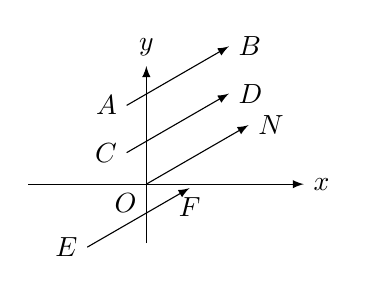
\begin{tikzpicture}
\pgfmathsetmacro{\k}{1.5}
\pgfmathsetmacro{\a}{30}
\draw[-latex](-1.5,0)--(2,0)node[right]{$x$};
\draw[-latex](0,-0.75)--(0,1.5)node[above]{$y$};
\draw[-latex](-0.25,1)node[left]{$A$}--++(\a:\k)node[right]{$B$};
\draw[-latex](-0.25,0.4)node[left]{$C$}--++(\a:\k)node[right]{$D$};
\draw[-latex](0,0)node[below left]{$O$}--++(\a:\k)node[right]{$N$};
\draw[-latex](-0.75,-0.8)node[left]{$E$}--++(\a:\k)node[below]{$F$};
\end{tikzpicture}
\caption{یکساں لمبائی اور یکساں رخ کے سمتیات ایک ہی سمتیہ کو ظاہر کرتے ہیں۔}
\label{شکل_مثال_سمتیہ_یکساں_چار}
\end{minipage}\hfill
\begin{minipage}{0.45\textwidth}
\centering
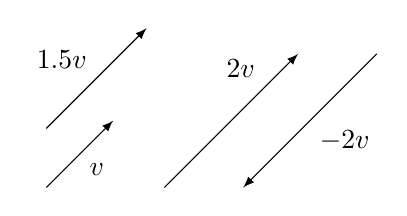
\begin{tikzpicture}
\pgfmathsetmacro{\k}{1.2}
\pgfmathsetmacro{\a}{45}
\draw[-latex](0,0)--++(\a:\k)node[pos=0.5,below right]{$\kvec{v}$};
\draw[-latex](0,0.75)--++(\a:1.5*\k)node[pos=0.5,above left]{$1.5\kvec{v}$};
\draw[-latex](1.5,0)--++(\a:2*\k)node[pos=0.75,above left]{$2\kvec{v}$};
\draw[latex-](2.5,0)--++(\a:2*\k)node[pos=0.5,below right]{$-2\kvec{v}$};
\end{tikzpicture}
\caption{سمتیہ کے غیر سمتی مضرب۔}
\label{شکل_سمتیہ_غیر_سمتی_مضرب}
\end{minipage}
\end{figure}
\جزوحصہء{غیر سمتیہ اور غیر سمتی مضرب}
ہم کسی سمتیہ کو مثبت حقیقی عدد سے ضرب دینے کے لئے اس کی لمبائی کو اس عدد سے ضرب دیتے ہیں (شکل \حوالہ{شکل_سمتیہ_غیر_سمتی_مضرب})۔ سمتیہ کو \عددی{2} سے ضرب دینے کے لئے ہم اس کی لمبائی دگنی کرتے ہیں۔ ایک سمتیہ کو \عددی{1.5} سے ضرب دینے کے لئے ہم اس کی لمبائی \عددی{\SI{50}{\percent}} بڑھاتے ہیں، وغیرہ، وغیرہ۔ ایک سمتیہ کو منفی  عدد سے ضرب دینے کے لئے ہم اس کا رخ الٹ کر کے اس کی لمبائی کو عدد کی مطلق قیمت سے ضرب دیتے ہیں۔

اگر \عددی{c} غیر صفر حقیقی عدد اور \عددی{\kvec{v}} ایک سمتیہ ہو تب مثبت \عددی{c} کی صورت میں \عددی{\kvec{v}} اور \عددی{c\kvec{v}} کے رخ ایک جیسے ہوں گے جبکہ منفی \عددی{c} کی صورت میں ان کے رخ ایک دوسرے کے مخالف ہوں گے۔ یہاں حقیقی اعداد تبدیلی پیمانہ کے طور پر کام کرتے ہیں اور یہ  \اصطلاح{غیر سمتی}\فرہنگ{غیر سمتی}\حاشیہب{scalar}\فرہنگ{scalar} کہلاتے ہیں جبکہ \عددی{c\kvec{v}} کے مضرب کو \عددی{\kvec{v}} کا \اصطلاح{غیر سمتی مضرب}\فرہنگ{غیر سمتی!مضرب}\حاشیہب{scalar multiple}\فرہنگ{scalar multiple} کہتے ہیں۔

صفر سے ضرب کو شامل کرنے کی خاطر ہم  اس روایت کو اپناتے ہیں جس کے  مطابق کسی بھی سمتیہ کو صفر سے ضرب دینے سے \اصطلاح{صفر سمتیہ} \عددی{\kvec{0}} حاصل ہو گا، جو ایک نقطہ پر مشتمل ہو گا جس کی لمبائی صفر ہو گی۔ دیگر سمتیہ کے برعکس صفر سمتیہ \عددی{\kvec{0}} کا کوئی رخ نہیں ہوتا ہے۔  

\جزوحصہء{جیومیٹریائی مجموعہ: قاعدہ متوازی الاضلاع}
دو غیر صفر سمتیات \عددی{\kvec{v}_1} اور \عددی{\kvec{v}_2} کا جیومیٹریائی مجموعہ لینے کی خاطر \عددی{\kvec{v}_1} کا نمائندہ، مثلاً \عددی{A} سے \عددی{B} تک، ترسیم کر کے \عددی{\kvec{v}_1} کے اختتامی نقطہ (سر) \عددی{B} پر \عددی{\kvec{v}_2}  کے نمائندہ کا ابتدائی نقطہ (دم)  رکھ کر ترسیم کریں۔ شکل \حوالہ{شکل_سمتیات_کا_مجموعہ} میں
$\kvec{v}_2=\krightharpoonup{BC}$
ہے۔ مجموعہ \عددی{\kvec{v}_1+\kvec{v}_2} اب \عددی{\kvec{v}_1} کے دم  \عددی{A} سے \عددی{\kvec{v}_2} کے سر  \عددی{C} تک سمتیہ ہو گا۔ یوں اگر
\begin{align*}
\kvec{v}_1=\overset{\rightharpoonup}{\rule{0pt}{.9ex}\smash{AB}},\quad \kvec{v}_2=\krightharpoonup{BC}
\end{align*}
ہوں تب
\begin{align*}
\kvec{v}_1+\kvec{v}_2=\krightharpoonup{AB}+\krightharpoonup{BC}=\krightharpoonup{AC}
\end{align*}
ہو گا۔چونکہ اس عمل میں \عددی{\kvec{v}_1+\kvec{v}_2} متوازی الاضلاع کا وتر ہوتا ہے لہٰذا اس عمل کو بعض اوقات \اصطلاح{قاعدہ متوازی الاضلاع}\فرہنگ{قاعدہ!متوازی الاضلاع}\حاشیہب{parallelogram law}\فرہنگ{law!parallelogram} کہتے ہیں (شکل \حوالہ{شکل_سمتیہ_قاعدہ_متوازی_الاضلاع})۔
\begin{figure}
\centering
\begin{minipage}{0.45\textwidth}
\centering
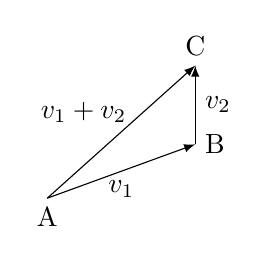
\begin{tikzpicture}
\draw[-latex](0,0)node[below]{A}--(20:2)node[pos=0.5,below]{$\kvec{v}_1$}node[right]{B};
\draw[-latex](20:2)--++(90:1)node[above]{C}node[pos=0.5,right]{$\kvec{v}_2$};
\draw[latex-](20:2)++(90:1)--(0,0)node[pos=0.4,left,yshift=0.5ex]{$\kvec{v}_1+\kvec{v}_2$};
\end{tikzpicture}
\caption{سمتیات \عددی{\kvec{v}_1} اور \عددی{\kvec{v}_2} کا مجموعہ۔}
\label{شکل_سمتیات_کا_مجموعہ}
\end{minipage}\hfill
\begin{minipage}{0.45\textwidth}
\centering
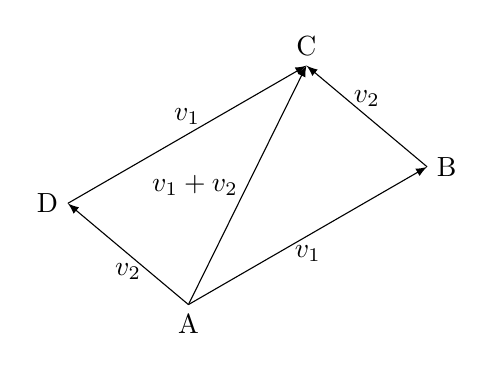
\begin{tikzpicture}
\pgfmathsetmacro{\da}{3.5}
\pgfmathsetmacro{\aa}{30}
\pgfmathsetmacro{\db}{2}
\pgfmathsetmacro{\ab}{140}
\draw[-latex](0,0)node[below]{A}--++(\aa:\da)node[right]{B}node[pos=0.5,below]{$\kvec{v}_1$}coordinate(kB);
\draw[-latex](kB)--++(\ab:\db)node[above]{C}node[pos=0.5,above]{$\kvec{v}_2$}coordinate(kC);
\draw[-latex](0,0)--++(\ab:\db)node[left]{D}node[pos=0.5,below]{$\kvec{v}_2$}coordinate(kD);
\draw[-latex](kD)--++(\aa:\da)node[pos=0.5,above]{$\kvec{v}_1$};
\draw[-latex](0,0)--(kC)node[pos=0.5,left]{$\kvec{v}_1+\kvec{v}_2$};
\end{tikzpicture}
\caption{قاعدہ متوازی الاضلاع۔ مخالف اضلاع یکساں لمبائی ہونے کی بنا \عددی{ABCD} متوازی الاضلاع ہو گا۔}
\label{شکل_سمتیہ_قاعدہ_متوازی_الاضلاع}
\end{minipage}
\end{figure}
\جزوحصہء{اجزاء}
دو سمتیات اس صورت متوازی ہوں گے جب یہ ایک دوسرے کے غیر صفر، غیر سمتی مضرب ہوں، یعنی جب ان کو ظاہر کرنے والے خطوط متوازی ہوں۔

جب بھی ایک سمتیہ \عددی{\kvec{v}} کو دو غیر متوازی سمتیات کا مجموعہ
\begin{align*}
\kvec{v}=\kvec{v}_1+\kvec{v}_2
\end{align*}
لکھنا ممکن ہو، سمتیات \عددی{\kvec{v}_1} اور \عددی{\kvec{v}_2} سمتیہ \عددی{\kvec{v}} کے اجزاء کہلائیں گے  اور ہم کہتے ہیں کہ  سمتیہ  \عددی{\kvec{v}} کو اس کے  اجزاء \عددی{\kvec{v}_1} اور \عددی{\kvec{v}_2} میں تحلیل کیا گیا ہے۔

سمتیات کے  مقبول ترین الجبرا میں ہر سمتیہ کو کارتیسی محور کے متوازی اجزاء کی صورت میں بیان کیا جاتا ہے اور یہ اجزاء از خود موزوں \اصطلاح{اساسی}\فرہنگ{اساسی}\حاشیہب{basic}\فرہنگ{basic} سمتیہ، جن کی لمبائی \عددی{1} ہوتی ہے، کے مضرب ہوتے ہیں۔ مثبت \عددی{x} محور کے رخ اساسی سمتیہ نقطہ \عددی{(0,0)} سے نقطہ \عددی{(1,0)} تک تیر سے ظاہر کیا جاتا ہے  اور اس اساسی سمتیہ کی علامت  \عددی{\ai} ہے۔ مثبت \عددی{y} محور کے رخ اساسی سمتیہ نقطہ \عددی{(0,0)} سے نقطہ \عددی{(0,1)} تک تیر سے ظاہر کیا جاتا ہے اور اس اساسی سمتیہ کی علامت  \عددی{\aj} ہے۔ اب غیر سمتی \عددی{a} کے لئے  محور \عددی{x} کے متوازی  سمتیہ \عددی{a\ai}  کی لمبائی \عددی{\abs{a}} ہو گی جبکہ اس کا رخ \عددی{a>0} کے لئے  دایاں اور  \عددی{a<0} کے لئے بایاں ہو گا۔ اس طرح غیر سمتی \عددی{b} کے لئے  محور \عددی{y} کے متوازی  سمتیہ \عددی{b\aj}  کی لمبائی \عددی{\abs{b}} ہو گی جبکہ اس کا رخ \عددی{b>0} کے لئے  اوپر اور  \عددی{b<0} کے لئے نیچے ہو گا۔ شکل \حوالہ{شکل_سمتیہ_اساسی} میں سمتیہ 
$\kvec{v}=\krightharpoonup{AC}$
کو اجزاء \عددی{\ai} اور \عددی{\aj} میں تحلیل کیا گیا ہے:
\begin{align*}
\kvec{v}=a\ai+b\aj
\end{align*}

\begin{figure}
\centering
\begin{minipage}{0.45\textwidth}
\centering
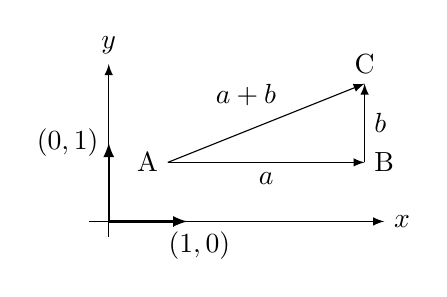
\begin{tikzpicture}
\pgfmathsetmacro{\a}{2.5}
\pgfmathsetmacro{\b}{1}
\draw[-latex](-0.25,0)--(3.5,0)node[right]{$x$};
\draw[-latex](0,-0.2)--(0,2)node[above]{$y$};
\draw[-latex] (0.75,0.75)coordinate(kA)node[left]{A}--++(\a,0)node[pos=0.5,below]{$a\ai$}node[right]{B}coordinate(kB);
\draw[-latex](kB)--++(0,\b)node[above]{C}node[pos=0.5,right]{$b\aj$};
\draw[-latex](kA)--++(\a,\b)node[pos=0.6,above left]{$a\ai+b\aj$};
\draw[-latex,thick](0,0)--(1,0)node[below,xshift={1ex}]{$(1,0)$}node[pos=0.5,below]{$\ai$};
\draw[-latex,thick](0,0)--(0,1)node[left]{$(0,1)$}node[pos=0.5,left]{$\aj$};
\end{tikzpicture}
\caption{اساس سمتیات \عددی{\ai} اور \عددی{\aj} کو استعمال کر کے کسی بھی سمتیہ \عددی{\krightharpoonup{AC}} کو لکھا جا سکتا ہے۔}
\label{شکل_سمتیہ_اساسی}
\end{minipage}\hfill
\begin{minipage}{0.45\textwidth}
\centering
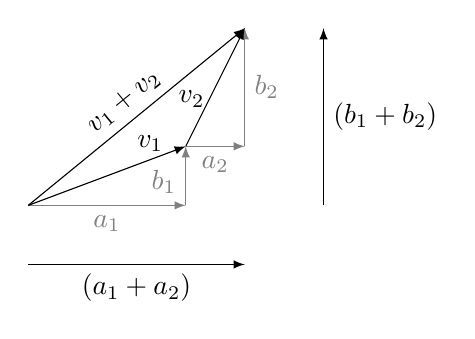
\begin{tikzpicture}
\pgfmathsetmacro{\a}{2}
\pgfmathsetmacro{\b}{0.75}
\pgfmathsetmacro{\c}{0.75}
\pgfmathsetmacro{\d}{1.5}
\draw[-latex,gray] (0,0)coordinate(kA)--++(\a,0)node[pos=0.5,below]{$a_1\ai$}coordinate(kB);
\draw[-latex,gray](kB)--++(0,\b)coordinate(kC)node[pos=0.4,left]{$b_1\aj$};
\draw[-latex](kA)--++(\a,\b)node[pos=0.85,shift={(-1ex,1ex)}]{$\kvec{v}_1$};
\draw[-latex,gray] (kC)coordinate(kAA)--++(\c,0)node[pos=0.5,below]{$a_2\ai$}coordinate(kBB);
\draw[-latex,gray](kBB)--++(0,\d)node[pos=0.5,right]{$b_2\aj$};
\draw[-latex](kAA)--++(\c,\d)node[pos=0.3,shift={(-1ex,1ex)}]{$\kvec{v}_2$}coordinate(kCC);
\draw[-latex](kA)--(kCC)node[pos=0.5,sloped,above]{$\kvec{v}_1+\kvec{v}_2$};
\draw[-latex](0,-0.75)--++(\a+\c,0)node[pos=0.5,below]{$(a_1+a_2)\ai$};
\draw[-latex](\a+\c+1,0)--++(0,\b+\d)node[pos=0.5,right]{$(b_1+b_2)\aj$};
\end{tikzpicture}
\caption{سمتیات کا مجموعہ ان کے مطابقتی اجزاء کے مجموعہ لے کر حاصل ہو گا۔}
\label{شکل_سمتیات_مجموعی_اجزاء}
\end{minipage}
\end{figure}

\ابتدا{تعریف}
اگر \عددی{\kvec{v}=a\ai+b\aj} ہو تب \عددی{\ai} اور \عددی{\aj} کے رخ، سمتیہ \عددی{\kvec{v}} کے اجزاء  سمتیات \عددی{a\ai} اور \عددی{b\aj} ہوں گے۔ اعداد \عددی{a} اور \عددی{b}، اساسی سمتیات \عددی{\ai} اور \عددی{\aj} کے رخ، سمتیہ \عددی{\kvec{v}} کے غیر سمتی اجزاء ہوں گے۔ 
\انتہا{تعریف}
%================

\ابتدا{تعریف}
سمتیات کی برابری یا یکسانیت (الجبرائی تعریف)۔
\begin{align}
a\ai+b\aj=a'\ai+b'\aj\quad \Leftrightarrow\quad a=a',\quad b=b'
\end{align}
\انتہا{تعریف}
%=======

دو سمتیات صرف اور صرف اس صورت ایک دوسرے کے برابر ہوں گے جب \عددی{\ai} اور \عددی{\aj} کے رخ، ان کے مطابقتی غیر سمتی اجزاء ایک دوسرے کے برابر ہوں۔

\جزوحصہء{الجبرائی مجموعہ}
سمتیات کے مطابقتی غیر سمتی اجزاء کا مجموعہ لے کر ان سمتیات  کا مجموعہ حاصل کیا جا سکتا ہے (شکل \حوالہ{شکل_سمتیات_مجموعی_اجزاء})۔

اگر \عددی{\kvec{v}_1=a_1\ai+b_1\aj} اور \عددی{\kvec{v}_2=a_2\ai+b_2\aj} ہوں تب درج ذیل ہو گا۔ 
\begin{align*}
\kvec{v}_1+\kvec{v}_2=(a_1+a_2)\ai+(b_1+b_2)\aj
\end{align*}

\ابتدا{مثال}
\begin{align*}
(2\ai-4\aj)+(5\ai+3\aj)=(2+5)\ai+(-4+3)\aj=7\ai-\aj
\end{align*}
\انتہا{مثال}

\begin{figure}
\centering
\begin{subfigure}{0.30\textwidth}
\centering
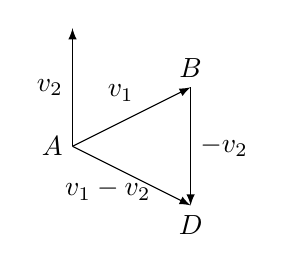
\begin{tikzpicture}
\pgfmathsetmacro{\a}{1.5}
\pgfmathsetmacro{\b}{0.75}
\pgfmathsetmacro{\aa}{0}
\pgfmathsetmacro{\bb}{1.5}
\draw[-latex](0,0)node[left]{$A$}--++(\a,\b)node[pos=0.6,above left]{$\kvec{v}_1$}node[above]{$B$}coordinate(kB);
\draw[-latex](0,0)--++(\aa,\bb)node[pos=0.5,left]{$\kvec{v}_2$};
\draw[-latex](kB)--++(\aa,-\bb)node[pos=0.5,right]{$-\kvec{v}_2$}coordinate(kD)node[below]{$D$};
\draw[-latex](0,0)--(kD)node[pos=0.4,below,xshift={-1ex}]{$\kvec{v}_1-\kvec{v}_2$};
\end{tikzpicture}
\caption{}
\end{subfigure}\hfill
\begin{subfigure}{0.30\textwidth}
\centering
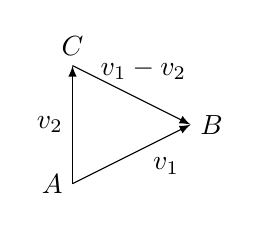
\begin{tikzpicture}
\pgfmathsetmacro{\a}{1.5}
\pgfmathsetmacro{\b}{0.75}
\pgfmathsetmacro{\aa}{0}
\pgfmathsetmacro{\bb}{1.5}
\draw[-latex](0,0)node[left]{$A$}--++(\a,\b)node[right]{$B$}node[pos=0.6,below right]{$\kvec{v}_1$}coordinate(kB);
\draw[-latex](0,0)--++(\aa,\bb)node[above]{$C$}node[pos=0.5,left]{$\kvec{v}_2$}coordinate(kC);
\draw[-latex](kC)--(kB)node[pos=0.6,above,yshift={1ex}]{$\kvec{v}_1-\kvec{v}_2$};
\end{tikzpicture}
\caption{}
\end{subfigure}\hfill
\begin{subfigure}{0.30\textwidth}
\centering
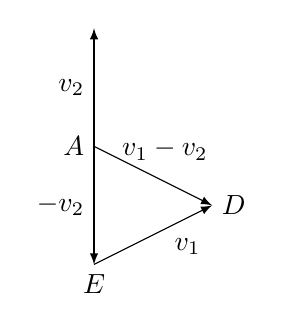
\begin{tikzpicture}
\pgfmathsetmacro{\a}{1.5}
\pgfmathsetmacro{\b}{0.75}
\pgfmathsetmacro{\aa}{0}
\pgfmathsetmacro{\bb}{1.5}
\draw[-latex](0,0)node[below]{$E$}--++(\a,\b)node[right]{$D$}node[pos=0.6,below right]{$\kvec{v}_1$}coordinate(kD);
\draw[latex-](0,0)--++(\aa,\bb)node[left]{$A$}node[pos=0.5,left]{$-\kvec{v}_2$}coordinate(kA);
\draw[-latex](kA)--(kD)node[pos=0.6,above,yshift={1ex}]{$\kvec{v}_1-\kvec{v}_2$};
\draw[-latex](kA)--++(\aa,\bb)node[pos=0.5,left]{$\kvec{v}_2$};
\end{tikzpicture}
\caption{}
\end{subfigure}
\caption{سمتیہ \عددی{\kvec{v}_1-\kvec{v}_2} کو ترسیم کرنے کے کئی طریقوں میں سے تین طریقے۔}
\label{شکل_سمتیہ_تفریق_طریقے}
\end{figure}

\جزوحصہء{تفریق}
ایک سمتیہ \عددی{\kvec{v}} کا منفی سمتیہ \عددی{-\kvec{v}=(-1)\kvec{v}} ہو گا۔ اس کی لمبائی \عددی{\kvec{v}} کی لمبائی ہو گی البتہ اس کا رخ \عددی{\kvec{v}} کا مخالف ہو گا۔سمتیہ \عددی{\kvec{v}_2} کو سمتیہ \عددی{\kvec{v}_1} سے منفی کرنے کی خاطر ہم  \عددی{-\kvec{v}_2} اور \عددی{\kvec{v}_1} کا مجموعہ لیں گے۔ جیومیٹریائی طور پر ہم \عددی{\kvec{v}_1} کے سر سے \عددی{-\kvec{v}_2} کھینچ کر \عددی{\kvec{v}_1} کے دم سے \عددی{-\kvec{v}_2} کے سر تک سمتیہ ترسیم کریں گے۔ یہ عمل شکل \حوالہ{شکل_سمتیہ_تفریق_طریقے}-ا میں دکھایا گیا ہے جہاں 
\begin{align*}
\krightharpoonup{AD}=\krightharpoonup{AB}+\krightharpoonup{BD}=\kvec{v}_1+(-\kvec{v}_2)=\kvec{v}_1-\kvec{v}_2
\end{align*}

اس کے علاوہ  \عددی{\kvec{v}_1} اور \عددی{\kvec{v}_2} کے دم مشترکہ  نقطہ پر رکھ  کر \عددی{\kvec{v}_1} اور \عددی{\kvec{v}_2} ترسیم کر کے \عددی{\kvec{v}_2} کے سر سے \عددی{\kvec{v}_1} کے سر تک سمتیہ \عددی{\kvec{v}_1-\kvec{v}_2} ہو گا۔ یہ عمل  شکل \حوالہ{شکل_سمتیہ_تفریق_طریقے}-ب میں پیش  کیا گیا ہے جہاں درج ذیل ہے۔
 \begin{align*}
\krightharpoonup{CB}=\krightharpoonup{CA}+\krightharpoonup{AB}=-\kvec{v}_2+\kvec{v}_1=\kvec{v}_1-\kvec{v}_2
\end{align*}
مزید، \عددی{-\kvec{v}_2} کے سر سے \عددی{\kvec{v}_1} ترسیم کر کے \عددی{\kvec{v}_1-\kvec{v}_2} حاصل کیا جا سکتا ہے (شکل \حوالہ{شکل_سمتیہ_تفریق_طریقے}-ج)۔

درج ذیل قاعدہ سمتیات کی تفریق کو اجزاء کی صورت میں پیش کرتا ہے۔
\begin{align}
\kvec{v}_1-\kvec{v}_2=(a_1-a_2)\ai+(b_1-b_2)\aj
\end{align}
اس قاعدہ کے تحت دو سمتیات تفریق کرنے کی خاطر ان کے مطابقتی اجزاء تفریق کیے جائیں گے۔

\ابتدا{مثال}
\begin{align*}
(6\ai+2\aj)-(3\ai-5\aj)=(6-3)\ai+(2-(-5))\aj=3\ai+7\aj
\end{align*}
\انتہا{مثال}
%============================

ہم نقطہ \عددی{N_1(x_1,y_1)} سے نقطہ \عددی{N_2(x_2,y_2)} تک سمتیہ کے اجزاء حاصل کرنے کے لئے \عددی{\krightharpoonup{ON_1}=x_1\ai+y_1\aj} کے اجزاء کو \عددی{\krightharpoonup{ON_2}=x_2\ai+y_2\aj} کے اجزاء سے منفی کرتے ہیں۔

\عددی{N_1(x_1,y_1)} سے \عددی{N_2(x_2,y_2)} تک سمتیہ درج ذیل ہو گا۔
\begin{align}
\krightharpoonup{N_1N_2}=(x_2-x_1)\ai+(y_2-y_1)\aj
\end{align}

\begin{figure}
\centering
\begin{minipage}{0.55\textwidth}
\centering
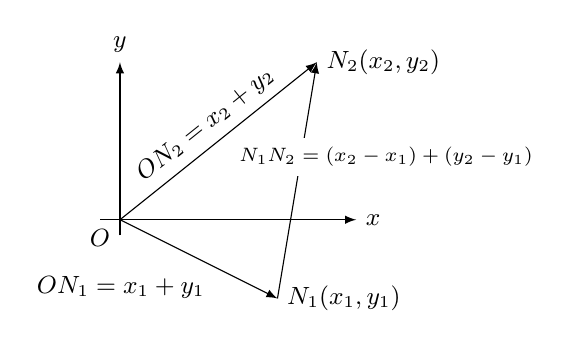
\begin{tikzpicture}[font=\small]
\pgfmathsetmacro{\a}{2}
\pgfmathsetmacro{\b}{-1}
\pgfmathsetmacro{\aa}{2.5}
\pgfmathsetmacro{\bb}{2}
\draw[-latex](-0.25,0)--(3,0)node[right]{$x$};
\draw[-latex](0,-0.2)--(0,2)node[above]{$y$};
\draw[-latex](0,0)node[below left]{$O$}--++(\a,\b)node[pos=0.6,below left]{$\krightharpoonup{ON_1}=x_1\ai+y_1\aj$}node[right]{$N_1(x_1,y_1)$}coordinate(kA);
\draw[-latex](0,0)--++(\aa,\bb)node[pos=0.5,sloped, above]{$\krightharpoonup{ON_2}=x_2\ai+y_2\aj$}node[right]{$N_2(x_2,y_2)$}coordinate(kB);
\draw[-latex](kA)--(kB)node[pos=0.6,fill=white,right,xshift=-6ex,font=\scriptsize]{$\krightharpoonup{N_1N_2}=(x_2-x_1)\ai+(y_2-y_1)\aj$};
\end{tikzpicture}
\caption{}
\end{minipage}\hfill
\begin{minipage}{0.35\textwidth}
\centering
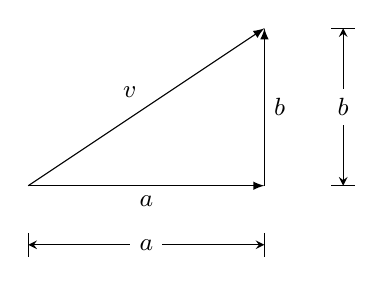
\begin{tikzpicture}[font=\small]
\pgfmathsetmacro{\a}{3}
\pgfmathsetmacro{\b}{2}
\draw[-latex](0,0)--++(\a,0)node[pos=0.5,below]{$a\ai$}coordinate(kA);
\draw[-latex](kA)--++(0,\b)node[pos=0.5,right]{$b\aj$}coordinate(kB);
\draw[-latex](0,0)--(kB)node[pos=0.5,above left]{$\kvec{v}$};
\draw[stealth-stealth](0,-0.75)--++(\a,0)node[pos=0.5,fill=white]{$\abs{a}$};
\draw[stealth-stealth](\a+1,0)--++(0,\b)node[pos=0.5,fill=white]{$\abs{b}$};
\draw(0,-0.6)--++(0,-0.3);
\draw(\a,-0.6)--++(0,-0.3);
\draw(\a+0.85,0)--++(0.3,0);
\draw(\a+0.85,\b)--++(0.3,0);
\end{tikzpicture}
\caption{سمتیہ کی لمبائی مسئلہ فیثاغورث سے حاصل کی جا سکتی ہے۔}
\label{شکل_سمتیہ_کی_لمبائی}
\end{minipage}
\end{figure}
\ابتدا{مثال}
نقطہ \عددی{N_1(3,4)} سے نقطہ \عددی{N_2(5,1)} تک سمتیہ درج ذیل ہے۔
\begin{align*}
\krightharpoonup{N_1N_2}=(5-3)\ai+(1-4)\aj=2\ai-3\aj
\end{align*}
\انتہا{مثال}
%===============

\جزوحصہء{مقدار}
سمتیہ \عددی{\kvec{v}=a\ai+b\aj} کی \اصطلاح{لمبائی}\فرہنگ{سمتیہ!لمبائی}\حاشیہب{length}\فرہنگ{vector!length} یا \اصطلاح{مقدار}\فرہنگ{سمتیہ!مقدار}\حاشیہب{magnitude}\فرہنگ{vector!magnitude} \عددی{\abs{\kvec{v}}=\sqrt{a^2+b^2}} ہے۔  سمتیہ \عددی{\kvec{v}} اور اس کے دو سمتیہ اجزاء کے قائمہ مثلث پر مسئلہ فیثاغورث لاگو کرنے سے یہ کلیہ اخذ ہوتا ہے (شکل \حوالہ{شکل_سمتیہ_کی_لمبائی})۔ سمتیہ کی لمبائی \عددی{\abs{\kvec{v}}} میں دو انتصابی لکیریں وہی ہیں جو مطلق قیمت کو ظاہر کرنے کے لئے استعمال کی جاتی ہیں۔ 

\begin{align}
\abs{\kvec{v}}&=\sqrt{a^2+b^2}&&\kvec{v}=a\ai+b\aj
\end{align}

\ابتدا{مثال}\شناخت{مثال_سمتیہ_ہاتھ_ریڑھی}
آپ زمین کے ساتھ \عددی{30^{\circ}} زاویہ پر \عددی{\SI{20}{\newton}} کی قوت \عددی{\kvec{F}} سے ہاتھ ریڑھی کو دکھا لگاتے ہیں (شکل \حوالہ{شکل_مثال_سمتیہ_ہاتھ_ریڑھی}-ا)۔ قوت کا افقی جزو ریڑھی کو حرکت دیتا ہے جبکہ اس کا انتصابی جزو ریڑھی کا وزن بڑھاتا ہے۔ اس قوت کا افقی اور انتصابی جزو معلوم کریں۔

حل:\quad
ہم قوت \عددی{\kvec{F}=a\ai+b\aj} اور اس کے اجزاء کے لئے مثلث  بناتے ہیں (شکل \حوالہ{شکل_مثال_سمتیہ_ہاتھ_ریڑھی}-ب اور شکل \حوالہ{شکل_مثال_سمتیہ_ہاتھ_ریڑھی}-ج)۔ اس مثلث سے \عددی{a=10\sqrt{3}} اور \عددی{b=10} حاصل ہوتے ہیں۔ قوت کا افقی جزو \عددی{10\sqrt{3}\ai} اور انتصابی جزو \عددی{-10\aj} ہے۔یوں \عددی{\kvec{F}=10\sqrt{3}\ai-10\aj} ہو گا۔  انتصابی جزو کا رخ نیچے ہے لہٰذا یہ منفی ہے۔ 
\انتہا{مثال}
%==================
\begin{figure}
\centering
\begin{subfigure}{0.30\textwidth}
\centering
\begin{tikzpicture}
\pgfmathsetmacro{\kx}{1.5}
\pgfmathsetmacro{\ky}{0.5}
\pgfmathsetmacro{\r}{0.1}
\pgfmathsetmacro{\len}{2}
\pgfmathsetmacro{\ang}{150}
\draw(0,0)--++(\kx,0)--++(0,-\ky)--++(-\kx,0)--++(0,\ky);
\draw(1/2*\kx,-1/2*\ky)node[]{\RL{ہاتھ ریڑھی}};
\draw([shift={(180:\r)}]1/4*\kx,-\ky) arc (180:360:\r);
\draw([shift={(180:\r)}]3/4*\kx,-\ky) arc (180:360:\r);
\draw[latex-](0,0)--++(\ang:\len)node[pos=0.5,above right]{$\abs{\kvec{F}}=20$};
\draw[dashed](0,0)--(-2,0);
\draw[]([shift={(\ang:0.5)}]0,0) arc (\ang:180:0.5)node[pos=0.3,left]{$30^{\circ}$};
\end{tikzpicture}
\caption{}
\end{subfigure}\hfill
\begin{subfigure}{0.30\textwidth}
\centering
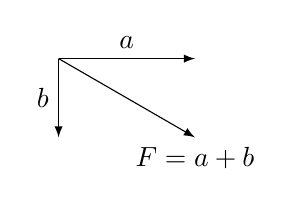
\begin{tikzpicture}
\pgfmathsetmacro{\len}{2}
\pgfmathsetmacro{\ang}{150}
\pgfmathsetmacro{\a}{\len*cos(180-\ang)}
\pgfmathsetmacro{\b}{\len*sin(\ang)}
\draw[-latex](0,0)--(\a,0)node[pos=0.5,above]{$a\ai$};
\draw[-latex](0,0)--(0,-\b)node[pos=0.5,left]{$b\aj$};
\draw[-latex](0,0)--++(\ang-180:\len)node[below]{$\kvec{F}=a\ai+b\aj$};
\end{tikzpicture}
\caption{}
\end{subfigure}\hfill
\begin{subfigure}{0.30\textwidth}
\centering
\begin{tikzpicture}[font=\small]
\pgfmathsetmacro{\len}{2}
\pgfmathsetmacro{\ang}{150}
\pgfmathsetmacro{\a}{\len*cos(180-\ang)}
\pgfmathsetmacro{\b}{\len*sin(\ang)}
\draw[](0,-\b)--++(\a,0)node[pos=0.5,below]{$\abs{a\ai}=a$};
\draw[](0,0)--(0,-\b)node[below left]{$B$}node[pos=0.5,left]{$\abs{b\aj}=b$};
\draw[](0,0)node[above]{$A$}--++(\ang-180:\len)node[below right]{$C$}node[pos=0.3,above right]{$\abs{\kvec{F}}=20$};
\draw([shift={(270:0.3)}]0,0) arc (270:330:0.3)node[pos=0.6,below]{$\tfrac{\pi}{3}$};
\draw([shift={(\ang:0.6)}]\a,-\b) arc (\ang:180:0.6)node[pos=0.35,left]{$\tfrac{\pi}{6}$};
\end{tikzpicture}
\caption{}
\end{subfigure}
\caption{ہاتھ ریڑھی (مثال \حوالہ{مثال_سمتیہ_ہاتھ_ریڑھی})}
\label{شکل_مثال_سمتیہ_ہاتھ_ریڑھی}
\end{figure}
\جزوحصہء{غیر سمتی ضرب}
غیر سمتی ضرب جزو در جزو حاصل کیا جا سکتا ہے۔ اگر \عددی{c} ایک غیر سمتی اور \عددی{\kvec{v}=a\ai+b\aj} ایک سمتیہ ہو تب درج ذیل ہو گا۔
\begin{align}
c\kvec{v}=c(a\ai+b\aj)=(ca)\ai+(cb)\aj
\end{align}
سمتیہ \عددی{c\kvec{v}} کی لمبائی سمتیہ \عددی{\kvec{v}} کی لمبائی ضرب \عددی{\abs{c}} ہو گا:
\begin{align*}
\abs{c\kvec{v}}&=\abs{(ca)\ai+(cb)\aj}\\
&=\sqrt{(ca)^2+(cb)^2}\\
&=\sqrt{c^2(a^2+b^2)}\\
&=\sqrt{c^2}\sqrt{a^2+b^2}\\
&=\abs{c}\abs{\kvec{v}}
\end{align*}

یوں اگر \عددی{c} غیر سمتی ہو اور \عددی{\kvec{v}} ایک سمتیہ ہو تب \عددی{\abs{c\kvec{v}}=\abs{c}\abs{\kvec{v}}} ہو گا۔

\ابتدا{مثال}
اگر \عددی{c=-2} اور \عددی{\kvec{v}=-3\ai+4\aj} ہوں تب درج ذیل ہو گا۔
\begin{align*}
\abs{\kvec{v}}&=\abs{-3\ai+4\aj}=\sqrt{(-3)^2+(4)^2}=\sqrt{9+16}=\sqrt{25}=5\\
\abs{-2\kvec{v}}&=\abs{(-2)(-3\ai+4\aj)}=\abs{6\ai-8\aj}=\sqrt{(6)^2+(-8)^2}\\
&=\sqrt{36+64}=\sqrt{100}=10=\abs{-2}\abs{5}=\abs{c}\abs{\kvec{v}}
\end{align*}
\انتہا{مثال}
%======================

\جزوحصہء{صفر سمتیہ}
صفر سمتیہ سے مراد درج ذیل سمتیہ ہے۔
\begin{align*}
\kvec{0}=0\ai+0\aj
\end{align*}
دھیان رہے کہ صفر سمتیہ \عددی{\kvec{0}} کو ظاہر کرنے کے لئے \عددی{0} کو موٹی لکھائی میں لکھا جاتا ہے۔صفر سمتیہ وہ واحد سمتیہ ہے جس کی لمبائی صفر ہے۔ یہ حقیقت درج ذیل سے واضح ہے۔
\begin{align*}
\abs{a\ai+b\aj}=\sqrt{a^2+b^2}=0\quad \Leftrightarrow\quad a=b=0
\end{align*}

\begin{figure}
\centering
\begin{tikzpicture}[font=\small]
\pgfmathsetmacro{\r}{1.5}
\pgfmathsetmacro{\ang}{40}
\pgfmathsetmacro{\a}{\r*cos(\ang)}
\pgfmathsetmacro{\b}{\r*sin(\ang)}
\draw[-latex](-1.25*\r,0)--(1.75*\r,0)node[right]{$x$};
\draw[-latex](0,-1.1*\r)--(0,1.5*\r)node[above]{$y$};
\draw(0,0) circle (\r);
\draw[-latex,thick](0,0)--(\r,0)node[below right]{$(1,0)$};
\draw[-latex,thick](0,0)--(0,\r)node[above left]{$(0,1)$}node[pos=0.5,left]{$\aj$};
\draw[-latex,thick](0,0)--++(\ang:\r)node[pos=0.65,above]{$\kvec{u}$};
\draw[-latex,thick](0,0)--++(\a,0)node[pos=0.5,below]{$(\cos\theta)\ai$};
\draw[-latex,thick](\a,0)--++(0,\b)node[pos=0.5,right,fill=white]{$(\sin\theta)\aj$};
\draw[-stealth]([shift={(0:0.5)}]0,0) arc (0:\ang:0.5)node[pos=0.6,right]{$\theta$};
\draw(135:\r)node[pin=135:{\RL{اکائی دائرہ}}]{};
\end{tikzpicture}
\caption{مستوی میں ہر اکائی سمتیہ کو \عددی{\kvec{u}=(\cos\theta)\ai+(\sin\theta)\aj} روپ میں لکھا جا سکتا ہے۔}
\label{شکل_سمتیہ_اکائی_دائرہ}
\end{figure}
\جزوحصہء{اکائی سمتیات}
کوئی بھی سمتیہ جس کی لمبائی \عددی{1} ہو \اصطلاح{اکائی سمتیہ}\فرہنگ{سمتیہ!اکائی}\حاشیہب{unit vector}\فرہنگ{vector!unit} کہلائے گا۔ سمتیات \عددی{\ai} اور \عددی{\aj} اکائی سمتیات ہیں۔
\begin{align*}
\abs{\ai}=\abs{1\ai+0\aj}=\sqrt{1^2+0^2}=1,\quad \abs{\aj}=\abs{0\ai+1\aj}=\sqrt{0^2+1^2}=1
\end{align*}

سمتیہ \عددی{\kvec{u}} جو اکائی سمتیہ \عددی{\ai} کو  \عددی{\theta} زاویہ مثبت رخ گھما کر حاصل ہو گا،  کے سمتی اجزاء درج ذیل ہوں گے (شکل \حوالہ{شکل_سمتیہ_اکائی_دائرہ})۔
\begin{align}
\kvec{u}=(\cos\theta)\ai+(\sin\theta)\aj
\end{align}
چونکہ اکائی سمتیہ کو گھمانے سے اس کی لمبائی تبدیل نہیں ہوتی لہٰذا \عددی{\kvec{u}} بھی اکائی سمتیہ ہو گا یعنی:
\begin{align*}
\abs{\kvec{u}}=\sqrt{(\cos\theta)^2+(\sin\theta)^2}=\sqrt{1^2}=1
\end{align*}
زاویہ \عددی{\theta} کو \عددی{0} تا \عددی{2\pi} کرنے سے \عددی{\kvec{u}} کا سر \عددی{N} مبدا کے گرد، گھڑی کے الٹ رخ،  دائرہ \عددی{x^2+y^2=1} پر چلتا ہے جو مستوی میں ہر ممکنہ رخ  کا اکائی سمتیہ دے گا۔

\جزوحصہء{لمبائی اور رخ}
اگر \عددی{\kvec{v}\ne \kvec{0}} ہو تب
\begin{align*}
\abs{\frac{\kvec{v}}{\abs{\kvec{v}}}}=\abs{\frac{1}{\abs{\kvec{v}}}\kvec{v}}=\frac{1}{\abs{\kvec{v}}}\abs{\kvec{v}}=1
\end{align*}
ہو گا لہٰذا \عددی{\tfrac{\kvec{v}}{\abs{\kvec{v}}}} اکائی سمتیہ ہو گا جس کا رخ \عددی{\kvec{v}} کا رخ ہو گا۔یوں ہم \عددی{\kvec{v}} کو اس کی دو اہم خواص، لمبائی اور رخ، کی صورت میں درج ذیل لکھ سکتے ہیں۔
\begin{align*}
\kvec{v}=\abs{\kvec{v}}\big(\tfrac{\kvec{v}}{\abs{\kvec{v}}}\big)
\end{align*}

یوں اگر \عددی{\kvec{u}\ne \kvec{0}} ہو تب
\begin{enumerate}[a.]
\item
\عددی{\tfrac{\kvec{v}}{\abs{\kvec{v}}}} اکائی سمتیہ ہو گا جس کا رخ \عددی{\kvec{v}} کا رخ ہو گا۔ یوں ہم \عددی{\tfrac{\kvec{v}}{\abs{\kvec{v}}}} کو \عددی{\kvec{v}} کو رخ کہتے ہیں۔
\item
مساوات \عددی{\kvec{v}=\abs{\kvec{v}}(\tfrac{\kvec{v}}{\abs{\kvec{v}}})} سمتیہ \عددی{\kvec{v}} کو اس کی لمبائی اور رخ کی صورت میں  بیان کرتی ہے۔
\end{enumerate}

\ابتدا{مثال}
سمتیہ \عددی{\kvec{v}=3\ai-4\aj} کو اس کی لمبائی اور رخ کا حاصل ضرب لکھیں۔
 
حل:\quad
\begin{align*}
\abs{\kvec{v}}&=\sqrt{(3)^2+(-4)^2}=\sqrt{9+16}=5&&\text{\RL{\عددی{\kvec{v}} کی لمبائی}}\\
\frac{\kvec{v}}{\abs{\kvec{v}}}&=\frac{3\ai-4\aj}{5}=\frac{3}{5}\ai-\frac{4}{5}\aj&&\text{\RL{\عددی{\kvec{v}} کا رخ}}\\
\kvec{v}&=3\ai-4\aj=\underbrace{5}_{\text{لمبائی}}\big(\underbrace{\frac{3}{5}\ai-\frac{4}{5}\aj}_{\text{رخ}}\big)
\end{align*}
\انتہا{مثال}
%====================

\جزوحصہء{ڈھلوان، مماس اور عمود}
ایک سمتیہ اس صورت ایک خط کے متوازی ہو گا جب سمتیہ کو ظاہر کرنے والا قطع اور یہ خط متوازی ہوں۔ ایک غیر انتصابی سمتیہ کی ڈھلوان ان خطوط کی ڈھلوان ہو گی جو اس سمتیہ کے متوازی ہوں۔ یوں \عددی{a\ne 0} کی صورت میں سمتیہ \عددی{\kvec{v}=a\ai+b\aj} کا ڈھلوان \عددی{\tfrac{b}{a}} ہو گا (شکل \حوالہ{شکل_سمتیہ_ڈھلوان_تعریف})۔

کسی نقطہ پر ایک منحنی کو ایک سمتیہ تب \اصطلاح{مماسی}\فرہنگ{مماس}\حاشیہب{tangent}\فرہنگ{tangent} یا \اصطلاح{عمودی}\فرہنگ{عمودی}\حاشیہب{normal}\فرہنگ{normal} ہو گا جب اس نقطہ پر منحنی کا مماس  اور یہ سمتیہ متوازی یا عمودی ہوں۔ اگلی مثال میں ایسی سمتیہ کو تلاش کرنا دکھایا گیا ہے۔
\begin{figure}
\centering
\begin{minipage}{0.45\textwidth}
\centering
\begin{tikzpicture}
\pgfmathsetmacro{\a}{3}
\pgfmathsetmacro{\b}{2}
\pgfmathsetmacro{\ang}{atan(\b/\a)}
\draw[-latex](0,0)--++(\a,0)node[pos=0.5,below]{$a\ai$};
\draw[-latex](\a,0)--++(0,\b)node[pos=0.5,right]{$b\aj$};
\draw[-latex](0,0)--(\a,\b)node[pos=0.5,left,xshift={-0.5ex}]{$a\ai+b\aj$};
\draw(\ang:2.5)node[pin=135:{ڈھلوان\,\عددی{\tfrac{b}{a}}}]{};
\draw[-stealth]([shift={(0:0.6)}]0,0) arc (0:\ang:0.6)node[pos=0.6,right]{$\theta$};
\end{tikzpicture}
\caption{اگر \عددی{a\ne 0} ہو تب سمتیہ \عددی{\kvec{v}=a\ai+b\aj} کی ڈھلوان \عددی{\tfrac{b}{a}} ہو گی۔}
\label{شکل_سمتیہ_ڈھلوان_تعریف}
\end{minipage}\hfill
\begin{minipage}{0.45\textwidth}
\centering
\begin{tikzpicture}[declare function={f(\x)=1/2*\x^3+1/2;}]
\begin{axis}[clip=false,small,axis equal,axis lines=middle,ymin=0,xlabel={$x$},ylabel={$y$},xlabel style={at={(current axis.right of origin)},anchor=west},ylabel style={at={(current axis.above origin)},anchor=south},xtick={1},ytick={1}]
\addplot[domain=0:1.5] {f(x)}node[above]{$y=\tfrac{x^3}{2}+\tfrac{1}{2}$};
\draw[-stealth](axis cs:1,1)--(axis cs:{1+2/sqrt(13)},{1+3/sqrt(13)})coordinate(ka)node[pos=0.5,right]{$\kvec{u}=\tfrac{2}{\sqrt{13}}\ai+\tfrac{3}{\sqrt{13}}\aj$};
\draw[-stealth](axis cs:1,1)--(axis cs:{1-2/sqrt(13)},{1-3/sqrt(13)})node[pos=0.5,right]{$-\kvec{u}$};
\draw[-stealth](axis cs:1,1)--(axis cs:{1-3/sqrt(13)},{1+2/sqrt(13)})node[above]{$\kvec{n}=-\tfrac{3}{\sqrt{13}}\ai+\tfrac{2}{\sqrt{13}}\aj$};
\draw[-stealth](axis cs:1,1)--(axis cs:{1+3/sqrt(13)},{1-2/sqrt(13)})coordinate(kb)node[pos=0.5,above]{$-\kvec{n}$};
\RightAngle{({1+2/sqrt(13)},{1+3/sqrt(13)})}{(1,1)}{({1+3/sqrt(13)},{1-2/sqrt(13)})}
\end{axis}
\end{tikzpicture}
\caption{ایک نقطہ پر ترسیم کا اکائی مماسی اور اکائی عمودی سمتیہ (مثال \حوالہ{مثال_سمتیہ_مماس_عمود})}
\label{شکل_مثال_سمتیہ_مماس_عمود}
\end{minipage}
\end{figure}
\ابتدا{مثال}\شناخت{مثال_سمتیہ_مماس_عمود}
نقطہ \عددی{(1,1)} پر منحنی \عددی{y=\tfrac{x^3}{2}+\tfrac{1}{2}} کو مماسی اور عمودی اکائی سمتیات تلاش کریں۔

حل:\quad
ہم نقطہ \عددی{(1,0)} پر منحنی کے مماس کے متوازی اور عمودی اکائی سمتیات معلوم کرتے ہیں (شکل \حوالہ{شکل_مثال_سمتیہ_مماس_عمود})۔

اس نقطہ پر منحنی کے مماس کی ڈھلوان درج ذیل ہو گی۔
\begin{align*}
y'=\left.\frac{3x^2}{2}\right\vert_{x=1}=\frac{3}{2}
\end{align*}
ہم اتنی ڈھلوان کی اکائی سمتیہ تلاش کرتے ہیں۔ سمتیہ \عددی{\kvec{v}=2\ai+3\aj} اور اس کے ہر غیر صفر مضرب کی ڈھلوان \عددی{\tfrac{3}{2}} ہے۔ سمتیہ  \عددی{\kvec{v}} کا ایسا مضرب معلوم کرنے کے لئے جس کی لمبائی \عددی{1} ہو ہم \عددی{\kvec{v}} کو 
\begin{align*}
\abs{\kvec{v}}=\sqrt{2^2+3^2}=\sqrt{13}
\end{align*}
سے تقسیم کرتے ہیں۔ یوں درج ذیل حاصل ہو گا۔
\begin{align*}
\kvec{u}=\frac{\kvec{v}}{\abs{\kvec{v}}}=\frac{2}{\sqrt{13}}\ai+\frac{3}{\sqrt{13}}\aj
\end{align*}
سمتیہ \عددی{\kvec{u}} کی لمبائی \عددی{1} ہے اور یہ \عددی{(1,1)} پر منحنی کا مماس ہے۔ درج ذیل سمتیہ
\begin{align*}
-\kvec{u}=-\frac{2}{\sqrt{13}}\ai-\frac{3}{\sqrt{13}}\aj
\end{align*}
جو مخالف  رخ ہے بھی \عددی{(1,1)} پر منحنی کا مماس ہو گا۔ کسی اضافی شرط کے بغیر ان میں سے کسی ایک اکائی مماسی سمتیہ کو دوسری اکائی مماسی سمتیہ پر فوقیت نہیں دی جا سکتی ہے۔

نقطہ \عددی{(1,1)} پر منحنی کا عمودی سمتیہ تلاش کرنے کی خاطر ہم ایسا اکائی سمتیہ معلوم کرتے ہیں جس کی ڈھلوان \عددی{\kvec{u}} کی ڈھلوان کے بالعکس متناسب کے منفی کے برابر ہو۔ ہم \عددی{\kvec{u}} کے غیر سمتی اجزاء کے مقامات آپس میں تبدیل کر کے اور ان میں سے کسی ایک کی علامت بدل کر ایسا سمتیہ معلوم کر سکتے ہیں۔ یوں درج ذیل حاصل ہو گا۔
\begin{align*}
\kvec{n}=-\frac{3}{\sqrt{13}}\ai+\frac{2}{\sqrt{13}}\aj,\quad \text{}\quad -\kvec{n}=\frac{3}{\sqrt{13}}\ai-\frac{2}{\sqrt{13}}\aj
\end{align*}  
یہاں بھی دونوں اکائی سمتیات دیے گئے نقطہ پر منحنی کو عمودی ہیں۔ ان دو عمودی اکائی سمتیات کا رخ ایک دوسرے کے الٹ ہے لیکن دونوں \عددی{(1,1)} پر منحنی کو عمودی ہیں۔
\انتہا{مثال}
%====================

\حصہء{سوالات}
\موٹا{جیومیٹری اور حساب}\\
\ابتدا{سوال}\شناخت{سوال_سمتیہ_الف}
مستوی میں پائے جانے والے سمتیات \عددی{\kvec{A}}، \عددی{\kvec{B}} اور \عددی{\kvec{C}} کو شکل \حوالہ{شکل_سوال_سمتیہ_الف} میں دکھایا گیا ہے۔ انہیں کاغذ پر اتار کر سر کے ساتھ دم جوڑ کر درج ذیل ترسیم کریں۔
\begin{multicols}{4}
\begin{enumerate}[a.]
\item
$\kvec{A}+\kvec{B}$
\item
$\kvec{A}+\kvec{B}+\kvec{C}$
\item
$\kvec{A}-2\kvec{B}$
\item
$\frac{1}{2}\kvec{A}-\kvec{C}$
\end{enumerate}
\end{multicols}
جوابات:\quad
شکل \حوالہ{شکل_سوال_سمتیہ_جوابات_چند_جمع_منفی}
\انتہا{سوال}
%=======================
\ابتدا{سوال}\شناخت{سوال_سمتیہ_ب}
مستوی میں پائے جانے والے سمتیات \عددی{\kvec{A}}، \عددی{\kvec{B}} اور \عددی{\kvec{C}} کو شکل \حوالہ{شکل_سوال_سمتیہ_ب} میں دکھایا گیا ہے۔ انہیں کاغذ پر اتار کر سر کے ساتھ دم جوڑ کر درج ذیل ترسیم کریں۔
\begin{multicols}{4}
\begin{enumerate}[a.]
\item
$\kvec{A}-\kvec{B}$
\item
$\kvec{A}+\kvec{B}+\kvec{C}$
\item
$2\kvec{A}-\frac{1}{2}\kvec{B}$
\item
$\kvec{A}-(\kvec{B}-\kvec{C})$
\end{enumerate}
\end{multicols}
\انتہا{سوال}
%=======================
\begin{figure}
\centering
\begin{minipage}{0.22\textwidth}
\centering
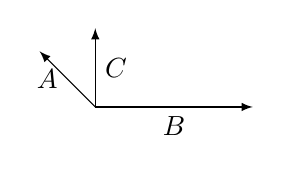
\begin{tikzpicture}
\pgfmathsetmacro{\a}{135}
\pgfmathsetmacro{\b}{1}
\pgfmathsetmacro{\aa}{0}
\pgfmathsetmacro{\bb}{2}
\pgfmathsetmacro{\aaa}{90}
\pgfmathsetmacro{\bbb}{1}
\draw[-latex](0,0)--(\a:\b)node[pos=0.5,left]{$A$};
\draw[-latex](0,0)--(\aa:\bb)node[pos=0.5,below]{$B$};
\draw[-latex](0,0)--(\aaa:\bbb)node[pos=0.5,right]{$C$};
\end{tikzpicture}
\caption{}
\label{شکل_سوال_سمتیہ_الف}
\end{minipage}\hfill
\begin{minipage}{0.22\textwidth}
\centering
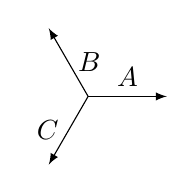
\begin{tikzpicture}
\pgfmathsetmacro{\a}{0}
\pgfmathsetmacro{\b}{1}
\pgfmathsetmacro{\aa}{120}
\pgfmathsetmacro{\bb}{1}
\pgfmathsetmacro{\aaa}{-120}
\pgfmathsetmacro{\bbb}{1}
\draw[-latex](0,0)--(\a:\b)node[pos=0.5,above]{$A$};
\draw[-latex](0,0)--(\aa:\bb)node[pos=0.5,right]{$B$};
\draw[-latex](0,0)--(\aaa:\bbb)node[pos=0.5,left]{$C$};
\end{tikzpicture}
\caption{}
\label{شکل_سوال_سمتیہ_ب}
\end{minipage}
\begin{minipage}{0.22\textwidth}
\centering
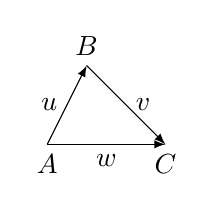
\begin{tikzpicture}
\draw[-latex](0,0)node[below]{$A$}--(1.5,0)node[pos=0.5,below]{$\kvec{w}$}node[below]{$C$};
\draw[-latex](0,0)--(0.5,1)node[pos=0.5,left]{$\kvec{u}$}node[above]{$B$};
\draw[-latex](0.5,1)--(1.5,0)node[pos=0.5,right]{$\kvec{v}$};
\end{tikzpicture}
\caption{}
\label{شکل_سوال_سمتیہ_پ}
\end{minipage}
\begin{minipage}{0.22\textwidth}
\centering
\begin{tikzpicture}
\draw[-latex](0,0)node[left]{$A$}--(2,0)node[pos=0.5,below]{$\kvec{w}$}node[right]{$C$};
\draw[-latex](0,0)--(0.5,1)node[pos=0.5,left]{$\kvec{u}$}node[above]{$B$};
\draw[-latex](0.5,1)--(2,0);
\draw[-latex](0,0)--(1.25,0.5)node[pos=0.5,above]{$\kvec{a}$}node[circ]{}node[right]{$N$};
\end{tikzpicture}
\caption{}
\label{شکل_سوال_سمتیہ_ت}
\end{minipage}
\end{figure}
%==================================================
\begin{figure}
\centering
\begin{subfigure}{0.45\textwidth}
\centering
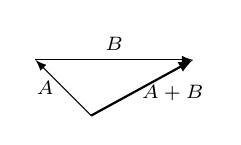
\begin{tikzpicture}[font=\scriptsize]
\pgfmathsetmacro{\a}{135}
\pgfmathsetmacro{\b}{1}
\pgfmathsetmacro{\aa}{0}
\pgfmathsetmacro{\bb}{2}
\pgfmathsetmacro{\aaa}{90}
\pgfmathsetmacro{\bbb}{1}
\draw[-latex](0,0)--(\a:\b)node[pos=0.5,left]{$A$};
\draw[-latex](\a:\b)--++(\aa:\bb)coordinate(khead)node[pos=0.5,above]{$B$};
\draw[thick,-latex](0,0)--++(khead)node[pos=0.4,right]{$A+B$};
\end{tikzpicture}
\caption{}
\end{subfigure}\hfill
\begin{subfigure}{0.45\textwidth}
\centering
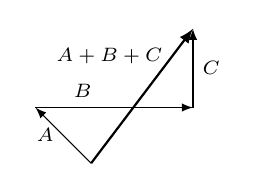
\begin{tikzpicture}[font=\scriptsize]
\pgfmathsetmacro{\a}{135}
\pgfmathsetmacro{\b}{1}
\pgfmathsetmacro{\aa}{0}
\pgfmathsetmacro{\bb}{2}
\pgfmathsetmacro{\aaa}{90}
\pgfmathsetmacro{\bbb}{1}
\draw[-latex](0,0)--(\a:\b)node[pos=0.5,left]{$A$};
\draw[-latex](\a:\b)--++(\aa:\bb)coordinate(ka)node[pos=0.3,above]{$B$};
\draw[-latex](ka)--++(\aaa:\bbb)coordinate(kb)node[pos=0.5,right]{$C$};
\draw[thick,-latex](0,0)--(kb)node[pos=0.8,left]{$A+B+C$};
\end{tikzpicture}
\caption{}
\end{subfigure}
\begin{subfigure}{0.45\textwidth}
\centering
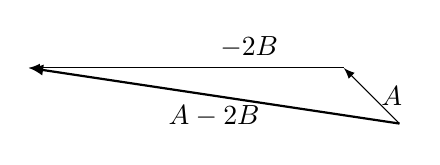
\begin{tikzpicture}
\pgfmathsetmacro{\a}{135}
\pgfmathsetmacro{\b}{1}
\pgfmathsetmacro{\aa}{0}
\pgfmathsetmacro{\bb}{2}
\pgfmathsetmacro{\aaa}{90}
\pgfmathsetmacro{\bbb}{1}
\draw[-latex](0,0)--(\a:\b)node[pos=0.5,right]{$A$};
\draw[-latex](\a:\b)--++(\aa:-2*\bb)coordinate(ka)node[pos=0.3,above]{$-2B$};
\draw[thick,-latex](0,0)--(ka)coordinate(kb)node[pos=0.5,below]{$A-2B$};
\end{tikzpicture}
\caption{}
\end{subfigure}%
\begin{subfigure}{0.45\textwidth}
\centering
\begin{tikzpicture}
\pgfmathsetmacro{\a}{135}
\pgfmathsetmacro{\b}{1}
\pgfmathsetmacro{\aa}{0}
\pgfmathsetmacro{\bb}{2}
\pgfmathsetmacro{\aaa}{90}
\pgfmathsetmacro{\bbb}{1}
\draw[-latex](0,0)--(\a:1/2*\b)node[pos=0.5,above right]{$\tfrac{1}{2}A$};
\draw[-latex](\a:1/2*\b)--++(\aaa:-\bbb)coordinate(ka)node[pos=0.3,left]{$-C$};
\draw[thick,-latex](0,0)--(ka)coordinate(kb)node[pos=0.5,right]{$\tfrac{1}{2}A-C$};
\end{tikzpicture}
\caption{}
\end{subfigure}
\caption{}
\label{شکل_سوال_سمتیہ_جوابات_چند_جمع_منفی}
\end{figure}
سوال \حوالہ{سوال_سمتیہ_مجموعات_الف} تا سوال \حوالہ{سوال_سمتیہ_مجموعات_ب} میں \عددی{\kvec{A}=2\ai-7\aj}، \عددی{\kvec{B}=\ai+6\aj} اور \عددی{\kvec{C}=\sqrt{3}\ai-\pi\aj} لیں۔ نتائج کو \عددی{a\ai+b\aj} روپ میں لکھیں۔

\ابتدا{سوال}\شناخت{سوال_سمتیہ_مجموعات_الف}
$\kvec{A}+2\kvec{B}$\\
جواب:\quad
$4\ai+5\aj$
\انتہا{سوال}
%====================
\ابتدا{سوال}
$\kvec{A}+\kvec{B}-\kvec{C}$
\انتہا{سوال}
%====================
\ابتدا{سوال}
$3\kvec{A}-\frac{1}{\pi}\kvec{C}$\\
جواب:\quad
$(6-\tfrac{\sqrt{3}}{\pi})\ai-20\aj$
\انتہا{سوال}
%====================
\ابتدا{سوال}\شناخت{سوال_سمتیہ_مجموعات_ب}
$2\kvec{A}-3\kvec{B}+32\aj$
\انتہا{سوال}
%====================
\ابتدا{سوال}\شناخت{سوال_سمتیہ_پ}
مثلث \عددی{ABC}  کے اضلاع سمتیات \عددی{\kvec{u}}، \عددی{\kvec{v}} اور \عددی{\kvec{w}} دیتے ہیں (شکل \حوالہ{شکل_سوال_سمتیہ_پ})۔
\begin{enumerate}[a.]
\item
\عددی{\kvec{w}} کو \عددی{\kvec{u}} اور \عددی{\kvec{v}} کی صورت میں لکھیں۔
\item
\عددی{\kvec{v}} کو \عددی{\kvec{u}} اور \عددی{\kvec{w}} کی صورت میں لکھیں۔
\end{enumerate}
جواب:\quad
(ا) \عددی{\kvec{w}=\kvec{v}+\kvec{u}} (ب) \عددی{\kvec{v}=\kvec{w}-\kvec{u}}
\انتہا{سوال}
%===================
\ابتدا{سوال}\شناخت{سوال_سمتیہ_ت}
مثلث \عددی{ABC} کے اضلاع  سمتیات \عددی{\kvec{u}} اور \عددی{\kvec{w}} دیتے ہیں جبکہ \عددی{BC} کا وسطی نقطہ \عددی{N} ہے (شکل \حوالہ{شکل_سوال_سمتیہ_ت})۔ سمتیہ \عددی{\kvec{a}} کو \عددی{\kvec{u}} اور \عددی{\kvec{w}} کی صورت میں لکھیں۔
\انتہا{سوال}
%==================

سوال \حوالہ{سوال_سمتیہ_نقطہ_الف} تا سوال \حوالہ{سوال_سمتیہ_نقطہ_ٹ} میں سمتیہ کو \عددی{a\ai+b\aj} روپ میں لکھیں۔ محددی سطح پر مبدا سے شروع کرتے ہوئے  انہیں ترسیم کریں۔

\ابتدا{سوال}\شناخت{سوال_سمتیہ_نقطہ_الف}
نقاط \عددی{N_1(5,7)} اور \عددی{N_2(2,9)} کے بیچ قطع \عددی{\krightharpoonup{N_1N_2}} تلاش کریں۔\\
جواب:\quad
شکل \حوالہ{شکل_سوال_سمتیہ_نقطہ_الف}
\انتہا{سوال}
%======================
\ابتدا{سوال}
نقاط \عددی{N_1(1,2)} اور \عددی{N_2(-3,5)} کے بیچ قطع \عددی{\krightharpoonup{N_1N_2}}  تلاش کریں۔
\انتہا{سوال}
%======================
\ابتدا{سوال}\شناخت{سوال_سمتیہ_نقطہ_ب}
نقاط \عددی{A(-5,3)} اور \عددی{B(-10,8)} کے بیچ قطع \عددی{\krightharpoonup{AB}}  تلاش کریں۔\\
جواب:\quad
شکل \حوالہ{شکل_سوال_سمتیہ_نقطہ_ب}
\انتہا{سوال}
%======================
\ابتدا{سوال}
نقاط \عددی{A(-7,-8)} اور \عددی{B(6,11)} کے بیچ قطع \عددی{\krightharpoonup{AB}}  تلاش کریں۔
\انتہا{سوال}
%======================
\ابتدا{سوال}\شناخت{سوال_سمتیہ_نقطہ_پ}
نقاط \عددی{N_1(1,3)} اور \عددی{N_2(2,-1)} کے بیچ قطع \عددی{\krightharpoonup{N_1N_2}}  تلاش کریں۔\\
جواب:\quad
شکل \حوالہ{شکل_سوال_سمتیہ_نقطہ_پ}
\انتہا{سوال}
%======================
\ابتدا{سوال}
نقاط \عددی{N_3(1,3)} اور \عددی{N_4} کے بیچ قطع \عددی{\krightharpoonup{N_3N_4}}  تلاش کریں جہاں \عددی{N_1(2,-1)} اور \عددی{N_2(-4,3)} کو ملانے والے قطع کا وسطی نقطہ \عددی{N_4} ہے۔
\انتہا{سوال}
%======================
\ابتدا{سوال}\شناخت{سوال_سمتیہ_نقطہ_ت}
نقاط \عددی{A(1,-1)}، \عددی{B(2,0)}، \عددی{C(-1,3)} اور \عددی{D(-2,2)} دیے گئے ہیں۔ سمتیات \عددی{\krightharpoonup{CD}} اور \عددی{\krightharpoonup{AB}} کا مجموعہ تلاش کریں۔\\
جواب:\quad
شکل \حوالہ{شکل_سوال_سمتیہ_نقطہ_ت}
\انتہا{سوال}
%==================
\ابتدا{سوال}\شناخت{سوال_سمتیہ_نقطہ_ٹ}
نقطہ \عددی{A} سے مبدا تک سمتیہ، جہاں \عددی{\krightharpoonup{AB}=4\ai-2\aj} اور \عددی{B(-2,5)} ہیں۔
\انتہا{سوال}
%=====================
\ابتدا{سوال}
سمتیہ \عددی{\krightharpoonup{AB}=3\ai-\aj} اور نقطہ \عددی{A(2,9)} دیا گیا ہے۔نقطہ \عددی{B} تلاش کریں۔\\
جواب:\quad
$(5,8)$
\انتہا{سوال}
%=======================
\ابتدا{سوال}
سمتیہ \عددی{\krightharpoonup{NQ}=-6\ai-4\aj} اور نقطہ \عددی{Q(3,3)} دیا گیا ہے۔نقطہ \عددی{N} تلاش کریں۔
\انتہا{سوال}
%====================
\begin{figure}
\centering
\begin{minipage}{0.22\textwidth}
\centering
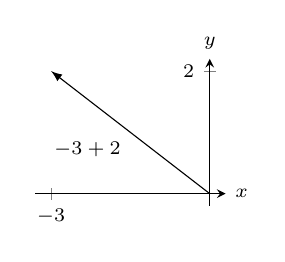
\begin{tikzpicture}[font=\scriptsize]
\begin{axis}[width=4cm,axis lines=middle,xlabel={$x$},ylabel={$y$},xlabel style={at={(current axis.right of origin)},anchor=west},ylabel style={at={(current axis.above origin)},anchor=south},xtick={-3},ytick={2},enlargelimits=true]
\addplot[-latex] plot coordinates {(0,0)(-3,2)}node[pos=0.5,below left]{$-3\ai+2\aj$};
\end{axis}
\end{tikzpicture}
\caption{}
\label{شکل_سوال_سمتیہ_نقطہ_الف}
\end{minipage}\hfill
\begin{minipage}{0.22\textwidth}
\centering
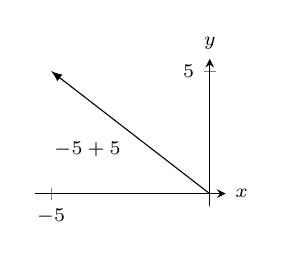
\begin{tikzpicture}[font=\scriptsize]
\begin{axis}[width=4cm,axis lines=middle,xlabel={$x$},ylabel={$y$},xlabel style={at={(current axis.right of origin)},anchor=west},ylabel style={at={(current axis.above origin)},anchor=south},xtick={-5},ytick={5},enlargelimits=true]
\addplot[-latex] plot coordinates {(0,0)(-5,5)}node[pos=0.5,below left]{$-5\ai+5\aj$};
\end{axis}
\end{tikzpicture}
\caption{}
\label{شکل_سوال_سمتیہ_نقطہ_ب}
\end{minipage}\hfill
\begin{minipage}{0.22\textwidth}
\centering
\begin{tikzpicture}[font=\scriptsize]
\begin{axis}[width=4cm,axis lines=middle,xlabel={$x$},ylabel={$y$},xlabel style={at={(current axis.right of origin)},anchor=west},ylabel style={at={(current axis.above origin)},anchor=south},xtick={1},ytick={-4},enlargelimits=true]
\addplot[-latex] plot coordinates {(0,0)(1,-4)}node[pos=0.5,below left]{$\ai-4\aj$};
\end{axis}
\end{tikzpicture}
\caption{}
\label{شکل_سوال_سمتیہ_نقطہ_پ}
\end{minipage}\hfill
\begin{minipage}{0.22\textwidth}
\centering
\begin{tikzpicture}[font=\scriptsize]
\begin{axis}[clip=false,width=4cm,axis lines=middle,xlabel={$x$},ylabel={$y$},xlabel style={at={(current axis.right of origin)},anchor=west},ylabel style={at={(current axis.above origin)},anchor=south},xtick={-1,1},ytick={-1,1},enlargelimits=true]
\addplot[-latex] plot coordinates {(0,0)(1,1)}node[above left]{$\krightharpoonup{AB}$};
\addplot[-latex] plot coordinates {(0,0)(-1,-1)}node[below right]{$\krightharpoonup{CD}$};
\addplot[]plot coordinates {(0,0)}node[circ]{}node[pin={[font=\tiny,pin distance=0.1cm]135:{$\krightharpoonup{AB}+\krightharpoonup{CD}=0$}}]{};
\end{axis}
\end{tikzpicture}
\caption{}
\label{شکل_سوال_سمتیہ_نقطہ_ت}
\end{minipage}
\end{figure}
\موٹا{اکائی سمتیات}\\
سوال \حوالہ{سوال_سمتیہ_اکائی_الف} تا سوال \حوالہ{سوال_سمتیہ_اکائی_پ} میں دیے سمتیات ترسیم کریں۔ ان سمتیات کو \عددی{a\ai+b\aj} روپ میں لکھیں۔

\ابتدا{سوال}\شناخت{سوال_سمتیہ_اکائی_الف}
زاویہ \عددی{\theta=\tfrac{\pi}{6}} اور \عددی{\theta=\tfrac{2\pi}{3}} کے لئے اکائی سمتیات \عددی{\kvec{u}=(\cos\theta)\ai+(\sin\theta)\aj} ترسیم کریں۔ دائرہ \عددی{x^2+y^2=1} کی ترسیم بھی شامل کریں۔\\
جواب:\quad
شکل \حوالہ{شکل_سوال_سمتیہ_اکائی_الف}
\انتہا{سوال}
%===================
\ابتدا{سوال}
زاویہ \عددی{\theta=-\tfrac{\pi}{4}} اور \عددی{\theta=-\tfrac{3\pi}{4}} کے لئے اکائی سمتیات \عددی{\kvec{u}=(\cos\theta)\ai+(\sin\theta)\aj} ترسیم کریں۔ دائرہ \عددی{x^2+y^2=1} کی ترسیم بھی شامل کریں۔
\انتہا{سوال}
%======================
\ابتدا{سوال}\شناخت{سوال_سمتیہ_اکائی_ب}
سمتیہ \عددی{\aj} کو مبدا کے گرد گھڑی کے الٹ رخ \عددی{\tfrac{3\pi}{4}} ریڈیئن  گھما کر حاصل اکائی سمتیہ ترسیم کریں۔\\
جواب:\quad
شکل \حوالہ{شکل_سوال_سمتیہ_اکائی_ب}
\انتہا{سوال}
%===================
\ابتدا{سوال}\شناخت{سوال_سمتیہ_اکائی_پ}
سمتیہ \عددی{\aj} کو مبدا کے گرد گھڑی کے رخ \عددی{\tfrac{2\pi}{3}} ریڈیئن  گھما کر حاصل اکائی سمتیہ ترسیم کریں۔
\انتہا{سوال}
%===================
\begin{figure}
\centering
\begin{minipage}{0.22\textwidth}
\centering
\begin{tikzpicture}[font=\tiny]
\begin{axis}[clip=false,axis equal,width=4cm,axis lines=middle,xlabel={$x$},ylabel={$y$},xlabel style={at={(current axis.right of origin)},anchor=west},ylabel style={at={(current axis.above origin)},anchor=south},xtick={1},ytick={\empty},enlargelimits=true]
\addplot[-latex,thick,data cs=polar]plot coordinates{(0,0)(30,1)}node[above,xshift=2ex,yshift=1ex]{$\kvec{u}=\tfrac{\sqrt{3}}{2}\ai+\tfrac{1}{2}\aj$};
\addplot[-latex,thick,data cs=polar]plot coordinates{(0,0)(120,1)}node[above,xshift=-3ex]{$\kvec{u}=-\tfrac{1}{2}\ai+\tfrac{\sqrt{3}}{2}\aj$};
\addplot[domain=0:360]({1*cos(x)},{1*sin(x)});
\addplot[-stealth,domain=0:30]({0.5*cos(x)},{0.5*sin(x)})node[pos=0.6,right]{$\tfrac{\pi}{6}$};
\addplot[-stealth,domain=0:120]({0.3*cos(x)},{0.3*sin(x)})node[pos=0.5,above]{$\tfrac{2\pi}{3}$};
\end{axis}
\end{tikzpicture}
\caption{}
\label{شکل_سوال_سمتیہ_اکائی_الف}
\end{minipage}\hfill
\begin{minipage}{0.22\textwidth}
\centering
\begin{tikzpicture}[font=\tiny]
\pgfmathsetmacro{\k}{-1/sqrt(2)}
\begin{axis}[clip=false,axis equal,width=4cm,axis lines=middle,xlabel={$x$},ylabel={$y$},xlabel style={at={(current axis.right of origin)},anchor=west},ylabel style={at={(current axis.above origin)},anchor=south},xtick={\k},ytick={\k},xticklabels={$-\tfrac{\sqrt{2}}{2}$},yticklabels={$-\tfrac{\sqrt{2}}{2}$},enlargelimits=true]
\addplot[-latex]plot coordinates {(0,0)(\k,\k)}node[pos=0.5,left]{$-\tfrac{\sqrt{2}}{2}\ai-\tfrac{\sqrt{2}}{2}\aj$};
\end{axis}
\end{tikzpicture}
\caption{}
\label{شکل_سوال_سمتیہ_اکائی_ب}
\end{minipage}\hfill
\begin{minipage}{0.22\textwidth}
\centering
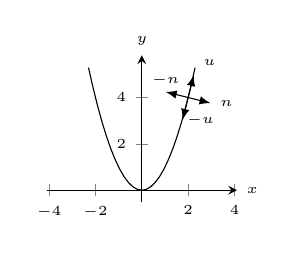
\begin{tikzpicture}[font=\tiny,declare function={f(\x)=(\x)^2;}]
\pgfmathsetmacro{\k}{1/sqrt(17)}
\begin{axis}[clip=false,axis equal,width=4cm,axis lines=middle,xlabel={$x$},ylabel={$y$},xlabel style={at={(current axis.right of origin)},anchor=west},ylabel style={at={(current axis.above origin)},anchor=south},enlargelimits=true]
\addplot[domain=-2.3:2.3]{f(x)};
\draw[-latex] (axis cs:2,4)--(axis cs:2+\k,4+4*\k)node[above right]{$\kvec{u}$};
\draw[-latex] (axis cs:2,4)--(axis cs:2-\k,4-4*\k)node[xshift=1.5ex]{$-\kvec{u}$};
\draw[-latex] (axis cs:2,4)--(axis cs:2+4*\k,4-\k)node[right]{$\kvec{n}$};
\draw[-latex] (axis cs:2,4)--(axis cs:2-4*\k,4+\k)node[yshift=1ex]{$-\kvec{n}$};
\end{axis}
\end{tikzpicture}
\caption{}
\label{شکل_سوال_سمتیہ_عمودی_مماسی_الف}
\end{minipage}\hfill
\begin{minipage}{0.22\textwidth}
\centering
\begin{tikzpicture}[font=\tiny,declare function={f(\x)=rad(atan(\x));}]
\pgfmathsetmacro{\k}{2/sqrt(5)}
\pgfmathsetmacro{\a}{pi/4}
\begin{axis}[clip=false,width=4cm,axis lines=middle,xlabel={$x$},ylabel={$y$},xlabel style={at={(current axis.right of origin)},anchor=west},ylabel style={at={(current axis.above origin)},anchor=south},enlargelimits=true, xtick={1},ytick={\a},yticklabels={$\tfrac{\pi}{4}$}]
\addplot[smooth,samples=100,domain=-1:2.5]{f(x)}node[below]{$y=\tan^{-1}(x)$};
\addplot[-latex] plot coordinates {(1,pi/4)(1+\k,pi/4+1/2*\k)}node[above]{$\kvec{u}$};
\addplot[-latex] plot coordinates {(1,pi/4)(1-\k,pi/4-1/2*\k)}node[left]{$-\kvec{u}$};
\addplot[-latex] plot coordinates {(1,pi/4)(1+1/2*\k,pi/4-\k)}node[below]{$\kvec{n}$};
\addplot[-latex] plot coordinates {(1,pi/4)(1-1/2*\k,pi/4+\k)}node[above]{$-\kvec{n}$};
\end{axis}
\end{tikzpicture}
\caption{}
\label{شکل_سوال_سمتیہ_عمودی_مماسی_ب}
\end{minipage}
\end{figure}
%==========================
سوال \حوالہ{سوال_سمتیہ_اکائی_گھوم_الف} اور سوال \حوالہ{سوال_سمتیہ_اکائی_گھوم_ب} میں اکائی سمتیہ \عددی{\kvec{u}=(\cos\theta)\ai+(\sin\theta)\aj} اسی رخ تلاش کریں۔

\ابتدا{سوال}\شناخت{سوال_سمتیہ_اکائی_گھوم_الف}
$6\ai-8\aj$\\
جواب:\quad
$\tfrac{3}{5}\ai-\tfrac{4}{5}\aj$
\انتہا{سوال}
%==================
\ابتدا{سوال}\شناخت{سوال_سمتیہ_اکائی_گھوم_ب}
$-\ai+3\aj$
\انتہا{سوال}
%=====================

سوال \حوالہ{سوال_سمتیہ_عمودی_مماسی_الف} تا سوال \حوالہ{سوال_سمتیہ_عمودی_مماسی_پ} میں دیے گئے نقطہ پر منحنی کے مماسی اکائی سمتیات اور عمودی اکائی سمتیات تلاش کریں۔ منحنی اور اکائی سمتیات کو ایک ساتھ ترسیم کریں۔ (سمتیات کی تعداد چار ہو گی۔)

\ابتدا{سوال}\شناخت{سوال_سمتیہ_عمودی_مماسی_الف}
$y=x^2,\quad (2,4)$\\
جواب:\quad
$\kvec{u}=\tfrac{1}{\sqrt{17}}\ai+\tfrac{4}{\sqrt{17}}\aj,\quad -\kvec{u}=-\tfrac{1}{\sqrt{17}}\ai-\tfrac{4}{\sqrt{17}}\aj,$\\
$ \kvec{n}=\tfrac{4}{\sqrt{17}}\ai-\tfrac{1}{\sqrt{17}}\aj,\quad -\kvec{n}=-\tfrac{4}{\sqrt{17}}\ai+\tfrac{1}{\sqrt{17}}\aj$\quad
شکل \حوالہ{شکل_سوال_سمتیہ_عمودی_مماسی_الف}
\انتہا{سوال}
%======================
\ابتدا{سوال}
$x^2+2y^2=6,\quad (2,1)$
\انتہا{سوال}
%======================
\ابتدا{سوال}\شناخت{سوال_سمتیہ_عمودی_مماسی_ب}
$y=\tan^{-1}x,\quad (1,\tfrac{\pi}{4})$\\
جواب:\quad
$\kvec{u}=\tfrac{1}{\sqrt{5}}(2\ai+\aj),\quad -\kvec{u}=\tfrac{1}{\sqrt{5}}(-2\ai-\aj),$\\
$\kvec{n}=\tfrac{1}{\sqrt{5}}(-\ai+2\aj),\quad -\kvec{n}=\tfrac{1}{\sqrt{5}}(\ai-2\aj),$\quad 
شکل \حوالہ{شکل_سوال_سمتیہ_عمودی_مماسی_ب}
\انتہا{سوال}
%======================
\ابتدا{سوال}\شناخت{سوال_سمتیہ_عمودی_مماسی_پ}
$y=\sum_{n=0}^{\infty}\frac{x^n}{n!},\quad (0,1)$
\انتہا{سوال}
%======================
سوال \حوالہ{سوال_سمتیہ_عمودی_مماسی_نقطہ_الف} تا سوال \حوالہ{سوال_سمتیہ_عمودی_مماسی_نقطہ_ب} میں دیے گئے نقطہ پر منحنی کے مماسی اور عمودی اکائی سمتیات تلاش کریں۔ 

\ابتدا{سوال}\شناخت{سوال_سمتیہ_عمودی_مماسی_نقطہ_الف}
$3x^2+8xy+2y^2-3=0,\quad (1,0)$\\
جواب:\quad
$\kvec{u}=\pm\tfrac{1}{5}(-4\ai+3\aj),\quad \kvec{v}=\pm\tfrac{1}{5}(3\ai+4\aj)$
\انتہا{سوال}
%=====================
\ابتدا{سوال}
$x^2-6xy+8y^2-2x-1=0,\quad (1,1)$
\انتہا{سوال}
%=====================
\ابتدا{سوال}
$y=\int_{0}^{x}\sqrt{3+t^4}\dif t,\quad (0,0)$\\
جواب:\quad
$\kvec{u}=\pm\tfrac{1}{2}(\ai+\sqrt{3}\aj),\quad \kvec{v}=\pm\tfrac{1}{2}(-\sqrt{3}\ai+\aj)$
\انتہا{سوال}
%=====================
\ابتدا{سوال}\شناخت{سوال_سمتیہ_عمودی_مماسی_نقطہ_ب}
$y=\int_{e}^{x}\ln (\ln t)\dif t,\quad (e,0)$
\انتہا{سوال}
%=====================

\موٹا{لمبائی اور رخ}\\
سوال \حوالہ{سوال_سمتیہ_لمبائی_رخ_الف} اور سوال \حوالہ{سوال_سمتیہ_لمبائی_رخ_ب} میں دیے سمتیہ کو لمبائی ضرب رخ کی صورت میں لکھیں۔

\ابتدا{سوال}\شناخت{سوال_سمتیہ_لمبائی_رخ_الف}
$5\ai+12\aj$\\
جواب:\quad
$13(\tfrac{5}{13}\ai+\tfrac{12}{13}\aj)$
\انتہا{سوال}
%====================
\ابتدا{سوال}\شناخت{سوال_سمتیہ_لمبائی_رخ_ب}
$2\ai-3\aj$
\انتہا{سوال}
%====================
\ابتدا{سوال}
سمتیہ \عددی{3\ai-4\aj} کے متوازی دو اکائی سمتیات دریافت کریں۔\\
جواب:\quad
$\tfrac{3}{5}\ai-\tfrac{4}{5}\aj,\quad -\tfrac{3}{5}\ai+\tfrac{4}{5}\aj$
\انتہا{سوال}
%=======================
\ابتدا{سوال}
سمتیہ \عددی{\kvec{A}=-\ai+2\aj} کے مخالف رخ ایسا سمتیہ تلاش کریں جس کی لمبائی \عددی{2} ہو۔ ایسے کتنے سمتیات ممکن ہیں؟
\انتہا{سوال}
%=========================
\ابتدا{سوال}
دکھائیں کہ \عددی{\kvec{A}=3\ai+6\j} اور \عددی{\kvec{B}=-\ai-2\aj} ایک دوسرے کے مخالف رخ ہیں۔ دونوں کا خاکہ بنائیں۔
\انتہا{سوال}
%=======================
\ابتدا{سوال}
دکھائیں کہ \عددی{\kvec{A}=3\ai+6\j} اور \عددی{\kvec{B}=\tfrac{1}{2}\ai+\aj} کے رخ ایک دوسرے جیسے ہیں۔
\انتہا{سوال}
%=======================

\موٹا{نظریہ اور مثالیں}\\
\ابتدا{سوال}
آپ ایک ریڑھی کو قوت \عددی{\kvec{F}} سے کھینچ رہے ہیں جس کی مقدار \عددی{\abs{\kvec{F}}=\SI{10}{\newton}} ہے۔زمین کے ساتھ قوت کا زاویہ \عددی{30^{\circ}} ہے۔ اس قوت کے \عددی{x} اور \عددی{y} اجزاء تلاش کریں۔\\
جواب:\quad
$5\sqrt{3}\ai,\quad 5\aj$
\انتہا{سوال}
%===================
\ابتدا{سوال}
پتنگ کی ڈوری آپ کو زمین کے ساتھ \عددی{45^{\circ}} زاویہ پر \عددی{\SI{5}{\newton}} قوت سے کھینچتی ہے۔ اس قوت کے افقی اور انتصابی اجزاء تلاش کریں۔
\انتہا{سوال}
%===============
\ابتدا{سوال}\شناخت{سوال_سمتیہ_سمتیات_دیگر}
سمتیہ \عددی{\kvec{A}=2\ai+\aj}، \عددی{\kvec{B}=\ai+\aj} اور \عددی{\kvec{C}=\ai-\aj} دیے گئے ہیں۔ ایسے غیر سمتیات \عددی{\alpha} اور \عددی{\beta} کہ \عددی{\kvec{A}=\alpha\kvec{B}+\beta\kvec{C}} ہو۔\\
جواب:\quad
$\alpha=\tfrac{3}{2},\quad \beta=\tfrac{1}{2}$
\انتہا{سوال}
%=================
\ابتدا{سوال}
سمتیات \عددی{\kvec{A}=\ai-2\aj}، \عددی{\kvec{B}=2\ai+3\aj} اور \عددی{\kvec{C}=\ai+\aj} دیے گئے ہیں۔ سمتیہ \عددی{\kvec{A}=\kvec{A}_1+\kvec{A}_2} لکھیں جہاں \عددی{\kvec{A}_1} سمتیہ \عددی{\kvec{B}} کے متوازی اور \عددی{\kvec{A}_2} سمتیہ \عددی{\kvec{C}} کے متوازی ہے۔ (سوال \حوالہ{سوال_سمتیہ_سمتیات_دیگر} دیکھیں۔)
\انتہا{سوال}
%====================
\ابتدا{سوال}
 ایک پرندہ اپنے گھونسلے سے اڑ کر، مشرق سے شمال کی طرف \عددی{60^{\circ}} پر  \عددی{5} کلومیٹر دور ایک درخت پر آرام کے لئے بیٹھتا ہے۔ اس کے بعد یہ جنوب مشرق رخ \عددی{10} کلومیٹر دور ایک کھنبے پر اڑ کر  بیٹھتا ہے۔ مستوی \عددی{xy} کے مبدا پر گھونسلا، مثبت \عددی{x} محور پر مشرق اور مثبت \عددی{y} محور پر شمال  رکھ (ا) درخت کا مقام تلاش کریں۔ (ب) کھنبے کا مقام تلاش کریں۔\\
جواب:\quad
(ا) \عددی{(5\cos 60^{\circ},5\sin 60^{\circ})=(\tfrac{5}{2},\tfrac{5\sqrt{3}}{2}}،\\
 (ب) \عددی{(5\cos 60^{}+10\cos 315^{},5\sin 60^{\circ}+10\sin 315^{\circ})=(\tfrac{5+\sqrt{2}}{2},\tfrac{5\sqrt{3}-10\sqrt{2}}{2})}
\انتہا{سوال}
%===================
\ابتدا{سوال}
 ایک پرندہ اپنے گھونسلے سے اڑ کر، شمال مشرق رخ \عددی{7} کلومیٹر دور ایک درخت پر آرام کرتا ہے۔ اس کے بعد یہ مغرب سے  \عددی{30^{\circ}} زاویہ جنوب کے رخ \عددی{8} کلومیٹر دور ایک کھنبے پر اڑ کر بیٹھتا ہے۔ مستوی \عددی{xy} کے مبدا پر گھونسلا، مثبت \عددی{x} محور پر مشرق اور مثبت \عددی{y} محور پر شمال  رکھ (ا) درخت کا مقام تلاش کریں۔ (ب) کھنبے کا مقام تلاش کریں۔
\انتہا{سوال}
%===================
\ابتدا{سوال}
مستوی میں \عددی{\kvec{v}} ایک سمتیہ ہے جو \عددی{y} محور کے متوازی نہیں ہے۔ سمتیہ \عددی{\kvec{v}} کی ڈھلوان اور سمتیہ \عددی{-\kvec{v}} کی ڈھلوان کا آپس میں کیا تعلق ہو گا؟ اپنے جواب کی وجہ پیش کریں۔\\
جواب:\quad
\عددی{-\kvec{v}=-a\ai-b\aj} کی ڈھلوان \عددی{\tfrac{(-b)}{(-a)}} ہے۔ یہی \عددی{\kvec{v}} کی بھی ڈھلوان ہے۔
\انتہا{سوال}
%==============

\begin{figure}
\centering
\begin{minipage}{0.4\textwidth}
\centering
\begin{tikzpicture}[font=\small,x={(-0.5cm,-0.5cm)},y={(1cm,0cm)},z={(0cm,1cm)}]
\pgfmathsetmacro{\a}{1}
\pgfmathsetmacro{\b}{1.5}
\pgfmathsetmacro{\c}{1.2}
\draw[-latex](0,0,0)node[below]{$O$}--(\a+0.75,0,0)node[below]{$x$};
\draw[-latex](0,0,0)--(0,\b+1,0)node[below]{$y$};
\draw[-latex](0,0,0)--(0,0,\c+0.75)node[above]{$z$};
\draw[opacity=0.5,fill=gray](\a,0,0)--++(0,\b,0)--++(0,0,\c)--++(0,-\b,0)--++(0,0,-\c);
\draw[opacity=0.5,fill=gray](\a,\b,0)--++(-\a,0,0)--++(0,0,\c)--++(\a,0,0)--++(0,0,-\c);
\draw[opacity=0.5,fill=gray](\a,0,\c)--++(0,\b,0)--++(-\a,0,0)--++(0,-\b,0)--++(\a,0,0);
\draw(\a,0,0)node[left]{$(x,0,0)$};
\draw(0,\b,0)node[above right]{$(0,y,0)$};
\draw(0,0,\c)node[left]{$(0,0,z)$};
\draw(\a,0.75*\b,0.1*\c) to [out=-135,in=90]++(0.25,-0.25,-0.25)node[below]{$x=$مستقل};
\draw(0.1*\a,0.5*\b,\c) to [out=45,in=-135]++(-0.25,0.25,0.25)node[above]{$z=$مستقل};
\draw(0.1*\a,\b,0.7*\c) to [out=45,in=180]++(0.25,0.5,0.25)node[right]{$y=$مستقل};
\draw(\a,\b,0)node[right]{$(x,y,0)$};
\draw(0,\b,\c)node[right,yshift=1ex]{$(0,y,z)$};
\draw(\a,0,\c)node[left]{$(x,0,z)$};
\end{tikzpicture}
\caption{دایاں ہاتھ کارتیسی نظام۔}
\label{شکل_سمتیہ_دایاں_کارتیسی_نظام}
\end{minipage}\hfill
\begin{minipage}{0.55\textwidth}
\centering
\begin{tikzpicture}[font=\small,x={(-0.5cm,-0.5cm)},y={(1cm,0cm)},z={(0cm,1cm)}]
\pgfmathsetmacro{\xc}{2}
\pgfmathsetmacro{\xh}{2.5}
\pgfmathsetmacro{\xl}{0}
\pgfmathsetmacro{\yc}{1.75}
\pgfmathsetmacro{\yh}{2.5}
\pgfmathsetmacro{\yl}{0}
\pgfmathsetmacro{\zc}{2}
\pgfmathsetmacro{\zh}{2.5}
\pgfmathsetmacro{\zl}{0}

\coordinate (xa) at (\xc,\yl,\zl);
\coordinate (xb) at (\xc,\yl,\zh);
\coordinate (xc) at (\xc,\yh,\zh);
\coordinate (xd) at (\xc,\yh,\zl);

\coordinate (ya) at (\xh,\yc,\zl);
\coordinate (yb) at (\xh,\yc,\zh);
\coordinate (yc) at (\xl,\yc,\zh);
\coordinate (yd) at (\xl,\yc,\zl);

\coordinate (za) at (\xh,\yl,\zc);
\coordinate (zb) at (\xl,\yl,\zc);
\coordinate (zc) at (\xl,\yh,\zc);
\coordinate (zd) at (\xh,\yh,\zc);

%==========
\path [name path={x}]  (xa) -- (xb)--(xc)--(xd)--cycle;
\path [name path={y}]  (ya) -- (yb)--(yc)--(yd)--cycle;
\path [name path={z}]  (za) -- (zb)--(zc)--(zd)--cycle;
%dashed intersections
\path [name path={xy},name intersections={of=x and y, by={xy1, xy2, xy3,xy4}}](xy1)--(xy4);
\path [name path={xz},name intersections={of=x and z, by={xz1, xz2, xz3,xz4}}] (xz4) -- (xz1);
\path [name path={yz},name intersections={of=y and z, by={yz1, yz2, yz3,yz4}}](yz1) -- (yz3);
\path[name intersections={of=xy and xz, by={xyz}}];
%surfaces
\draw (xa)--(xb)--(xc)--(xd)--cycle;   %yz surface
\draw (ya)--(yb)--(yc)--(yd)--cycle;     %xz surface
\draw (za)--(zb)--(zc)--(zd)--cycle;     %xy surface
%hide edges
\filldraw[fill=white,fill opacity=1](za)--(xz1)--(xb)--(xy1)--(yb)--(yz1)--cycle;
\filldraw[fill=white,fill opacity=1](xy1)--(yc)--(yz3)--(zc)--(xz4)--(xc)--cycle;
\filldraw[fill=white,fill opacity=1](xd)--(xy4)--(ya)--(yz1)--(zd)--(xz4)--cycle;
%intersections
\draw[gray,dashed] (xy1)--(xyz);
\draw[gray,dashed] (xz4) -- (xyz);
\draw[gray,dashed]  (yz1) -- (xyz);
\draw[gray,dashed,shorten <=-0.5cm,name intersections={of=xz and y, by={xz_y}}](xz1) -- (xz_y)node[black,pos=0,xshift={-0.5cm},left]{\RL{خط $x=2,\,z=5$}};
\draw[gray,dashed,shorten <=-0.75cm,name intersections={of=yz and x, by={yz_x}}](yz3) -- (yz_x)node[black,yshift=1cm,above right]{\RL{خط $y=3,\, z=5$}};
\draw[gray,dashed,shorten <=-0.5cm,name intersections={of=xy and z, by={xy_z}}](xy4) -- (xy_z)node[pos=0,yshift=-0.5cm,black,below]{\RL{خط $x=2,\, y=3$}};
%axis
\draw[lgray](0,0,0)--(\xc,0,0) node[circ]{}node [black,left]{$(2,0,0)$};
\draw[lgray](0,0,0)--(0,\yc,0)node[circ]{}node[black,below,xshift=3ex]{$(0,3,0)$};
\draw[lgray](0,0,0)--(0,0,\zc)node[circ]{}node[black,left]{$(0,0,5)$};
\draw[gray](\xc,0,0)--(3,0,0)node[left]{$x$};
\draw[gray](0,\yc,0)--(0,3,0)node[right]{$y$};
\draw[gray](0,0,\zc)--(0,0,3)node[right]{$z$};
%text
\draw[<-] ($(xa)!0.2!(xb)$) to [out=150,in=-10]++(0,-0.5,0.5)node[black,left]{\RL{سطح $x=2$}};
\draw[gray,<-] ($(yd)!0.2!(yc)$) to [out=10,in=150]++(0,0.5,0.5)node[black,right]{\RL{سطح $y=3$}};
\draw[gray,<-](zc) to [out=20,in=-150]++(0,0.5,0.25)node[right,black]{\RL{سطح $z=5$}};
%\draw[gray,<-] ($(xy4)!0.2!(xy1)$) to [out=-10,in=150]++(0,1,-0.5)node[black,right,align=right]{\RL{$x=2$ اور $y=3$ سطحیں }\\ \RL{اس لکیر پر آپس میں ملتی ہیں}};
\draw[fill] (xyz) circle (1pt);
\draw[gray,<-]  (xyz)++(0,0.1,0.1) to [out=20,in=180] ++(0,2,0.5) node[right,black] {$(2,3,5)$};
\end{tikzpicture}%
\caption{سطح \عددی{x=2}، \عددی{y=3} اور \عددی{z=5} نقطہ \عددی{(2,3,5)} سے گزرتی تین خط تعین کرتے ہیں۔}
\label{شکل_سمتیہ_تین_سطحیں_لکیروں_پر_ملتی_ہیں}
\end{minipage}
\end{figure}
\حصہ{کارتیسی (مستطیل) محدد اور فضا میں سمتیات}
ہم اب سہ بعدی کارتیسی محدد بیان کرتے ہیں اور فضا میں اپنا راستہ تلاش کرنا سیکھتے ہیں۔ ہم فاصلہ کی تعریف جانیں گے،  فضا میں سمتیات کے ساتھ کام کرنا (مستوی کے قواعد اب بھی لاگو ہوں گے، پس اب ایک محدد بڑھ جائے گا)، اور نقطوں کے سلسلہ کا مساوات اور عدم مساوات کے ساتھ تعلق سیکھیں گے۔

\جزوحصہء{کارتیسی محدد} 
فضا میں نقطہ کی تلاش کے لئے تین آپس میں عمودی محددی محور استعمال کیے جاتے ہیں۔  شکل \حوالہ{شکل_سمتیہ_دایاں_کارتیسی_نظام} میں محور \عددی{Ox}، \عددی{Oy} اور \عددی{Oz} دایاں ہاتھ محددی نظام دیتے ہیں۔ دائیں ہاتھ کے نظام میں، انگوٹھے کو باقی انگلیوں کے ساتھ زاویہ قائمہ پر رکھتے ہوئے، اگر آپ اپنے دائیں ہاتھ کی چار انگلیوں کو مثبت \عددی{x} محور پر رکھ کر انہیں مثبت \عددی{y} محور کی جانب موڑیں تب آپ کا انگوٹھا مثبت \عددی{z} محور پر ہو گا۔

فضا میں نقطہ \عددی{N} سے گزرتی، محوروں کے قائمہ سطحیں ان محور کو اعداد  \عددی{(x,y,z)} پر قطع کریں گی۔ یہی اعداد نقطہ \عددی{N} کے کارتیسی محدد ہوں گے۔  

محور \عددی{x} پر نقطوں کے \عددی{y} اور \عددی{z} محدد صفر ہوں گے لہٰذا ان کے محدد کی صورت \عددی{(x,0,0)} ہو گی۔ اسی طرح محور \عددی{y} پر نقطوں کے \عددی{x} اور \عددی{z} محدد صفر ہوں گے لہٰذا ان نقطوں کے محدد کی صورت \عددی{(0,y,0)} ہو گی۔ محور \عددی{z} پر نقطوں کے \عددی{x} اور \عددی{y} محدد صفر ہوں گے لہٰذا ان کے محددی کی صورت \عددی{(0,0,z)} ہو گی۔

محور \عددی{x} کے عمودی سطح پر تمام نقطوں کا \عددی{x} محدد وہی ہو گا جس \عددی{x} محدد  پر یہ سطح \عددی{x} محور کو قطع کرتا ہے۔ اس سطح پر نقطوں کے \عددی{y} اور \عددی{z} محدد کچھ بھی ہو سکتے ہیں۔ اسی طرح محور \عددی{y} کے عمودی سطح پر تمام نقطوں کا مشترک \عددی{y} محدد ہو گا اور  محور \عددی{z} کے عمودی سطح پر تمام نقطوں کا مشترک \عددی{z} محدد ہو گا۔ ان سطحوں کی مساوات لکھتے ہوئے ہم اس مشترکہ محدد کی قیمت لکھتے ہیں۔ یوں مستوی \عددی{x=2} محور \عددی{x} کو عمودی ہے اور یہ مستوی محور \عددی{x} کو نقطہ \عددی{x=2} پر قطع کرتا ہے۔ مستوی \عددی{y=3} محور \عددی{y} کو عمودی ہے اور اس کو نقطہ \عددی{y=3} پر قطع کرتا ہے۔مستوی \عددی{z=5} محور \عددی{z} کو عمودی ہے اور اس محور کو نقطہ \عددی{z=5} پر قطع کرتا ہے۔ شکل \حوالہ{شکل_سمتیہ_تین_سطحیں_لکیروں_پر_ملتی_ہیں} میں مستوی \عددی{x=2}، \عددی{y=3} اور \عددی{z=5} دکھائے گئے ہیں۔ ان کا مشترک نقطہ بھی دکھایا گیا ہے جہاں یہ تینوں ایک دوسرے کو قطع کرتے ہیں۔

مستوی \عددی{x=2} اور \عددی{y=3} ایک دوسرے کو ایک لکیر پر قطع کرتے ہیں (شکل \حوالہ{شکل_سمتیہ_تین_سطحیں_لکیروں_پر_ملتی_ہیں}) جو محور \عددی{z} کے متوازی ہے۔ اس لکیر کو جوڑی مساوات \عددی{x=2}، \عددی{y=3} ظاہر کرتے ہیں۔ نقطہ \عددی{(x,y,z)} صرف اور صرف اس صورت اس لکیر پر پایا جائے گا جب \عددی{x=2} اور \عددی{y=3} ہوں۔ اسی طرح مستوی \عددی{y=3} اور \عددی{z=5} ایک لکیر پر ایک دوسرے کو قطع کرتے ہیں اور اس لکیر کو جوڑی مساوات \عددی{y=3}، \عددی{z=5} ظاہر کرتے ہیں۔ یہ لکیر محور \عددی{x} کے متوازی ہو گی۔ مستوی \عددی{x=2} اور \عددی{z=5} ایک لکیر پر ایک دوسرے کو قطع کرتے ہیں اور اس لکیر کو جوڑی مساوات \عددی{x=2}، \عددی{z=5} ظاہر کرتے ہیں۔ یہ لکیر محور \عددی{y} کے متوازی ہو گی۔

محددی محوروں کے بیچ \اصطلاح{مستوی \عددی{xy}}\فرہنگ{مستوی!ایکس وائے}\حاشیہب{xy-plane}\فرہنگ{plane!xy} جس کی معیاری مساوات \عددی{z=0}؛ \اصطلاح{مستوی \عددی{yz}} جس کی معیاری مساوات \عددی{x=0}؛ اور \اصطلاح{مستوی \عددی{xz}} جس کی معیاری مساوات \عددی{y=0} ہے پائی جاتی ہیں۔ یہ تینوں مستوی مبدا \عددی{(0,0,0)} پر آپس میں ملتے ہیں (شکل \حوالہ{شکل_سمتیہ_آٹھ_ثمن})۔

تین \اصطلاح{محددی مستوی}\فرہنگ{مستوی!محددی}\حاشیہب{coordinate planes}\فرہنگ{planes!coordinate} \عددی{x=0}، \عددی{y=0} اور \عددی{z=0} فضا کو آٹھ حصوں میں تقسیم کرتے ہیں جنہیں \اصطلاح{ثُمن}\فرہنگ{ثمن}\حاشیہب{octant}\فرہنگ{octant} کہتے ہیں۔ وہ ثمن جس میں تمام محدد مثبت ہیں \اصطلاح{پہلا ثمن}\فرہنگ{ثمن!پہلا}\حاشیہب{first octant}\فرہنگ{octant!first} کہلاتا ہے۔ باقی سات ثمن کو نام دینے کا کوئی روایتی طریقہ نہیں پایا جاتا ہے۔

چونکہ فضا کے کارتیسی محدد ایک دوسرے کو زاویہ قائمہ پر ملتے ہیں لہٰذا ان محدد  کو \اصطلاح{مستطیل محدد}\فرہنگ{محدد!مستطیل}\حاشیہب{rectangular coordinates}\فرہنگ{coordinates!rectangular} بھی کہتے ہیں۔  

درج ذیل مثال میں ہم مساواتوں اور عدم مساواتوں کا خلا میں ہم پلہ نقطے تلاش کرتے ہیں۔ 
\begin{figure}
\centering
\begin{minipage}{0.55\textwidth}
\centering
\begin{tikzpicture}[x={(-0.5cm,-0.5cm)},y={(1cm,0cm)},z={(0cm,1cm)}]
\pgfmathsetmacro{\a}{1}
\pgfmathsetmacro{\b}{2}
\pgfmathsetmacro{\c}{1.5}
\coordinate (a) at (\a,0,\c);
\coordinate (b) at (\a,0,-\c);
\coordinate (c) at (-\a,0,-\c);
\coordinate (d) at (-\a,0,\c);
\coordinate (aa) at (0,-\b,\c);
\coordinate (bb) at (0,-\b,-\c);
\coordinate (cc) at (0,\b,-\c);
\coordinate (dd) at (0,\b,\c);
\coordinate (aaa) at (\a,-\b,0);
\coordinate (bbb) at (\a,\b,0);
\coordinate (ccc) at (-\a,\b,0);
\coordinate (ddd) at (-\a,-\b,0);
\path[name path=ab](a)--(b);
\path[name path=bc](b)--(c);
\path[name path=cd](c)--(d);
\path[name path=da](d)--(a);
\path[name path=aabb](aa)--(bb);
\path[name path=bbcc](bb)--(cc);
\path[name path=ccdd](cc)--(dd);
\path[name path=ddaa](dd)--(aa);
\path[name path=aaabbb](aaa)--(bbb);
\path[name path=bbbccc](bbb)--(ccc);
\path[name path=cccddd](ccc)--(ddd);
\path[name path=dddaaa](ddd)--(aaa);
\draw[-latex](0,0,0)--++(\a+0.75,0,0)node[below]{$x$};
\draw[-latex](0,0,0)--++(0,\b+0.75,0)node[right]{$y$};
\draw[-latex](0,0,0)--++(0,0,\c+0.75)node[above]{$z$};
%\draw[lgray](a)--(b)--(c)--(d)--(a);
%\draw[lgray](aa)--(bb)--(cc)--(dd)--(aa);
%\draw[lgray](aaa)--(bbb)--(ccc)--(ddd)--(aaa);
\draw(0,0,-\c)--++(\a,0,0)--++(0,0,2*\c)--++(-2*\a,0,0);
\draw[name intersections={of=cd and ddaa}] (d)--(intersection-1);
\draw(0,0,-\c)--(cc)--(dd)--(aa)--(0,-\b,0);
\draw[name intersections={of=aabb and aaabbb}](intersection-1)--(bb);
\draw[name intersections={of=bbcc and ab}](intersection-1)--(bb);
\draw(0,-\b,0)--(aaa)--(bbb)--(ccc);
\draw[name intersections={of=cccddd and ccdd}](intersection-1)--(ccc);
\path[name path=minusY](0,0,0)--(0,-\b,0);
\draw[name intersections={of=minusY and ab}](intersection-1)--(0,-\b,0);
\path[name path=minusZ](0,0,0)--(0,0,-\c);
\draw[name intersections={of=minusZ and aaabbb}](intersection-1)--(0,0,-\c);
\draw(0,\b,-\c)node[right]{$x=0$};
\draw(-\a,0,\c)node[right]{$y=0$};
\draw(\a,-\b,0)node[left]{$z=0$};
\draw(0,0,0)node[pin={[pin distance=0.25cm]45:{$(0,0,0)$}}]{};
\end{tikzpicture}
\caption{سطح \عددی{x=0}، \عددی{y=0} اور \عددی{z=0} فضا کو آٹھ ثمن میں تقسیم کرتے ہیں۔}
\label{شکل_سمتیہ_آٹھ_ثمن}
\end{minipage}\hfill
\begin{minipage}{0.35\textwidth}
\centering
\begin{tikzpicture}[font=\small]
\draw[-latex](0,0)--(-0.75,-0.75)node[below]{$x$};
\draw[-latex](0,0)--(1.5,0)node[right]{$y$};
\draw(0,0)--(0,0.75);
\draw[fill=lgray](-2,-0.5+1)--++(3,0)--++(1,1)node[pos=0.75,right]{\RL{سطح $z=3$}}--++(-3,0)--cycle;
\draw[-latex](0,1)--(0,2)node[above]{$z$};
\draw[dashed](0,0) circle (1cm and 0.25cm);
\draw[thick](0,1) circle (1cm and 0.25cm);
\draw(0,1)++(60:1cm and 0.25cm)node[pin=45:{$x^2+y^2=4,\, z=3$}]{};
\draw(-60:1cm and 0.25cm)node[pin=-45:{$x^2+y^2=4,\, z=0$}]{};
\end{tikzpicture}
\caption{بلند دائرہ (مثال \حوالہ{مثال_سمتیہ_بلند_دائرہ})}
\label{شکل_مثال_سمتیہ_بلند_دائرہ}
\end{minipage}
\end{figure}
\ابتدا{مثال}\\
\begin{centering}
\renewcommand{\arraystretch}{2}
\begin{tabular}{rr}
مساوات اور عدم مساوات&تفصیل\\
\midrule
$z\ge 0$ &
\عددی{xy} مستوی میں اور اس سے اوپر نصف فضا میں تمام نقطے۔\\
$x=-3$&
\begin{minipage}{0.7\textwidth}
مستوی \عددی{x} کو نقطہ \عددی{x=-3} پر عمودی سطح۔یہ سطح \عددی{yz} مستوی کے متوازی اور  \عددی{3} اکائیاں اس کے پیچھے ہے۔ 
\end{minipage}\\
$z=0,\,x\le 0,\, y\ge 0$&
مستوی \عددی{xy} کا ربع دوم۔\\
$x\ge 0,\, y\ge 0,\, z\ge 0$&
پہلا ثمن۔\\
$-1\le y\le 1$&
سطح \عددی{y=-1} اور \عددی{y=1} کے بیچ پٹی بشمول ان سطحوں کے۔\\
$y=-2,\, z=2$&
\begin{minipage}{0.7\textwidth}
وہ خط جس میں سطح \عددی{y=-2} اور سطح \عددی{z=2} ایک دوسرے کو قطع کرتے ہیں، یا وہ خط جو نقطہ \عددی{(0,-2,2)} سے گزرتا ہے اور محور \عددی{x} کے متوازی ہے۔
\end{minipage}
\end{tabular}
\end{centering}
\انتہا{مثال}
%================
\ابتدا{مثال}\شناخت{مثال_سمتیہ_بلند_دائرہ}
کون سے نقاط \عددی{N(x,y,z)} درج ذیل مساوات کو مطمئن کرتے ہیں؟
\begin{align*}
x^2+y^2=4\quad \text{اور}\quad z=3
\end{align*}
حل:\quad
یہ نقطے افقی سطح \عددی{z=3} میں پائے جاتے ہیں اور اس سطح میں یہ دائرہ \عددی{x^2+y^2=4} بناتے ہیں۔ ہم ان نقطوں کو \قول{سطح \عددی{z=3} میں دائرہ \عددی{x^2+y^2=4}} یا مختصراً \قول{دائرہ \عددی{x^2+y^2=4,\, z=3}} کہتے ہیں (شکل \حوالہ{شکل_مثال_سمتیہ_بلند_دائرہ})۔ 
\انتہا{مثال}
%=================

\جزوحصہء{فضا میں سمتیات}
سمت بند خطوط کا سلسلہ جو قوت، ہٹاو، اور سمتی رفتار ظاہر کرتے ہوں سمتیات کہلاتے ہیں، جیسے یہ مستوی میں کہلائے جاتے ہیں۔ سمتی مجموعہ، سمتی تفریق اور غیر سمتی ضرب کے وہی قواعد یہاں بھی کارآمد ہوں گے۔

مبدا سے نقاط \عددی{(1,0,0)}، \عددی{(0,1,0)} اور \عددی{(0,0,1)} تک سمت بند خطوط \اصطلاح{اساسی سمتیات}\فرہنگ{سمتیہ!اساس} ہیں (شکل \حوالہ{شکل_سمتیہ_فضا_تعین_گر}) جنہیں بالترتیب \عددی{\ai}، \عددی{\aj} اور \عددی{\ak} سے ظاہر کیا جاتا ہے۔ مبدا \عددی{O} سے عمومی نقطہ \عددی{N(x,y,z)} تک \اصطلاح{تعین گر سمتیہ}\فرہنگ{سمتیہ!تعین گر}\حاشیہب{position vector}\فرہنگ{vector!position} \عددی{\kvec{r}} درج ذیل ہو گا۔
\begin{align}
\kvec{r}=\krightharpoonup{ON}=x\ai+y\aj+z\ak
\end{align}
\ابتدا{تعریف}
\موٹا{فضا میں سمتیات کا مجموعہ اور تفریق}\\
کسی بھی سمتیات \عددی{\kvec{A}=a_1\ai+a_2\aj+a_3\ak} اور \عددی{\kvec{B}=b_1\ai+b_2\aj+b_3\ak} کے لئے درج ذیل ہوں گے۔
\begin{align*}
\kvec{A}+\kvec{B}&=(a_1+b_1)\ai+(a_2+b_2)\aj+(a_3+b_3)\ak\\
\kvec{A}-\kvec{B}&=(a_1-b_1)\ai+(a_2-b_2)\aj+(a_3-b_3)\ak
\end{align*}
\انتہا{تعریف}
%=======
\begin{figure}
\centering
\begin{minipage}{0.45\textwidth}
\centering
\begin{tikzpicture}[font=\small,x={(-0.5cm,-0.5cm)},y={(1cm,0)},z={(0,1cm)}]
\pgfmathsetmacro{\a}{1.75}
\pgfmathsetmacro{\b}{2.75}
\pgfmathsetmacro{\c}{1.75}
\draw[-latex](0,0,0)--(2.5,0,0)node[below]{$x$};
\draw[-latex](0,0,0)--(0,3.5,0)node[right]{$y$};
\draw[-latex](0,0,0)--(0,0,2)node[above]{$z$};
\draw[thick,-latex](0,0,0)--(1,0,0)node[circ]{}node[pos=0.6,right]{$\ai$}node[left,yshift=1ex]{$(1,0,0)$};
\draw[thick,-latex](0,0,0)--(0,1,0)node[circ]{}node[pos=0.4,below]{$\aj$}node[below,xshift=2ex]{$(0,1,0)$};
\draw[thick,-latex](0,0,0)--(0,0,1)node[circ]{}node[pos=0.5,left]{$\ak$}node[left]{$(0,0,1)$};
\draw[dashed](\a,0,0)node[left]{$x$}--++(0,\b,0)--++(-\a,0,0)node[above]{$y$};
\draw[dashed](\a,\b,0)--++(0,0,\c)node[circ]{}node[right]{$N(x,y,z)$}--(0,0,\c)node[left]{$z$};
\draw[-latex,thick](0,0,0)--(\a,\b,\c)node[pos=0.5,above]{$\kvec{r}$};
\end{tikzpicture}
\caption{فضا میں نقطے کا تعین گر سمتیہ۔}
\label{شکل_سمتیہ_فضا_تعین_گر}
\end{minipage}\hfill
\begin{minipage}{0.45\textwidth}
\centering
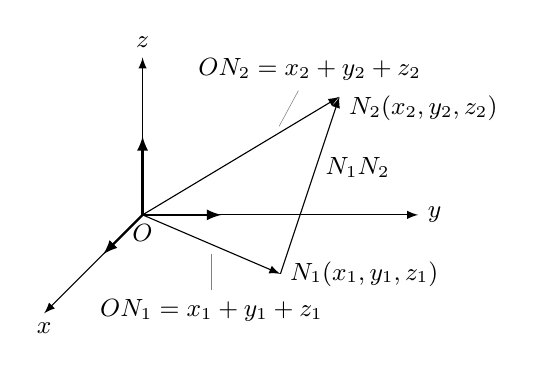
\begin{tikzpicture}[font=\small,x={(-0.5cm,-0.5cm)},y={(1cm,0)},z={(0,1cm)}]
\pgfmathsetmacro{\a}{0.5}
\pgfmathsetmacro{\b}{2}
\pgfmathsetmacro{\c}{-0.5}
\pgfmathsetmacro{\aa}{1}
\pgfmathsetmacro{\bb}{3}
\pgfmathsetmacro{\cc}{2}
\draw[-latex](0,0,0)node[below]{$O$}--(2.5,0,0)node[below]{$x$};
\draw[-latex](0,0,0)--(0,3.5,0)node[right]{$y$};
\draw[-latex](0,0,0)--(0,0,2)node[above]{$z$};
\draw[thick,-latex](0,0,0)--(1,0,0)node[pos=0.6,left,yshift=1ex]{$\ai$};
\draw[thick,-latex](0,0,0)--(0,1,0)node[above]{$\aj$};
\draw[thick,-latex](0,0,0)--(0,0,1)node[pos=0.5,left]{$\ak$};
\draw[-latex](0,0,0,)--(\a,\b,\c)node[right]{$N_1(x_1,y_1,z_1)$};
\draw(1/2*\a,1/2*\b,1/2*\c)node[pin=-90:{$\krightharpoonup{ON_1}=x_1\ai+y_1\aj+z_1\ak$}]{};
\draw[-latex](0,0,0,)--(\aa,\bb,\cc)node[right,yshift=-1ex]{$N_2(x_2,y_2,z_2)$};
\draw(2/3*\aa,2/3*\bb,2/3*\cc)node[pin={[xshift=3ex]90:{$\krightharpoonup{ON_2}=x_2\ai+y_2\aj+z_2\ak$}}]{};
\draw[-latex](\a,\b,\c)--(\aa,\bb,\cc)node[pos=0.6,right]{$\krightharpoonup{N_1N_2}$};
\end{tikzpicture}
\caption{دو نقطوں کے بیچ سمتیہ۔}
\label{شکل_سمتیہ_دو_نقطوں_کے_بیچ}
\end{minipage}
\end{figure}
\جزوحصہء{دو نقاط کے بیچ سمتیہ}
ہم نقاط \عددی{N_1(x_1,y_1,z_1)} اور \عددی{N_2(x_2,y_2,z_2)} کے بیچ سمتیہ \عددی{\krightharpoonup{N_1N_2}} کو
\begin{align*}
\krightharpoonup{N_1N_2}&=\krightharpoonup{ON_1}-\krightharpoonup{ON_2}\\
&=(x_2\ai+y_2\aj+z_2\ak)-(x_1\ai+y_1\aj+z_1\ak)\\
&=(x_2-x_1)\ai+(y_2-y_1)\aj+(z_2-z_1)\ak
\end{align*}
لکھ سکتے ہیں جو  \عددی{N_1} اور \عددی{N_2} کے محدد کی صورت میں ہے  (شکل \حوالہ{شکل_سمتیہ_دو_نقطوں_کے_بیچ})۔

یوں نقطہ \عددی{N_1(x_1,y_1,z_1)} اور \عددی{N2(x_2,y_2,z_2)} کے بیچ سمتیہ درج ذیل ہو گا۔
\begin{align}
\krightharpoonup{N_1N_2}=&=(x_2-x_1)\ai+(y_2-y_1)\aj+(z_2-z_1)\ak
\end{align}

\جزوحصہء{مقدار}
جیسا ہم جانتے ہیں، سمتیہ کی مقدار اور سمت اس کے اہم خصوصیات ہیں۔ ہم مسئلہ فیثاغورث کی مدد سے شکل \حوالہ{شکل_سمتیہ_مسئلہ_فیثاغورث_لمبائی} میں  سمتیہ \عددی{a_1\ai+a_2\aj+a_3\ak} کی مقدار (لمبائی) کا کلیہ تلاش کرتے ہیں۔ مثلث \عددی{ABC} سے
\begin{align*}
\abs{\krightharpoonup{AC}}=\sqrt{a_1^2+a_2^2}
\end{align*} 
ہو گا لہٰذا  مثلث \عددی{ACD} سے
\begin{align*}
\abs{a_1\ai+a_2\aj+a_3\ak}=\abs{\krightharpoonup{AD}}=\sqrt{\abs{\krightharpoonup{AC}}^2+\abs{\krightharpoonup{CD}}^2}=\sqrt{a_1^2+a_2^2+a_3^2}
\end{align*} 
ہو گا۔

یوں \عددی{\kvec{A}=a_1\ai+a_2\aj+a_3\ak} کی مقدار (لمبائی) درج ذیل ہو گی۔
\begin{align}\label{مساوات_سمتیہ_تین_بعدی_مقدار}
\abs{\kvec{A}}=\abs{a_1\ai+a_2\aj+a_3\ak}=\sqrt{a_1^2+a_2^2+a_3^2}
\end{align}

\begin{figure}
\centering
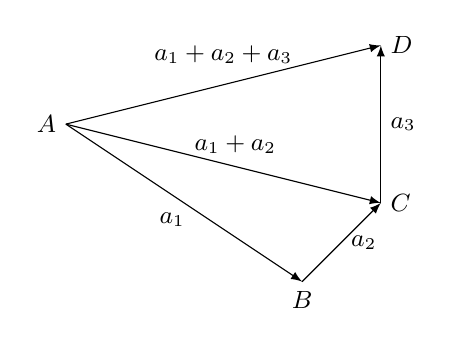
\begin{tikzpicture}[font=\small]
\draw[-latex](0,0)node[left]{$A$}--(3,-2)node[below]{$B$}node[pos=0.5,below,xshift=-1ex]{$a_1\ai$};
\draw[-latex](3,-2)--(4,-1)node[right]{$C$}node[pos=0.5,right]{$a_2\aj$};
\draw[-latex](4,-1)--(4,1)node[right]{$D$}node[pos=0.5,right]{$a_3\ak$};
\draw[-latex](0,0)--(4,-1)node[pos=0.5,above,xshift=1ex]{$a_1\ai+a_2\aj$};
\draw[-latex](0,0)--(4,1)node[pos=0.5,above,yshift=1ex]{$a_1\ai+a_2\aj+a_3\ak$};
\RightAngle{(4,-1)}{(3,-2)}{(0,0)}
\RightAngle{(4,1)}{(4,-1)}{(0,0)}
\end{tikzpicture}
\caption{قائمہ مثلث \عددی{ABC} اور \عددی{ACD} پر مسئلہ فیثاغورث کے اطلاق سے \عددی{\krightharpoonup{AD}} کی لمبائی حاصل ہوتی ہے۔}
\label{شکل_سمتیہ_مسئلہ_فیثاغورث_لمبائی}
\end{figure}
\جزوحصہء{غیر سمتی ضرب}
\ابتدا{تعریف}
اگر \عددی{c} غیر سمتی اور \عددی{\kvec{A}} ایک سمتیہ ہو تب درج ذیل ہو گا۔
\begin{align*}
c\kvec{A}=(ca_1)\ai+(ca_2)\aj+(ca_3)\ak
\end{align*}
\انتہا{تعریف}
%===============

\ابتدا{مثال}\شناخت{مثال_سمتیہ_لمبائی_سمتیہ_الف}
سمتیہ \عددی{\kvec{A}=\ai-2\aj+3\ak} کی لمبائی درج ذیل ہے۔
\begin{align*}
\abs{\kvec{A}}=\sqrt{(1)^2+(-2)^2+(3)^2}=\sqrt{1+4+9}=\sqrt{14}
\end{align*}
\انتہا{مثال}
%=====================

اگر ہم سمتیہ \عددی{\kvec{A}=a_1\ai+a_2\aj+a_3\k} کو غیر سمتی \عددی{c} سے ضرب دیں تب، مستوی میں غیر سمتی ضرب کی طرح اور انہیں وجوہات کی بنا،  \عددی{c\kvec{A}} کی لمبائی \عددی{\abs{c}} ضرب \عددی{\kvec{A}} کی لمبائی ہو گی:
\begin{gather}
\begin{aligned}
c\kvec{A}&=ca_1\ai+ca_2\aj+ca_3\ak\\
\abs{c\kvec{A}}&=\sqrt{(ca_1)^2+(ca_2)^2+(ca_3)^2}=\sqrt{c^2a_1^2+c^2a_2^2+c^2a_3^2}\\
&=\abs{c}\sqrt{a_1^2+a_2^2+a_3^2}=\abs{c}\abs{\kvec{A}}
\end{aligned}
\end{gather}

\ابتدا{مثال}
سمتیہ \عددی{\kvec{A}} مثال \حوالہ{مثال_سمتیہ_لمبائی_سمتیہ_الف} میں دیا گیا ہے۔یوں 
\begin{align*}
2\kvec{A}=2(\ai-2\aj+3\ak)=2\ai-4\aj+6\ak
\end{align*}
کی لمبائی درج ذیل ہو گی:
\begin{align*}
\sqrt{(2)^2+(-4)^2+(6)^2}&=\sqrt{4+16+36}=\sqrt{56}\\
&=\sqrt{4\cdot 14}=2\sqrt{14}=2\abs{\kvec{A}}
\end{align*}
\انتہا{مثال}
%======================

\جزوحصہء{صفر سمتیہ}
فضا میں \اصطلاح{صفر سمتیہ}\فرہنگ{سمتیہ!صفر} سے مراد سمتیہ \عددی{\kvec{0}=0\ai+0\aj+0\ak} ہے۔ مستوی میں صفر سمتیہ کی طرح فضا میں \عددی{\kvec{0}} کی لمبائی صفر ہو گی اور اس کا کوئی رخ نہیں ہو گا۔

\جزوحصہء{اکائی سمتیات}
فضا میں اکائی سمتیہ کی لمبائی \عددی{1} ہو گی۔ اساسی سمتیات درج ذیل کی بنا اکائی سمتیات ہیں۔
\begin{align*}
\abs{\ai}&=\abs{1\ai+0\aj+0\ak}=\sqrt{1^2+0^2+0^2}=1\\
\abs{\aj}&=\abs{0\ai+1\aj+0\ak}=\sqrt{0^2+1^2+0^2}=1\\
\abs{\ak}&=\abs{0\ai+0\aj+1\ak}=\sqrt{0^2+0^2+1^2}=1
\end{align*}

\جزوحصہء{مقدار اور رخ}
اگر \عددی{\kvec{A}\ne \kvec{0}} ہو تب \عددی{\tfrac{\kvec{A}}{\abs{\kvec{A}}}} ایک اکائی سمتیہ ہو گا جس کا رخ وہی ہو گا جو \عددی{\kvec{A}} کا رخ ہے۔ یوں ہم \عددی{\kvec{A}} کو اس کی مقدار ضرب رخ کی صورت میں درج ذیل لکھ سکتے ہیں۔
\begin{align}\label{مساوات_سمتیہ_فضا_لمبائی_ضرب_رخ}
\kvec{A}=\abs{\kvec{A}}\cdot\frac{\kvec{A}}{\abs{\kvec{A}}}
\end{align}

\ابتدا{مثال}
سمتیہ \عددی{\kvec{A}=\ai-2\aj+3\ak} کو اس کی مقدار ضرب رخ کی صورت میں لکھیں۔

حل:\quad
\begin{align*}
\kvec{A}&=\abs{\kvec{A}}\cdot \frac{\kvec{A}}{\abs{\kvec{A}}}&&\text{\RL{مساوات \حوالہ{مساوات_سمتیہ_فضا_لمبائی_ضرب_رخ}}}\\
&=\sqrt{14}\cdot \frac{\ai-2\aj+3\ak}{\sqrt{14}}&&\text{\RL{مثال \حوالہ{مثال_سمتیہ_لمبائی_سمتیہ_الف}}}\\
&=\sqrt{14}\big(\frac{1}{\sqrt{14}}\ai-\frac{2}{\sqrt{14}}\aj+\frac{3}{\sqrt{14}}\ak\big)=(\text{\RL{لمبائی \عددی{\kvec{A}}}})\cdot(\text{\RL{رخ \عددی{\kvec{A}}}})
\end{align*}
\انتہا{مثال}
%==============
\ابتدا{مثال}
نقطہ \عددی{N_1(1,0,1)} سے نقطہ \عددی{N_2(3,2,0)} تک سمتیہ کے رخ میں اکائی سمتیہ\عددی{\kvec{u}} تلاش کریں۔

حل:\quad
ہم \عددی{\krightharpoonup{N_1N_2}} کو اس کی لمبائی سے تقسیم کر کے \عددی{\kvec{u}} حاصل کرتے ہیں:
\begin{align*}
\krightharpoonup{N_1N_2}&=(3-1)\ai+(2-0)\aj+(0-1)\ak=2\ai+2\aj-\ak\\
\abs{\krightharpoonup{N_1N_2}}&=\sqrt{(2)^2+(2)^2+(-1)^2}=\sqrt{4+4+1}=\sqrt{9}=3\\
\kvec{u}&=\frac{\krightharpoonup{N_1N_2}}{\abs{\krightharpoonup{N_1N_2}}}=\frac{2\ai+2aj-\ak}{3}=\frac{2}{3}\ai+\frac{2}{3}\aj-\frac{1}{3}\ak
\end{align*}
\انتہا{مثال}
%===============
\ابتدا{مثال}
سمتیہ \عددی{\kvec{A}=2\ai+2\aj-\ak} کے رخ ایسا سمتیہ تلاش کریں جس کی لمبائی \عددی{6} ہو۔

حل:\quad
ہم اس سمتیہ کے رخ اکائی سمتیہ کو \عددی{6} سے ضرب کر کے جواب حاصل کرتے ہیں:
\begin{align*}
6\,\frac{\kvec{A}}{\abs{\kvec{A}}}=6\,\frac{2\ai+2\aj-\ak}{\sqrt{2^2+2^2+(-1)^2}}=6\,\frac{2\ai+2\aj-\ak}{3}=4\ai+4\aj-2\ak
\end{align*}
\انتہا{مثال}
%===========

\جزوحصہء{فضا میں فاصلہ}
فضا میں نقاط \عددی{N_1} اور \عددی{N_2} کے بیچ فاصلہ، سمتیہ \عددی{\krightharpoonup{N_1N_2}} کی  لمبائی \عددی{\abs{\krightharpoonup{N_1N_2}}} ہو گی۔

\موٹا{نقاط \عددی{N_1(x_1,y_1,z_1)} اور \عددی{N_2(x_2,y_2,z_2)} کے بیچ فاصلہ درج ذیل ہو گا۔}
\begin{align}\label{مساوات_سمتیہ_فاصلہ_فضا_میں}
\abs{\krightharpoonup{N_1N_2}}=\sqrt{(x_2-x_1)^2+(y_2-y_1)^2+(z_2-z_1)^2}
\end{align}

\ابتدا{مثال}
نقاط \عددی{N_1(2,1,5)} اور \عددی{N_2(-2,3,0)} کے بیچ فاصلہ درج ذیل ہے۔
\begin{align*}
\abs{\krightharpoonup{N_1N_2}}&=\sqrt{(-2-2)^2+(3-1)^2+(0-5)^2}\\
&=\sqrt{16+4+25}\\
&=\sqrt{45}=3\sqrt{5}
\end{align*}
\انتہا{مثال}


\جزوحصہ{کرہ}
ہم مساوات \حوالہ{مساوات_سمتیہ_فاصلہ_فضا_میں} استعمال کر کے اس کرہ کی مساوات لکھتے ہیں جس کا مرکز \عددی{N_0(x_0,y_0,z_0)} اور رداس \عددی{a} ہو۔ نقطہ \عددی{N(x,y,z)} اس صورت اس کرہ پر پایا جائے گا جب \عددی{\abs{\krightharpoonup{N_0N_1}}=a} ہو یعنی:
\begin{align*}
(x-x_0)^2+(y-y_0)^2+(z-z_0)^2=a^2
\end{align*}

\موٹا{ایک کرہ جس کا مرکز \عددی{(x_0,y_0,z_0)} اور رداس \عددی{a} ہو کی معیاری مساوات درج ذیل ہے۔}
\begin{align}\label{مساوات_سمتیہ_کرہ_معیاری}
(x-x_0)^2+(y-y_0)^2+(z-z_0)^2=a^2
\end{align}

\ابتدا{مثال}
درج ذیل کرہ کا مرکز اور رداس تلاش کریں۔
\begin{align*}
x^2+y^2+z^2+3x-4z+1=0
\end{align*}
حل:\quad
ہم مستوی میں دائرے کا مرکز اور رداس حاصل کرنے کی طرح یہاں بھی \عددی{x}، \عددی{y} اور \عددی{z} کے مربع مکمل کر کے معیاری مساوات کے ساتھ موازنہ کر کے مرکز اور رداس دریافت کرتے ہیں۔
\begin{align*}
x^2+y^2+z^2+3x-4z+1&=0\\
(x^2+3x\phantom{xx})+y^2+(z^2-4z\phantom{xx})&=-1\\
\big(x^2+3x+(\tfrac{3}{2})^2\big)+y^2+\big(z^2-4z+(-\tfrac{4}{2})^2\big)&=-1+(\tfrac{3}{2})^2+(-\tfrac{4}{2})^2\\
(x+\tfrac{3}{2})^2+y^2+(z-2)^2&=-1+\tfrac{9}{4}+4=\tfrac{21}{4}
\end{align*} 
یہ مساوات \حوالہ{مساوات_سمتیہ_کرہ_معیاری} ہے لہٰذا  \عددی{x_0=-\tfrac{3}{2}}، \عددی{y_0=0}، \عددی{z_0=2} اور \عددی{a=\tfrac{\sqrt{21}}{2}} ہیں۔ یوں مرکز \عددی{(-\tfrac{3}{2},0,2)} اور رداس \عددی{\tfrac{\sqrt{21}}{2}} ہو گا۔ 
\انتہا{مثال}
%===================
\ابتدا{مثال}\\
\begin{centering}
\renewcommand{\arraystretch}{1.5}
\begin{tabular}{lr}
مساوات اور عدم مساوات & تفصیل\\
\midrule
$x^2+y^2+z^2<4$&
کرہ \عددی{x^2+y^2+z^2=4} کا اندرون۔\\
$x^2+y^2+z^2\le4$&
\begin{minipage}{0.6\textwidth}
سطح \عددی{x^2+y^2+z^2=4}  اور اس کے اندرون پر مشتمل ٹھوس کرہ یا\\ کرہ \عددی{x^2+y^2+z^2=4} میں محدود گیند۔
\end{minipage}
 \\
$x^2+y^2+z^2>4$&
کرہ \عددی{x^2+y^2+z^2=4} کا بیرون۔\\
$x^2+y^2+z^2=4,\, z\le 0$&
کرہ \عددی{x^2+y^2+z^2=4} کا نچلا نصف حصہ۔
\end{tabular}
\end{centering}
\انتہا{مثال}
%==================
\begin{figure}
\centering
\begin{tikzpicture}
\draw[-latex](0,0)node[left]{$O$}--(2,1)node[right]{$N_2(x_2,y_2,z_2)$};
\draw[-latex](0,0)--(-0.5,2)node[left]{$N_1(x_1,y_1,z_1)$};
\draw[gray](-0.5,2)--(2,1);
\draw[-latex](0,0)--($(-0.5,2)!0.5!(2,1)$)coordinate(ka)node[above right]{$M\big(\frac{x_1+x_2}{2},\frac{y_1+y_2}{2},\frac{z_1+z_2}{2}\big)$};
\draw[-latex](-0.5,2)--(ka);
\end{tikzpicture}
\caption{نقاط \عددی{N_1} اور \عددی{N_2} کے محدد کی اوسط قطع \عددی{N_1N_2} کے وسطی نقطہ کے محدد ہوں گے۔}
\label{شکل_سمتیہ_قطع_کا_وسطی_نقطہ}
\end{figure}
\جزوحصہء{وسطی نقاط}
کسی بھی قطع کا وسطی نقطہ اوسط کی مدد سے حاصل کیا جاتا ہے۔ نقطہ \عددی{N_1(x_1,y_1,z_1)} اور \عددی{N_2(x_2,y_2,z_2)} کا وسطی نقطہ درج ذیل ہو گا۔
\begin{align*}
\big(\frac{x_1+x_2}{2},\frac{y_1+y_2}{2},\frac{z_1+z_2}{2}\big)
\end{align*}
اس کی وجہ درج ذیل ہے (شکل \حوالہ{شکل_سمتیہ_قطع_کا_وسطی_نقطہ})۔
\begin{align*}
\krightharpoonup{OM}&=\krightharpoonup{ON_1}+\frac{1}{2}\krightharpoonup{N_1N_2}=\krightharpoonup{ON_1}+\frac{1}{2}(\krightharpoonup{ON_2}-\krightharpoonup{ON_1})\\
&=\frac{1}{2}(\krightharpoonup{ON_1}+\krightharpoonup{ON_2})\\
&=\frac{x_1+x_2}{2}\ai+\frac{y_1+y_2}{2}\aj+\frac{z_1+z_2}{2}\ak
\end{align*}

\ابتدا{مثال}
نقطہ \عددی{N_1(3,-2,0)} اور \عددی{N_2(7,4,4,)} کو ملانے والی قطع کا وسطی نقطہ درج ذیل ہو گا۔
\begin{align*}
\big(\frac{3+7}{2},\frac{-2+4}{2},\frac{0+4}{2}\big)=(5,1,2)
\end{align*}
\انتہا{مثال}
%=====================

\حصہء{سوالات}
\موٹا{سلسلہ، مساوات اور عدم مساوات}\\
سوال \حوالہ{سوال_سمتیہ_جوڑی_دار_مطمئن_الف} تا سوال \حوالہ{سوال_سمتیہ_جوڑی_دار_مطمئن_ب} میں ان نقطوں کے سلسلہ کی جیومیٹریائی تفصیل بیان کریں جو دی گئی جوڑی مساوات کو مطمئن کرتے ہیں۔

\ابتدا{سوال}\شناخت{سوال_سمتیہ_جوڑی_دار_مطمئن_الف}
$x=2,\quad y=3$\\
جواب:\quad
محور \عددی{z} کے متوازی نقطہ \عددی{(2,3,0)} سے گزرتا ہوا خط۔
\انتہا{سوال}
%==================
\ابتدا{سوال}
$x=-1,\quad z=0$
\انتہا{سوال}
%==================
\ابتدا{سوال}
$y=0,\quad z=0$\\
جواب:\quad
محور \عددی{x}
\انتہا{سوال}
%==================
\ابتدا{سوال}
$x=1,\quad y=0$
\انتہا{سوال}
%==================
\ابتدا{سوال}
$x^2+y^2=4,\quad z=0$\\
جواب:\quad
مستوی \عددی{xy} میں دائرہ \عددی{x^2+y^2=4}
\انتہا{سوال}
%==================
\ابتدا{سوال}
$x^2+y^2=4,\quad z=-2$
\انتہا{سوال}
%==================
\ابتدا{سوال}
$x^2+z^2=4,\quad y=0$\\
جواب:\quad
مستوی \عددی{xz} میں دائرہ \عددی{x^2+z^2=4}
\انتہا{سوال}
%==================
\ابتدا{سوال}
$y^2+z^2=1,\quad x=0$
\انتہا{سوال}
%==================
\ابتدا{سوال}
$x^2+y^2+z^2=1,\quad x=0$\\
جواب:\quad
مستوی \عددی{yz} میں دائرہ \عددی{y^2+z^2=1}
\انتہا{سوال}
%==================
\ابتدا{سوال}
$x^2+y^2+z^2=25,\quad y=-4$
\انتہا{سوال}
%==================
\ابتدا{سوال}
$x^2+y^2+(z+3)^2=25,\quad z=0$\\
جواب:\quad
مستوی \عددی{xy} میں دائرہ \عددی{x^2+y^2=16}
\انتہا{سوال}
%==================
\ابتدا{سوال}\شناخت{سوال_سمتیہ_جوڑی_دار_مطمئن_ب}
$x^2+(y-1)^2+z^2=4,\quad y=0$
\انتہا{سوال}
%==================

سوال \حوالہ{سوال_سمتیہ_مساوات_عدم_مساوات_الف} تا سوال \حوالہ{سوال_سمتیہ_مساوات_عدم_مساوات_ب} میں ان نقاط کے سلسلہ کو جیومیٹریائی بیان کریں جو دی گئی عدم مساوات یا مساوات اور عدم مساوات کی جوڑی کو مطمئن کرتے ہیں۔   

\ابتدا{سوال}\شناخت{سوال_سمتیہ_مساوات_عدم_مساوات_الف}
(ا) 
$x\ge 0,\quad y\ge 0,\quad z=0$\quad
(ب) $x\ge 0,\quad y\le 0,\quad z=0$\\
جواب:\quad
(ا) مستوی \عددی{xy} کا ربع اول۔ (ب) مستوی \عددی{xy} کا ربع چہارم۔
\انتہا{سوال}
%=========================
\ابتدا{سوال}
\begin{enumerate}[a.]
\item
$0\le x\le 1$
\item
$0\le x\le 1,\quad 0\le y\le 1$
\item
$0\le x\le 1,\quad 0\le y\le 1,\quad 0\le z\le 1$
\end{enumerate}
\انتہا{سوال}
%=========================
\ابتدا{سوال}
\begin{enumerate}[a.]
\item
$x^2+y^2+z^2\le 1$
\item
$x^2+y^2+z^2> 1$
\end{enumerate}
جواب:\quad
(ا) رداس \عددی{1} کا گیند جس کا مرکز مبدا پر ہے۔ (ب) مبدا سے \عددی{1} اکائی سے زیادہ دور تمام نقاط۔
\انتہا{سوال} 
%=========================
\ابتدا{سوال}
(ا) 
$x^2+y^2\le 1,\, z=0$\quad
(ب)
$x^2+y^2\le 1,\, z=3$\quad
(ج) 
$x^2+y^2\le 1,\,$
جہاں \عددی{z} پر کوئی شرط لاگو نہیں ہے۔
\انتہا{سوال}
%==================
\ابتدا{سوال}
(ا)
$x^2+y^2+z^2=1,\, z\ge 0$
(ب)
$x^2+y^2+z^2\le 1,\, z\ge 0$\\
جواب:\quad
(ا) رداس \عددی{1} کا نصف بالائی کرہ جس کا مرکز مبدا پر ہے۔ (ب)  رداس \عددی{1} کا نصف بالائی ٹھوس کرہ جس کا مرکز مبدا پر ہے۔
\انتہا{سوال}
%==========
\ابتدا{سوال}\شناخت{سوال_سمتیہ_مساوات_عدم_مساوات_ب}
(ا) 
$x=y,\, z=0$
 (ب)
$x=y,\,$ 
جہاں \عددی{z} پر کوئی شور لاگو نہیں ہے۔
\انتہا{سوال}
%=====================

سوال \حوالہ{سوال_سمتیہ_جوڑی_سے_ظاہر_الف} تا سوال \حوالہ{سوال_سمتیہ_جوڑی_سے_ظاہر_ب} میں دیے گئے سلسلہ کو ایک مساوات یا جوڑی مساوات سے ظاہر کریں۔

\ابتدا{سوال}\شناخت{سوال_سمتیہ_جوڑی_سے_ظاہر_الف}
وہ مستوی جو (ا) نقطہ \عددی{(3,0,0)} پر محور \عددی{x}، (ب) نقطہ \عددی{(0,-1,0)} پر محور \عددی{y}، (ج) نقطہ \عددی{(0,0,-2)} پر محور \عددی{z} کو عمودی ہے۔\\
جواب:\quad
(ا) \عددی{x=3}، (ب) \عددی{y=-1}، (ج) \عددی{z=-2}
\انتہا{سوال}
%==================
\ابتدا{سوال}
ایک مستوی جو نقطہ \عددی{(3,-1,2)} پر (ا) محور \عددی{x}، (ب) محور \عددی{y}، (ج) محور \عددی{z} کو عمودی ہے۔ 
\انتہا{سوال}
%=============
\ابتدا{سوال}
ایک مستوی جو نقطہ \عددی{(3,-1,1)} پر (ا) مستوی \عددی{xy}، (ب) مستوی \عددی{yz}، (ج) مستوی \عددی{xz} کے متوازی ہے۔\\
جواب:\quad
(ا) \عددی{z=1}، (ب) \عددی{x=3}، (ج) \عددی{y=-1}
\انتہا{سوال}
%=============
\ابتدا{سوال}
وہ دائرہ جس کا رداس \عددی{2} اور مرکز \عددی{(0,0,0)} ہو اور جو (ا) مستوی \عددی{xy}، (ب) مستوی \عددی{yz}، (ج) مستوی \عددی{xz} میں پایا جاتا ہو۔
\انتہا{سوال}
%================
\ابتدا{سوال}
وہ دائرہ جس کا رداس \عددی{2} اور مرکز \عددی{(0,2,0)} ہو اور جو (ا) مستوی \عددی{xy}، (ب) مستوی \عددی{yz}، (ج) مستوی \عددی{y=2} میں پایا جاتا ہو۔\\
جواب:\quad
(ا) \عددی{x^2+(y-2)^2=4,\, z=0}، (ب) \عددی{(y-2)^2+z^2=4,\, x=0}،\\
 (ج) \عددی{x^2+z^2=4,\,y=2}
\انتہا{سوال}
%================
\ابتدا{سوال}
وہ دائرہ جس کا رداس \عددی{1} اور مرکز \عددی{(-3,4,1)} ہو اور جو (ا) مستوی \عددی{xy}، (ب) مستوی \عددی{yz}، (ج) مستوی \عددی{xz} کے متوازی سطح میں پایا جاتا ہو۔
\انتہا{سوال}
%================
\ابتدا{سوال}
نقطہ \عددی{(1,3,-1)} سے گزرتا خط جو (ا) محور \عددی{x}، (ب) محور \عددی{y}، (ج) محور \عددی{z} کے متوازی ہو۔\\
جواب:\quad
(ا) \عددی{y=3,\, z=-1}، (ب) \عددی{x=1,\,z=-1}، (ج) \عددی{x=1,\,y=3}
\انتہا{سوال}
%=================
\ابتدا{سوال}
فضا میں وہ نقطے معلوم کریں جن کا فاصلہ مبدا اور نقطہ \عددی{(0,2,0)} سے یکساں ہو۔  
\انتہا{سوال}
%=============
\ابتدا{سوال}
وہ دائرہ  معلوم کریں جس میں نقطہ \عددی{(1,1,3)} سے گزرتا ہوا ایسا مستوی جو محور \عددی{z} کے عمودی ہو ایک ایسے دائرہ کو جا ملتا ہو  جس کا رداس \عددی{5} اور مرکز \عددی{(0,0,0)} ہو۔\\
جواب:\quad
$x^2+y^2+z^2=25,\,z=3$
\انتہا{سوال}
%==================
\ابتدا{سوال}\شناخت{سوال_سمتیہ_جوڑی_سے_ظاہر_ب}
فضا میں ان نقطوں کا سلسلہ جن کا فاصلہ \عددی{(0,0,1)} سے \عددی{2}  اور \عددی{(0,0,-1)} سے \عددی{2} ہو۔  
\انتہا{سوال}
%==========

سوال \حوالہ{سوال_سمتیہ_عدم_مساوات_پیش_الف} تا سوال \حوالہ{سوال_سمتیہ_عدم_مساوات_پیش_ب} میں دیے سلسلہ کی عدم مساوات پیش کریں۔

\ابتدا{سوال}\شناخت{سوال_سمتیہ_عدم_مساوات_پیش_الف}
سطح \عددی{z=0} اور \عددی{z=1} کے بیچ پٹی بشمول ان سطحوں کے۔\\
جواب:\quad
$0\le z\le 1$
\انتہا{سوال}
%=====================
\ابتدا{سوال}
پہلے ثمن میں محددی سطحوں اور سطحوں \عددی{x=2}، \عددی{y=2} اور \عددی{z=2} میں محدود ٹھوس مکعب۔
\انتہا{سوال}
%===============
\ابتدا{سوال}
نصف فضا جو مستوی \عددی{xy} اور اس کے نیچے  نقطوں پر مشتمل ہے۔ \\
جواب:\quad
$z\le 0$
\انتہا{سوال}
%==================
\ابتدا{سوال}
رداس \عددی{1} کا کرہ جس کا مرکز مبدا پر ہو کا بالائی نصف حصہ۔
\انتہا{سوال}
%====================
\ابتدا{سوال}
رداس \عددی{1} کا کرہ جس کا مرکز \عددی{(1,1,1)} ہو کا (ا) اندرون، (ب) بیرون۔\\
جواب:\quad
(ا) \عددی{(x-1)^2+(y-1)^2+(z-1)^2<1}، \\
(ب) \عددی{(x-1)^2+(y-1)^2+(z-1)^2>1}
\انتہا{سوال}
%=====================
\ابتدا{سوال}\شناخت{سوال_سمتیہ_عدم_مساوات_پیش_ب}
رداس \عددی{1} اور \عددی{2} کے کرہ جن کے مراکز مبدا پر ہوں میں بند خطہ۔ (بند خطہ سے مراد ہے کہ کرہ کی سطحیں بھی اس خطہ میں شامل ہوں گی۔ کروی سطحوں کو شامل نہ کرنے کے لئے ہم آزاد خطے کی اصطلاح استعمال کرتے ہیں۔)
\انتہا{سوال}
%======================

\موٹا{لمبائی اور رخ}\\
سوال \حوالہ{سوال_سمتیہ_لمبائی_رخ_صورت_الف} تا سوال \حوالہ{سوال_سمتیہ_لمبائی_رخ_صورت_ب} میں دیے سمتیہ کو اس کی لمبائی ضرب رخ کی صورت میں لکھیں۔

\ابتدا{سوال}\شناخت{سوال_سمتیہ_لمبائی_رخ_صورت_الف}
$2\ai+\aj-2\ak$\\
جواب:\quad
$3(\tfrac{2}{3}\ai+\tfrac{1}{3}\aj-\tfrac{2}{3}\ak)$
\انتہا{سوال}
%=====================
\ابتدا{سوال}
$3\ai-6\aj+2\ak$
\انتہا{سوال}
%=========================
\ابتدا{سوال}
$\ai+4\aj-8\ak$\\
جواب:\quad
$9(\tfrac{1}{9}\ai+\tfrac{4}{9}\aj-\tfrac{8}{9}\ak)$
\انتہا{سوال}
%=========================
\ابتدا{سوال}
$9\ai-2\aj+6\ak$
\انتہا{سوال}
%=========================
\ابتدا{سوال}
$5\ak$\\
جواب:\quad
$5(\ak)$
\انتہا{سوال}
%=========================
\ابتدا{سوال}
$-4\aj$
\انتہا{سوال}
%=========================
\ابتدا{سوال}
$\tfrac{3}{5}\ai+\tfrac{4}{5}\ak$\\
جواب:\quad
$1(\tfrac{3}{5}\ai+\tfrac{4}{5}\ak)$
\انتہا{سوال}
%=========================
\ابتدا{سوال}
$\tfrac{1}{\sqrt{2}}\ai-\tfrac{1}{\sqrt{2}}\ak$
\انتہا{سوال}
%=========================
\ابتدا{سوال}
$\tfrac{1}{\sqrt{6}}\ai-\tfrac{1}{\sqrt{6}}\ai-\tfrac{1}{\sqrt{6}}\ak$\\
جواب:\quad
$\sqrt{\tfrac{1}{2}}(\tfrac{1}{\sqrt{3}}\ai-\tfrac{1}{\sqrt{3}}\aj-\tfrac{1}{\sqrt{3}}\ak)$
\انتہا{سوال}
%=========================
\ابتدا{سوال}\شناخت{سوال_سمتیہ_لمبائی_رخ_صورت_ب}
$\tfrac{\ai}{\sqrt{3}}+\tfrac{\aj}{\sqrt{3}}+\tfrac{\ak}{\sqrt{3}}$
\انتہا{سوال}
%=========================

\ابتدا{سوال}
سمتیات کی لمبائیاں اور رخ دیے گئے ہیں۔ ان سمتیات کو تلاش کریں۔ کوشش کریں کہ حساب زبانی کریں۔\\
\begin{center}
\renewcommand{\arraystretch}{1.5}
\begin{tabular}{rLL}
\text{شمار}&\text{لمبائی}&\text{رخ}\\
\midrule
(ا)&
2&\ai\\
(ب)&
\sqrt{3}&-\ak\\
(ج)&
\tfrac{1}{2}&\tfrac{3}{5}\aj+\tfrac{4}{5}\ak\\
(د)&
7&\tfrac{6}{7}\ai-\tfrac{2}{7}\aj+\tfrac{3}{7}\ak
\end{tabular}
\end{center}
جواب:\quad
(ا) \عددی{2\ai}، (ب) \عددی{-\sqrt{3}\ak}، (ج) \عددی{\tfrac{3}{10}\aj+\tfrac{2}{5}\ak}، (د) \عددی{6\ai-2\aj+3\ak} 
\انتہا{سوال}
%======================
\ابتدا{سوال}
سمتیات کی لمبائیاں اور رخ دیے گئے ہیں۔ ان سمتیات کو تلاش کریں۔ کوشش کریں کہ حساب زبانی کریں۔\\
\begin{center}
\renewcommand{\arraystretch}{1.5}
\begin{tabular}{rLL}
\text{شمار}&\text{لمبائی}&\text{رخ}\\
\midrule
(ا)&
7&-\aj\\
(ب)&
\sqrt{2}&-\tfrac{3}{5}\ai-\tfrac{4}{5}\ak\\
(ج)&
\tfrac{13}{12}&\tfrac{3}{13}\ai-\tfrac{4}{13}\aj-\tfrac{12}{13}\ak\\
(د)&
a>0&\tfrac{1}{\sqrt{2}}\ai+\tfrac{1}{\sqrt{3}}\aj-\tfrac{1}{\sqrt{6}}\ak
\end{tabular}
\end{center}
\انتہا{سوال}
%======================
\ابتدا{سوال}
سمتیہ \عددی{\kvec{A}=12\ai-5\ak} کے رخ ایسا سمتیہ تلاش کریں جس کی لمبائی \عددی{7} ہو۔\\
جواب:\quad
$\tfrac{7}{13}(12\ai-5\ak)$
\انتہا{سوال}
%=================
\ابتدا{سوال}
سمتیہ \عددی{\kvec{A}=\ai+\aj+\ak} کے رخ ایسا سمتیہ تلاش کریں جس کی لمبائی \عددی{\sqrt{5}} ہو۔
\انتہا{سوال}
%=================
\ابتدا{سوال}
سمتیہ \عددی{\kvec{A}=2\ai-3\aj+6\ak} کے مخالف رخ ایسا سمتیہ تلاش کریں جس کی لمبائی \عددی{5} ہو۔\\
جواب:\quad
$-\tfrac{10}{7}\ai+\tfrac{15}{7}\aj-\tfrac{30}{7}\ak$
\انتہا{سوال}
%=================
\ابتدا{سوال}
سمتیہ \عددی{\kvec{A}=\tfrac{1}{2}\ai-\tfrac{1}{2}\aj-\tfrac{1}{2}\ak} کے مخالف رخ ایسا سمتیہ تلاش کریں جس کی لمبائی \عددی{3} ہو۔
\انتہا{سوال}
%=================

\موٹا{سمتیات کا تعین بذریعہ نقاط، وسطی نقاط اور فاصلہ}

سوال \حوالہ{سوال_سمتیہ_معلوم_کریں_الف} تا سوال \حوالہ{سوال_سمتیہ_معلوم_کریں_ب} میں درج ذیل معلوم کریں۔
\begin{enumerate}[a.]
\item
نقاط \عددی{N_1} اور \عددی{N_2} کے بیچ فاصلہ،
\item
رخ \عددی{\krightharpoonup{N_1N_2}}،
\item
قطع \عددی{N_1N_2} کا وسطی نقطہ۔
\end{enumerate}

\ابتدا{سوال}\شناخت{سوال_سمتیہ_معلوم_کریں_الف}
$N_1(1,1,1),\quad N_2(3,3,0)$\\
جواب:\quad
(ا) \عددی{3}، (ب) \عددی{\tfrac{2}{3}\ai+\tfrac{2}{3}\aj-\tfrac{1}{3}\ak}، (ج) \عددی{(2,2,\tfrac{1}{2})}
\انتہا{سوال}
%======================
\ابتدا{سوال}
$N_1(-1,1,5),\quad N_2(2,5,0)$
\انتہا{سوال}
%======================
\ابتدا{سوال}
$N_1(1,4,5),\quad N_2(4,-2,7)$\\
جواب:\quad
(ا) \عددی{7}، (ب) \عددی{\tfrac{3}{7}\ai-\tfrac{6}{7}\aj+\tfrac{2}{7}\ak}، (ج) \عددی{(\tfrac{5}{2},1,6)}
\انتہا{سوال}
%======================
\ابتدا{سوال}
$N_1(3,4,5),\quad N_2(2,3,4)$
\انتہا{سوال}
%======================
\ابتدا{سوال}
$N_1(0,0,0),\quad N_2(2,-2,-2)$\\
جواب:\quad
(ا) \عددی{2\sqrt{3}}، (ب) \عددی{\tfrac{1}{\sqrt{3}}\ai-\tfrac{1}{\sqrt{3}}\aj-\tfrac{1}{\sqrt{3}}\ak}، (ج) \عددی{(1,-1,-1)}
\انتہا{سوال}
%======================
\ابتدا{سوال}\شناخت{سوال_سمتیہ_معلوم_کریں_ب}
$N_1(5,3,-2),\quad N_2(0,0,0)$
\انتہا{سوال}
%======================

\ابتدا{سوال}
اگر \عددی{\krightharpoonup{AB}=\ai+4\aj-2\ak} اور \عددی{B} نقطہ \عددی{(5,1,3)} ہو تب نقطہ \عددی{A} تلاش کریں۔\\
جواب:\quad
$A(4,-3,5)$
\انتہا{سوال}
%===========
\ابتدا{سوال}
اگر \عددی{\krightharpoonup{AB}=-7\ai+3\aj+8\ak} اور \عددی{A} نقطہ \عددی{(-2,-3,6)} ہو تب نقطہ \عددی{B} تلاش کریں۔
\انتہا{سوال}
%===========

\موٹا{کرہ}\\
سوال \حوالہ{سوال_سمتیہ_رداس_مرکز_الف} تا سوال \حوالہ{سوال_سمتیہ_رداس_مرکز_ب} میں کرہ کے رداس اور مراکز تلاش کریں۔

\ابتدا{سوال}\شناخت{سوال_سمتیہ_رداس_مرکز_الف}
$(x+2)^2+y^2+(z-2)^2=8$\\
جواب:\quad
$C(-2,0,2),\quad a=2\sqrt{2}$
\انتہا{سوال}
%====================
\ابتدا{سوال}
$(x+\tfrac{1}{2})^2+(y+\tfrac{1}{2})^2+(z+\tfrac{1}{2})^2=\tfrac{21}{4}$
\انتہا{سوال}
%====================
\ابتدا{سوال}
$(x-\sqrt{2})^2+(y-\sqrt{2})^2+(z+\sqrt{2})^2=2$\\
جواب:\quad
$C(\sqrt{2},\sqrt{2},-\sqrt{2}),\quad a=\sqrt{2}$
\انتہا{سوال}
%====================
\ابتدا{سوال}\شناخت{سوال_سمتیہ_رداس_مرکز_ب}
$x^2+(y+\tfrac{1}{3})^2+(z-\tfrac{1}{3})^2=\tfrac{29}{9}$
\انتہا{سوال}
%====================

سوال \حوالہ{سوال_سمتیہ_کرہ_رداس_مرکز_سے_معلوم_الف} تا سوال \حوالہ{سوال_سمتیہ_کرہ_رداس_مرکز_سے_معلوم_ب} میں کرہ کے رداس اور مراکز دیے گئے ہیں۔ ان کرہ کی مساوات حاصل کریں۔

\ابتدا{سوال}\شناخت{سوال_سمتیہ_کرہ_رداس_مرکز_سے_معلوم_الف}
رداس \عددی{\sqrt{14}}، مرکز \عددی{(1,2,3)}\\
جواب:\quad
$(x-1)^2+(y-2)^2+(z-3)^2=14$
\انتہا{سوال}
%======================
\ابتدا{سوال}
رداس \عددی{2}، مرکز \عددی{(0,-1,5)}
\انتہا{سوال}
%======================
\ابتدا{سوال}
رداس \عددی{\sqrt{3}}، مرکز \عددی{(-2,0,0)}\\
جواب:\quad
$(x+2)^2+y^2+z^2=3$
\انتہا{سوال}
%======================
\ابتدا{سوال}\شناخت{سوال_سمتیہ_کرہ_رداس_مرکز_سے_معلوم_ب}
رداس \عددی{7}، مرکز \عددی{(0,-7,0)}
\انتہا{سوال}
%======================

سوال \حوالہ{سوال_سمتیہ_کرہ_رداس_تلاش_الف} تا سوال \حوالہ{سوال_سمتیہ_کرہ_رداس_تلاش_ب} میں دیے کرہ کے رداس اور مراکز دریافت کریں۔

\ابتدا{سوال}\شناخت{سوال_سمتیہ_کرہ_رداس_تلاش_الف}
$x^2+y^2+z^2+4x-4z=0$\\
جواب:\quad
$C(-2,0,2),\quad a=\sqrt{8}$
\انتہا{سوال}
%=========================
\ابتدا{سوال}
$x^2+y^2+z^2-6y+8z=0$
\انتہا{سوال}
%=========================
\ابتدا{سوال}
$2x^2+2y^2+2z^2+x+y+z=9$\\
جواب:\quad
$C(-\tfrac{1}{4},-\tfrac{1}{4},-\tfrac{1}{4}),\quad a=\tfrac{5\sqrt{3}}{4}$
\انتہا{سوال}
%=========================
\ابتدا{سوال}\شناخت{سوال_سمتیہ_کرہ_رداس_تلاش_ب}
$3x^2+3y^2+3z^2+2y-2z=9$
\انتہا{سوال}
%=========================

\ابتدا{سوال}
نقطہ \عددی{N(x,y,z)} سے (ا) محور \عددی{x}، (ب) محور \عددی{y}، (ج) محور \عددی{z} تک فاصلہ تلاش کریں۔\\
جواب:\quad
(ا) \عددی{\sqrt{y^2+z^2}}، (ب) \عددی{\sqrt{x^2+z^2}}، (ج) \عددی{\sqrt{x^2+y^2}}
\انتہا{سوال}
%==========================
\ابتدا{سوال}
نقطہ \عددی{N(x,y,z)} سے (ا) سطح \عددی{xy}، (ب) سطح \عددی{yz}، (ج) سطح \عددی{xz} تک فاصلہ تلاش کریں۔
\انتہا{سوال}
%==========================

\موٹا{سمتیات اور جیومیٹری}\\
\ابتدا{سوال}
نقاط \عددی{A(4,2,0)}، \عددی{B(1,3,0)} اور \عددی{C(1,1,3)}  یکساں کثافت کے باریک مثلث کے راس ہیں۔ 
\begin{enumerate}[a.]
\item
نقطہ \عددی{C} سے \عددی{AB} کے وسطی نقطہ \عددی{M} تک سمتیہ تلاش کریں۔
\item
نقطہ \عددی{C} سے وسطانیہ \عددی{CM} پر \عددی{C} سے \عددی{\tfrac{2}{3}} فاصلہ تک سمتیہ تلاش کریں۔
\item
مثلث \عددی{ABC} کے وسطانیوں کے نقطہ تقاطع کے محدد تلاش کریں۔
\end{enumerate}
جواب:\quad
(ا) \عددی{\tfrac{3}{2}\ai+\tfrac{3}{2}\aj-3\ak}، (ب) \عددی{\ai+\aj-2\ak}، (ج) \عددی{(2,2,1)}
\انتہا{سوال}
%=======================
\ابتدا{سوال}
ایک مثلث جس کے راس \عددی{A(1,-1,2)}، \عددی{B(2,1,3)} اور \عددی{C(-1,2,-1)} ہیں کے وسطانیوں کے نقطہ تقاطع تک مبدا سے سمتیہ تلاش کریں۔ 
\انتہا{سوال}
%===================
\ابتدا{سوال}
فضا میں چار الاضلاع کے راس \عددی{A}، \عددی{B}، \عددی{C} اور \عددی{D} ہیں۔ یہ چار الاضلاع ضروری نہیں کہ مستوی ہو۔ دکھائیں کہ مخالف اضلاع کے وسطانی نقطوں کو جوڑنے والے قطعات ایک دوسرے کو نصف میں قطع کرتے ہیں۔ (اشارہ: دکھائیں کہ ان قطعات کے وسطی نقاط یکساں ہیں۔)
\انتہا{سوال}
%=====================
\ابتدا{سوال}
منظم \عددی{n} کثیر الاضلاع کے مرکز سے اس کے راس تک سمتیات بنائے جاتے ہیں۔ دکھائیں کہ ان سمتیات کا مجموعہ صفر ہو گا۔ (اشارہ: کثیر الاضلاع کو اپنے مرکز کے گرد گھمانے سے اس مجموعہ پر کیا اثر ہو گا؟)
\انتہا{سوال}
%=================
\ابتدا{سوال}
فرض کریں ایک مثلث کے راس \عددی{A}، \عددی{B} اور \عددی{C} ہیں جبکہ مطابقتی مخالف اضلاع کے وسطی نقاط \عددی{a}، \عددی{b} اور \عددی{c} ہیں۔ دکھائیں کہ \عددی{\krightharpoonup{Aa}+\krightharpoonup{Bb}+\krightharpoonup{Cc}=0} ہو گا۔
\انتہا{سوال}
%==================

\حصہ{ضرب نقطہ}
ہم اب ضرب نقطہ پر غور کرتے ہیں جو سمتیات کو آپس میں ضرب دینے کے دو طریقوں میں سے ایک ہے۔ چونکہ ضرب نقطہ کا نتیجہ غیر سمتی ہوتا ہے لہٰذا ضرب نقطہ کو \اصطلاح{غیر سمتی ضرب}\فرہنگ{غیر سمتی!ضرب}\فرہنگ{ضرب!غیر سمتی}\حاشیہب{scalar product}\فرہنگ{scalar!product} بھی کہتے ہیں۔

\جزوحصہء{ضرب نقطہ}
جب دو غیر صفر سمتیات \عددی{\kvec{A}} اور \عددی{\kvec{B}} کے ابتدائی نقاط  کو ایک ہی نقطہ پر رکھا جائے تب ان سمتیات کے بیچ زاویہ \عددی{0\le \theta\le \pi} پایا جاتا ہے۔ یہ زاویہ \عددی{\kvec{A}} اور \عددی{\kvec{B}} کے بیچ زاویہ کہلاتا ہے۔
\begin{figure}
\centering
\begin{minipage}{0.45\textwidth}
\centering
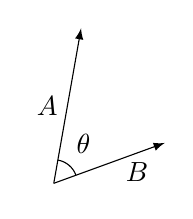
\begin{tikzpicture}
\draw[-latex](0,0)--(20:1.5)node[pos=0.75,below]{$\kvec{B}$};
\draw[-latex](0,0)--(80:2)node[pos=0.5,left]{$\kvec{A}$};
\draw([shift={(20:0.3)}]0,0) arc (20:80:0.3)node[pos=0.6,above right]{$\theta$};
\end{tikzpicture}
\caption{سمتیات \عددی{\kvec{A}} اور \عددی{\kvec{B}} کے بیچ زاویہ۔}
\label{شکل_سمتیہ_سمتیات_کے_بیچ_زاویہ}
\end{minipage}\hfill
\begin{minipage}{0.45\textwidth}
\centering
\begin{tikzpicture}[font=\small,y={(0,0.6cm)}]
\draw[-latex](0,0)--(-1,-1)node[left]{$x$};
\draw[-latex](0,0)--(1,0)node[right]{$y$};
\draw[-latex](0,0)--(0,3.5)node[left]{$z$};
\draw[thick,-latex](0,0)--(0,3)node[pos=0.8,right]{\kvec{A}=$3\ak$};
\draw[thick,-latex](0,0)--(-{1/sqrt(2)},{1/sqrt(2)})node[pos=0.6,below]{$2$}node[left]{\kvec{B}=$\sqrt{2}\ai+\sqrt{2}\ak$}coordinate(kt);
\draw[dashed](kt)--(-{1/sqrt(2)},{-1/sqrt(2)})node[right]{$\sqrt{2}$};
\draw[dashed](kt)--(0,{2*1/sqrt(2)})node[right]{$\sqrt{2}$};
\draw([shift={(90:0.3)}]0,0) arc (90:135:0.3)node[pos=0.7,above]{$\tfrac{\pi}{4}$};
\end{tikzpicture}
\caption{سمتیات برائے مثال \حوالہ{مثال_سمتیہ_ضرب_نقطہ}}
\label{شکل_مثال_سمتیہ_ضرب_نقطہ}
\end{minipage}
\end{figure}

\ابتدا{تعریف}
سمتیات \عددی{\kvec{A}} اور \عددی{\kvec{B}} کے غیر سمتی ضرب (ضرب نقطہ) سے مراد درج ذیل عدد ہے
\begin{align}\label{مساوات_سمتیہ_غیر_سمتی_ضرب_تعریف}
\kvec{A}\cdot\kvec{B}=\abs{\kvec{A}}\abs{\kvec{B}}\cos\theta
\end{align}
جہاں \عددی{\theta} سمتیات \عددی{\kvec{A}} اور \عددی{\kvec{B}} کے بیچ زاویہ  ہے (شکل \حوالہ{شکل_سمتیہ_سمتیات_کے_بیچ_زاویہ})۔
\انتہا{تعریف}
%===========================  

الفاظ میں،  \عددی{\kvec{A}\cdot\kvec{B}} سے مراد \عددی{\kvec{A}} کی لمبائی ضرب \عددی{\kvec{B}} کی لمبائی ضرب اس زاویہ کا کوسائن جو ان سمتیات کے بیچ پایا جاتا ہے۔

سمتیات \عددی{\kvec{A}} اور \عددی{\kvec{B}} کے ضرب نقطہ کو \عددی{\kvec{A}} اور \عددی{\kvec{B}} کے بیچ نقطہ سے ظاہر کیا جاتا ہے یعنی \عددی{\kvec{A}\cdot\kvec{B}} جس کی بنا یہ ضرب نقطہ کہلاتا ہے۔

\ابتدا{مثال}\شناخت{مثال_سمتیہ_ضرب_نقطہ}
سمتیات \عددی{\kvec{A}=3\ak} اور \عددی{\kvec{B}=\sqrt{2}\ai+\sqrt{2}\ak} کے ضرب نقطہ درج ذیل ہو گا (شکل \حوالہ{شکل_مثال_سمتیہ_ضرب_نقطہ})۔
\begin{align*}
\kvec{A}\cdot\kvec{A}=\abs{\kvec{A}}\abs{\kvec{B}}\cos\theta=(3)(2)\cos\frac{\pi}{4}=6\cdot\frac{\sqrt{2}}{2}=3\sqrt{2}
\end{align*}
\انتہا{مثال}
%=======================

چونکہ غیر سمتی ضرب کی علامت \عددی{\cos\theta} پر منحصر ہے لہٰذا غیر سمتی ضرب کا نتیجہ زاویہ حادہ کی صورت میں مثبت، زاویہ منفرجہ کی صورت میں  منفی (اور زاویہ قائمہ کی صورت میں صفر ہو گا)۔

چونکہ سمتیہ \عددی{\kvec{A}} کا اپنے ساتھ زاویہ صفر ہے  اور \عددی{\cos 0=1} ہوتا ہے لہٰذا
\begin{align*}
\kvec{A}\cdot \kvec{A}=\abs{\kvec{A}}\abs{\kvec{A}}\cos 0=\abs{\kvec{A}}\abs{\kvec{A}}(1)=\abs{\kvec{A}}^2
\end{align*}
یعنی
\begin{align}
\abs{\kvec{A}}=\sqrt{\kvec{A}\cdot \kvec{A}}
\end{align}
ہو گا۔

\جزوحصہ{حساب}
کارتیسی نظام میں \عددی{\kvec{A}\cdot\kvec{B}} کا حساب \عددی{\kvec{A}} اور \عددی{\kvec{B}} کے اجزاء سے حاصل کرنے کی خاطر ہم درج ذیل لیتے ہیں۔
\begin{align*}
\kvec{A}&=a_1\ai+a_2\aj+a_3\ak,\\
\kvec{B}&=b_1\ai+b_2\aj+b_3\ak,\\
\kvec{C}&=\kvec{B}-\kvec{A}=(b_1-a_1)\ai+(b_2-a_2)\aj+(b_3-a_3)\ak
\end{align*}

ایک مثلث جس کے اضلاع \عددی{\kvec{A}}، \عددی{\kvec{B}} اور \عددی{\kvec{C}} ہوں کے لئے قاعدہ کوسائن درج ذیل ہو گا (شکل \حوالہ{شکل_سمتیہ_قاعدہ_کوسائن})۔
\begin{align*}
\abs{\kvec{C}}^2&=\abs{\kvec{A}}^2+\abs{\kvec{B}}^2-2\abs{\kvec{A}}\abs{\kvec{B}}\cos\theta\\
\abs{\kvec{A}}\abs{\kvec{B}}\cos\theta&=\frac{\abs{\kvec{A}}^2+\abs{\kvec{B}}^2-\abs{\kvec{C}}^2}{2}
\end{align*} 

اس مساوات کا بایاں ہاتھ \عددی{\kvec{A}\cdot\kvec{B}} ہے۔ ہم \عددی{\kvec{A}}، \عددی{\kvec{B}} اور \عددی{\kvec{C}} کے اجزاء کا مربع لے کر مساوات کے دائیں ہاتھ کی قیمت حاصل کرتے ہیں (مساوات \حوالہ{مساوات_سمتیہ_تین_بعدی_مقدار})۔ یوں
\begin{align}\label{مساوات_سمتیہ_غیر_سمتی_ضرب_کا_کلیہ}
\kvec{A}\cdot\kvec{B}=a_1b_1+a_2b_2+a_3b_3
\end{align}
حاصل ہوتا ہے لہٰذا دو سمتیات کا غیر سمتی ضرب لینے کی خاطر ہم اس کے مطابقتی \عددی{\ai}، \عددی{\aj} اور \عددی{a\k} اجزاء کو ضرب دے کر ان کا مجموعہ لیتے ہیں۔
\begin{figure}
\centering
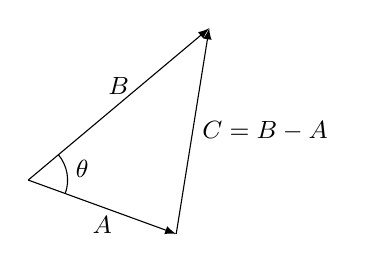
\begin{tikzpicture}[font=\small,]
\draw[-latex](0,0)--(-20:2)coordinate(a)node[pos=0.5,below]{$\kvec{A}$};
\draw[-latex](0,0)--(40:3)coordinate(b)node[pos=0.5,above]{$\kvec{B}$};
\draw[-latex](a)--(b)node[pos=0.5,right]{$\kvec{C}=\kvec{B}-\kvec{A}$};
\draw([shift={(-20:0.5)}]0,0) arc (-20:40:0.5)node[pos=0.6,right]{$\theta$};
\end{tikzpicture}
\caption{ایک مثلث جس کے اضلاع \عددی{\kvec{A}}، \عددی{\kvec{B}} اور \عددی{\kvec{C}=\kvec{B}-\kvec{A}} ہوں پر قاعدہ کوسائن کے اطلاق سے مساوات \حوالہ{مساوات_سمتیہ_غیر_سمتی_ضرب_کا_کلیہ} حاصل ہو گا۔}
\label{شکل_سمتیہ_قاعدہ_کوسائن}
\end{figure}

مساوات \حوالہ{مساوات_سمتیہ_غیر_سمتی_ضرب_تعریف} کو \عددی{\theta} کے لئے حل کر کے ان سمتیات کے بیچ زاویہ حاصل ہو گا۔
\begin{align}\label{مساوات_سمتیہ_بیچ_زاویہ}
\theta&=\cos^{-1}\big(\frac{\kvec{A}\cdot\kvec{B}}{\abs{\kvec{A}}\abs{\kvec{B}}}\big)&&\text{\RL{سمتیات کے بیچ زاویہ}}
\end{align}

چونکہ  الٹ کوسائن کی قیمت \عددی{[0,\pi]} میں پائی جاتی ہے  لہٰذا مساوات \حوالہ{مساوات_سمتیہ_بیچ_زاویہ} خود بخود \عددی{\kvec{A}} اور \عددی{\kvec{B}} کے بیچ زاویہ دیتی ہے۔

\ابتدا{مثال}
سمتیات\عددی{\kvec{A}=\ai-2\aj-2\ak} اور \عددی{\kvec{B}=6\ai+3\aj+2\ak} کے بیچ زاویہ تلاش کریں۔

حل:\quad
ہم مساوات \حوالہ{مساوات_سمتیہ_بیچ_زاویہ} استعمال کرتے ہیں۔
\begin{align*}
\kvec{A}\cdot\kvec{B}&=(1)(6)+(-2)(3)+(-2)(2)=6-6-4=-4\\
\abs{\kvec{A}}&=\sqrt{(1)^2+(-2)^2+(-2)^2}=\sqrt{9}=3\\
\abs{\kvec{B}}&=\sqrt{(6)^2+(3)^2+(2)^2}=\sqrt{49}=7\\
\theta&=\cos^{-1}\big(\frac{\kvec{A}\cdot\kvec{B}}{\abs{\kvec{A}}\abs{\kvec{B}}}\big)\\
&=\cos^{-1}\big(\frac{-4}{(3)(7)}\big)=\cos^{-1}\big(-\frac{4}{21}\big)\approx 1.76 \, \text{ریڈیئن}
\end{align*}
\انتہا{مثال}
%====================

\جزوحصہء{قواعد ضرب نقطہ}
ہم ضرب نقطہ کی مساوات \عددی{\kvec{A}\cdot\kvec{B}=a_1b_1+a_2b_2+c_1c_2} سے  درج ذیل لکھ سکتے ہیں۔
\begin{align}\label{مساوات_سمتیہ_قواعد_ضرب_نقطہ_الف}
\kvec{A}\cdot\kvec{B}=\kvec{B}\cdot\kvec{A}
\end{align}
دوسرے لفظوں میں، ضرب نقطہ \اصطلاح{قابل تبادل}\فرہنگ{قابل تبادل}\حاشیہب{commutative}\فرہنگ{commutative} ہے۔ ہم مساوات \حوالہ{مساوات_سمتیہ_غیر_سمتی_ضرب_کا_کلیہ} سے  یہ بھی دیکھتے ہیں کہ مستقل (یا غیر سمتی) عدد \عددی{c} کی صورت میں درج ذیل ہو گا۔
\begin{align}\label{مساوات_سمتیہ_قواعد_ضرب_نقطہ_ب}
(c\kvec{A})\cdot\kvec{B}=\kvec{A}\cdot(c\kvec{B})=c(\kvec{A}\cdot\kvec{B})
\end{align}
اگر \عددی{\kvec{C}=c_1\ai+c_2\aj+c_3\ak} کوئی تیسرا سمتیہ ہو تب درج ذیل لکھا جا سکتا ہے۔
\begin{align*}
\kvec{A}\cdot(\kvec{B}+\kvec{C})&=a_1(b_1+c_1)+a_2(b_2+c_2)+a_3(b_3+c_3)\\
&=(a_1b_1+a_2b_2+a_3b_3)+(a_1c_1+a_2c_2+a_3c_3)\\
&=\kvec{A}\cdot\kvec{B}+\kvec{A}\cdot\kvec{C}
\end{align*}
اس طرح ضرب نقطہ قانون تقسیم (درج ذیل)  کو مطمئن کرتا ہے۔
\begin{align}\label{مساوات_سمتیہ_قواعد_ضرب_نقطہ_پ}
\kvec{A}\cdot(\kvec{B}+\kvec{C})=\kvec{A}\cdot\kvec{B}+\kvec{A}\cdot\kvec{C}
\end{align}
اس کو مساوات \حوالہ{مساوات_سمتیہ_قواعد_ضرب_نقطہ_الف} کے ساتھ ملا کر درج ذیل لکھا جا سکتا ہے۔
\begin{align}\label{مساوات_سمتیہ_قواعد_ضرب_نقطہ_ت}
(\kvec{A}+\kvec{B})\cdot\kvec{C}=\kvec{A}\cdot\kvec{C}+\kvec{B}\cdot\kvec{C}
\end{align}
مساوات \حوالہ{مساوات_سمتیہ_قواعد_ضرب_نقطہ_پ} اور مساوات \حوالہ{مساوات_سمتیہ_قواعد_ضرب_نقطہ_ت} ہمیں سمتیات کے مجموعوں کو، الجبرا کے قواعد کے مطابق، آپس میں ضرب دینے کی اجازت دیتے ہیں۔ مثال کے طور پر:
\begin{align}\label{مساوات_سمتیہ_قواعد_ضرب_نقطہ_ٹ}
(\kvec{A}+\kvec{B})\cdot(\kvec{C}+\kvec{D})=\kvec{A}\cdot\kvec{C}+\kvec{A}\cdot\kvec{D}+\kvec{B}\cdot\kvec{C}+\kvec{B}\cdot\kvec{D}
\end{align}

\جزوحصہء{عمودی سمتیات}
دو غیر صفر سمتیات \عددی{\kvec{A}} اور \عددی{\kvec{B}} تب \اصطلاح{عمودی}\فرہنگ{عمودی}\حاشیہب{orthogonal}\فرہنگ{orthogonal} ہوں گے جب ان  کے بیچ زاویہ \عددی{\tfrac{\pi}{2}} ہو ۔ یوں \عددی{\cos\tfrac{\pi}{2}=0} کی بنا عمودی سمتیات کے لئے \عددی{\kvec{A}\cdot\kvec{B}=0} ہو گا۔ اسی طرح  اگر \عددی{\kvec{A}} اور \عددی{\kvec{B}} غیر صفر سمتیات ہوں اور \عددی{\kvec{A}\cdot\kvec{B}=\abs{\kvec{A}}\abs{\kvec{B}}\cos\theta=0} ہو تب \عددی{\cos\theta=0} یعنی \عددی{\theta=\cos^{-1}0=\tfrac{\pi}{2}} ہو گا۔

دو غیر صفر سمتیات \عددی{\kvec{A}} اور \عددی{\kvec{B}} صرف اور صرف اس صورت عمودی ہوں گے جب \عددی{\kvec{A}\cdot\kvec{B}=0} ہو۔

\ابتدا{مثال}
سمتیات \عددی{\kvec{A}=3\ai-2\aj+\ak} اور \عددی{\kvec{B}=2\aj+4\ak} درج ذیل کی بنا عمودی ہیں۔
\begin{align*}
\kvec{A}\cdot\kvec{B}=(3)(0)+(-2)(2)+(1)(4)=0
\end{align*}
\انتہا{مثال}
%======================
\begin{figure}
\centering
\begin{subfigure}{0.30\textwidth}
\centering
\begin{tikzpicture}
\draw[thin](-0.25,0)--(3,0);
\draw[-latex](0,0)node[below]{$N$}--++(45:2)coordinate(k)node[pos=0.5,above left]{$\kvec{B}$}node[right]{$Q$};
\draw[dashed](k)--($(0,0)!(k)!(2,0)$)coordinate(ka)node[below]{$R$};
\RightAngle{(k)}{(ka)}{(2,0)}
\draw[ultra thick,gray,-latex](0,0)--(ka);
\draw[-latex](0,0)--(2.5,0)node[below]{$S$}node[pos=0.8,above]{$\kvec{A}$};
\end{tikzpicture}
\caption{}
\end{subfigure}\hfill
\begin{subfigure}{0.30\textwidth}
\centering
\begin{tikzpicture}
\draw[thin](-0.25,0)--(3,0);
\draw[-latex](0,0)node[below]{$N$}--++(30:2.5)coordinate(k)node[pos=0.5,above left]{$\kvec{B}$}node[right]{$Q$};
\draw[dashed](k)--($(0,0)!(k)!(2,0)$)coordinate(ka)node[below]{$R$};
\RightAngle{(k)}{(ka)}{(3,0)}
\draw[ultra thick,gray,-latex](0,0)--(ka);
\draw[-latex](0,0)--(1.5,0)node[below]{$S$}node[pos=0.65,above]{$\kvec{A}$};
\end{tikzpicture}
\caption{}
\end{subfigure}
\begin{subfigure}{0.30\textwidth}
\centering
\begin{tikzpicture}
\draw[thin](-1.75,0)--(1,0);
\draw[-latex](0,0)node[below]{$N$}--++(135:1.75)coordinate(k)node[pos=0.5,above right]{$\kvec{B}$}node[left]{$Q$};
\draw[dashed](k)--($(0,0)!(k)!(-1.5,0)$)coordinate(ka)node[below]{$R$};
\RightAngle{(k)}{(ka)}{(-1.5,0)}
\draw[ultra thick,gray,-latex](0,0)--(ka);
\draw[-latex](0,0)--(0.75,0)node[below]{$S$}node[pos=0.65,above]{$\kvec{A}$};
\end{tikzpicture}
\caption{}
\end{subfigure}
\caption{\عددی{\kvec{B}} کا \عددی{\kvec{A}} پر سمتی تظلیل}
\label{شکل_سمتیہ_تظلیل_تعریف}
\end{figure}
\جزوحصہء{تظلیل سمتیہ}
سمتیہ \عددی{\kvec{B}=\krightharpoonup{NQ}} کا غیر صفر سمتیہ \عددی{\kvec{A}=\krightharpoonup{NS}} پر تظلیل سمتیہ \عددی{\krightharpoonup{NR}} تعین کرنے کی خاطر \عددی{Q} سے (مبسوط) خط \عددی{NS}  پر  عمود گرایا جاتا ہے (شکل \حوالہ{شکل_سمتیہ_تظلیل_تعریف})۔   اس سمتیہ کو درج ذیل سے ظاہر کیا جاتا ہے۔
\begin{align*}
&\proj_{\kvec{A}}\,\,\kvec{B}&&\text{\RL{\عددی{\kvec{B}} کا \عددی{\kvec{A}} پر سمتی تظلیل}}
\end{align*}

اگر \عددی{\kvec{B}} قوت کو ظاہر کرتا ہو، تب 
$\proj_{\kvec{A}}\,\,\kvec{B}$
سمتیہ \عددی{\kvec{A}} کے رخ اثر انداز ہونے والی قوت ہو گی۔

\begin{figure}
\centering
\begin{subfigure}{0.45\textwidth}
\centering
\begin{tikzpicture}
\draw[thin](-0.25,0)--(4,0);
\draw[-latex](0,0)--++(30:2.5)coordinate(k)node[pos=0.5,above left]{$\kvec{B}$};
\draw[dashed](k)--($(0,0)!(k)!(4,0)$)coordinate(ka);
\RightAngle{(k)}{(ka)}{(4,0)}
\draw[ultra thick,gray,-latex](0,0)--(ka);
\draw [decorate,decoration={brace,amplitude=5pt},yshift=0pt,xshift=0pt]($(ka)+(0,-0.15)$) -- ($(0,0)+(0,-0.15)$)node [black,midway,yshift=-11pt]{لمبائی$=\abs{\kvec{B}}\cos\theta$};
\draw[-latex](0,0)--(3.5,0)node[pos=0.8,above]{$\kvec{A}$};
\draw[-stealth] ([shift={(0:0.7)}]0,0) arc (0:30:0.7)node[pos=0.6,right]{$\theta$};
\end{tikzpicture}
\caption{زاویہ حادہ}
\end{subfigure}\hfill
\begin{subfigure}{0.45\textwidth}
\centering
\begin{tikzpicture}
\draw[thin](-3.5,0)--(2,0);
\draw[-latex](0,0)--++(150:2.5)coordinate(k)node[pos=0.5,above right]{$\kvec{B}$};
\draw[dashed](k)--($(0,0)!(k)!(-3.5,0)$)coordinate(ka);
\RightAngle{(k)}{(ka)}{(-3.5,0)}
\draw[ultra thick,gray,-latex](0,0)--(ka);
\draw[-latex](0,0)--(1.5,0)node[pos=0.65,above]{$\kvec{A}$};
\draw [decorate,decoration={brace,amplitude=5pt},yshift=0pt,xshift=0pt] ($(0,0)+(0,-0.15)$)--($(ka)+(0,-0.15)$)node [black,midway,yshift=-11pt]{لمبائی$=-\abs{\kvec{B}}\cos\theta$};
\draw[-stealth] ([shift={(0:0.5)}]0,0) arc (0:150:0.5)node[pos=0.5,above right]{$\theta$};
\end{tikzpicture}
\caption{زاویہ منفرجہ}
\end{subfigure}
\caption{\عددی{\kvec{A}} پر \عددی{\kvec{B}} کے تظلیل کی لمبائی}
\label{شکل_سمتیہ_تظلیل_لمبائی_اور_رخ}
\end{figure}

اگر \عددی{\kvec{A}} اور \عددی{\kvec{B}} کے بیچ زاویہ حادہ ہو تب \عددی{\kvec{A}} پر تظلیل \عددی{\kvec{B}} کی لمبائی \عددی{\abs{\kvec{B}}\cos\theta} اور رخ \عددی{\tfrac{\kvec{A}}{\abs{\kvec{A}}}} ہو گا (شکل \حوالہ{شکل_سمتیہ_تظلیل_لمبائی_اور_رخ})۔ اگر \عددی{\theta} زاویہ منفرجہ ہو  تب \عددی{\cos\theta<0} ہو گا اور \عددی{\kvec{A}} پر تظلیل \عددی{\kvec{B}} کی لمبائی \عددی{-\abs{\kvec{B}}\cos\theta} اور رخ \عددی{-\tfrac{\kvec{A}}{\abs{\kvec{A}}}} ہو گا۔ ان دونوں صورتوں میں درج ذیل ہو گا۔
\begin{align*}
\proj_{\kvec{A}}\,\,\kvec{B}&=(\abs{\kvec{B}}\cos\theta)\frac{\kvec{A}}{\abs{\kvec{A}}}\\
&=\big(\frac{\kvec{A}\cdot\kvec{B}}{\abs{\kvec{A}}}\big)\frac{\kvec{A}}{\abs{\kvec{A}}}&&\mbox{\small $ \abs{\kvec{B}}\cos\theta=\frac{\abs{\kvec{A}}\abs{\kvec{B}}\cos\theta}{\abs{\kvec{A}}}=\frac{\kvec{A}\cdot\kvec{B}}{\abs{\kvec{A}}}$}\\
&=\big(\kvec{B}\cdot\frac{\kvec{A}}{\abs{\kvec{A}}}\big)\frac{\kvec{A}}{\abs{\kvec{A}}}
\end{align*}

\begin{align}\label{مساوات_سمتیہ_تظلیل_الف}
\proj_{\kvec{A}}\,\,\kvec{B}=\big(\kvec{B}\cdot\frac{\kvec{A}}{\abs{\kvec{A}}}\big)\frac{\kvec{A}}{\abs{\kvec{A}}}=\big(\frac{\kvec{B}\cdot\kvec{A}}{\kvec{A}\cdot\kvec{A}}\big)\kvec{A}
\end{align}

عدد \عددی{\abs{\kvec{B}}\cos\theta} کو \اصطلاح{\عددی{\kvec{B}} کا \عددی{\kvec{A}} کے رخ غیر سمتی جزو} کہتے ہیں۔ درج ذیل کی بنا
\begin{align}\label{مساوات_سمتیہ_غیر_سمتی_جزو}
\abs{\kvec{B}}\cos\theta=\kvec{B}\cdot\frac{\kvec{A}}{\abs{\kvec{A}}}
\end{align}
ہم غیر سمتی جزو حاصل کرنے کی خاطر \عددی{\kvec{B}} کا ضرب نقطہ \عددی{\kvec{A}} کے رخ کے ساتھ لیں گے۔ مساوات \حوالہ{مساوات_سمتیہ_تظلیل_الف} کہتی ہے کہ \عددی{\kvec{B}} کا \عددی{\kvec{A}} پر تظلیل، \عددی{\kvec{A}} کے رخ \عددی{\kvec{B}} کے غیر سمتی جزو ضرب رخ \عددی{\kvec{A}} کے برابر ہو گا۔ 

جہاں مساوات \حوالہ{مساوات_سمتیہ_تظلیل_الف} کا پہلا حصہ \عددی{\kvec{A}} کے رخ \عددی{\kvec{B}} کے اثر کی بات کرتی ہے، اس کا دوسرا حصہ حساب کے لئے موزوں ہے چونکہ یہ جذر سے چھٹکارا دیتا ہے۔

\ابتدا{مثال}
سمتیہ \عددی{\kvec{B}=6\ai+3\aj+2\ak} کا \عددی{\kvec{A}=\ai-2\aj-2\ak} پر سمتی تظلیل تلاش کریں اور \عددی{\kvec{A}} کے رخ \عددی{\kvec{B}} کا غیر سمتی جزو تلاش کریں۔

حل:\quad
ہم مساوات \حوالہ{مساوات_سمتیہ_تظلیل_الف} استعمال کر کے سکتی تظلیل تلاش کرتے ہیں۔
\begin{align*}
\proj_{\kvec{A}}\,\kvec{B}&=\frac{\kvec{B}\cdot\kvec{A}}{\kvec{A}\cdot\kvec{A}}\kvec{A}=\frac{6-6-4}{1+4+4}(\ai-2\aj-2\ak)\\
&=-\frac{4}{9}(\ai-2\aj-2\ak)=-\frac{4}{9}\ai+\frac{8}{9}\aj+\frac{8}{9}\ak
\end{align*}
ہم \عددی{\kvec{A}} کے رخ \عددی{\kvec{B}} کا غیر سمتی جزو مساوات \حوالہ{مساوات_سمتیہ_غیر_سمتی_جزو} کی مدد سے حاصل کرتے ہیں۔
\begin{align*}
\abs{\kvec{B}}\cos\theta&=\kvec{B}\cdot\frac{\kvec{A}}{\abs{\kvec{A}}}=(6\ai+3\aj+2\ak)\cdot\big(\frac{1}{3}\ai-\frac{2}{3}\aj-\frac{2}{3}\ak\big)\\
&=2-2-\frac{4}{3}=-\frac{4}{3}
\end{align*}
\انتہا{مثال}
%===========

\جزوحصہء{سمتیہ کو عمودی سمتیات کا مجموعہ لکھنا}
میکانیات میں ہمیں عموماً ایک سمتیہ \عددی{\kvec{B}} کو سمتیہ \عددی{\kvec{A}} کے متوازی سمتیہ  اور \عددی{\kvec{A}} کے عمودی سمتیہ کا مجموعہ کی صورت میں لکھنا ہوتا ہے۔ ہم ایسا درج ذیل مساوات کی مدد سے کر سکتے ہیں (شکل \حوالہ{شکل_سمتیہ_عمودی_متوازی_مجموعہ})۔
\begin{gather}
\begin{aligned}\label{مساوات_سمتیہ_متوازی_عمودی_مجموعہ}
\kvec{B}&=\proj_{\kvec{A}}\,\kvec{B}+(\kvec{B}-\proj_{\kvec{A}}\,\kvec{B})\\
&=\underbrace{\big(\frac{\kvec{B}\cdot\kvec{A}}{\kvec{A}\cdot\kvec{A}}\big)\kvec{A}}_{\text{\RL{\عددی{\kvec{A}} کا متوازی}}}+\underbrace{\big(\kvec{B}-\big(\frac{\kvec{B}\cdot\kvec{A}}{\kvec{A}\cdot\kvec{A}}\big)\kvec{A}\big)}_{\text{\RL{\عددی{\kvec{A}} کا عمودی}}}
\end{aligned}
\end{gather}

\begin{figure}
\centering
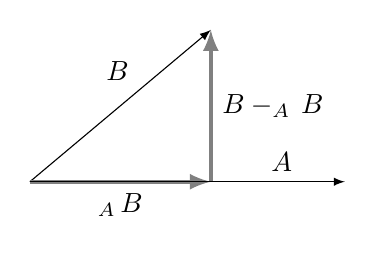
\begin{tikzpicture}
\pgfmathsetmacro{\ang}{40}
\pgfmathsetmacro{\len}{3}
\pgfmathsetmacro{\kx}{\len*cos(\ang)}
\draw[-latex](0,0)--++(\ang:\len)coordinate(k)node[pos=0.6,above left]{$\kvec{B}$};
\draw[-latex,ultra thick,gray](\kx,0)--(k)node[pos=0.5,right,black]{$\kvec{B}-\proj_{\kvec{A}}\,\kvec{B}$};
\draw[-latex,ultra thick,gray](0,0)--(\kx,0)node[pos=0.5,below,black]{$\proj_{\kvec{A}}\,\kvec{B}$};
\draw[-latex](0,0)--(4,0)node[pos=0.8,above]{$\kvec{A}$};
\RightAngle{(k)}{(\kx,0)}{(4,0)}
\end{tikzpicture}
\caption{سمتیہ \عددی{\kvec{B}} کو سمتیہ \عددی{\kvec{A}} کے عمودی اور متوازی سمتیات کا مجموعہ لکھنا۔}
\label{شکل_سمتیہ_عمودی_متوازی_مجموعہ}
\end{figure}

\ابتدا{مثال}
سمتیہ \عددی{\kvec{B}=2\ai+\aj-3\ak} کو سمتیہ \عددی{\kvec{A}=3\ai-\aj} کے متوازی سمتیہ اور \عددی{\kvec{A}} کے عمودی سمتیہ کا مجموعہ لکھیں۔

حل:\quad
ہم درج ذیل 
\begin{align*}
\kvec{A}\cdot\kvec{B}=6-1=5,\quad \kvec{A}\cdot\kvec{A}=9+1=10
\end{align*}
کو مساوات \حوالہ{مساوات_سمتیہ_متوازی_عمودی_مجموعہ} میں پر کرتے ہیں۔
\begin{align*}
\kvec{B}=\frac{\kvec{B}\cdot\kvec{A}}{\kvec{A}\cdot\kvec{A}}\kvec{A}+\big(\kvec{B}-\frac{\kvec{B}\cdot\kvec{A}}{\kvec{A}\cdot\kvec{A}}\kvec{A}\big)&=\frac{5}{10}(3\ai-\aj)+\big(2\ai+\aj-3\ak-\frac{5}{10}(3\i-\aj)\big)\\
&=\big(\frac{3}{2}\ai-\frac{1}{2}\aj\big)+\big(\frac{1}{2}\ai+\frac{3}{2}\aj-3\ak\big)
\end{align*}
آپ تسلی کر لیں کہ دائیں ہاتھ پہلا جزو \عددی{\tfrac{1}{2}\kvec{A}} کے برابر ہے۔دائیں ہاتھ دوسرا جزو درج ذیل کی بنا \عددی{\kvec{A}} کو عمودی ہے۔
\begin{align*}
\big(\frac{1}{2}\ai+\frac{3}{2}\aj-3\ak\big)\cdot (3\ai-\aj)=\frac{3}{2}-\frac{3}{2}=0
\end{align*}
\انتہا{مثال}
%==============

\جزوحصہء{کام}
ہم نے حصہ \حوالہ{حصہ_تکمل_استعمال_کام} میں مستقل قوت \عددی{F} جو ایک جسم پر عمل کر کے اس کو قوت کے رخ  \عددی{d} فاصلہ منتقل کرتی  ہے کا کام کلیہ \عددی{W=Fd} سے دریافت کیا۔ یہ کلیہ صرف اس صورت درست ہو گا جب قوت کا رخ اور حرکت کا رخ ایک ہوں۔ اگر مستقل قوت \عددی{\kvec{F}} اور جسم کے ہٹاو \عددی{\kvec{D}=\krightharpoonup{NQ}} کے رخ مختلف ہوں تب \عددی{\kvec{D}} کے رخ،  \عددی{\kvec{F}} کا جزو کام کرے گا۔ اگر \عددی{\kvec{F}} اور \عددی{\kvec{D}} کے بیچ زاویہ \عددی{\theta} ہو تب  کام درج ذیل ہو گا (شکل \حوالہ{شکل_سمتیہ_کام_کی_تعریف})۔
\begin{align*}
\text{کام}&=(\text{\RL{\عددی{\kvec{D}} کے رخ \عددی{\kvec{F}} کا غیر سمتی جزو}})(\text{\RL{\عددی{\kvec{D}} کی لمبائی}})\\
&=(\abs{\kvec{F}}\cos\theta)\abs{\kvec{D}}\\
&=\kvec{F}\cdot\kvec{D}
\end{align*} 

\begin{figure}
\centering
\begin{tikzpicture}
\pgfmathsetmacro{\d}{1.5}
\pgfmathsetmacro{\f}{2}
\pgfmathsetmacro{\ang}{30}
\draw[-latex](0,0)node[circ]{}node[above]{$N$}--(\d,0)node[above]{$Q$}node[pos=0.5,above]{$\kvec{D}$};
\draw[-latex](\d,0)node[circ]{}--++(\ang:\f)node[pos=0.5,above]{$\kvec{F}$}coordinate(a);
\draw[dashed](a)--($(0,0)!(a)!(3,0)$)coordinate(b)--(\d,0);
\draw[stealth-stealth] ($(b)+(0,-0.3)$)--($(\d,0)+(0,-0.3)$)node[pos=0.5,below]{$\abs{\kvec{F}}\cos\theta$};
\draw(b)++(0,-0.2)--++(0,-0.2);
\draw(\d,-0.2)--++(0,-0.2);
\draw([shift={(0:0.5)}]\d,0) arc (0:\ang:0.5)node[pos=0.7,right]{$\theta$};
\end{tikzpicture}
\caption{ہٹاو \عددی{\kvec{D}} کے دوران مستقل قوت \عددی{\kvec{F}} کا کام \عددی{(\abs{\kvec{F}}\cos\theta)\abs{\kvec{D}}} ہو گا۔}
\label{شکل_سمتیہ_کام_کی_تعریف}
\end{figure}

\ابتدا{تعریف}
ہٹاو \عددی{\kvec{D}=\krightharpoonup{NQ}} کے دوران مستقل قوت \عددی{\kvec{F}} کا کام
\begin{align}\label{مساوات_سمتیہ_کام_کی_تعریف}
W=\kvec{F}\cdot\kvec{D}=\abs{\kvec{F}}\abs{\kvec{D}}\cos\theta
\end{align}
ہو گا جہاں ہٹاو اور قوت کے بیچ زاویہ \عددی{\theta} ہے۔
\انتہا{تعریف}
%====================

کام کی اکائی نیوٹن ضرب میٹر ہے جس کو عموماً \اصطلاح{جاول}\فرہنگ{جاول}\حاشیہب{joule}\فرہنگ{joule} کہتے ہیں۔

\ابتدا{مثال}
اگر \عددی{\abs{\kvec{F}}=\SI{40}{\newton}} اور \عددی{\abs{\kvec{D}}=\SI{3}{\meter}} ہوں اور \عددی{\theta=60^{\circ}} ہو تب کام درج ذیل ہو گا۔
\begin{align*}
\text{کام}&=\abs{\kvec{F}}\abs{\kvec{D}}\cos\theta\\
&=(40)(3)\cos 60^{\circ}\\
&=(120)(\tfrac{1}{2})\\
&=\SI{60}{\joule}
\end{align*}
\انتہا{مثال}
%===================

\حصہء{سوالات}
سوال \حوالہ{سوال_سمتیہ_غیر_سمتی_الف} تا سوال \حوالہ{سوال_سمتیہ_غیر_سمتی_ب} میں درج ذیل دریافت کریں۔
\begin{enumerate}[a.]
\item
\عددی{\kvec{A}\cdot\kvec{B}}، \عددی{\abs{\kvec{A}}}، \عددی{\abs{\kvec{B}}}
\item
\عددی{\kvec{A}} اور \عددی{\kvec{B}} کے بیچ زاویہ کا کوسائن۔
\item
\عددی{\kvec{A}} کے رخ \عددی{\kvec{B}} کا غیر سمتی جزو۔
\item
سمتیہ \عددی{\proj_{\kvec{A}}\,\kvec{B}}
\end{enumerate}

\ابتدا{سوال}\شناخت{سوال_سمتیہ_غیر_سمتی_الف}
$\kvec{A}=2\ai-4\aj+\sqrt{5}\ak,\quad \kvec{B}=-2\ai+4\aj-\sqrt{5}\ak$\\
جواب:\quad
(ا) \عددی{-25,\, 5,\,5}، (ب) \عددی{-1}، (ج) \عددی{-5}، (د) \عددی{-2\ai+4\aj-\sqrt{5}\ak}
\انتہا{سوال}
%===================
\ابتدا{سوال}
$\kvec{A}=\tfrac{3}{5}\ai+\tfrac{4}{5}\ak,\quad \kvec{B}=5\ai+12\aj$
\انتہا{سوال}
%==================
\ابتدا{سوال}
$\kvec{A}=10\ai+11\aj-2\ak,\quad \kvec{B}=3\aj+4\ak$\\
جواب:\quad
(ا) \عددی{25,\,15,\,5}، (ب) \عددی{\tfrac{1}{3}}، (ج) \عددی{\tfrac{5}{3}}، (د) \عددی{\tfrac{1}{9}(10\ai+11\aj-2\ak)}
\انتہا{سوال}
%==================
\ابتدا{سوال}
$\kvec{A}=2\ai+10\aj-11\ak,\quad \kvec{B}=2\ai+2\aj+\ak$
\انتہا{سوال}
%==================
\ابتدا{سوال}
$\kvec{A}=-2\ai+7\aj,\quad \kvec{B}=\ak$\\
جواب:\quad
(ا) \عددی{0,\,\sqrt{53}}، (ب) \عددی{0}، (ج) \عددی{0}، (د) \عددی{0}
\انتہا{سوال}
%==================
\ابتدا{سوال}
$\kvec{A}=\tfrac{1}{\sqrt{2}}\ai+\tfrac{1}{\sqrt{3}}\aj+\tfrac{1}{\sqrt{6}}\ak,\quad \kvec{B}=\tfrac{1}{\sqrt{2}}\aj-\ak$
\انتہا{سوال}
%==================
\ابتدا{سوال}
$\kvec{A}=5\aj-3\ak,\quad \kvec{B}=\ai+\aj+\ak$\\
جواب:\quad
(ا) \عددی{2,\,\sqrt{34},\,\sqrt{3}}، (ب) \عددی{\tfrac{2}{\sqrt{3}\sqrt{34}}}، (ج) \عددی{\tfrac{2}{\sqrt{34}}}، (د) \عددی{\tfrac{1}{17}(5\aj-3\ak)}
\انتہا{سوال}
%==================
\ابتدا{سوال}
$\kvec{A}=\ai+\ak,\quad \kvec{B}=\ai+\aj+\ak$
\انتہا{سوال}
%==================
\ابتدا{سوال}
$\kvec{A}=-\ai+\aj,\quad \kvec{B}=\sqrt{2}\ai+\sqrt{3}\aj+2\ak$\\
جواب:\quad
(ا) \عددی{\sqrt{3}-\sqrt{2},\,\sqrt{2},\,3}، (ب) \عددی{\tfrac{\sqrt{3}-\sqrt{2}}{3\sqrt{2}}}، (ج) \عددی{\tfrac{\sqrt{3}-\sqrt{2}}{\sqrt{2}}}، (د) \عددی{\tfrac{\sqrt{3}-\sqrt{2}}{2}(-\ai+\aj)}
\انتہا{سوال}
%==================
\ابتدا{سوال}\شناخت{سوال_سمتیہ_غیر_سمتی_ب}
$\kvec{A}=-5\ai+\aj,\quad \kvec{B}=2\ai+\sqrt{17}\aj+10\ak$
\انتہا{سوال}
%==================

\ابتدا{سوال}
سمتیہ \عددی{\kvec{B}=3\aj+4\ak} کو سمتیہ \عددی{\kvec{A}=\ai+\aj} کے عمودی سمتیہ اور \عددی{\kvec{A}} کے متوازی سمتیہ کا مجموعہ لکھیں۔\\
جواب:\quad
$(\tfrac{3}{2}\ai+\tfrac{3}{2}\aj)+(-\tfrac{3}{2}\ai+\tfrac{3}{2}\aj+4\ak)$
\انتہا{سوال}
%=====================
\ابتدا{سوال}
سمتیہ \عددی{\kvec{B}=\aj+\ak} کو سمتیہ \عددی{\kvec{A}=\ai+\aj} کے عمودی سمتیہ اور \عددی{\kvec{A}} کے متوازی سمتیہ کا مجموعہ لکھیں۔
\انتہا{سوال}
%=====================
\ابتدا{سوال}
سمتیہ \عددی{\kvec{B}=8\ai+4\aj-12\ak} کو سمتیہ \عددی{\kvec{A}=\ai+2\aj-\ak} کے عمودی سمتیہ اور \عددی{\kvec{A}} کے متوازی سمتیہ کا مجموعہ لکھیں۔\\
جواب:\quad
$(\tfrac{14}{3}\ai+\tfrac{28}{3}\aj-\tfrac{14}{3}\ak)+(\tfrac{10}{3}\ai-\tfrac{16}{3}\aj-\tfrac{22}{3}\ak)$
\انتہا{سوال}
%=====================
\ابتدا{سوال}
سمتیہ \عددی{\kvec{B}=\ai+(\aj+\ak)} پہلے سے سمتیہ \عددی{\ai} کے متوازی سمتیہ اور \عددی{\ai} کے عمودی سمتیہ کا مجموعہ ہے۔  اگر مساوات \حوالہ{مساوات_سمتیہ_متوازی_عمودی_مجموعہ} میں \عددی{\kvec{A}=\ai} ہو تب کیا \عددی{\kvec{B}_{\parallel,\kvec{A}}=\ai} اور \عددی{\kvec{B}_{\perp,\kvec{A}}=\aj+\ak} ملتے ہیں۔ (متوازی اور عمودی اجزاء کو بالترتیب زیر نوشت \عددی{\parallel} اور \عددی{\perp} سے ظاہر کیا جاتا ہے۔)
\انتہا{سوال}
%==================

\موٹا{جیومیٹری}\\
\ابتدا{سوال}\شناخت{سوال_سمتیہ_جیومیٹری_فرق_مجموعہ_الف}
\ترچھا{مجموعات اور فرق۔}\quad
ایسا معلوم ہوتا ہے کہ شکل \حوالہ{شکل_سوال_سمتیہ_جیومیٹری_فرق_مجموعہ_الف} میں \عددی{\kvec{v}_1+\kvec{v}_2} اور \عددی{\kvec{v}_1-\kvec{v}_2} عمودی ہیں۔ کیا یہ محض ایک اتفاق ہے یا ہم توقع کر سکتے ہیں کہ کسی بھی دو سمتیات کا مجموعہ اور فرق عمودی ہوں گے؟ اپنے جواب کی وجہ پیش کریں۔\\
جواب:\quad
یکساں مقدار کے دو سمتیات کا مجموعہ اور تفریق ہر صورت ایک دوسرے کے عمودی  ہوتے ہیں۔ یہ حقیقت درج ذیل سے واضح ہو گا۔
\begin{align*}
(\kvec{v}_1-\kvec{v}_2)\cdot(\kvec{v}_1+\kvec{v}_2)=\kvec{v}_1\cdot\kvec{v}_1+\kvec{v}_1\cdot\kvec{v}_2-\kvec{v}_2\cdot\kvec{v}_1-\kvec{v}_2\cdot\kvec{v}_2=\abs{\kvec{v}_1}^2-\abs{\kvec{v}_2}^2
\end{align*}
\انتہا{سوال}
%==========
\ابتدا{سوال}\شناخت{سوال_سمتیہ_دائرہ_پر_نقطہ}
ایک دائرہ جس کا مرکز \عددی{O}  ہے کا قطر \عددی{AB} ہے۔ نقطہ \عددی{C} دائرے پر پایا جاتا ہے (شکل \حوالہ{شکل_سوال_سمتیہ_دائرہ_پر_نقطہ})۔ دکھائیں کہ \عددی{\krightharpoonup{CA}} اور \عددی{\krightharpoonup{CB}} عمودی ہوں گے۔
\انتہا{سوال}
%======================
\begin{figure}
\centering
\begin{minipage}{0.30\textwidth}
\centering
\begin{tikzpicture}
\pgfmathsetmacro{\da}{1.5}
\pgfmathsetmacro{\a}{30}
\pgfmathsetmacro{\db}{1.5}
\pgfmathsetmacro{\b}{90}
\draw[-latex](0,0)--++(\a:\da)coordinate(ka)node[pos=0.5,above]{$\kvec{v}_1$};
\draw[-latex](ka)--++(\b:\db)coordinate(kb)node[pos=0.5,right]{$\kvec{v}_2$};
\draw[-latex](ka)--++(-\b:\db)coordinate(kc)node[pos=0.5,right]{$-\kvec{v}_2$};
\draw[-latex](0,0)--(kb)node[pos=0.5,sloped, above]{$\kvec{v}_1+\kvec{v}_2$};
\draw[-latex](0,0)--(kc)node[pos=0.5,sloped,below]{$\kvec{v}_1-\kvec{v}_2$};
\end{tikzpicture}
\caption{سمتیات برائے سوال \حوالہ{سوال_سمتیہ_جیومیٹری_فرق_مجموعہ_الف}}
\label{شکل_سوال_سمتیہ_جیومیٹری_فرق_مجموعہ_الف}
\end{minipage}\hfill
\begin{minipage}{0.30\textwidth}
\centering
\begin{tikzpicture}
\pgfmathsetmacro{\r}{1.5}
\draw(0,0)node[circ]{}node[below]{$O$}circle (\r);
\draw[-latex](0,0)--(\r,0)node[right]{$B$}node[pos=0.5,below]{$\kvec{u}$};
\draw[-latex](0,0)--(-\r,0)node[left]{$A$}node[pos=0.5,below]{$-\kvec{u}$};
\draw[-latex](0,0)--++(140:\r)node[above]{$C$}node[pos=0.5,right]{$\kvec{v}$};
\end{tikzpicture}
\caption{دائرہ برائے سوال \حوالہ{سوال_سمتیہ_دائرہ_پر_نقطہ}}
\label{شکل_سوال_سمتیہ_دائرہ_پر_نقطہ}
\end{minipage}\hfill
\begin{minipage}{0.30\textwidth}
\centering
\begin{tikzpicture}
\pgfmathsetmacro{\len}{2}
\pgfmathsetmacro{\ang}{30}
\pgfmathsetmacro{\angX}{-130}
%\draw[-latex](0,0)node[left]{$O$}--(-1.25,-1.25)node[below]{$x$};
\draw[-latex](0,0)node[left]{$O$}--++(\angX:1.5)node[below]{$x$};
\draw[-latex](0,0)--(2.5,0)node[right]{$y$};
\draw[-latex](0,0)--(0,1.75)node[above]{$z$};
\draw[-latex,thick](0,0)--++(\ang:\len)coordinate(kt)node[pos=0.65,above]{$\kvec{v}$};
\draw(kt)--(2,0);
\draw(kt)--(0,1.25);
\draw(kt)--(\angX:1)coordinate(kk);
\RightAngle{(kt)}{(2,0)}{(0,0)}
\RightAngle{(kt)}{(0,1.25)}{(0,0)}
\RightAngle{(kt)}{(kk)}{(\angX:1.25)}
\draw[-stealth]([shift={(90:0.5)}]0,0) arc (90:\ang:0.5)node[pos=0.6,above]{$\gamma$};
\draw[-stealth]([shift={(0:0.8)}]0,0) arc (0:\ang:0.8)node[pos=0.6,right]{$\beta$};
\draw[-stealth](\angX:0.3) to [out=20,in=-100]node[pos=0.3,below,xshift=1ex]{$\alpha$}(\ang:0.3);
\end{tikzpicture}
\caption{زاویات رخ اور کوسائن رخ کی تعریف برائے سوال \حوالہ{سوال_سمتیہ_کوسائن_رخ}۔}
\label{شکل_سوال_سمتیہ_کوسائن_رخ}
\end{minipage}

\end{figure}

\ابتدا{سوال}
دکھائیں کہ یکساں اضلاع کے متوازی الاضلاع کے وتر ایک دوسرے کے عمودی ہوتے ہیں۔ 
\انتہا{سوال}
%========
\ابتدا{سوال}
دکھائیں کہ مربع وہ واحد مستطیل ہے جس کے وتر عمودی ہوتے ہیں۔
\انتہا{سوال}
%===============
\ابتدا{سوال}
ثابت کریں کہ ایک متوازی الاضلاع صرف اور صرف اس صورت مستطیل ہو گا جب اس کے وتروں  کی لمبائی ایک جیسی ہو۔ ترکھان اس حقیقت کو عموماً استعمال کرتا ہے۔
\انتہا{سوال}
%==========
\ابتدا{سوال}
متوازی الاضلاع کے قریبی ضلع \عددی{\kvec{u}} اور \عددی{\kvec{v}} ہیں۔ دکھائیں کہ ان کے مشترکہ راس سے مخالف راس تک وتر، سمتیات  \عددی{\kvec{u}} اور \عددی{\kvec{v}} کے بیچ زاویہ کو دو برابر حصوں میں تقسیم کرتا ہے۔ 
\انتہا{سوال}
%=============
\ابتدا{سوال}
ایک اہرام کے مربع قاعدہ \عددی{OABC} کے ضلع  کی لمبائی \عددی{1} اکائی ہے  اور اہرام کی چوٹی \عددی{D} ہے۔اہرام کا قد بھی \عددی{1} اکائی ہے۔ یوں نقطہ  \عددی{D} ٹھیک وتر \عددی{OB} کے وسطی نقطہ کے سیدھا اوپر  ہو گا۔ قطع \عددی{\krightharpoonup{OB}} اور \عددی{\krightharpoonup{OD}} کے بیچ زاویہ تلاش کریں۔\\
جواب:\quad
$\tan^{-1}\sqrt{2}$
\انتہا{سوال}
%===================
\ابتدا{سوال}\شناخت{سوال_سمتیہ_کوسائن_رخ}\ترچھا{زاویات رخ اور کوسائن رخ}\\
سمتیہ \عددی{\kvec{v}=a\ai+b\aj+c\ak} کے زاویات رخ \عددی{\alpha}، \عددی{\beta} اور \عددی{\gamma} کی تعریف درج ذیل ہے (شکل \حوالہ{شکل_سوال_سمتیہ_کوسائن_رخ})۔
\begin{enumerate}[]
\item
مثبت محور \عددی{x} اور \عددی{\kvec{v}} کے بیچ زاویہ \عددی{\alpha} ہے (\عددی{0\le\alpha\le\pi})،
\item
مثبت محور \عددی{y} اور \عددی{\kvec{v}} کے بیچ زاویہ \عددی{\beta} ہے (\عددی{0\le\beta\le\pi})،
\item
مثبت محور \عددی{z} اور \عددی{\kvec{v}} کے بیچ زاویہ \عددی{\gamma} ہے (\عددی{0\le\gamma\le\pi})۔
\end{enumerate}
\begin{enumerate}[a.]
\item
درج ذیل
\begin{align*}
\cos\alpha=\frac{a}{\abs{\kvec{v}}},\quad \cos\beta=\frac{b}{\abs{\kvec{v}}},\quad \cos\gamma=\frac{c}{\abs{\kvec{v}}}
\end{align*} 
اور \عددی{\cos^2\alpha+\cos^2\beta+\cos^2\gamma=1} دکھائیں۔ ان کوسائن کو \اصطلاح{کوسائن رخ}\فرہنگ{کوسائن!رخ}\حاشیہب{direction cosines}\فرہنگ{direction!cosines} کہتے ہیں۔
\item
\ترچھا{کوسائن رخ اور اکائی سمتیات۔} دکھائیں کہ اگر \عددی{\kvec{v}=a\ai+b\aj+c\ak} ایک اکائی سمتیہ ہو تب \عددی{a}، \عددی{b} اور \عددی{c} سمتیہ \عددی{\kvec{v}} کے کوسائن رخ ہوں گے۔
\end{enumerate}
\انتہا{سوال}
%======================

\موٹا{سمتیات کے بیچ زاویے}\\
سوال \حوالہ{سوال_سمتیہ_زاویات_بیچ_سمتیات_الف} تا سوال \حوالہ{سوال_سمتیہ_زاویات_بیچ_سمتیات_ب} میں کیلکولیٹر کی مدد سے سمتیات کے بیچ زاویات کو، ایک فی صد درست، ریڈیئن میں  تلاش کریں۔

\ابتدا{سوال}\شناخت{سوال_سمتیہ_زاویات_بیچ_سمتیات_الف}
$\kvec{A}=2\ai+\aj,\quad \kvec{B}=\ai+2\aj-\ak$\\
جواب:\quad
\عددی{0.75} ریڈیئن
\انتہا{سوال}
%===================
\ابتدا{سوال}
$\kvec{A}=2\ai-2\aj+\ak,\quad \kvec{B}=3\ai+4\ak$
\انتہا{سوال}
%===================
\ابتدا{سوال}
$\kvec{A}=\sqrt{3}\ai-7\aj,\quad \kvec{B}=\sqrt{3}\ai+\aj-2\ak$\\
جواب:\quad
\عددی{1.77} ریڈیئن
\انتہا{سوال}
%===================
\ابتدا{سوال}\شناخت{سوال_سمتیہ_زاویات_بیچ_سمتیات_ب}
$\kvec{A}=\ai+\sqrt{2}\aj-\sqrt{2}\ak,\quad \kvec{B}=-\ai+\aj+\ak$
\انتہا{سوال}
%===================

سوال \حوالہ{سوال_سمتیہ_زاویات_بیچ_الف} تا سوال \حوالہ{سوال_سمتیہ_زاویات_بیچ_ب} میں کیلکولیٹر کی مدد سے سمتیات کے بیچ زاویات کو، ایک فی صد درست، ریڈیئن میں  تلاش کریں۔

\ابتدا{سوال}\شناخت{سوال_سمتیہ_زاویات_بیچ_الف}
مثلث \عددی{ABC} کے اندرونی زاویات۔ مثلث کے راس \عددی{A(-1,0,2)}، \عددی{B(2,1,-1)} اور \عددی{C(1,-2,2)} ہیں۔\\
جواب:\quad
$\phase{A}\approx 1.24,\,\phase{B}\approx 0.66,\,\phase{C}\approx 1.24$
\انتہا{سوال}
%=====================
\ابتدا{سوال}
سمتیات \عددی{\kvec{A}=2\ai+2\aj+\ak} اور \عددی{\kvec{B}=2\ai+10\aj-11\ak} کے بیچ زاویہ۔
\انتہا{سوال}
%====================
\ابتدا{سوال}\شناخت{سوال_سمتیہ_زاویات_بیچ_ب}
مکعب کے وتر اور مکعب کی ایک سطح کے وتر کے بیچ زاویہ۔ (اشارہ: ایسا مکعب استعمال کریں جس کے کنارے \عددی{\ai}، \عددی{\aj} اور \عددی{\ak} ہوں۔)\\
جواب:\quad
\عددی{0.62} ریڈیئن
\انتہا{سوال}
%====================
\ابتدا{سوال}
پانی کی نالی میں ایک جوڑ ہے۔اس جوڑ سے  شمال رخ نالی کی ڈھلوان \عددی{\SI{10}{\percent}} ہے جبکہ جوڑ سے مشرق رخ نالی کی ڈھلوان \عددی{\SI{20}{\percent}} ہے۔ اس جوڑ پر نالی کے دو حصوں کے بیچ زاویہ کتنا ہو گا؟
\انتہا{سوال}
%==================

\موٹا{نظریہ اور مثالیں}\\
\ابتدا{سوال}
\begin{enumerate}[a.]
\item
کسی بھی سمتیات \عددی{\kvec{u}} اور \عددی{\kvec{v}} کے لئے عدم مساوات \عددی{\abs{\kvec{u}\cdot\kvec{v}}\le \abs{\kvec{u}}\abs{\kvec{v}}} کو \عددی{\kvec{u}\cdot\kvec{v}=\abs{\kvec{u}}\abs{\kvec{v}}\cos\theta} کی مدد سے دکھائیں۔
\item
کیا کبھی \عددی{\abs{\kvec{u}\cdot\kvec{v}}=\abs{\kvec{u}}\abs{\kvec{v}}} ہو سکتا ہے؟ اگر ہو سکتا ہے تب کب ایسا ہو گا؟  اپنے جواب کی وجہ پیش کریں۔
\end{enumerate}
جواب:\quad
(ا) چونکہ \عددی{\abs{\cos\theta}\le 1}  ہوتا ہے لہٰذا 
$\abs{\kvec{u}\cdot\kvec{v}}=\abs{\kvec{u}}\abs{\kvec{v}}\abs{\cos\theta}\le\abs{\kvec{u}}\abs{\kvec{v}}(1)=\abs{\kvec{u}}\abs{\kvec{v}}$
ہو گا۔ (ب) جب \عددی{\abs{\cos \theta}=1} ہو یا \عددی{\kvec{u}} اور \عددی{\kvec{v}} میں سے ایک یا دونوں صفر ہوں۔ غیر صفر سمتیات کی صورت میں مساوات تب درست ہو گا جب سمتیات متوازی ہوں یعنی جب \عددی{\theta=0} یا \عددی{\theta=\pi} ہو۔
\انتہا{سوال}
%=========
\ابتدا{سوال}
مستوی \عددی{xy} میں عمومی سمتیہ \عددی{\kvec{v}} بنائیں۔ اب ان نقطوں \عددی{(x,y)} کی نشاندہی کریں جن پر \عددی{(x\ai+y\aj)\cdot \kvec{v}=0} ہو گا۔ اپنے جواب کی وجہ پیش کریں۔
\انتہا{سوال}
%===============
\ابتدا{سوال}
اگر \عددی{\kvec{u}_1} اور \عددی{\kvec{u}_2} عمودی اکائی سمتیات ہوں اور \عددی{\kvec{v}=a\kvec{u}_1+b\kvec{u}_2} ہو تب \عددی{\kvec{v}\cdot\kvec{u}_1} تلاش کریں۔\\
جواب:\quad
$a $
\انتہا{سوال}
%===================
\ابتدا{سوال}\ترچھا{ضرب نقطہ میں مشترک اجزاء کی منسوخی}\\
حقیقی اعداد کے ضرب میں اگر \عددی{ab_1=ab_2} ہو اور \عددی{a} غیر صفر ہو تب دونوں اطراف \عددی{a} کو منسوخ کر کے \عددی{b_1=b_2} لکھا جا سکتا ہے۔ کیا ضرب نقطہ میں ایسا کرنا ممکن ہو گا: یعنی اگر \عددی{\kvec{A}\cdot\kvec{B}_1=\kvec{A}\cdot\kvec{B}_2} ہو تب کیا دونوں اطراف \عددی{\kvec{A}} منسوخ کر کے \عددی{\kvec{B}_1=\kvec{B}_2} لکھا جا سکتا ہے؟۔ اپنے جواب کی وجہ پیش کریں۔
\انتہا{سوال}
%====================
\ابتدا{سوال}
فرض کریں \عددی{\kvec{A}}، \عددی{\kvec{B}} اور \عددی{\kvec{C}} آپس میں عمودی سمتیات ہیں۔ اب \عددی{\kvec{D}=5\kvec{A}-6\kvec{B}+3\kvec{C}} لیں۔
\begin{enumerate}[a.]
\item
اگر \عددی{\kvec{A}}، \عددی{\kvec{B}} اور \عددی{\kvec{C}} اکائی سمتیات ہوں تب \عددی{\kvec{D}} کی مقدار \عددی{\abs{\kvec{D}}} تلاش کریں۔
\item
اگر \عددی{\abs{\kvec{A}}=2}، \عددی{\abs{\kvec{B}}=3} اور \عددی{\abs{\kvec{C}}=4} ہوں تب \عددی{\abs{\kvec{D}}} کتنا ہو گا؟
\end{enumerate}
جواب:\quad
(ا) \عددی{\sqrt{70}}، (ب) \عددی{\sqrt{568}}
\انتہا{سوال}
%==========
\ابتدا{سوال}
فرض کریں \عددی{\kvec{A}}، \عددی{\kvec{B}} اور \عددی{\kvec{C}} آپس میں عمودی اکائی سمتیات ہیں۔ اگر \عددی{\kvec{D}=\alpha\kvec{A}+\beta\kvec{B}+\gamma\kvec{C}} ہو جہاں \عددی{\alpha}، \عددی{\beta} اور \عددی{\gamma} غیر سمتی ہیں تب دکھائیں کہ \عددی{\alpha=\kvec{D}\cdot\kvec{A}}، \عددی{\beta=\kvec{D}\cdot\kvec{B}} اور \عددی{\gamma=\kvec{D}\cdot\kvec{C}} ہوں گے۔ 
\انتہا{سوال}
%===================

\موٹا{کام}\\
\ابتدا{سوال}
قوت \عددی{\kvec{F}=5\ak} (مقدار \عددی{5} نیوٹن) سیدھی لکیر پر مبدا سے نقطہ \عددی{(1,1,1)} تک  ایک جسم کو منتقل کرتا ہے (فاصلہ میٹر میں ہے)۔ یہ قوت کتنا کام کرتی ہے؟\\
جواب:\quad
\عددی{\SI{5}{\joule}}
\انتہا{سوال}
%============
\ابتدا{سوال}
ایک ریل گاڑی کا انجن \عددی{6000} ٹن کمیت کی ریل گاڑی کو \عددی{\SI{602148}{\newton}} قوت سے کھینچ سکتا ہے۔ ایک افقی سیدھی پٹڑی پر \عددی{605} کلو میٹر فاصلہ طے کر کے یہ انجن کتنا کام کرتا ہے؟
\انتہا{سوال}
%======================
\ابتدا{سوال}
ایک بوجھ کو \عددی{\SI{20}{\meter}} لمبی ڈھلوان پر \عددی{\SI{200}{\newton}} قوت کھینچتی ہے۔افقی سطح کے ساتھ یہ قوت \عددی{30^{\circ}} کا زاویہ بناتی ہے۔ یہ قوت کتنا کام کرتی ہے؟ \\
جواب:\quad
$\SI{3464.10}{\joule}$
\انتہا{سوال}
%================
\ابتدا{سوال}
ایک کشتی کے  بادبان پر ہوا \عددی{\SI{2000}{\newton}} قوت لگاتی ہے۔ افقی سطح کے ساتھ قوت کا زاویہ \عددی{60^{\circ}} ہے۔ ایک کلومیٹر فاصل طے کرنے میں یہ قوت کتنا کام کرتی ہے؟
\انتہا{سوال}
%===================

\موٹا{مستوی میں خط کی مساواتیں}\\
\ابتدا{سوال}\شناخت{سوال_سمتیہ_لکیر_عمودی_سمتیہ}
دکھائیں کہ سمتیہ \عددی{\kvec{v}=a\ai+b\aj} لکیر \عددی{ax+by=c} کو عمودی ہے۔ ایسا کرنے کی خاطر دکھائیں کہ اس لکیر کی ڈھلوان، اس سمتیہ کی ڈھلوان کے بالعکس متناسب کا نفی ہے۔
\انتہا{سوال}
%==========================
\ابتدا{سوال}\شناخت{سوال_سمتیہ_لکیر_متوازی_سمتیہ}
دکھائی کہ سمتیہ \عددی{\kvec{v}=a\ai+b\aj} لکیر \عددی{bx-ay=c} کے متوازی ہے۔ ایسا کرنے کی خاطر دکھائیں کہ لکیر کی ڈھلوان اور سمتیہ کی ڈھلوان ایک دوسرے جیسے  ہیں۔
\انتہا{سوال}
%====================

سوال \حوالہ{سوال_سمتیہ_عمودی_خط_الف} تا سوال \حوالہ{سوال_سمتیہ_عمودی_خط_پ} میں سوال \حوالہ{سوال_سمتیہ_لکیر_عمودی_سمتیہ} کا نتیجہ استعمال کر کے نقطہ \عددی{N} پر  \عددی{\kvec{v}} کے عمودی خط کی مساوات دریافت کریں۔ اس لکیر کو ترسیم کر کے مبدا پر اس عمودی سمتیہ کا بھی خاکہ بنائیں۔

\ابتدا{سوال}\شناخت{سوال_سمتیہ_عمودی_خط_الف}
$N(2,1),\quad \kvec{v}=\ai+2\aj$\\
جواب:\quad
$x+2y=4$\quad
شکل \حوالہ{شکل_سوال_سمتیہ_عمودی_خط_الف}
\انتہا{سوال}
%====================== 
\ابتدا{سوال}
$N(-1,2),\quad \kvec{v}=-2\ai-\aj$
\انتہا{سوال}
%====================== 
\ابتدا{سوال}\شناخت{سوال_سمتیہ_عمودی_خط_ب}
$N(-2,-7),\quad \kvec{v}=-2\ai+\aj$\\
جواب:\quad
$-2x+y=-3$\quad
شکل \حوالہ{شکل_سوال_سمتیہ_عمودی_خط_ب}
\انتہا{سوال}
%====================== 
\ابتدا{سوال}\شناخت{سوال_سمتیہ_عمودی_خط_پ}
$N(11,10),\quad \kvec{v}=2\ai-3\aj$
\انتہا{سوال}
%====================== 


سوال \حوالہ{سوال_سمتیہ_متوازی_خط_الف} تا سوال \حوالہ{سوال_سمتیہ_متوازی_خط_پ} میں سوال \حوالہ{سوال_سمتیہ_لکیر_متوازی_سمتیہ} کا نتیجہ استعمال کر کے نقطہ \عددی{N} پر  \عددی{\kvec{v}} کے متوازی خط کی مساوات دریافت کریں۔ اس لکیر کو ترسیم کر کے مبدا پر اس متوازی سمتیہ کا بھی خاکہ بنائیں۔

\ابتدا{سوال}\شناخت{سوال_سمتیہ_متوازی_خط_الف}
$N(-2,1),\quad \kvec{v}=\ai-\aj$\\
جواب:\quad
$x+y=-1$\quad
شکل \حوالہ{شکل_سوال_سمتیہ_متوازی_خط_الف}
\انتہا{سوال}
%=========================
\ابتدا{سوال}
$N(0,-2),\quad \kvec{v}=2\ai+3\aj$
\انتہا{سوال}
%=========================
\ابتدا{سوال}\شناخت{سوال_سمتیہ_متوازی_خط_ب}
$N(1,2),\quad \kvec{v}=-\ai-2\aj$\\
جواب:\quad
$2x-y=0$\quad
شکل \حوالہ{شکل_سوال_سمتیہ_متوازی_خط_ب}
\انتہا{سوال}
%=========================
\ابتدا{سوال}\شناخت{سوال_سمتیہ_متوازی_خط_پ}
$N(1,3),\quad \kvec{v}=3\ai-2\aj$
\انتہا{سوال}
%=========================

\موٹا{مستوی میں خطوط کے بیچ زاویے}\\
دو مستوی خط جن کے بیچ زاویہ حادہ جو قائمہ نہ ہو  وہی ہو گا جو ان خطوط کے عمودی دو سمتیات کے بیچ یا ان خطوط کے متوازی دو سمتیات کے بیچ ہو گا۔اس حقیقت کے ساتھ  سوال \حوالہ{سوال_سمتیہ_لکیر_عمودی_سمتیہ} یا سوال \حوالہ{سوال_سمتیہ_لکیر_متوازی_سمتیہ} کا نتیجہ استعمال کرتے ہوئے  سوال \حوالہ{سوال_سمتیہ_تلاش_زاویہ_الف} تا سوال \حوالہ{سوال_سمتیہ_تلاش_زاویہ_ب} میں خطوط کے بیچ زاویہ تلاش کریں۔

\ابتدا{سوال}\شناخت{سوال_سمتیہ_تلاش_زاویہ_الف}
$3x+y=5,\quad 2x-y=4$\\
جواب:\quad
$\tfrac{\pi}{4}$
\انتہا{سوال}
%=====================
\ابتدا{سوال}
$y=\sqrt{3}x-1,\quad y=-\sqrt{3}x+2$
\انتہا{سوال}
%=====================
\ابتدا{سوال}
$\sqrt{3}x-y=-2,\quad x-\sqrt{3}y=1$\\
جواب:\quad
$\tfrac{\pi}{6}$
\انتہا{سوال}
%=====================
\ابتدا{سوال}\شناخت{سوال_سمتیہ_تلاش_زاویہ_ب}
$x+\sqrt{3}y=1,\quad (1-\sqrt{3})x+(1+\sqrt{3})y=8$
\انتہا{سوال}
%=====================

سوال \حوالہ{سوال_سمتیہ_زاویہ_خط_الف} اور سوال \حوالہ{سوال_سمتیہ_زاویہ_خط_ب} میں خطوط کے بیچ  ایک ریڈیئن کے سواں حصہ تک زاویہ حادہ تلاش کریں۔

\ابتدا{سوال}\شناخت{سوال_سمتیہ_زاویہ_خط_الف}
$3x-4y=3,\quad x-y=7$\\
جواب:\quad
$0.14$
\انتہا{سوال}
%=====================
\ابتدا{سوال}\شناخت{سوال_سمتیہ_زاویہ_خط_ب}
$12x+5y=1,\quad 2x-2y=3$
\انتہا{سوال}
%=====================

\موٹا{قابل تفرق منحنیات کے بیچ زاویہ}\\
دو قابل تفرق منحنیات کے نقطہ تقاطع پر ان کے بیچ زاویہ سے مراد اس نقطہ پر منحنیات کے مماس کے بیچ زاویہ ہے۔ سوال \حوالہ{سوال_سمتیہ_بیچ_زاویہ_الف} تا سوال \حوالہ{سوال_سمتیہ_بیچ_زاویہ_ب} میں منحنیات کے بیچ زاویات دو نقاط تقاطع پر معلوم کریں۔  (آپ کو کیلکولیٹر کی ضرورت پیش نہیں آئے گی۔)

\ابتدا{سوال}\شناخت{سوال_سمتیہ_بیچ_زاویہ_الف}
$y=\tfrac{3}{2}-x^2,\quad y=x^2$\\
جواب:\quad
\عددی{\tfrac{\pi}{3}} اور \عددی{\tfrac{2\pi}{3}} دونوں نقطوں پر۔
\انتہا{سوال}
%=======================
\ابتدا{سوال}
$x=\tfrac{3}{4}-y^2,\quad x=y^2-\tfrac{3}{4}$
\انتہا{سوال}
%======================
\ابتدا{سوال}
$y=x^3,\quad x=y^2$\\
جواب:\quad
نقطہ \عددی{(0,0)} پر \عددی{\tfrac{\pi}{2}}؛ نقطہ \عددی{(1,1)} پر \عددی{\tfrac{\pi}{4}} اور \عددی{\tfrac{3\pi}{4}}
\انتہا{سوال}
%======================
\ابتدا{سوال}\شناخت{سوال_سمتیہ_بیچ_زاویہ_ب}
$y=-x^2,\quad y=\sqrt[3]{x}$
\انتہا{سوال}
%======================
\begin{figure}
\centering
\begin{minipage}{0.22\textwidth}
\centering
\begin{tikzpicture}[font=\tiny,declare function={f(\x)=2-1/2*\x;}]
\begin{axis}[axis equal,width=4cm,axis lines=middle,xlabel={$x$},ylabel={$y$},xlabel style={at={(current axis.right of origin)},anchor=west},ylabel style={at={(current axis.above origin)},anchor=south},xtick={1,4},ytick={2}]
\addplot[domain=-0.5:4.5]{f(x)};
\draw[-latex,thick](axis cs:0,0)--(axis cs:1,2)node[right]{$\ai+2\aj$};
\end{axis}
\end{tikzpicture}
\caption{}
\label{شکل_سوال_سمتیہ_عمودی_خط_الف}
\end{minipage}\hfill
\begin{minipage}{0.22\textwidth}
\centering
\begin{tikzpicture}[font=\tiny,declare function={f(\x)=2*\x-3;}]
\begin{axis}[axis equal,width=4cm,axis lines=middle,xlabel={$x$},ylabel={$y$},xlabel style={at={(current axis.right of origin)},anchor=west},ylabel style={at={(current axis.above origin)},anchor=south},xtick={-2,1.5},xticklabels={$-1$,$\tfrac{3}{2}$},ytick={-3,1}]
\addplot[domain=-0.5:2]{f(x)};
\draw[-latex,thick](axis cs:0,0)--(axis cs:-2,1)node[above]{$-2\ai+\aj$};
\end{axis}
\end{tikzpicture}
\caption{}
\label{شکل_سوال_سمتیہ_عمودی_خط_ب}
\end{minipage}\hfill
\begin{minipage}{0.22\textwidth}
\centering
\begin{tikzpicture}[font=\tiny,declare function={f(\x)=-1-\x;}]
\begin{axis}[clip=false,axis equal,width=4cm,axis lines=middle,xlabel={$x$},ylabel={$y$},xlabel style={at={(current axis.right of origin)},anchor=west},ylabel style={at={(current axis.above origin)},anchor=south},xtick={-2,1},xticklabels={$-2$,$1$},ytick={-1,1}]
\addplot[domain=-2.5:0.75]{f(x)};
\draw[-latex,thick](axis cs:0,0)--(axis cs:1,-1)node[below]{$\ai-\aj$};
\addplot[]plot coordinates {(-2,1)}node[circ]{}node[right]{$N(-2,1)$};
\end{axis}
\end{tikzpicture}
\caption{}
\label{شکل_سوال_سمتیہ_متوازی_خط_الف}
\end{minipage}\hfill
\begin{minipage}{0.22\textwidth}
\centering
\begin{tikzpicture}[font=\tiny,declare function={f(\x)=2*\x;}]
\begin{axis}[clip=false,axis equal,width=4cm,axis lines=middle,xlabel={$x$},ylabel={$y$},xlabel style={at={(current axis.right of origin)},anchor=west},ylabel style={at={(current axis.above origin)},anchor=south},xtick={\empty},ytick={\empty}]
\addplot[domain=-1.5:1.5]{f(x)};
\draw[-latex,thick](axis cs:0,0)--(axis cs:-1,-2)node[left]{$-\ai-2\aj$};
\addplot[]plot coordinates {(1,2)}node[circ]{}node[right]{$N(1,2)$};
\end{axis}
\end{tikzpicture}
\caption{}
\label{شکل_سوال_سمتیہ_متوازی_خط_ب}
\end{minipage}
\end{figure}

\حصہ{صلیبی ضرب}
اس حصہ میں سمتیات کے ضرب کی دوسری قسم پر غور کیا جائے گا جس کو صلیبی ضرب کہتے ہیں۔ چونکہ صلیبی ضرب کا حاصل سمتی ہوتا ہے لہٰذا اس ضرب کو \اصطلاح{سمتی ضرب}\فرہنگ{ضرب!سمتی}\فرہنگ{سمتی!ضرب}\حاشیہب{vector product}\فرہنگ{vector!product} بھی کہتے ہیں۔

برقیات، مقناطیسیات، صلیبی ضرب، حرکت سیال اور میکانیات مدار میں قوتوں کے اثرات پر غور میں صلیبی ضرب اہم کردار ادا کرتے ہیں۔ آئیں صلیبی ضرب کے خواص پر غور کریں۔ 

\جزوحصہء{دو سمتیات کا صلیبی ضرب}
ہم خلا میں دو غیر صفر سمتیات \عددی{\kvec{A}} اور \عددی{\kvec{B}} سے شروع کرتے ہیں۔ غیر متوازی سمتیات \عددی{\kvec{A}} اور \عددی{\kvec{B}} سطح کو ظاہر کرتے ہیں۔ ہم \اصطلاح{دائیں ہاتھ قاعدہ} سے اس سطح پر عمودی اکائی سمتیہ \عددی{\kvec{n}} منتخب کرتے ہیں۔ یوں سطح میں  \عددی{\kvec{A}} سے \عددی{\kvec{B}} کی جانب دائیں ہاتھ کی انگلیاں، زاویہ \عددی{\theta}  موڑنے سے،  انگوٹھا \عددی{\kvec{n}} کا رخ دے گا (شکل \حوالہ{شکل_سمتیہ_صلیبی_ضرب_مثبت})۔ دائیں ہاتھ کی انگلیاں موڑتے ہوئے زاویہ \عددی{0\le \theta\le \pi} لیا جاتا ہے۔ ہم سمتی ضرب \عددی{\kvec{A}\times\kvec{B}} کی تعریف درج ذیل لیتے ہیں۔

\ابتدا{تعریف} 
\begin{align}\label{مساوات_سمتیہ_تعریف_سمتی_ضرب}
\kvec{A}\times\kvec{B}=(\abs{\kvec{A}}\abs{\kvec{B}}\sin\theta)\kvec{n}
\end{align}
\انتہا{تعریف}
چونکہ سمتیہ \عددی{\kvec{A}\times\kvec{B}} اکائی عمودی سمتیہ \عددی{\kvec{n}} کا غیر سمتی مضرب ہے لہٰذا یہ \عددی{\kvec{A}} اور \عددی{\kvec{B}} دونوں کو عمودی ہو گا۔ سمتیات \عددی{\kvec{A}} اور \عددی{\kvec{B}} کے سمتی ضرب کو عموماً \عددی{\kvec{A}} اور \عددی{\kvec{B}} کا \اصطلاح{صلیبی ضرب}\فرہنگ{صلیبی!ضرب}\فرہنگ{ضرب!صلیبی}\حاشیہب{cross product}\فرہنگ{product!cross} کہتے ہیں۔ صلیبی ضرب کو صلیب کے نشان \عددی{\times} سے ظاہر کیا جاتا ہے اور اسی کی بنا یہ صلیبی ضرب کہلاتا ہے۔
%=========================

\begin{figure}
\centering
\begin{minipage}{0.45\textwidth}
\centering
\begin{tikzpicture}
\pgfmathsetmacro{\la}{3}
\pgfmathsetmacro{\aa}{-20}
\pgfmathsetmacro{\lb}{2.8}
\pgfmathsetmacro{\bb}{30}
\draw(0,0)--++(\aa:\la)--++(\bb:\lb)--++(\aa:-\la)--++(\bb:-\lb);
\draw[-latex](1.5,0.5)--++(-45:1.5)coordinate(a)node[right]{$\kvec{A}$};
\draw[-latex](1.5,0.5)--++(20:1.2)coordinate(b)node[right]{$\kvec{B}$};
\draw[-stealth]([shift={(-45:0.5)}]1.5,0.5) arc (-45:20:0.5)node[pos=0.6,right]{$\theta$};
\draw[ultra thick,gray,-latex](1.5,0.5)--++(0,0.75)node[left,black]{$\kvec{n}$};
\draw[-latex](1.5,0.5)--++(0,2)coordinate(n)node[left]{$\kvec{A}\times\kvec{B}$};
\draw[gray](1.5,0.5)++(0,0.2)--++(20:0.3)--++(0,-0.2);
\draw[gray](1.5,0.5)++(0,0.2)--++(-45:0.3)--++(0,-0.2);
\end{tikzpicture}
\caption{صلیبی ضرب \عددی{\kvec{A}\times\kvec{B}}}
\label{شکل_سمتیہ_صلیبی_ضرب_مثبت}
\end{minipage}\hfill
\begin{minipage}{0.45\textwidth}
\centering
\begin{tikzpicture}
\pgfmathsetmacro{\la}{3}
\pgfmathsetmacro{\aa}{-20}
\pgfmathsetmacro{\lb}{2.8}
\pgfmathsetmacro{\bb}{30}
\draw[name path=pl](0,0)--++(\aa:\la)--++(\bb:\lb)--++(\aa:-\la)--++(\bb:-\lb);
\draw[-latex](1.5,0.5)--++(-45:1.5)coordinate(a)node[right]{$\kvec{A}$};
\draw[-latex](1.5,0.5)--++(20:1.2)coordinate(b)node[right]{$\kvec{B}$};
\draw[-stealth]([shift={(20:0.5)}]1.5,0.5) arc (20:-45:0.5)node[pos=0.4,right]{$\theta$};
\path[name path=cr](1.5,0.5)--++(0,-2)coordinate(ktip);
\draw[ultra thick,gray,-latex](1.5,0.5)--++(0,-0.75)node[left,black]{$\kvec{n}$};
\draw[thick,dashed,name intersections={of=cr and pl}](1.5,0.5)--(intersection-1);
\draw[-latex](intersection-1)--(ktip)coordinate(n)node[left]{$\kvec{B}\times\kvec{A}$};
\draw[gray](1.5,0.5)++(0,-0.2)--++(20:0.3)--++(0,0.2);
\draw[gray](1.5,0.5)++(0,-0.2)--++(-45:0.3)--++(0,0.2);
\end{tikzpicture}
\caption{صلیبی ضرب \عددی{\kvec{B}\times\kvec{A}}}
\label{شکل_سمتیہ_صلیبی_ضرب_منفی}
\end{minipage}
\end{figure}

چونکہ \عددی{0} اور \عددی{\pi} کے سائن صفر ہوتے ہیں لہٰذا ہم مساوات \حوالہ{مساوات_سمتیہ_تعریف_سمتی_ضرب} میں دو غیر صفر متوازی سمتیات کے صلیبی ضرب کی تعریف \عددی{\kvec{0}} لیں گے۔

اگر \عددی{\kvec{A}} یا \عددی{\kvec{B}} صفر ہو تب ہم \عددی{\kvec{A}\times\kvec{B}} کی قیمت صفر لیں گے۔ یوں دو سمتیات \عددی{\kvec{A}} اور \عددی{\kvec{B}} کا صلیبی ضرب صرف اور صرف اس صورت صفر ہو گا جب \عددی{\kvec{A}} اور \عددی{\kvec{B}} متوازی ہوں یا ان میں سے ایک یا دونوں صفر ہوں۔ اس طرح غیر صفر سمتیات کا صلیبی ضرب صرف اور صرف اس صورت صفر ہو گا جب یہ متوازی ہوں۔

\جزوحصہء{\عددی{\kvec{A}\times\kvec{B}}  بالمقابل \عددی{\kvec{B}\times\kvec{A}}}
غیر صفر سمتی ضرب میں سمتیات کی ترتیب بدلنے سے حاصل ضرب کی سمت الٹ ہوتی ہے۔ اگر ہم سمتیہ \عددی{\kvec{B}} سے \عددی{\kvec{A}} کی جانب دائیں ہاتھ کی انگلیوں کو، زاویہ \عددی{\theta}  موڑیں، تب ہمارا انگوٹھا پہلے رخ کا مخالف رخ دے گا (یہاں پہلے رخ سے مراد \عددی{\kvec{A}\times\kvec{B}} کے حصول میں انگوٹھے کا رخ ہے)۔ دائیں ہاتھ کی انگلیاں موڑتے ہوئے زاویہ \عددی{0\le\theta\le\pi} لیا جاتا ہے۔  شکل \حوالہ{شکل_سمتیہ_صلیبی_ضرب_منفی} میں ان نتائج کو دکھایا گیا ہے۔ یوں تمام سمتیات \عددی{\kvec{A}} اور \عددی{\kvec{B}} کے لئے درج ذیل ہو گا۔
\begin{align}
\kvec{B}\times\kvec{A}=-(\kvec{A}\times\kvec{B})
\end{align}
ضرب نقطہ کے برعکس صلیبی ضرب \اصطلاح{نا قابل تبادل}\فرہنگ{قابل تبادل!نا}\حاشیہب{non commutative}\فرہنگ{commutative!non} ہے۔

صلیبی ضرب کی تعریف \عددی{\ai}، \عددی{\aj} اور \عددی{\ak} کی جوڑیوں پر لاگو کرتے ہوئے درج ذیل نتائج حاصل ہوتے ہیں جنہیں دکھائے گئے دائرے سے با آسانی یاد رکھا جا سکتا ہے۔

\begin{minipage}{0.25\textwidth}
\centering
\begin{tikzpicture}
\draw[-stealth]([shift={(-90+20:1)}]0,0) arc (-90+20:30:1)node[pos=0,fill=white]{$\ai$};
\draw[-stealth]([shift={(30+20:1)}]0,0) arc (30+20:150:1)node[pos=0,fill=white]{$\aj$};
\draw[-stealth]([shift={(150+20:1)}]0,0) arc (150+20:270:1)node[pos=0,fill=white]{$\ak$};
\end{tikzpicture}
\end{minipage}\hfill
\begin{minipage}{0.65\textwidth}
\centering
\begin{gather}
\begin{aligned}
\ai\times\aj&=-(\aj\times\ai)=\ak\\
\aj\times\ak&=-(\ak\times\aj)=\ai\\
\ak\times\ai&=-(\ai\times\ak)-\aj
\end{aligned}
\end{gather}
\end{minipage}

اکائی سمتیات کے ہم صلیبی ضرب صفر ہوں گے:
\begin{align*}
\kvec{\ai}\times\kvec{i}&=(\abs{\ai}\abs{\ai}\sin0^{\circ})\kvec{n}=((1)(1)(0))\kvec{n}=0\\
\kvec{\aj}\times\kvec{\aj}&=(\abs{\aj}\abs{\aj}\sin0^{\circ})\kvec{n}=((1)(1)(0))\kvec{n}=0\\
\kvec{\ak}\times\kvec{\ak}&=(\abs{\ak}\abs{\ak}\sin0^{\circ})\kvec{n}=((1)(1)(0))\kvec{n}=0
\end{align*}

\جزوحصہء{صلیبی ضرب \عددی{\kvec{A}\times\kvec{B}} متوازی الاضلاع کا رقبہ ہو گا}
چونکہ \عددی{\kvec{n}} اکائی سمتیہ ہے لہٰذا \عددی{\kvec{A}\times\kvec{B}} کی مقدار
\begin{align}\label{مساوات_سمتیہ_صلیبی_ضرب_کی_مقدار}
\abs{\kvec{A}\times\kvec{B}}=\abs{\kvec{A}}\abs{\kvec{B}}\abs{\sin\theta}\abs{\kvec{n}}=\abs{\kvec{A}}\abs{\kvec{B}}\sin\theta
\end{align}
ہو گی جو اس متوازی الاضلاع کا رقبہ ہے جس کے ضلع \عددی{\kvec{A}} اور \عددی{\kvec{B}} ہیں۔ اس متوازی الاضلاع کا قاعدہ \عددی{\abs{\kvec{A}}} جبکہ اس کا قد \عددی{\abs{\kvec{B}\sin\theta}} ہے (شکل \حوالہ{شکل_سمتیہ_رقبہ_متوازی_الاضلاع})۔
\begin{figure}
\centering
\begin{tikzpicture}
\draw[-latex](0,0)--(3,0)node[pos=0.75,below]{$\kvec{A}$};
\draw[-latex](0,0)--++(30:2)coordinate(kt)node[pos=0.5,above left]{$\kvec{B}$};
\draw([shift={(0:0.5)}]0,0) arc (0:30:0.5)node[pos=0.7,right]{$\theta$};
\draw[](0,0)++(3,0)--++(30:2);
\draw[](0,0)++(30:2)--++(3,0);
\draw[dashed](kt)--($(0,0)!(kt)!(3,0)$)node[pos=0.5,right]{$\abs{\kvec{B}}\abs{\sin\theta}$};
\end{tikzpicture}
\caption{متوازی الاضلاع کا رقبہ اس کے قاعدہ ضرب قد کے برابر ہوتا ہے۔}
\label{شکل_سمتیہ_رقبہ_متوازی_الاضلاع}
\end{figure}

\جزوحصہء{قوت مروڑ}
نقطہ \عددی{ N} پر چول کے ساتھ سلاخ  کا ایک سر منسلک ہے جس کے دوسرے سے پر قوت \عددی{\kvec{F}} عمل کرتی ہے۔ چول سے سلاخ کے دوسرے سر تک ہٹاو کو سمتیہ \عددی{\kvec{r}} ظاہر کرتا ہے (شکل \حوالہ{شکل_سمتیہ_قوت_مروڑ_تعریف})۔ قوت مروڑ کی مقدار سے مراد  ہم \عددی{\kvec{r}} کی لمبائی ضرب قوت کا وہ حصہ جو \عددی{\kvec{r}} کو عمودی ہے، لیتے ہیں۔ علامتی طور پر ہم قوت مروڑ سمتیہ کی مقدار کو
\begin{align*}
\text{\RL{قوت مروڑ سمتیہ کی مقدار}}=\abs{\kvec{r}}\abs{\kvec{F}}\sin\theta
\end{align*}
یا \عددی{\abs{\kvec{r}\times\kvec{F}}} لکھ سکتے ہیں۔ ہم دائیں ہاتھ قاعدہ سے حاصل اکائی سمتیہ \عددی{\kvec{n}} استعمال کرتے ہوئے قوت مروڑ سمتیہ کو درج ذیل لکھ سکتے ہیں۔
\begin{align*}
\text{\RL{قوت مروڑ سمتیہ}}=(\abs{\kvec{r}}\abs{\kvec{F}}\sin\theta)\kvec{n}=\kvec{r}\times\kvec{F}
\end{align*}
یاد رہے کہ  (غیر صفر سمتیات کی صورت میں) \عددی{\kvec{A}\times\kvec{B}} تب \عددی{\kvec{0}} ہوتا ہے جب \عددی{\kvec{A}} اور \عددی{\kvec{B}} متوازی ہوں۔ قوت مروڑ کی تعریف عین اس حقیقت کے مطابق ہے۔ یوں اگر قوت عین سلاخ کے متوازی عمل کرے تب حاصل قوت مروڑ صفر ہو گا۔ 
\begin{figure}
\centering
\begin{tikzpicture}
\pgfmathsetmacro{\kx}{1.75*cos(60)}
\draw[-latex](0,0)node[circ]{}node[below]{$N$}--(2,0)node[pos=0.5,above]{$\kvec{r}$};
\draw[-latex](2,0)--++(-60:1.75)coordinate(kt)node[pos=0.5,right]{$\kvec{F}$};
\draw[dashed](2,0)--++(1,0);
\draw([shift={(0:0.3)}]2,0) arc (0:-60:0.3)node[pos=0.7,right]{$\theta$}; 
\draw[dashed](kt)--++(-\kx,0)coordinate(kb);
\draw[-latex](2,0)--(kb)node[pos=0.75,left]{$\abs{\kvec{F}}\sin\theta$};
\RightAngle{(2,0)}{(kb)}{(kt)}
\end{tikzpicture}
\caption{قوت مروڑ۔}
\label{شکل_سمتیہ_قوت_مروڑ_تعریف}
\end{figure}

%======================
\ابتدا{مثال}\شناخت{مثال_سمتیہ_قوت_مروڑ}
قوت مروڑ کی مقدار شکل \حوالہ{شکل_مثال_سمتیہ_قوت_مروڑ} میں درج ذیل ہو گی۔
\begin{align*}
\abs{\krightharpoonup{NQ}\times \kvec{F}}&=\abs{\krightharpoonup{NQ}}\abs{\kvec{F}}\sin 70^{\circ}&&\text{\RL{مساوات \حوالہ{مساوات_سمتیہ_صلیبی_ضرب_کی_مقدار}}}\\
&\approx (3)(20)(0.94)\\
&\approx \SI{56.4}{\newton\meter}
\end{align*}
\انتہا{مثال}
%===============
\begin{figure}
\centering
\begin{tikzpicture}
\pgfmathsetmacro{\kx}{1.75*cos(60)}
\draw[thick](0,0)node[circ]{}node[below]{$N$}--(2,0)node[right]{$Q$}node[pos=0.5,above]{$\SI{3}{\meter}$};
\draw[latex-](2,0)--++(-100:1.75)coordinate(kt)node[pos=0.5,right]{$\SI{20}{\newton}$};
\draw([shift={(180:0.3)}]2,0) arc (180:260:0.3)node[pos=0.7,left]{$70^{\circ}$}; 
\end{tikzpicture}
\caption{قوت مروڑ (مثال \حوالہ{مثال_سمتیہ_قوت_مروڑ})۔}
\label{شکل_مثال_سمتیہ_قوت_مروڑ}
\end{figure}

\جزوحصہء{قوانین تلازم اور تقسیم}
صلیبی ضرب عام طور غیر تلازمی ہو گا چونکہ \عددی{(\kvec{A}\times\kvec{B})\times\kvec{C}} سمتیات \عددی{\kvec{A}} اور \عددی{\kvec{B}} کے مستوی  میں پایا جاتا ہے جبکہ \عددی{\kvec{A}\times(\kvec{B}\times\kvec{C})} سمتیات  \عددی{\kvec{B}} اور \عددی{\kvec{C}} کے مستوی  میں پایا جاتا ہے۔ اس کے باوجود درج ذیل قواعد مطمئن ہوتے ہیں۔
\begin{align}
(r\kvec{A})\times (s\kvec{B})&=(rs)(\kvec{A}\times\kvec{B})&&\text{\RL{غیر سمتی قاعدہ تقسیم}}\label{مساوات_سمتیہ_غیر_سمتی_قاعدہ_تقسیم}\\
\kvec{A}\times (\kvec{B}+\kvec{C})&=\kvec{A}\times\kvec{B}+\kvec{A}\times\kvec{C}&&\text{\RL{سمتی قاعدہ تقسیم}}\label{مساوات_سمتیہ_سمتی_قاعدہ_تقسیم_الف}\\
(\kvec{B}+\kvec{C})\times \kvec{A}&=\kvec{B}\times \kvec{A}+\kvec{C}\times\kvec{A}&&\text{\RL{سمتی قاعدہ تقسیم}}\label{مساوات_سمتیہ_سمتی_قاعدہ_تقسیم_ب}
\end{align}

مساوات \حوالہ{مساوات_سمتیہ_غیر_سمتی_قاعدہ_تقسیم} کی ایک مخصوص صورت درج ذیل ہے۔
\begin{align}\label{مساوات_سمتیہ_غیر_سمتی_قاعدہ_تقسیم_مخصوص}
(-\kvec{A})\times \kvec{B}=\kvec{A}\times(-\kvec{B})=-(\kvec{A}\times\kvec{B})
\end{align}

غیر سمتی قاعدہ تقسیم  ثابت کرنے کی خاطر مساوات \حوالہ{مساوات_سمتیہ_غیر_سمتی_قاعدہ_تقسیم} کے دونوں اطراف پر مساوات \حوالہ{مساوات_سمتیہ_تعریف_سمتی_ضرب} عائد کر کے نتائج کا موازنہ کریں۔ سمتی قاعدہ تقسیم مساوات \حوالہ{مساوات_سمتیہ_سمتی_قاعدہ_تقسیم_الف} کو ثابت کرنا اتنا آسان نہیں ہے۔ ہم اس کی حقیقت کو یہاں تسلیم کرتے ہیں۔ اس کا ثبوت ضمیمہ \حوالہ{ضمیمہ_ز} میں پیش کیا گیا ہے۔ مساوات \حوالہ{مساوات_سمتیہ_سمتی_قاعدہ_تقسیم_ب} کو مساوات \حوالہ{مساوات_سمتیہ_سمتی_قاعدہ_تقسیم_الف} سے اخذ کیا جا سکتا ہے۔ مساوات \حوالہ{مساوات_سمتیہ_سمتی_قاعدہ_تقسیم_الف} کے دونوں اطراف کو \عددی{-1} سے ضرب کر کے حاصل اجزاء کے مقام تبدیل کریں۔

\جزوحصہء{\عددی{\kvec{A}\times\kvec{B}} کا کلیہ بذریعہ مقطع}
ہم \عددی{\kvec{A}\times \kvec{B}} کا حساب  کارتیسی محددی نظام میں \عددی{\kvec{A}} اور \عددی{\kvec{B}} سے کرنا چاہتے ہیں۔ ہم درج ذیل فرض کرتے ہیں۔
\begin{align*}
\kvec{A}=a_1\ai+a_2\aj+a_3\ak,\quad \kvec{B}=b_1\ai+b_2\aj+a_3\ak
\end{align*}
قواعد تقسیم اور \عددی{\ai}، \عددی{\aj} اور \عددی{\ak} کے قواعد ضرب سے درج ذیل حاصل ہو گا۔
\begin{align*}
\kvec{A}\times\kvec{B}&=(a_1\ai+a_2\aj+a_3\ak)\times(b_1\ai+b_2\aj+a_3\ak)\\
&=a_1b_1\ai\times\ai+a_1b_2\ai\times\aj+a_1b_3\ai\times\ak\\
&\phantom{=}+a_2b_1\aj\times\ai+a_2b_2\aj\times\aj+a_2b_3\aj\times\ak\\
&\phantom{=}+a_3b_1\ak\times\ai+a_3b_2\ak\times\aj+a_3b_3\ak\times\ak\\
&=(a_2b_3-a_3b_2)\ai-(a_1b_3-a_3b_1)\aj+(a_1b_2-a_2b_1)\ak
\end{align*}  

مذکورہ بالا مساوات کا آخری حصہ قالب
\begin{align*}
\begin{vmatrix}
\ai&\aj&\ak\\
a_1&a_2&a_3\\
b_1&b_2&b_3
\end{vmatrix}
\end{align*}  
 کو کھول کر ملتا ہے۔

یوں اگر سمتیات \عددی{\kvec{A}=a_1\ai+a_2\aj+a_3\ak} اور \عددی{\kvec{B}=b_1\ai+b_2\aj+b_3\ak} ہوں تب درج ذیل ہو گا۔
\begin{align}
\kvec{A}\times\kvec{B}=
\begin{vmatrix}
\ai&\aj&\ak\\
a_1&a_2&a_3\\
b_1&b_2&b_3
\end{vmatrix}
\end{align}

\ابتدا{مثال}
\begin{align*}
\begin{vmatrix}a&b\\c&d  \end{vmatrix}=ad-bc
\end{align*}
\انتہا{مثال}
%====================
\ابتدا{مثال}
\begin{align*}
\begin{vmatrix} 2&1\\-4&3 \end{vmatrix}=(2)(3)-(1)(-4)=6+4=10
\end{align*}
\انتہا{مثال}
%=================
\ابتدا{مثال}
\begin{align*}
\begin{vmatrix} a_1&a_2&a_3\\ b_1&b_2&b_3\\c_1&c_2&c_3 \end{vmatrix}=
a_1\begin{vmatrix} b_2&b_3\\ c_2&c_3\end{vmatrix}-a_2\begin{vmatrix} b_1&b_3\\c_1&c_3 \end{vmatrix}+a_3\begin{vmatrix} b_1&b_2\\c_1&c_2 \end{vmatrix}
\end{align*}
\انتہا{مثال}
%=======================
\ابتدا{مثال}
\begin{align*}
\begin{vmatrix} -5&3&1\\2&1&1\\-4&3&1\end{vmatrix}&=
(-5)\begin{vmatrix} 1&1\\3&1\end{vmatrix}-(3)\begin{vmatrix}2 &1\\ -4&1\end{vmatrix}+(1)\begin{vmatrix} 2&1\\-4&3 \end{vmatrix}\\
&=-5(1-3)-3(2+4)+1(6+4)=10-18+10=2
\end{align*}
\انتہا{مثال}
%==========================
\ابتدا{مثال}
صلیبی ضرب \عددی{\kvec{A}\times\kvec{B}} اور \عددی{\kvec{B}\times\kvec{A}} درج ذیل سمتیات کے لئے حاصل کریں۔
\begin{align*}
\kvec{A}=2\ai+\aj+\ak,\quad \kvec{B}=-4\ai+3\aj+\ak
\end{align*}
حل:
\begin{align*}
\kvec{A}\times\kvec{B}&=
\begin{vmatrix}
\ai&\aj&\ak\\
2&1&1\\
-4&3&1
\end{vmatrix}=
\begin{vmatrix} 1&1\\ 3&1 \end{vmatrix}\ai-\begin{vmatrix}2&1\\-4&1  \end{vmatrix}\aj+\begin{vmatrix}2&1\\-4&3  \end{vmatrix}\ak\\
&=-2\ai-6\aj+10\ak\\
\kvec{B}\times\kvec{A}&=-(\kvec{A}\times\kvec{B})=2\ai+6\aj-10\ak
\end{align*}
\انتہا{مثال}
%=============
\ابتدا{مثال}\شناخت{مثال_سمتیہ_مستوی_کو_عمودی}
ایک مستوی پر نقاط \عددی{P(1,-1,0)}، \عددی{Q(2,1,-1)} اور \عددی{R(-1,1,2)} پائے جاتے ہیں۔ اس سطح کو عمودی سمتیہ تلاش کریں۔

حل:\quad
سمتیات \عددی{\krightharpoonup{PQ}} اور \عددی{\krightharpoonup{PR}} اس سطح میں پائے جائیں گے۔ چونکہ سمتیہ \عددی{\krightharpoonup{PQ}\times\krightharpoonup{PR}} ان دونوں سمتیات کو عمودی ہے لہٰذا یہ مستوی کو بھی عمودی ہو گا۔ اجزاء کی صورت میں درج ذیل ہو گا۔
\begin{align*}
\krightharpoonup{PQ}&=(2-1)\ai+(1+1)\aj+(-1-0)\ak=\ai+2\aj-\ak\\
\krightharpoonup{PR}&=(-1-1)\ai+(1+1)\aj+(2-0)\ak=-2\ai+2\aj+2\ak\\
\krightharpoonup{PQ}\times\krightharpoonup{PR}&=
\begin{vmatrix}
\ai&\aj&\ak\\
1&2&-1\\
-2&2&2
\end{vmatrix}=
\begin{vmatrix}2&-1\\2&2  \end{vmatrix}\ai-\begin{vmatrix} 1&-1\\-2&2 \end{vmatrix}\aj+\begin{vmatrix}1&2\\-2&2  \end{vmatrix}\ak\\
&=6\ai+6\ak
\end{align*}
\انتہا{مثال}
%==========
\ابتدا{مثال}
ایک مثلث کے راس \عددی{P(1,-1,0)}، \عددی{Q(2,1,-1)} اور \عددی{R(-1,1,2)} ہیں۔ اس مثلث کا رقبہ معلوم کریں۔

حل:\quad
سمتیات \عددی{\krightharpoonup{PQ}} اور \عددی{\krightharpoonup{PR}} جس متوازی الاضلاع کے ضلع ہوں اس کا رقبہ درج ذیل ہو گا۔
\begin{align*}
\abs{\krightharpoonup{PQ}\times\krightharpoonup{PR}}&=\abs{6\ai+6\ak}&&\text{\RL{مثال \حوالہ{مثال_سمتیہ_مستوی_کو_عمودی}}}\\
&=\sqrt{(6)^2+(6)^2}=6\sqrt{2}
\end{align*}
مثلث کا رقبہ اس کا نصف \عددی{3\sqrt{2}} ہو گا۔
\انتہا{مثال}
%============
\ابتدا{مثال}
سطح \عددی{P(1,-1,0)}، \عددی{Q(2,1,-1)} اور \عددی{R(-1,1,2)} کا عمودی اکائی سمتیہ \عددی{\kvec{n}} دریافت کریں۔

حل:\quad
چونکہ \عددی{\krightharpoonup{PQ}\times \krightharpoonup{PR}} مستوی کو عمودی ہے لہٰذا \عددی{\kvec{n}} کا رخ یہی سمتیہ دے گا۔ہم اس سمتیہ کو اس کی مقدار سے تقسیم کر کے عمودی اکائی سمتیہ معلوم کرتے ہیں۔
\begin{align*}
\kvec{n}&=\frac{\krightharpoonup{PQ}\times \krightharpoonup{PR}}{\abs{\krightharpoonup{PQ}\times \krightharpoonup{PR}}}=\frac{6\ai+6\ak}{6\sqrt{2}}=\frac{1}{\sqrt{2}}\ai+\frac{1}{\sqrt{2}}\ak
\end{align*}
چونکہ سطح کے دو آپس میں مخالف رخ عمودی سمتیات پائے جاتے ہیں لہٰذا اس سطح کا دوسرا عمودی اکائی سمتیہ \عددی{-\tfrac{1}{\sqrt{2}}\ai-\tfrac{1}{\sqrt{2}}\ak} ہو گا۔ 
\انتہا{مثال}
%================

\جزوحصہء{غیر سمتی سہ ضرب}
ضرب \عددی{(\kvec{A}\times\kvec{B})\cdot \kvec{C}} کو \عددی{\kvec{A}}، \عددی{\kvec{B}} اور \عددی{\kvec{C}} کا غیر سمتی سہ ضرب کہتے ہیں جہاں سمتیات کی ترتیب یہی ہے۔ آپ دیکھ سکتے ہیں (شکل \حوالہ{شکل_سمتیہ_حجم_مستطیلی_متوازی_السطوح}) کہ غیر سمتی سہ ضرب کی مطلق قیمت
\begin{align*}
\abs{(\kvec{A}\times\kvec{B})\cdot\kvec{C}}=\abs{\kvec{A}\times\kvec{B}}\abs{\kvec{C}}\abs{\cos\theta}
\end{align*}
 اس مستطیلی متوازی السطوح کا حجم دیتی ہے جس کے اضلاع \عددی{\kvec{A}}، \عددی{\kvec{B}} اور \عددی{\kvec{C}} ہوں۔ مستطیلی متوازی السطوح کا حجم اس کے  قاعدہ کا رقبہ \عددی{\abs{\kvec{A}\times \kvec{B}}} اور اس کے قد \عددی{\abs{\kvec{C}}\abs{\cos\theta}} کا حاصل ضرب نقطہ 
\begin{align*}
\text{حجم}&=(\text{\RL{رقبہ قاعدہ}})\cdot(\text{قد})\\
&=\abs{\kvec{A}\times\kvec{B}}\cdot\abs{\kvec{C}}\abs{\cos\theta}\\
&=\abs{(\kvec{A}\times\kvec{B})\cdot\kvec{C}}
\end{align*}
 ہو گا۔
\begin{figure}
\centering
\begin{tikzpicture}
\pgfmathsetmacro{\a}{3}
\pgfmathsetmacro{\b}{1.5}
\pgfmathsetmacro{\c}{2}
\pgfmathsetmacro{\aa}{0}
\pgfmathsetmacro{\bb}{30}
\pgfmathsetmacro{\cc}{60}
\draw[fill=llgray](0,0)--++(\aa:\a)--++(\bb:\b)--++(\aa:-\a)--(0,0);
\draw[-latex](0,0)coordinate(O)--++(\aa:\a)coordinate(a)node[pos=0.5,below]{$\kvec{A}$};
\draw[-latex](0,0)--++(\bb:\b)coordinate(b)node[pos=0.9,left,yshift=1ex]{$\kvec{B}$};
\draw[-latex](0,0)--++(\cc:\c)coordinate(c)node[pos=0.75,left]{$\kvec{C}$};
\draw(a)--++(\cc:\c)coordinate(ac)--(c);
\draw(a)--++(\bb:\b)coordinate(ab)--(b);
\draw(c)--++(\bb:\b)coordinate(bc)--++(\aa:\a)coordinate(abc)--(ac);
\draw(abc)--(ab);
\draw(bc)--(b);
\draw[-latex](0,0)--++(0,3)node[left]{$\kvec{A}\times\kvec{B}$};
\draw[dashed](c)--($(0,0)!(c)!(0,3)$)coordinate(h);
\draw[stealth-stealth]($(h)+(-0.3,0)$)--(-0.3,0)node[pos=0.5,left]{قد$=\abs{\kvec{C}}\abs{\cos\theta}$};
\draw([shift={(\cc:0.5)}]0,0) arc (\cc:90:0.5)node[pos=0.4,above]{$\theta$};
\draw($(h)+(-0.2,0)$)--++(-0.2,0);
\draw(-0.2,0)--++(-0.2,0);
\draw($(a)!0.6!(ab)$)++(-0.5,0)node[pin=-30:{\RL{رقبہ قاعدہ }$=\abs{\kvec{A}\times\kvec{B}}$}]{};
\end{tikzpicture}
\caption{مستطیلی متوازی السطوح کا حجم اس کے قاعدہ کا رقبہ ضرب قد کے برابر ہو گا۔}
\label{شکل_سمتیہ_حجم_مستطیلی_متوازی_السطوح}
\end{figure} 

سمتیات \عددی{\kvec{A}} اور \عددی{\kvec{B}} کی سطح کو شکل \حوالہ{شکل_سمتیہ_حجم_مستطیلی_متوازی_السطوح} میں قاعدہ دکھایا گیا ہے۔ ہم
سمتیات \عددی{\kvec{B}} اور \عددی{\kvec{C}} کی سطح یا  سمتیات \عددی{\kvec{C}} اور \عددی{\kvec{A}} کی سطح کو قاعدہ لے کر بھی حجم تلاش کر سکتے ہیں۔ چونکہ حجم اٹل قیمت ہے لہٰذا درج ذیل حاصل ہو گا۔
\begin{align}\label{مساوات_سمتیہ_حجم_کی_مساوات}
(\kvec{A}\times\kvec{B})\cdot\kvec{C}=(\kvec{B}\times\kvec{C})\cdot\kvec{A}=(\kvec{C}\times\kvec{A})\cdot\kvec{B}
\end{align}
اب غیر سمتی ضرب قابل تبادل ہے لہٰذا مساوات \حوالہ{مساوات_سمتیہ_حجم_کی_مساوات} سے درج ذیل حاصل ہوتا ہے۔
\begin{align}
(\kvec{A}\times\kvec{B})\cdot\kvec{C}=\kvec{A}\cdot(\kvec{A}\times\kvec{C})
\end{align}
آپ دیکھ سکتے ہیں کہ غیر سمتی سہ ضرب میں سمتیات کا مقام تبدیل کئے بغیر صلیبی ضرب اور نقطہ ضرب کے مقامات کو بدلا جا سکتا ہے۔

غیر سمتی سہ ضرب کی قیمت مقطع سے حاصل کی جا سکتی ہے:
\begin{align*}
\kvec{A}\cdot(\kvec{B}\times\kvec{C})&=\kvec{A}\cdot\big[ \begin{vmatrix}  b_2&b_3\\c_2&c_3\end{vmatrix}\ai-\begin{vmatrix}b_1&b_3\\c_1&c_3\end{vmatrix}\aj+\begin{vmatrix}b_1&b_2\\c_1&c_2\end{vmatrix}\ak\big]\\
&=a_1\begin{vmatrix}  b_2&b_3\\c_2&c_3\end{vmatrix}-a_2\begin{vmatrix}b_1&b_3\\c_1&c_3\end{vmatrix}+a_3\begin{vmatrix}b_1&b_2\\c_1&c_2\end{vmatrix}\\
&=\begin{vmatrix}a_1&a_2&a_3\\b_1&b_2&b_3\\c_1&c_2&c_3\end{vmatrix}
\end{align*}
یوں درج ذیل ہو گا۔
\begin{align}
\kvec{A}\cdot(\kvec{B}\times\kvec{C})=(\kvec{A}\times\kvec{B})\cdot\kvec{C}=\begin{vmatrix}a_1&a_2&a_3\\b_1&b_2&b_3\\c_1&c_2&c_3\end{vmatrix}
\end{align}

\ابتدا{مثال}
سمتیات \عددی{\kvec{A}=\ai+2\aj-\ak}، \عددی{\kvec{B}=-2\ai+3\ak} اور \عددی{\kvec{C}=7\aj-4\ak} ایک مستطیلی متوازی السطوح بناتے ہیں۔ اس کا حجم تلاش کریں۔

حل:\quad
\begin{align*}
\kvec{A}\cdot(\kvec{B}\times\kvec{C})&=\begin{vmatrix}1&2&-1\\-2&0&3\\0&7&-4\end{vmatrix}=
\begin{vmatrix}0&3\\7&-4\end{vmatrix}-2\begin{vmatrix}-2&3\\0&-4\end{vmatrix}-\begin{vmatrix}-2&0\\0&7\end{vmatrix}\\
&=-21-16+13=-23
\end{align*}
یوں حجم \عددی{\abs{\kvec{A}\cdot(\kvec{B}\times\kvec{C})}=23} ہو گا۔
\انتہا{مثال}
%====================

\حصہء{سوالات}
\موٹا{حساب}\\
سوال \حوالہ{سوال_سمتیہ_لمبائی_مقدار_سہ_ضرب_الف} تا سوال \حوالہ{سوال_سمتیہ_لمبائی_مقدار_سہ_ضرب_ب} میں  \عددی{\kvec{A}\times\kvec{B}} اور \عددی{\kvec{B}\times\kvec{A}} (اگر معین ہو) کی لمبائیاں اور مقدار معلوم کریں۔ 

\ابتدا{سوال}\شناخت{سوال_سمتیہ_لمبائی_مقدار_سہ_ضرب_الف}
$\kvec{A}=2\ai-2\aj-\ak,\quad\kvec{B}=\ai-\ak$\\
جواب:\quad
\عددی{\abs{\kvec{A}\times\kvec{B}}=3}، رخ \عددی{\tfrac{2}{3}\ai+\tfrac{1}{3}\aj+\tfrac{2}{3}\ak}؛ \عددی{\abs{\kvec{B}\times\kvec{A}}=3}، رخ \عددی{-\tfrac{2}{3}\ai-\tfrac{1}{3}\aj-\tfrac{2}{3}\ak}
\انتہا{سوال}                    
%========================
\ابتدا{سوال}
$\kvec{A}=2\ai+3\aj,\quad \kvec{B}=-\ai+\aj$
\انتہا{سوال}
%==========================
\ابتدا{سوال}
$\kvec{A}=2\ai-2\aj+4\ak,\quad \kvec{B}=-\ai+\aj-2\ak$\\
جواب:\quad
\عددی{\abs{\kvec{A}\times\kvec{B}}=0}، کوئی رخ نہیں ہے؛ \عددی{\abs{\kvec{B}\times\kvec{A}}=0} کوئی رخ نہیں ہے۔
\انتہا{سوال}
%==========================
\ابتدا{سوال}
$\kvec{A}=\ai+\aj-\ak,\quad \kvec{B}=\kvec{0}$
\انتہا{سوال}
%==========================
\ابتدا{سوال}
$\kvec{A}=2\ai,\quad \kvec{B}=-3\aj$\\
جواب:\quad
\عددی{\abs{\kvec{A}\times\kvec{B}}=6}، رخ \عددی{-\ak}؛ \عددی{\abs{\kvec{B}\times\kvec{A}}=6}، رخ \عددی{\ak}
\انتہا{سوال}
%==========================
\ابتدا{سوال}
$\kvec{A}=\ai\times \aj,\quad \kvec{B}=\aj\times\ak$
\انتہا{سوال}
%==========================
\ابتدا{سوال}
$\kvec{A}=-8\ai-2\aj-4\ak,\quad \kvec{B}=2\ai+2\aj+\ak$\\
جواب:\quad
\عددی{\abs{\kvec{A}\times\kvec{B}}=6\sqrt{5}}، رخ \عددی{\tfrac{1}{\sqrt{5}}\ai-\tfrac{2}{\sqrt{5}}\ak}؛ \عددی{\abs{\kvec{B}\times\kvec{A}}=6\sqrt{5}}، رخ \عددی{-\tfrac{1}{\sqrt{5}}\ai+\tfrac{2}{\sqrt{5}}\ak}
\انتہا{سوال}
%==========================
\ابتدا{سوال}\شناخت{سوال_سمتیہ_لمبائی_مقدار_سہ_ضرب_ب}
$\kvec{A}=\frac{3}{2}\ai-\frac{1}{2}\aj+\ak,\quad \kvec{B}=\ai+\aj+2\ak$
\انتہا{سوال}
%==========================
\begin{figure}
\centering
\begin{minipage}{0.30\textwidth}
\centering
\begin{tikzpicture}[font=\small,x={(-0.5cm,-0.5cm)},y={(1cm,0)},z={(0,1cm)}]
\draw[-latex](0,0,0)--(2,0,0)node[left]{$x$};
\draw[-latex](0,0,0)--(0,2,0)node[right]{$y$};
\draw[-latex](0,0,0)--(0,0,1.5)node[left]{$z$};
\draw[-latex,thick](0,0,0)--(1,0,0)node[left,pos=0.4]{$\ai$};
\draw[-latex,thick](0,0,0)--(0,1,0)node[above,pos=0.75]{$\aj$};
\draw[-latex,thick](0,0,0)--(0,0,1)node[pos=0.75,right]{$\ai\times\aj=\ak$};
\end{tikzpicture}
\caption{}
\label{شکل_سوال_سمتیہ_خاکہ_اور_سمتیات_الف}
\end{minipage}\hfill
\begin{minipage}{0.30\textwidth}
\centering
\begin{tikzpicture}[font=\small,x={(-0.5cm,-0.5cm)},y={(1cm,0)},z={(0,1cm)}]
\draw[-latex](0,0,0)--(2,0,0)node[left]{$x$};
\draw[-latex](0,0,0)--(0,2,0)node[right]{$y$};
\draw[-latex](0,0,-1.5)--(0,0,1.5)node[left]{$z$};
\draw[-latex,thick](0,0,0)--(1,-1,1)node[above,yshift=1ex,pos=0.5]{$\ai-\aj+\ak$};
\draw[-latex,thick](0,0,0)--(1,0,-1)node[below left]{$\ai-\ak$};
\draw[-latex,thick](0,0,0)--(0,1,1)node[above]{$\aj+\ak$};
\draw[dashed](0,0,1)--(0,1,1)--(0,1,0);
\draw[dashed](1,0,0)--(1,0,-1)--(0,0,-1);
\draw[dashed](1,-1,1)--(1,0,0);
\draw[dashed](1,-1,1)--(1,-1,0)--(1,0,0);
\end{tikzpicture}
\caption{}
\label{شکل_سوال_سمتیہ_خاکہ_اور_سمتیات_ب}
\end{minipage}\hfill
\begin{minipage}{0.30\textwidth}
\centering
\begin{tikzpicture}[font=\small,x={(-0.5cm,-0.5cm)},y={(1cm,0)},z={(0,1cm)}]
\draw[-latex](0,0,0)--(2,0,0)node[left]{$x$};
\draw[-latex](0,0,0)--(0,2,0)node[right]{$y$};
\draw[-latex](0,0,0)--(0,0,1.5)node[left]{$z$};
\draw[-latex,thick](0,0,0)--(1,1,0)node[right]{$\ai+\aj$};
\draw[-latex,thick](0,0,0)--(1,-1,0)node[above,pos=0.75]{$\ai-\aj$};
\draw[-latex,thick](0,0,0)--(0,0,-2)node[left,pos=0.7]{$-2\ak$};
\end{tikzpicture}
\caption{}
\label{شکل_سوال_سمتیہ_خاکہ_اور_سمتیات_پ}
\end{minipage}
\end{figure}
سوال \حوالہ{سوال_سمتیہ_خاکہ_اور_سمتیات_الف} تا سوال \حوالہ{سوال_سمتیہ_خاکہ_اور_سمتیات_ت} میں محددی محور کے مبدا پر \عددی{\kvec{A}}، \عددی{\kvec{B}} اور \عددی{\kvec{A}\times\kvec{B}} ترسیم کریں۔


\ابتدا{سوال}\شناخت{سوال_سمتیہ_خاکہ_اور_سمتیات_الف}
$\kvec{A}=\ai,\quad \kvec{B}=\aj$\\
جواب:\quad
شکل \حوالہ{شکل_سوال_سمتیہ_خاکہ_اور_سمتیات_الف}
\انتہا{سوال}
%==========================
\ابتدا{سوال}
$\kvec{A}=\ai-\ak,\quad \kvec{B}=\aj$
\انتہا{سوال}
%==========================
\ابتدا{سوال}\شناخت{سوال_سمتیہ_خاکہ_اور_سمتیات_ب}
$\kvec{A}=\ai-\ak,\quad \kvec{B}=\aj+\ak$\\
جواب:\quad
شکل \حوالہ{شکل_سوال_سمتیہ_خاکہ_اور_سمتیات_ب}
\انتہا{سوال}
%==========================
\ابتدا{سوال}
$\kvec{A}=2\ai-\aj,\quad \kvec{B}=\ai+2\aj$
\انتہا{سوال}
%==========================
\ابتدا{سوال}\شناخت{سوال_سمتیہ_خاکہ_اور_سمتیات_پ}
$\kvec{A}=\ai+\aj,\quad \kvec{B}=\ai-\aj$\\
جواب:\quad
شکل \حوالہ{شکل_سوال_سمتیہ_خاکہ_اور_سمتیات_پ}
\انتہا{سوال}
%==========================
\ابتدا{سوال}\شناخت{سوال_سمتیہ_خاکہ_اور_سمتیات_ت}
$\kvec{A}=\aj+2\ak,\quad \kvec{B}=\ai$
\انتہا{سوال}
%==========================

سوال \حوالہ{سوال_سمتیہ_مثلث_رقبہ_اکائی_عمودی_الف} تا سوال \حوالہ{سوال_سمتیہ_مثلث_رقبہ_اکائی_عمودی_ب} میں درج ذیل اقدام کریں۔
\begin{enumerate}[a.]
\item
اس مثلث کا رقبہ تلاش کریں جس کے راس نقاط \عددی{P}، \عددی{Q}  اور \عددی{R} ہوں۔
\item
سطح \عددی{PQR} کا ایک عمودی اکائی سمتیہ تلاش کریں۔
\end{enumerate}

\ابتدا{سوال}\شناخت{سوال_سمتیہ_مثلث_رقبہ_اکائی_عمودی_الف}
$P(1,-1,2),\quad Q(2,0,-1),\quad R(0,2,1)$\\
جواب:\quad
(ا) \عددی{2\sqrt{6}}، (ب) \عددی{\pm\tfrac{1}{\sqrt{6}}(2\ai+\aj+\ak)}
\انتہا{سوال}
%===========================
\ابتدا{سوال}
$P(1,1,1),\quad Q(2,1,3),\quad R(3,-1,1)$
\انتہا{سوال}
%=========================
\ابتدا{سوال}
$P(2,-2,1),\quad Q(3,-1,2),\quad R(3,-1,1)$\\
جواب:\quad
(ا) \عددی{\tfrac{\sqrt{2}}{2}}، (ب) \عددی{\pm\tfrac{1}{\sqrt{2}}(\ai-\aj)}
\انتہا{سوال}
%=========================
\ابتدا{سوال}\شناخت{سوال_سمتیہ_مثلث_رقبہ_اکائی_عمودی_ب}
$P(-2,2,0),\quad Q(0,1,-1),\quad R(-1,2,-2)$
\انتہا{سوال}
%=========================

\ابتدا{سوال}
سمتیات \عددی{\kvec{A}=5\ai-\aj+\ak}، \عددی{\kvec{B}=\aj-5\ak} اور \عددی{\kvec{C}=-15\ai+3\aj-3\ak} لیں۔ ان میں کون سے سمتیات (اگر ہوں) (ا) عمودی (ب) کون سے متوازی ہیں؟  اپنے جواب کی وجہ پیش کریں۔\\
جواب:\quad
(ا) نہیں (ب) \عددی{\kvec{A}} اور \عددی{\kvec{C}}
\انتہا{سوال}
%=========================
\ابتدا{سوال}
سمتیات \عددی{\kvec{A}=\ai+2\aj-\ak}، \عددی{\kvec{B}=-\ai+\aj+\ak}، \عددی{\kvec{C}=\ai+\ak} اور\\
 \عددی{\kvec{D}=-\tfrac{\pi}{2}\ai-\pi\aj+\tfrac{\pi}{2}\ak} لیں۔ کون سے سمتیات (اگر ہوں) (ا) عمودی اور (ب) کون سے متوازی ہیں؟ اپنے جواب کی وجہ پیش کریں۔
\انتہا{سوال}
%============

سوال \حوالہ{سوال_سمتیہ_قوت_مروڑ_الف} اور سوال \حوالہ{سوال_سمتیہ_قوت_مروڑ_ب} میں \عددی{N} پر \عددی{\kvec{F}} کا قوت مروڑ تلاش کریں جہاں \عددی{\abs{\krightharpoonup{NQ}}=\SI{80}{\centi\meter}} اور \عددی{\kvec{F}=\SI{30}{\newton}} ہیں۔

\ابتدا{سوال}\شناخت{سوال_سمتیہ_قوت_مروڑ_الف}
خاکہ شکل \حوالہ{شکل_سوال_سمتیہ_قوت_مروڑ_الف} میں دیا گیا ہے۔\\
جواب:\quad
$4\sqrt{3}\,\si{\newton\meter}$
\انتہا{سوال}
%====================
\ابتدا{سوال}\شناخت{سوال_سمتیہ_قوت_مروڑ_ب}
خاکہ شکل \حوالہ{شکل_سوال_سمتیہ_قوت_مروڑ_ب} میں دیا گیا ہے۔
\انتہا{سوال}
%====================
\begin{figure}
\centering
\begin{minipage}{0.45\textwidth}
\centering
\begin{tikzpicture}
\draw(0,0)node[circ]{}node[below]{$N$}--(3,0)node[below]{$Q$};
\draw[latex-](3,0)--++(120:1.5)node[pos=0.6,right]{$\kvec{F}$};
\draw([shift={(120:0.3)}]3,0) arc (120:180:0.3)node[pos=0.3,left]{$60^{\circ}$};
\end{tikzpicture}
\caption{خاکہ برائے سوال \حوالہ{سوال_سمتیہ_قوت_مروڑ_الف}}
\label{شکل_سوال_سمتیہ_قوت_مروڑ_الف}
\end{minipage}\hfill
\begin{minipage}{0.45\textwidth}
\centering
\begin{tikzpicture}
\draw(0,0)node[circ]{}node[below]{$N$}--(3,0)node[below]{$Q$};
\draw[latex-](3,0)--++(45:1.5)node[pos=0.6,right]{$\kvec{F}$};
\draw([shift={(45:0.3)}]3,0) arc (45:180:0.3)node[pos=0.3,left]{$135^{\circ}$};
\end{tikzpicture}
\caption{خاکہ برائے سوال \حوالہ{سوال_سمتیہ_قوت_مروڑ_ب}}
\label{شکل_سوال_سمتیہ_قوت_مروڑ_ب}
\end{minipage}
\end{figure}


سوال \حوالہ{سوال_سمتیہ_حجم_متوازی_السطوح_الف} تا سوال \حوالہ{سوال_سمتیہ_حجم_متوازی_السطوح_ب} میں دکھائیں کہ
$(\kvec{A}\times\kvec{B})\cdot\kvec{C}=(\kvec{B}\times\kvec{C})\cdot\kvec{A}=(\kvec{C}\times\kvec{A})\cdot\kvec{B}$
ہے۔ اس مستطیلی متوازی السطوح کا حجم تلاش کریں جس کے اضلاع \عددی{\kvec{A}}، \عددی{\kvec{B}} اور \عددی{\kvec{C}} ہوں۔

\ابتدا{سوال}\شناخت{سوال_سمتیہ_حجم_متوازی_السطوح_الف}
 \عددی{\kvec{A}=2\ai}، \عددی{\kvec{B}=2\aj}، \عددی{\kvec{C}=2\ak}\\
جواب:\quad
$8$
\انتہا{سوال}
%======================
\ابتدا{سوال}
\عددی{\kvec{A}=\ai-\aj+\ak}، \عددی{\kvec{B}=2\ai+\aj-2\ak}، \عددی{\kvec{C}=-\ai+2\aj-\ak}
\انتہا{سوال}
%=============================
\ابتدا{سوال}
\عددی{\kvec{A}=2\ai+\aj}، \عددی{\kvec{B}=2\ai-\aj+\ak}، \عددی{\kvec{C}=\ai+2\ak}\\
جواب:\quad
$7$
\انتہا{سوال}
%=============================
\ابتدا{سوال}\شناخت{سوال_سمتیہ_حجم_متوازی_السطوح_ب}
\عددی{\kvec{A}=\ai+\aj-2\ak}، \عددی{\kvec{B}=-\ai-\ak}، \عددی{\kvec{C}=2\ai+4\aj-2\ak}
\انتہا{سوال}
%=============================

\موٹا{نظریہ اور مثالیں}\\
\ابتدا{سوال}
درج ذیل میں کون سے حل صورت درست اور کون سے بعض اوقات درست ہوں گے؟ اپنے جواب کی وجہ پیش کریں۔
\begin{enumerate}[a.]
\item
$\abs{\kvec{A}}=\sqrt{\kvec{A}\cdot\kvec{A}}$
\item
$\kvec{A}\cdot\kvec{A}=\abs{\kvec{A}}$
\item
$\kvec{A}\times \kvec{0}=\kvec{0}\times\kvec{A}=\kvec{0}$
\item
$\kvec{A}\times (-\kvec{A})=\kvec{0}$
\item
$\kvec{A}\times\kvec{B}=\kvec{B}\times\kvec{A}$
\item
$\kvec{A}\times(\kvec{B}+\kvec{C})=\kvec{A}\times\kvec{B}+\kvec{A}\times\kvec{C}$
\item
$(\kvec{A}\times\kvec{B})\cdot\kvec{B}=0$
\item
$(\kvec{A}\times\kvec{B})\cdot\kvec{C}=\kvec{A}\cdot(\kvec{B}\times\kvec{C})$
\end{enumerate}
جواب:\quad
(ا) درست، (ب) بعض اوقات درست، (ج) درست، (د) درست، (ہ) بعض اوقات درست، (و) درست ، (ز) درست  ،(ح) درست
\انتہا{سوال}
%=========================
\ابتدا{سوال}
درج ذیل میں کون سے ہر صورت درست اور کون سے بعض اوقات درست ہوتے ہیں؟ اپنے جواب کی وجہ پیش کریں۔
\begin{enumerate}[a.]
\item
$\kvec{A}\cdot\kvec{B}=\kvec{B}\cdot\kvec{A}$
\item
$\kvec{A}\times\kvec{B}=-(\kvec{B}\times\kvec{A})$
\item
$(-\kvec{A})\times\kvec{B}=-(\kvec{A}\times\kvec{B})$
\item
$(c\kvec{A})\cdot\kvec{B}=\kvec{A}\cdot(c\kvec{B})=c(\kvec{A}\cdot\kvec{B})$
\quad
جہاں \عددی{c} مستقل ہے۔
\item
$c(\kvec{A}\times\kvec{B})=(c\kvec{A})\times\kvec{B}=\kvec{A}\times(c\kvec{B})$
\quad
جہاں \عددی{c} مستقل ہے۔
\item
$\kvec{A}\cdot\kvec{A}=\abs{\kvec{A}}^2$
\item
$(\kvec{A}\times\kvec{A})\cdot\kvec{A}=0$
\item
$(\kvec{A}\times\kvec{B})\cdot\kvec{A}=\kvec{B}\cdot(\kvec{A}\times\kvec{B})$
\end{enumerate}
\انتہا{سوال}
%===================
\ابتدا{سوال}
سمتیات \عددی{\kvec{A}}، \عددی{\kvec{B}} اور \عددی{\kvec{C}} غیر صفر ہیں۔ نقطہ ضرب اور صلیبی ضرب کی علامتیں استعمال کرتے ہوئے درج ذیل لکھیں۔
\begin{enumerate}[a.]
\item
\عددی{\kvec{B}} پر \عددی{\kvec{A}} کا سمتی تظلیل۔
\item
\عددی{\kvec{A}} اور \عددی{\kvec{B}} کو عمودی سمتیہ۔
\item
\عددی{\kvec{C}} اور \عددی{\kvec{A}\times\kvec{B}} کو عمودی سمتیہ۔
\item
اس مستطیلی متوازی السطوح کا حجم جس کے اضلاع \عددی{\kvec{A}}، \عددی{\kvec{B}} اور \عددی{\kvec{C}} ہوں۔
\end{enumerate}
جواب:\quad
(ا) \عددی{\proj_{\kvec{B}}\, \kvec{A}=\frac{\kvec{A}\cdot\kvec{B}}{\kvec{B}\cdot\kvec{B}}\kvec{B}}، 
(ب) \عددی{\pm\kvec{A}\times\kvec{B}}، (ج) \عددی{\pm(\kvec{A}\times\kvec{B})\times\kvec{C}}، (د) \عددی{\abs{(\kvec{A}\times\kvec{B})\cdot\kvec{C}}}
\انتہا{سوال}
%=========================
\ابتدا{سوال}
سمتیات \عددی{\kvec{A}}، \عددی{\kvec{B}} اور \عددی{\kvec{C}} غیر صفر ہیں۔ نقطہ ضرب اور صلیبی ضرب کی علامتیں استعمال کرتے ہوئے درج ذیل لکھیں۔
\begin{enumerate}[a.]
\item
\عددی{\kvec{A}\times\kvec{B}} اور \عددی{\kvec{A}\times\kvec{C}} کو عمودی سمتیہ۔
\item
\عددی{\kvec{A}+\kvec{B}} اور \عددی{\kvec{A}-\kvec{B}} کو عمودی سمتیہ۔
\item
ایک سمتیہ جس کی لمبائی \عددی{\abs{\kvec{A}}} اور جو \عددی{\kvec{B}} کے رخ ہو۔
\item
اس متوازی الاضلاع کا رقبہ جس کے اضلاع \عددی{\kvec{A}} اور \عددی{\kvec{C}} ہوں۔

\end{enumerate}
\انتہا{سوال}
%=========================
\ابتدا{سوال}
فرض کریں \عددی{\kvec{A}}، \عددی{\kvec{B}} اور \عددی{\kvec{C}} سمتیات ہیں۔ درج ذیل میں کن کا معنی ہے اور کن کا کوئی معنی نہیں ہے؟
\begin{enumerate}[a.]
\item
$(\kvec{A}\times\kvec{B})\cdot\kvec{C}$
\item
$\kvec{A}\times(\kvec{B}\cdot\kvec{C})$
\item
$\kvec{A}\times(\kvec{B}\times\kvec{C})$
\item
$\kvec{A}\cdot(\kvec{B}\cdot\kvec{C})$
\end{enumerate}
جواب:\quad
(ا) ہاں، (ب) نہیں، (ج) ہاں، (د) نہیں
\انتہا{سوال}
%======================
\ابتدا{سوال}
دکھائیں کہ ماسوائے انحطاطی صورت \عددی{\kvec{A}} اور \عددی{\kvec{B}} کے مستوی میں \عددی{(\kvec{A}\times\kvec{B})\times\kvec{C}} پایا جائے گا جبکہ \عددی{\kvec{B}} اور \عددی{\kvec{C}} کے مستوی میں \عددی{\kvec{A}\times(\kvec{B}\times\kvec{C})} پایا جائے گا۔ انحطاطی صورت کسے کہتے ہیں؟
\انتہا{سوال}
%=====================
\ابتدا{سوال}\ترچھا{صلیبی ضرب میں منسوخی}\\
کیا \عددی{\kvec{A}\times\kvec{B}=\kvec{A}\times\kvec{C}} اور \عددی{\kvec{A}\ne\kvec{0}} کی صورت میں \عددی{\kvec{B}=\kvec{C}} ہو گا؟ اپنے جواب کی وجہ پیش کریں۔ \\
جواب:\quad
(ا) نہیں۔ ضروری نہیں کہ \عددی{\kvec{B}} اور \عددی{\kvec{C}} برابر ہوں۔ مثال کے طور پر \عددی{\ai+\aj\ne-\ai+\aj} ہے لیکن
\begin{align*}
\ai\times(\ai+\aj)&=\ai\times\ai+\ai\times\aj=\kvec{0}+\ak=\ak\\
\ai\times(-\ai+\aj)&=-\ai\times\ai+\ai\times\aj=\kvec{0}+\ak=\ak
\end{align*}
\انتہا{سوال}
%====================
\ابتدا{سوال}\ترچھا{دو گنّا منسوخی}\\
کیا \عددی{\kvec{A}\ne\kvec{0}}،  \عددی{\kvec{A}\times\kvec{B}=\kvec{A}\times\kvec{C}} اور \عددی{\kvec{A}\cdot\kvec{B}=\kvec{A}\cdot\kvec{C}} کی صورت میں \عددی{\kvec{B}=\kvec{C}} ہو گا؟ اپنے جواب کی وجہ پیش کریں۔
\انتہا{سوال}
%================

\موٹا{مستوی میں رقبہ}\\
سوال \حوالہ{سوال_سمتیہ_رقبہ_متوازی_الاضلاع_الف} تا سوال \حوالہ{سوال_سمتیہ_رقبہ_متوازی_الاضلاع_ب} میں متوازی الاضلاع کے راس دیے گئے ہیں۔ اس کا رقبہ تلاش کریں۔

\ابتدا{سوال}\شناخت{سوال_سمتیہ_رقبہ_متوازی_الاضلاع_الف}
$A(1,0),\quad B(0,1),\quad C(-1,0),\quad D(0,-1)$\\
جواب:\quad
$2$
\انتہا{سوال}
%====================
\ابتدا{سوال}
$A(0,0),\quad B(7,3),\quad C(9,8),\quad D(2,5)$
\انتہا{سوال}
%====================
\ابتدا{سوال}
$A(-1,2),\quad B(2,0),\quad C(7,1),\quad D(4,3)$\\
جواب:\quad
$13$
\انتہا{سوال}
%====================
\ابتدا{سوال}\شناخت{سوال_سمتیہ_رقبہ_متوازی_الاضلاع_ب}
$A(-6,0),\quad B(1,-4),\quad C(3,1),\quad D(-4,5)$
\انتہا{سوال}
%====================
سوال \حوالہ{سوال_سمتیہ_مثلث_رقبہ_الف} تا سوال \حوالہ{سوال_سمتیہ_مثلث_رقبہ_ب} میں مثلث کے راس دیے گئے ہیں۔ اس کا رقبہ تلاش کریں۔

\ابتدا{سوال}\شناخت{سوال_سمتیہ_مثلث_رقبہ_الف}
$A(0,0),\quad B(-2,3),\quad C(3,1)$\\
جواب:\quad
$\tfrac{11}{2}$
\انتہا{سوال}
%======================
\ابتدا{سوال}
$A(-1,-1),\quad B(3,3),\quad C(2,1)$
\انتہا{سوال}
%======================
\ابتدا{سوال}
$A(-5,3),\quad B(1,-2),\quad C(6,-2)$\\
جواب:\quad
$\tfrac{25}{2}$
\انتہا{سوال}
%======================
\ابتدا{سوال}\شناخت{سوال_سمتیہ_مثلث_رقبہ_ب}
$A(-6,0),\quad B(10,-5),\quad C(-2,4)$
\انتہا{سوال}
%======================
\ابتدا{سوال}
مستوی \عددی{xy} میں ایک مثلث کے راس \عددی{(0,0)}، \عددی{(a_1,a_2)} اور \عددی{(b_1,b_2)} ہیں۔ اس کے رقبہ کا کلیہ معلوم کریں۔ اپنے کام کی وضاحت کریں۔\\
جواب:\quad
اگر \عددی{\kvec{A}=a_1\ai+a_2\aj} اور \عددی{\kvec{B}=b_1\ai+b_2\aj} ہوں تب
\begin{align*}
\kvec{A}\times\kvec{B}=\begin{vmatrix} \ai&\aj&\ak\\ a_1&a_2&0\\b_1&b_2&0 \end{vmatrix}=
\begin{vmatrix}a_1&a_2\\b_1&b_2 \end{vmatrix}\ak
\end{align*}
ہو گا لہٰذا مثلث کا رقبہ درج ذیل ہو گا۔
 \begin{align*}
\frac{1}{2}\abs{\kvec{A}\times\kvec{B}}=\begin{vmatrix} \ai&\aj&\ak\\ a_1&a_2&0\\b_1&b_2&0 \end{vmatrix}=
\pm \frac{1}{2}\begin{vmatrix}a_1&a_2\\b_1&b_2 \end{vmatrix}
\end{align*}
اگر\عددی{xy} مستوی میں گھڑی کے الٹ رخ \عددی{\kvec{A}} سے \عددی{\kvec{B}} چلتے ہوئے  زاویہ حادہ  ہو تب \عددی{(+)} علامت جبکہ گھڑی کے رخ چلتے ہوئے زاویہ حادہ ہونے کی صورت میں \عددی{(-)} علامت استعمال ہو گی۔
\انتہا{سوال}
%===============
\ابتدا{سوال}
ایک مثلث کے راس \عددی{(a_1,a_2)}، \عددی{(b_1,b_2)} اور \عددی{(c_1,c_2)} ہیں۔ اس کے رقبہ کا کلیہ اخذ کریں۔ 
\انتہا{سوال}
%=======================

\حصہ{فضا میں خطوط اور مستویات}\شناخت{حصہ_سمتیہ_فضا_خطوط_مستوی}
اس حصہ میں غیر سمتی ضرب اور سمتی ضرب استعمال کرتے ہوئے فضا میں خطوط، قطعات اور مستوی کے مساوات لکھنا سکھایا جائے گا۔

\جزوحصہء{فضا میں خطوط اور قطعات} 
فرض کریں فضا میں نقطہ \عددی{N_0(x_0,y_0,z_0)} سے گزرتا اور سمتیہ \عددی{\kvec{v}=A\ai+B\aj+C\ak} کے متوازی ایک خط \عددی{L} ہے۔ تب \عددی{L} ان تمام نقطوں \عددی{N(x,y,z)} کا سلسلہ ہو گا جن کے لئے \عددی{\krightharpoonup{N_0N}} سمتیہ \عددی{\kvec{v}} کے متوازی ہو۔ یعنی \عددی{L} پر \عددی{N} صرف اور صرف اس صورت پایا جائے گا جب \عددی{\krightharpoonup{N_0N}} سمتیہ \عددی{\kvec{v}} کا غیر سمتی مضرب ہو۔ 

\موٹا{سمتیہ \عددی{\kvec{v}} کا متوازی خط جو نقطہ \عددی{N_0(x_0,y_0,z_0)} سے گزرتا ہو کی مساوات درج ذیل ہو گی۔}
\begin{align}\label{مساوات_سمتیہ_خط_کی_مساوات_الف}
\krightharpoonup{N_0N}=t\kvec{v},\quad -\infty<t<\infty
\end{align}
مساوات \حوالہ{مساوات_سمتیہ_خط_کی_مساوات_الف} کے دونوں اطراف مطابقتی اجزاء کو ایک دوسرے کے برابر لکھتے ہوئے تین غیر سمتی مساوات حاصل ہوں گے جن میں مقدار معلوم \عددی{t} پایا جائے گا:
\begin{align*}
(x-x_0)\ai+(y-y_0)\aj+(z-z_0)\ak&=t(A\ai+B\aj+C\ak)&&\text{\RL{\small{اتساع  مساوات\حوالہ{مساوات_سمتیہ_خط_کی_مساوات_الف}}}}\\
x-x_0=tA,\quad y-y_0=tB,&\quad z-z_0=tC&&\text{\RL{\small{مطابقتی اجزاء}}}
\end{align*}
ان مساوات سے وقفہ \عددی{-\infty<t<\infty} پر سمتیہ \عددی{\kvec{v}} کے متوازی نقطہ \عددی{N_0(x_0,y_0,z_0)} سے گزرتے خط کی درج ذیل معیاری مقدار معلوم مساوات حاصل ہوتی ہے:
\begin{align}\label{مساوات_سمتیہ_خط_کی_مساوات_ب}
x=x_0+tA,\quad y=y_0+tB,\quad z=z_0+tC,\quad -\infty<t<\infty
\end{align}

\ابتدا{مثال}
سمتیہ \عددی{\kvec{v}=2\ai+4\aj-2\ak} کے متوازی خط جو نقطہ \عددی{(-2,0,4)} سے گزرتا ہو کی مقدار معلوم مساوات تلاش کریں۔

حل:\quad
دی گئی معلومات کو مساوات \حوالہ{مساوات_سمتیہ_خط_کی_مساوات_ب} میں پر کر کے خط کی مقدار معلوم مساوات حاصل کرتے ہیں۔
\begin{align*}
x=-2+2t,\quad y=4t,\quad z=4-2t
\end{align*}

\انتہا{مثال}
%=====================
\ابتدا{مثال}\شناخت{مثال_سمتیہ_مقدار_معلوم_مساوات_الف}
نقطہ \عددی{N(-3,2,-3)} اور \عددی{Q(1,-1,4)} سے گزرتے ہوئے خط کی مقدار معلوم مساوات تلاش کریں۔

حل:\quad
ان نقطوں کے بیچ خط کا متوازی سمتیہ
\begin{align*}
\krightharpoonup{NQ}=(1-(-3))\ai+(-1-2)\aj+(4-(-3))\ak=4\ai-3\aj+7\ak
\end{align*}
ہے جس کو مساوات \حوالہ{مساوات_سمتیہ_خط_کی_مساوات_ب} میں \عددی{(x_0,y_0,z_0)=(-3,2,-3)}کے ساتھ لیتے ہوئے مقدار معلوم مساوات حاصل کرتے ہیں۔
\begin{align*}
x=-3+4t,\quad y=2-3t,\quad z=-3+7t
\end{align*}
آپ دیکھ سکتے ہیں کہ \عددی{t=0} پر \عددی{x=-3+4(0)=-3}، \عددی{y=2-3(0)=2} اور \عددی{z=-3+7(0)=-3} یعنی ابتدائی نقطہ \عددی{(-3,2,-3)} حاصل ہوتا ہے۔ہم نقطہ \عددی{Q(1,-1,4)} کو بھی ابتدائی نقطہ منتخب کر سکتے ہیں۔ایسا کرنے سے درج ذیل مساوات حاصل ہو گا۔
\begin{align*}
x=1+4t,\quad y=-1-3t,\quad z=4+7t
\end{align*}
اب \عددی{t=0} پر \عددی{x=1}، \عددی{y=-1} اور \عددی{z=4} یعنی ابتدائی نقطہ \عددی{(1,-1,4)} حاصل ہوتا ہے۔درج بالا دونوں مساوات درست ہیں۔ ان کے ابتدائی نقطے مختلف ہیں۔ 
\انتہا{مثال}
%===============

دو  نقطوں کے بیچ خطی قطع  کی مقدار معلوم مساوات تلاش کرنے کی خاطر ہم پہلے    ان نقطوں کے بیچ خط کی مقدار معلوم مساوات حاصل کرتے ہیں۔اس کے بعد ہم قطع کے آخری سروں پر   \عددی{t} کی قیمتیں تلاش کر کے \عددی{t} کو ان قیمتوں کے بیچ بند وقفہ پر رہنے کا پابند بناتے ہیں۔ خط کی مساوات بشمول   پابند وقفہ قطع کی  مقدار معلوم مساوات ہو گی۔


%=====================
\ابتدا{مثال}
نقطہ \عددی{N(-3,2,-3)} اور \عددی{Q(1,-1,4)} کے بیچ قطع کی مقدار معلوم مساوات تلاش کریں۔

حل:\quad
ہم  پہلے نقاط \عددی{N} اور \عددی{Q} سے گزرتے ہوئے خط کی مساوات تلاش کرنی ہو گی۔ ہم مثال \حوالہ{مثال_سمتیہ_مقدار_معلوم_مساوات_الف} میں اس کو حاصل کر چکے ہیں:
\begin{align}\label{مساوات_مثال_سمتیہ_الف}
x&=-3+4t,\quad y=2-3t,\quad z=-3+7t
\end{align}
درج ذیل نقطہ   \عددی{t=0} پر نقطہ   \عددی{N(-3,2,-3)} اور \عددی{t=1} پر  نقطہ \عددی{Q(1,-1,4)} دیتا ہے۔
\begin{align*}
(x,y,z)&=(-3+4t,2-3t,-3+7t)
\end{align*}
  مساوات \حوالہ{مساوات_مثال_سمتیہ_الف} بشمول  \عددی{0\le t\le 1} کی پابندی  قطع کی مقدار معلوم مساوات ہو گی:
\begin{align*}
x&=-3+4t,\quad y=2-3t,\quad z=-3+7t,\quad 0\le t\le 1
\end{align*} 
\انتہا{مثال}
%====================

\جزوحصہء{فضا میں ایک نقطہ سے ایک خط تک فاصلہ}
نقطہ \عددی{S} سے سمتیہ \عددی{\kvec{v}} کے متوازی  خط جو نقطہ \عددی{N} سے گزرتا ہو کا فاصلہ \عددی{d}  جاننے  کی خاطر ہم اس خط  کے عمودی   قطع \عددی{\krightharpoonup{NS}}  کی لمبائی معلوم کرتے ہیں۔   شکل  \حوالہ{شکل_سمتیہ_لکیر_اور_نقطہ_فاصلہ}  سے واضح ہے کہ یہ لمبائی \عددی{\abs{\krightharpoonup{NS}}\sin\theta} یعنی \عددی{\tfrac{\abs{\krightharpoonup{NS}\times\kvec{v}}}{\abs{\kvec{v}}}} ہو گی۔
\begin{align}\label{مساوات_سمتیہ_نقطہ_لکیر_کے_بیچ_فاصلہ}
d&=\frac{\abs{\krightharpoonup{NS}\times \kvec{v}}}{\abs{\kvec{v}}}&&\text{\RL{لکیر سے نقطے کا فاصلہ}}
\end{align}

\begin{figure}
\centering
\begin{tikzpicture}
\draw(0,0)--(20:4)coordinate[pos=0.2](ka);
\draw[-latex](ka)node[circ]{}node[below]{$N$}--++(60:3.5)node[circ]{}coordinate(kb)node[above]{$S$};
\draw(kb)--($(0,0)!(kb)!(ka)$)coordinate(kc);
\draw [decorate,decoration={brace,amplitude=10pt,raise=3pt}](kb) -- (kc)node [pos=0.5,right,shift={(20:0.5)}] {$\abs{\krightharpoonup{NS}}\sin\theta$};
\RightAngle{(kb)}{(kc)}{(0,0)}
\draw([shift={(20:0.5)}]ka) arc (20:60:0.5)node[pos=0.5,shift={(40:0.3)}]{$\theta$};
\draw[-latex](kc)++(20:-0.5)++(0,-0.2)--++(20:1)node[pos=0.5,below]{$\kvec{v}$};
\end{tikzpicture}
\caption{نقطہ \عددی{S} سے سمتیہ \عددی{\kvec{v}} کے متوازی خط جو نقطہ \عددی{N} سے گزرتا ہو کا فاصلہ۔}
\label{شکل_سمتیہ_لکیر_اور_نقطہ_فاصلہ}
\end{figure}

\ابتدا{مثال}
نقطہ \عددی{S(1,1,5)} سے درج ذیل لکیر تک فاصلہ دریافت کریں۔
\begin{align*}
L:\quad x=1+t,\quad y=3-t,\quad z=2t
\end{align*}
حل:\quad
ہم \عددی{\kvec{v}=\ai-\aj+2\ak} کے متوازی لکیر \عددی{L}  جو \عددی{N(1,3,0)} سے گزرتی ہو کی مساوات تلاش کرتے ہیں۔  اب
\begin{align*}
\krightharpoonup{NS}=(1-1)\ai+(1-3)\aj+(5-0)\ak=-2\aj+5\ak
\end{align*}
اور
\begin{align*}
\krightharpoonup{NS}\times \kvec{v}=
\begin{vmatrix}
\ai&\aj&\ak\\
0&-2&5\\
1&-1&2
\end{vmatrix}=\ai+5\aj+2\ak
\end{align*}
لیتے ہوئے مساوات \حوالہ{مساوات_سمتیہ_نقطہ_لکیر_کے_بیچ_فاصلہ} درج ذیل فاصلہ   دیتی ہے۔
\begin{align*}
d=\frac{\abs{\krightharpoonup{NS}\times\kvec{v}}}{\abs{\kvec{v}}}=\frac{\sqrt{1+25+4}}{1+1+4}=\frac{\sqrt{30}}{\sqrt{6}}=\sqrt{5}
\end{align*}
\انتہا{مثال}
%============================

\جزوحصہء{فضا میں مستوی کی مساوات}
فرض کریں  سطح \عددی{M} نقطہ \عددی{N_0(x_0,y_0,z_0)} سے گزرتا  ہے اور   اس سطح کو سمتیہ \عددی{\kvec{n}=A\ai+B\aj+C\ak} قائمہ ہے۔ تب  ان تمام نقطوں \عددی{N(x,y,z)} کا سلسلہ ، جن کے لئے \عددی{\krightharpoonup{N_0N}}   اور \عددی{\kvec{n}} ایک دوسرے کے عمودی ہوں ، \عددی{M} ہو گا  (شکل \حوالہ{شکل_سمتیہ_فضا_میں_مستوی_کی_معیاری_مساوات})۔ یعنی \عددی{N} صرف اور صرف اس صورت \عددی{M} پر واقع ہو گا جب \عددی{\kvec{n}\cdot\krightharpoonup{N_0N}=0} ہو۔ یہ مساوات
\begin{align*}
(A\ai+B\aj+C\ak)\cdot[(x-x_0)\ai+(y-y_0)\aj+(z-z_0)\ak]=0
\end{align*}
یا
\begin{align*}
A(x-x_0)+B(y-y_0)+C(z-z_0)=0
\end{align*}
کے مترادف ہے۔
\begin{figure}
\centering
\begin{tikzpicture}[font=\small]
\pgfmathsetmacro{\a}{4}
\pgfmathsetmacro{\b}{1.75}
\pgfmathsetmacro{\angA}{-10}
\pgfmathsetmacro{\angB}{45}
\draw(0,0)--++(\angA:\a)--++(\angB:\b)--++(\angA:-\a)--++(\angB:-\b);
\draw[-latex](\angA:0.3*\a)++(0,0.5)node[circ]{}node[below,xshift=3ex]{$N_0(x_0,y_0,z_0)$}--++(10:2)node[circ]{}node[right,yshift=-1ex]{$N(x,y,z)$};
\draw[-latex](\angB:0.65*\b)++(0.75,0)node[circ]{}--++(0,0.75)node[pos=0.85,right]{$\kvec{n}$};
\draw(2,0.7)node[pin=60:{\RL{سطح \عددی{M}}}]{};
\end{tikzpicture}
\caption{سطح میں نقاط  \عددی{N_0} اور \عددی{N} کے بیچ سمتی قطع اور سطح کا قائمہ سمتیہ \عددی{\kvec{n}} ایک دوسرے کے عمودی ہوں گے۔}
\label{شکل_سمتیہ_فضا_میں_مستوی_کی_معیاری_مساوات}
\end{figure}

\موٹا{نقطہ \عددی{N_0(x_0,y_0,z_0)} سے گزرتا ہوا  اور \عددی{\kvec{n}} کو عمودی سطح کی مساوات}\\
\begin{align}
\kvec{n}\cdot\krightharpoonup{N_0N}&=0&&\text{\RL{سمتی مساوات}}\label{مساوات_سمتیہ_مستوی_الف}\\
A(x-x_0)+B(y-y_0)+C(z-z_0)&=0&&\text{\RL{اجزائی مساوات}}\label{مساوات_سمتیہ_مستوی_ب}
\end{align}

\ابتدا{مثال}\شناخت{مثال_سمتیہ_مستوی_کی_مساوات}
نقطہ \عددی{N(-3,0,7)} سے گزرتا سطح جو \عددی{\kvec{n}=5\ai+2\aj-\ak} کو عمودی ہو کی مساوات تلاش کریں۔

حل:\quad
\begin{align*}
5(x-(-3))+2(y-0)+(-1)(z-7)&=0&&\text{\RL{مساوات \حوالہ{مساوات_سمتیہ_مستوی_الف}}}\\
5x+15+2y-z+7&=0\\
5x+2y-z&=-22
\end{align*}
\انتہا{مثال}
%======================

آپ مثال \حوالہ{مثال_سمتیہ_مستوی_کی_مساوات} میں دیکھ سکتے ہیں کہ \عددی{\kvec{n}=5\ai+2\aj-\ak} کے عددی سر مساوات \عددی{5x+2y-z=-22} میں \عددی{x}، \عددی{y} اور \عددی{z} کے عددی سر  کی طور پر ابھرتے ہیں۔ ایسا واقعاتی طور پر نہیں ہوا بلکہ   مساوات \حوالہ{مساوات_سمتیہ_مستوی_ب}  کو \عددی{Ax+By+Cz=D} لکھنا ممکن ہے جہاں \عددی{D=Ax_0+By_0+Cz_0} ہو گا۔یوں  
\begin{align*}
A\ai+B\aj+C\ak\quad \text{اور}\quad Ax+By+Cz=D
\end{align*}
ایک دوسرے کے عمودی ہوں گے۔

\ابتدا{مثال}\ترچھا{تین نقطے سطح تعین کرتے ہیں}\\
نقاط \عددی{A(0,0,1)}، \عددی{B(2,0,0)} اور \عددی{C(0,3,0)} سے گزرتے ہوئے مستوی کی مساوات تلاش کریں۔

حل:\quad
ہم ان نقاط کو استعمال کرتے ہوئے سطح کا عمودی سمتیہ تلاش کرتے ہیں۔
\begin{align*}
\krightharpoonup{AB}\times\krightharpoonup{AC}=\begin{vmatrix}\ai&\aj&\ak\\2&0&-1\\0&3&-1\end{vmatrix}=3\ai+2\aj+6\ak
\end{align*}
ہم اس عمودی سمتیہ کے  اجزاء  اور (  سطح پر کسی بھی)   نقطہ \عددی{(0,0,1)} کو مساوات \حوالہ{مساوات_سمتیہ_مستوی_ب} میں پر کر کے مستوی کی مساوات حاصل کرتے ہیں۔
\begin{align*}
3(x-0)+2(y-0)+6(z-1)&=0\\
3x+2y+6z&=6
\end{align*}
\انتہا{مثال}
%================
\ابتدا{مثال}\ترچھا{سطح اور لکیر کی انقطاع}\\
وہ نقطہ دریافت کریں جہاں خط
\begin{align*}
x=\frac{8}{3}+2t,\quad y=-2t,\quad z=1+t
\end{align*}
مستوی \عددی{3x+2y+6z=6} کو قطع کرتا ہو۔

حل:\quad
نقطہ
\begin{align*}
\big(\frac{8}{3}+2t,-2t,1+t\big)
\end{align*}
اس سطح میں پایا جاتا ہے جو مستوی کی (درج ذیل) مساوات کو مطمئن کرتا ہے۔
\begin{align*}
3\big(\frac{8}{3}+2t\big)+2(-2t)+6(1+t)&=6\\
8+6t-4t+6+6t&=6\\
8t&=-8\\
t&=-1
\end{align*}
نقطہ تقاطع درج ذیل ہو گا۔
\begin{align*}
(x,y,z)|_{t=-1}=\big(\frac{8}{3}-2,2,1-1\big)=\big(\frac{2}{3},2,0\big)
\end{align*}
\انتہا{مثال}
%====================
\ابتدا{مثال}\ترچھا{نقطہ سے مستوی تک فاصلہ}\\
نقطہ \عددی{S(1,1,3)} سے سطح \عددی{3x+2y+6z=6} تک فاصلہ کتنا ہے؟

\begin{figure}
\centering
\begin{tikzpicture}[x={(-0.5cm,-0.5cm)},y={(1cm,0)},z={(0,0.5cm)}]
\draw[-latex](0,0,0)--(2.5,0,0)node[left]{$x$};
\draw[-latex](0,0,0)--(0,5.5,0)node[right]{$y$};
\draw[-latex](0,0,0)--(0,0,3.5)node[left]{$z$};
\draw(2,0,0)node[circ]{}node[right,yshift=-2ex]{$(2,0,0)$};
\draw(0,0,1)node[circ]{}node[left]{$(0,0,1)$};
\draw(0,3,0)node[circ]{}node[below right]{$N(0,3,0)$};
\draw[-latex,thick](0,3,0)--++(3,2,6)coordinate[pos=0.4](tip)node[above]{$\kvec{n}=3\ai+2\aj+6\ak$};
\draw[-latex,thick](0,3,0)--(1,1,3)node[above,xshift=3ex]{$S(1,1,3)$};
\draw[dashed](1,1,3)--(tip);
\RightAngle{(1,1,3)}{(tip)}{(0,3,0)}
\draw [decorate,decoration={brace,amplitude=5pt,raise=3pt,mirror}](0,3,0) -- (tip)node [pos=0.5,right,xshift=1ex,yshift=1ex]{\RL{سطح سے\عددی{S} کا فاصلہ}};
\draw[] (2,3,-1)--(2,0,0)--(-0.25,0,1.125)--(-0.25,3,0.125)--(2,3,-1)coordinate[pos=0.75](ks);
\draw(ks)++(0,-0.5,0)node[pin=-30:{$3x+2y+6z=6$}]{};
\end{tikzpicture}
\caption{نقطہ \عددی{S} سے سطح تک فاصلہ  \عددی{\krightharpoonup{NS}} کی \عددی{\kvec{n}} پر سمتیہ تظلیل کی لمبائی کے برابر ہو گا۔}
\label{شکل_سمتیہ_نقطہ_سے_سطح_تک_فاصلہ}
\end{figure}

حل:\quad
ہم مستوی میں نقطہ \عددی{N} تلاش کر کے سمتیہ \عددی{\krightharpoonup{NS}} کا  \عددی{\kvec{n}} پر تظلیل  معلوم کر کے فاصلہ  حاصل کرتے ہیں (شکل \حوالہ{شکل_سمتیہ_نقطہ_سے_سطح_تک_فاصلہ})۔

مساوات \عددی{3x+2y+6z=6} کے سددی سروں سے درج ذیل عمودی سمتیہ حاصل ہو گا۔
\begin{align*}
\kvec{n}=3\ai+2\aj+6\ak
\end{align*}
مستوی کی مساوات سے مستوی میں  نقاط حاصل کرتے ہیں۔ ان میں  محور ی  قطعات  معلوم کرنا بہت آسان ہوتا ہے۔اگر ہم قطع \عددی{y}  کو  \عددی{N}لیں تب درج ذیل ہو گا۔
\begin{align*}
\krightharpoonup{NS}&=(1-0)\ai+(1-3)\aj+(3-0)\ak\\
&=\ai-2\aj+3\ak\\
\abs{\kvec{n}}&=\sqrt{(3)^2+(2)^2+(6)^2}=\sqrt{49}=7
\end{align*} 
نقطہ \عددی{S} سے  سطح  تک فاصلہ درج ذیل ہو گا۔
\begin{align*}
d&=\abs{\krightharpoonup{NS}\cdot\tfrac{\kvec{n}}{\abs{\kvec{n}}}}\\
&=\abs{(\ai-2\aj+3\ak)\cdot\big(\frac{3}{7}\ai+\frac{2}{7}\aj+\frac{6}{7}\ak\big)}\\
&=\abs{\frac{3}{7}-\frac{4}{7}+\frac{18}{7}}=\frac{17}{7}
\end{align*}
\انتہا{مثال}
%=======================

\جزوحصہء{سطحوں کے بیچ زاویات؛ خطوط تقاطع}
دو متقاطع سطحوں کے بیچ زاویہ سے مراد ان کے عمودی سمتیات کے بیچ  زاویہ حادہ ہے (شکل \حوالہ{شکل_سمتیہ_سطحوں_عمودی_سمتیات_کے_بیچ_زاویہ})۔

\ابتدا{مثال}
سطح \عددی{3x-6y-2z=15} اور سطح \عددی{2x+y-2z=5} کے بیچ زاویہ دریافت کریں۔

حل:\quad
ان سطحوں کے عمودی سمتیات درج ذیل ہیں۔
\begin{align*}
\kvec{n}_1=3\ai-6\aj-2\ak,\quad \kvec{n}_2=2\ai+\aj-2\ak
\end{align*}
ان کے بیچ زاویہ درج ذیل ہو گا۔
\begin{align*}
\theta&=\cos^{-1}\big(\frac{\kvec{n}_1\cdot\kvec{n}_2}{\abs{\kvec{n_1}\abs{\kvec{n}_2}}}\big)&&\text{\RL{مساوات \حوالہ{مساوات_سمتیہ_بیچ_زاویہ}}}\\
&=\cos^{-1}\big(\frac{4}{21}\big)\\
&\approx 1.38\,\text{ریڈیئن}
\end{align*}
\انتہا{مثال}
%==================
\begin{figure}
\centering
\begin{minipage}{0.45\textwidth}
\centering
\begin{tikzpicture}
\pgfmathsetmacro{\a}{2.5}
\pgfmathsetmacro{\b}{1.5}
\pgfmathsetmacro{\angA}{10}
\pgfmathsetmacro{\angB}{35}
\draw(0,0)--++(\angB:\b)--++(-\angA:0.75*\a)--++(\angB:-\b)--++(-\angA:-0.75*\a);
\draw[fill=white](0,0)--++(\angB:\b)--++(\angA:0.75*\a)--++(\angB:-\b)--++(\angA:-0.75*\a);
\draw(0,0)--++(\angA:-0.25*\a)--++(\angB:\b);
\draw[fill=white](0,0)--++(-\angA:-0.25*\a)--++(\angB:\b)--++(-\angA:0.25*\a);
\draw([shift={(-\angA:0.75)}]0,0) arc (-\angA:\angA:0.75)node[pos=0.5,right]{$\theta$};
\draw[-latex](\angB:0.5*\b)coordinate(ka)--++(90-\angA:1.5)node[right]{$\kvec{n}_1$};
\draw[-latex](\angB:0.5*\b)--++(90+\angA:1.5)node[left]{$\kvec{n}_2$};
\draw([shift={(90-\angA:0.75)}]ka) arc (90-\angA:90+\angA:0.75)node[pos=0.5,above]{$\theta$};
\end{tikzpicture}
\caption{دو سطحوں کے بیچ زاویہ ،  ان سطحوں کے عمودی سمتیات کے بیچ زاویہ کے برابر ہوتا ہے۔}
\label{شکل_سمتیہ_سطحوں_عمودی_سمتیات_کے_بیچ_زاویہ}
\end{minipage}\hfill
\begin{minipage}{0.45\textwidth}
\centering
\begin{tikzpicture}
\pgfmathsetmacro{\a}{2}
\pgfmathsetmacro{\b}{2.5}
\pgfmathsetmacro{\angA}{20}
\pgfmathsetmacro{\angB}{35}
\draw(0,0)--++(\angB:\b)--++(-\angA:0.5*\a)--++(\angB:-\b)coordinate(kR)--++(-\angA:-0.5*\a);
\draw[fill=white](0,0)--++(\angB:\b)--++(\angA:0.5*\a)--++(\angB:-\b)--++(\angA:-0.5*\a);
\draw(0,0)--++(\angA:-0.5*\a)coordinate(kL)--++(\angB:\b);
\draw[fill=white](0,0)--++(-\angA:-0.5*\a)--++(\angB:\b)--++(-\angA:0.5*\a);
\draw[-latex](0,0)--++(90-\angA:1.25)coordinate(kA)node[right]{$\kvec{n}_1$};
\draw[-latex](0,0)--++(90+\angA:1.25)coordinate(kB)node[left]{$\kvec{n}_2$};
\draw[-latex](0,0)--++(\angB:-1.5)node[left]{$\kvec{n}_1\times\kvec{n}_2$};
\RightAngle{(kB)}{(0,0)}{(kL)}
\RightAngle{(kA)}{(0,0)}{(kR)}
\end{tikzpicture}
\caption{سطحوں کا خط تقاطع کا سطحوں کے عمودی سمتیات کے ساتھ تعلق۔}
\label{شکل_مثال_سمتیہ_لکیر_تقاطع}
\end{minipage}
\end{figure}
%================
\ابتدا{مثال}\شناخت{مثال_سمتیہ_لکیر_تقاطع}
سطح \عددی{3x-6y-2z=15} اور سطح \عددی{2x+y-2z=5} کے خط تقاطع کی مساوات تلاش کریں۔

حل:\quad
سطحوں کے عمودی سمتیات \عددی{\kvec{n}_1}،     \عددی{\kvec{n}_2} خط تقاطع کے  عمودی ہوں  گے  لہٰذا خط تقاطع اور  \عددی{\kvec{n}_1\times\kvec{n}_2} ایک دوسرے کے  متوازی ہوں  گے (شکل \حوالہ{شکل_مثال_سمتیہ_لکیر_تقاطع})۔ اس کو دوسری نظر سے دیکھتے ہوئے ہم کہہ سکتے ہیں کہ  \عددی{\kvec{n}_1\times\kvec{n}_2} خط تقاطع کے متوازی ہو گا۔ موجودہ مثال میں درج ذیل ہو گا۔
\begin{align*}
\kvec{n}_1\times\kvec{n}_2=\begin{vmatrix}\ai&\aj&\ak\\3&-6&-2\\2&1&-2\end{vmatrix}=14\ai+2\aj+15\ak
\end{align*}
سمتیہ \عددی{14\ai+2\aj+15\ak} کا ہر غیر صفر غیر سمتی مضرب بھی درست جواب ہو گا۔
\انتہا{مثال}
%================
\ابتدا{مثال}
اس لکیر کی مساوات تلاش کریں جس پر سطح \عددی{3x-6y-2z=15} اور سطح \عددی{2x+y-2z=5} ایک دوسرے کو قطع کرتے ہیں۔

حل:\quad
ہم اس لکیر کے متوازی خط کی مساوات اور  لکیر پر ایک نقطہ  تلاش کر کے   مساوات \حوالہ{مساوات_سمتیہ_خط_کی_مساوات_ب} استعمال کرتے ہیں۔

ہم مثال \حوالہ{مثال_سمتیہ_لکیر_تقاطع} میں  خط  تقاطع کا متوازی خط \عددی{\kvec{v}=14\ai+2\aj+15\ak}  تلاش کر چکے ہیں۔ خط پر نقطہ معلوم کرنے کی خاطر  ہم دونوں سطحوں کا  کوئی بھی مشترک نقطہ لے سکتے ہیں۔ یوں \عددی{z=0} لے کر دونوں سطحوں کی مساواتوں کو ایک ساتھ حل کر کے نقطہ \عددی{(3,-1,0)} حاصل ہوتا ہے۔یوں خط تقاطع درج ذیل ہو گا۔
\begin{align*}
x=3+14t,\quad y=-1+2t,\quad z=15t
\end{align*}
\انتہا{مثال}
%=====================

\حصہء{سوالات}

\ابتدا{سوالات}
\موٹا{خطوط اور خطی قطعات}\\
سوال \حوالہ{سوال_سمتیہ_خط_قطعات_الف} تا  سوال   \حوالہ{سوال_سمتیہ_خط_قطعات_ب} میں خطوط کی مقدار معلوم مساوات حاصل کریں۔

\ابتدا{سوال}\شناخت{سوال_سمتیہ_خط_قطعات_الف}
سمتیہ \عددی{\ai+\aj+\ak} کا متوازی  اور نقطہ \عددی{N(3,-4,-1)} سے گزرتا خط۔
\انتہا{سوال}
%==========
\ابتدا{جواب}
\wf{\unexpanded{$x=3+t,\, y=-4+t,\,z=-1+t$}}
%\wf{\noexpand\newline}
\انتہا{جواب}
%====================
\ابتدا{سوال}
نقاط \عددی{N(1,2,-1)} اور \عددی{Q(-1,0,1)} سے گزرتا خط۔
\انتہا{سوال}
%======================
\ابتدا{سوال}
نقاط \عددی{N(-2,0,3)} اور \عددی{Q(3,5,-2)} سے گزرتا خط۔
\انتہا{سوال}
%==========
\ابتدا{جواب}
\wf{\unexpanded{$x=-2+5t,\,y=5t,\,z=3-5t$}}
%\wf{\noexpand\newline}
\انتہا{جواب}
%==========================
\ابتدا{سوال}
نقاط \عددی{N(1,2,0)} اور \عددی{Q(1,1,-1)} سے گزرتا خط۔
\انتہا{سوال}
%==========================
\ابتدا{سوال}
سمتیہ \عددی{2\aj+\ak} کا متوازی اور مبدا سے گزرتا خط۔
\انتہا{سوال}
%==========
\ابتدا{جواب}
\wf{\unexpanded{$x=0,\,y=2t,\,z=t$}}
%\wf{\noexpand\newline}
\انتہا{جواب}
%=====================
\ابتدا{سوال}
نقطہ \عددی{N(3,-2,1)} سے گزرتا اور لکیر  \عددی{x=1+2t,\,y=2-t,\,z=3t} کا متوازی خط۔
\انتہا{سوال}
%========================
\ابتدا{سوال}
محور \عددی{z} کا متوازی لکیر \عددی{(1,1,1)} کا متوازی خط۔
\انتہا{سوال}
%==========
\ابتدا{جواب}
\wf{\unexpanded{$x=1,\,y=1,\,z=1+t$}}
%\wf{\noexpand\newline}
\انتہا{جواب}
%=====================
\ابتدا{سوال}
نقطہ \عددی{(2,4,5)} سے گزرتا اور سطح \عددی{3x+7y-5z=21} کا  قائمہ خط۔
\انتہا{سوال}
%=========================
\ابتدا{سوال}
نقطہ \عددی{(0,-7,0)} سے گزرتا اور سطح \عددی{x+2y+2z=13} کا  قائمہ خط۔
\انتہا{سوال}
%==========
\ابتدا{جواب}
\wf{\unexpanded{$x=t,\,y=-7+2t,\,z=2t$}}
%\wf{\noexpand\newline}
\انتہا{جواب}
%=========================
\ابتدا{سوال}
نقطہ  {(2,3,0)} سے گزرتا خط جو سمتیات \عددی{\kvec{A}=\ai+2\aj+3\ak} اور \عددی{\kvec{B}=3\ai+4\aj+5\ak} کا  قائمہ ہو۔
\انتہا{سوال}
%=======================
\ابتدا{سوال}
محور \عددی{x}
\انتہا{سوال}
%==========
\ابتدا{جواب}
\wf{\unexpanded{$x=t,\,y=0,\,z=0$}}
%\wf{\noexpand\newline}
\انتہا{جواب}
%=================
\ابتدا{سوال}\شناخت{سوال_سمتیہ_خط_قطعات_ب}
محور \عددی{z}
\انتہا{سوال}
%====================
سوال \حوالہ{سوال_سمتیہ_قطعات_مقدار_معلوم_الف} تا سوال \حوالہ{سوال_سمتیہ_قطعات_مقدار_معلوم_ب} میں دیے گئے نقطوں کے بیچ قطعات کی مقدار معلوم مساوات معلوم کریں۔محددی محور کھینچ کر قطعات  دکھائیں ۔ بڑھتے ہوئے \عددی{t} کے رخ کی نشاندہی کریں۔

\ابتدا{سوال}\شناخت{سوال_سمتیہ_قطعات_مقدار_معلوم_الف}
$(0,0,0)$،\quad $(1,1,3/2)$
\انتہا{سوال}
%==========
\ابتدا{جواب}
\wf{\unexpanded{$x=t,\,y=t,\,z=3/2t,\,0\le t\le 1$}}
\wf{\unexpanded{
\begin{center}
\begin{tikzpicture}[font=\small,x={(-0.5cm,-0.5cm)},y={(1cm,0)},z={(0,1cm)}]
\draw[-latex](0,0,0)--(1.5,0,0)node[left]{$x$};
\draw[-latex](0,0,0)--(0,1.5,0)node[right]{$y$};
\draw[-latex](0,0,0)--(0,0,1.5)node[left]{$z$};
\draw[->-=0.5](0,0,0)node[circ]{}node[left]{$(0,0,0)$}--(1,1,1.5)coordinate(kA)node[circ]{}node[right]{$(1,1,\tfrac{3}{2})$};
\draw[dashed](kA)--(1,1,0)--(1,0,0);
\draw[dashed](1,1,0)--(0,1,0);
\end{tikzpicture}
\end{center}
}}
\انتہا{جواب}
%=======================
\ابتدا{سوال}
$(0,0,0)$،\quad $(1,0,0)$
\انتہا{سوال}
%=======================
\ابتدا{سوال}
$(1,0,0)$،\quad $(1,1,0)$
\انتہا{سوال}
%==========
\ابتدا{جواب}
\wf{\unexpanded{$x=1,\,y=1+t,\,z=0,\,-1\le t\le 0$}}
\wf{\unexpanded{
\begin{center}
\begin{tikzpicture}[font=\small,x={(-0.5cm,-0.5cm)},y={(1cm,0)},z={(0,1cm)}]
\draw[-latex](0,0,0)--(1.5,0,0)node[left]{$x$};
\draw[-latex](0,0,0)--(0,1.5,0)node[right]{$y$};
\draw[-latex](0,0,0)--(0,0,0.75)node[left]{$z$};
\draw[->-=0.5](1,0,0)node[circ]{}node[below,xshift={2.5ex}]{$(1,0,0)$}--(1,1,0)node[circ]{}node[right]{$(1,1,0)$};
\draw[dashed](1,1,0)--(0,1,0);
\end{tikzpicture}
\end{center}
}}
\انتہا{جواب}
%=================

%=======================
\ابتدا{سوال}
$(1,1,0)$،\quad $(1,1,1)$
\انتہا{سوال}
%=======================
\ابتدا{سوال}
$(0,1,1)$،\quad $(0,-1,1)$
\انتہا{سوال}
%==========
\ابتدا{جواب}
\wf{$\unexpanded{x=0,\,y=1-2t,\,z=1,\,0\le t\le 1$}}
\wf{\unexpanded{
\begin{center}
\begin{tikzpicture}[font=\small,x={(-0.5cm,-0.5cm)},y={(1cm,0)},z={(0,1cm)}]
\draw[-latex](0,0,0)--(0.5,0,0)node[left]{$x$};
\draw[-latex](0,-1.5,0)--(0,1.5,0)node[right]{$y$};
\draw[-latex](0,0,0)--(0,0,1.5)node[left]{$z$};
\draw[->-=0.25](0,1,1)node[circ]{}node[above]{$(0,1,1)$}--(0,-1,1)node[circ]{}node[above]{$(0,-1,1)$};
\end{tikzpicture}
\end{center}
}}

\انتہا{جواب}
%=======================
\ابتدا{سوال}
$(0,2,0)$،\quad $(3,0,0)$
\انتہا{سوال}
%=======================
\ابتدا{سوال}
$(2,0,2)$،\quad $(0,2,0)$
\انتہا{سوال}
%==========
\ابتدا{جواب}
\wf{\unexpanded{$x=2-2t,\,y=2t,\,z=2-2t,\,0\le t\le 1$}}
\wf{\unexpanded{
\begin{center}
\begin{tikzpicture}[font=\small,x={(-0.5cm,-0.5cm)},y={(1cm,0)},z={(0,1cm)}]
\draw[-latex](0,0,0)--(1.5,0,0)node[left]{$x$};
\draw[-latex](0,0,0)--(0,1.5,0)node[right]{$y$};
\draw[-latex](0,0,0)--(0,0,1.5)node[left]{$z$};
\draw[->-=0.5](1,0,1)node[circ]{}node[left]{$(2,0,2)$}--(0,1,0)node[circ]{}node[below]{$(0,2,0)$};
\draw[dashed](1,0,0)--(1,0,1)--(0,0,1);
\end{tikzpicture}
\end{center}
}}
\انتہا{جواب}
%=======================
\ابتدا{سوال}\شناخت{سوال_سمتیہ_قطعات_مقدار_معلوم_ب}
$(1,0,-1)$،\quad $(0,3,0)$
\انتہا{سوال}
%=======================
\موٹا{سطحیں}\\
سوال \حوالہ{سوال_سمتیہ_سطحیں_الف} تا سوال \حوالہ{سوال_سمتیہ_سطحیں_ب} میں سطحیں کی  مساوات تلاش کریں۔

\ابتدا{سوال}\شناخت{سوال_سمتیہ_سطحیں_الف}
نقطہ \عددی{N_0(0,2,-1)} سے گزرتا سمتیہ \عددی{\kvec{n}=3\ai-2\aj-\ak} کا عمودی سطح۔
\انتہا{سوال}
%==========
\ابتدا{جواب}
\wf{\unexpanded{$3x-2y-z=-3$}}
\انتہا{جواب}
%=====================
\ابتدا{سوال}
نقطہ \عددی{(1,-1,3)} سے گزرتا سمتیہ \عددی{3x+y+z=7} کا متوازی سطح۔
\انتہا{سوال}
%=====================
\ابتدا{سوال}
نقاط \عددی{(1,1,-1)}، \عددی{(2,0,2)} اور \عددی{(0,-2,1)} سے گزرتا سطح۔
\انتہا{سوال}
%==========
\ابتدا{جواب}
\wf{\unexpanded{$7x-5y-4z=6$}}
\انتہا{جواب}
%===================
\ابتدا{سوال}
نقاط \عددی{(2,4,5)}، \عددی{(1,5,7)} اور \عددی{(-1,6,8)} سے گزرتا سطح۔
\انتہا{سوال}
%===================
\ابتدا{سوال}
نقطہ \عددی{N_0(2,4,5)} سے گزرتا لکیر \عددی{x=5+t,\,y=1+3t,\,z=4t} کا قائمہ سطح۔
\انتہا{سوال}
%==========
\ابتدا{جواب}
\wf{\unexpanded{$x+3y+4z=34$}}
\انتہا{جواب}
%====================
\ابتدا{سوال}
نقطہ \عددی{A(1,-2,1)} سے گزرتا ہوا سطح جو مبدا سے \عددی{A} تک سمتیہ کا قائمہ ہو۔
\انتہا{سوال}
%====================
\ابتدا{سوال}
خطوط \عددی{x=2t+1,\,y=3t+2,\,z=4t+3} اور \عددی{x=s+2,\,y=2s+4,\,z=-4s-1} کا نقطہ تقاطع تلاش کر کے وہ خط معلوم کریں جن میں یہ خطوط پائے جاتے ہیں۔
\انتہا{سوال}
%==========
\ابتدا{جواب}
\wf{\unexpanded{$(1,2,3),\,\, -20x+12y+z=7$}}
\انتہا{جواب}
%========================
\ابتدا{سوال}\شناخت{سوال_سمتیہ_سطحیں_ب}
خطوط \عددی{x=t,\,y=-t+2,\,z=t+1} اور \عددی{x=2s+2,\,y=s+3,\,z=5s+6} کا نقطہ تقاطع تلاش کر کے وہ خط معلوم کریں جن میں یہ خطوط پائے جاتے ہیں۔
\انتہا{سوال}
%========================
سوال \حوالہ{سوال_سمتیہ_مقطع_خطوط_الف} اور سوال \حوالہ{سوال_سمتیہ_مقطع_خطوط_ب} میں مقطع خطوط  سطح تعین کرتے ہیں۔ اس سطح کو تلاش کریں۔

\ابتدا{سوال}\شناخت{سوال_سمتیہ_مقطع_خطوط_الف}
\begin{align*}
L_1:\quad x=-1+t,\,y=2+t,\,z=1-t,\,-\infty<t<\infty\\
L_2:\quad x=1-4s,\,y=1+2s,\,z=2-2s,\,-\infty<s<\infty
\end{align*}
\انتہا{سوال}
%==========
\ابتدا{جواب}
\wf{\unexpanded{$y+z=3$}}
\انتہا{جواب}
%=================
\ابتدا{سوال}\شناخت{سوال_سمتیہ_مقطع_خطوط_ب}
\begin{align*}
L_1:\quad x=t,\,y=3-3t,\,z=-2-t,\,-\infty<t<\infty\\
L_2:\quad x=1+s,\,y=4+s,\,z=-1+s,\,-\infty<s<\infty
\end{align*}
\انتہا{سوال}
%=================
\ابتدا{سوال}
سطحیں \عددی{2x+y-z=3,\,x+2y+z=2}  کے خط تقاطع  کا قائمہ سطح جو نقطہ \عددی{N_0(2,1,-1)} سے گزرتا ہو  تلاش کریں۔
\انتہا{سوال}
%==========
\ابتدا{جواب}
\wf{\unexpanded{$x-y+z=0$}}
\انتہا{جواب}
%==================
\ابتدا{سوال}
سطح \عددی{4x-y+2z=7} کا قائمہ اور نقاط \عددی{N_1(1,2,3)}، \عددی{N_2(3,2,1)} سے گزرتا سطح تلاش کریں۔
\انتہا{سوال}
%=====================
\موٹا{فاصلہ}\\
سوال \حوالہ{سوال_سمتیہ_نقطہ_لکیر_بیچ_فاصلہ_الف} تا سوال \حوالہ{سوال_سمتیہ_نقطہ_لکیر_بیچ_فاصلہ_ب} میں نقطہ اور لکیر کے بیچ فاصلہ دریافت کریں۔

\ابتدا{سوال}\شناخت{سوال_سمتیہ_نقطہ_لکیر_بیچ_فاصلہ_الف}
$(0,0,12):\quad x=4t,\,y=-2t,\,z=2t$
\انتہا{سوال}
%==========
\ابتدا{جواب}
\wf{\unexpanded{$2\sqrt{30}$}}
\انتہا{جواب}
%======================
\ابتدا{سوال}
$(0,0,0):\quad x=5+3t,\,y=5+4t,\,z=-3-5t$
\انتہا{سوال}
%======================
\ابتدا{سوال}
$(2,1,3):\quad x=2+2t,\,y=1+6t,\,z=3$\انتہا{سوال}
%==========
\ابتدا{جواب}
\wf{\unexpanded{$0$}}
\انتہا{جواب}
%======================
\ابتدا{سوال}
$(2,1,-1):\quad x=2t,\,y=1+2t,\,z=2t$
\انتہا{سوال}
%======================
\ابتدا{سوال}
$(3,-1,4):\quad x=4-t,\,y=3+2t,\,z=-5+3t$
\انتہا{سوال}
%==========
\ابتدا{جواب}
\wf{\unexpanded{$\tfrac{9\sqrt{42}}{7}$}}
\انتہا{جواب}
%======================
\ابتدا{سوال}\شناخت{سوال_سمتیہ_نقطہ_لکیر_بیچ_فاصلہ_ب}
$(-1,4,3):\quad x=10+4t,\,y=-3,\,z=4t$
\انتہا{سوال}
%======================
سوال \حوالہ{سوال_سمتیہ_لکیر_تک_فاصلہ_الف} تا سوال \حوالہ{سوال_سمتیہ_لکیر_تک_فاصلہ_ب} میں نقطہ سے لکیر تک فاصلہ  دریافت کریں۔

\ابتدا{سوال}\شناخت{سوال_سمتیہ_لکیر_تک_فاصلہ_الف}
$(2,-3,4),\quad x+2y+2z=13$
\انتہا{سوال}
%==========
\ابتدا{جواب}
\wf{\unexpanded{$3$}}
\انتہا{جواب}
%=====================
\ابتدا{سوال}
$(0,0,0),\quad 3x+2y+6z=6$
\انتہا{سوال}
%=====================
\ابتدا{سوال}
$(0,1,1),\quad 4y+3z=-12$
\انتہا{سوال}
%==========
\ابتدا{جواب}
\wf{\unexpanded{$19/5$}}
\انتہا{جواب}
%=====================
\ابتدا{سوال}
$(2,2,3),\quad 2x+y+2z=4$
\انتہا{سوال}
%=====================
\ابتدا{سوال}
$(0,-1,0),\quad 2x+y+2z=4$
\انتہا{سوال}
%==========
\ابتدا{جواب}
\wf{\unexpanded{$5/3$}}
\انتہا{جواب}
%=====================
\ابتدا{سوال}\شناخت{سوال_سمتیہ_لکیر_تک_فاصلہ_ب}
$(1,0,-1),\quad -4x+y+z=4$
\انتہا{سوال}
%=====================
\ابتدا{سوال}
سطح \عددی{x+2y+6z=1} سے سطح \عددی{x+2y+6z=10} تک فاصلہ تلاش کریں۔
\انتہا{سوال}
%==========
\ابتدا{جواب}
\wf{\unexpanded{$9/\sqrt{41}$}}
\انتہا{جواب}
%===============
\ابتدا{سوال}
لکیر \عددی{x=2+t,\,y=1+t,\,z=-\tfrac{1}{2}-\tfrac{t}{2}} سے سطح \عددی{x+2y+6z=10} تک فاصلہ معلوم کریں۔
\انتہا{سوال}
%=====================

\موٹا{زاویات}\\
سوال \حوالہ{سوال_سمتیہ_سطحیں_زاویہ_الف} اور  ا سوال \حوالہ{سوال_سمتیہ_سطحیں_زاویہ_ب} میں سطحوں کے بیچ زاویات تلاش کریں۔ آپ کو کیلکولیٹر کی ضرورت پیش نہیں آئے گی۔

\ابتدا{سوال}\شناخت{سوال_سمتیہ_سطحیں_زاویہ_الف}
$x+y=1,\quad 2x+y-2z=2$
\انتہا{سوال}
%==========
\ابتدا{جواب}
\wf{\unexpanded{$\pi/4$}}
\انتہا{جواب}
%====================
\ابتدا{سوال}\شناخت{سوال_سمتیہ_سطحیں_زاویہ_ب}
$5x+y-z=10,\quad x-2y+3z=-1$
\انتہا{سوال}
%====================
سوال \حوالہ{سوال_سمتیہ_زاویہ_حادہ_الف} تا سوال \حوالہ{سوال_سمتیہ_زاویہ_حادہ_ب} میں سطحوں کے بیچ  زاویہ  حادہ کو کیلکولیٹر کی مدد سے تلاش کریں۔ جواب ایک ریڈیئن کے سواں حصہ تک درست  ہو۔

\ابتدا{سوال}\شناخت{سوال_سمتیہ_زاویہ_حادہ_الف}
$2x+2y+2z=3,\quad 2x-2y-z=5$\انتہا{سوال}
%==========
\ابتدا{جواب}
\wf{\unexpanded{$1.76$\, ریڈیئن}}
\انتہا{جواب}
%==================
\ابتدا{سوال}
$x+y+z=1,\quad z=0$
\انتہا{سوال}
%==================
\ابتدا{سوال}
$2x+2y-z=3,\quad x+2y+z=2$
\انتہا{سوال}
%==========
\ابتدا{جواب}
\wf{\unexpanded{$0.82$\,ریڈیئن}}
\انتہا{جواب}
%==================
\ابتدا{سوال}\شناخت{سوال_سمتیہ_زاویہ_حادہ_ب}
$4y+3z=-12,\quad 3x+2y+6z=6$
\انتہا{سوال}
%==================
\موٹا{مقطع خطوط اور سطحیں}\\
سوال \حوالہ{سوال_سمتیہ_نقطہ_مس_الف} تا سوال \حوالہ{سوال_سمتیہ_نقطہ_مس_ب} میں وہ نقطہ تلاش کریں جہاں دی گئی لکیر سطح کو  مس کرتی ہے۔

\ابتدا{سوال}\شناخت{سوال_سمتیہ_نقطہ_مس_الف}
$x=1-t,\,y=3t,\,z=1+t;\quad 2x-y+3z=6$
\انتہا{سوال}
%==========
\ابتدا{جواب}
\wf{\unexpanded{$(3/2,-3/2,1/2)$}}
\انتہا{جواب}
%===================
\ابتدا{سوال}
$x=2,\,y=3+2t,\,z=-2-2t;\quad 6x+3y-4z=-12$
\انتہا{سوال}
%===================
\ابتدا{سوال}
$x=1+2t,\, y=1+5t,\,z=3t;\quad x+y+z=2$
\انتہا{سوال}
%==========
\ابتدا{جواب}
\wf{\unexpanded{$(1,1,0)$}}
\انتہا{جواب}
%===================
\ابتدا{سوال}\شناخت{سوال_سمتیہ_نقطہ_مس_ب}
$x=-1+3t,\,y=-2,\,z=5t;\quad 2x-3z=7$
\انتہا{سوال}
%===================
سوال \حوالہ{سوال_سمتیہ_سطحوں_خط_تقاطع_الف} تا سوال \حوالہ{سوال_سمتیہ_سطحوں_خط_تقاطع_ب} میں سطحوں کے خط تقاطع کی مقدار معلوم مساوات تلاش کریں۔

\ابتدا{سوال}\شناخت{سوال_سمتیہ_سطحوں_خط_تقاطع_الف}
$x+y+z=1,\quad x+y=2$\انتہا{سوال}
%==========
\ابتدا{جواب}
\wf{\unexpanded{$x=1-t,\,y=1+t,\,z=-1$}}
\انتہا{جواب}
%===============
\ابتدا{سوال}
$3x-6y-2z=3,\quad 2x+y-2z=2$
\انتہا{سوال}
%===============
\ابتدا{سوال}
$x-2y+4z=2,\quad x+y-2z=5$
\انتہا{سوال}
%==========
\ابتدا{جواب}
\wf{\unexpanded{$x=4,\,y=3+6t,\,z=1+3t$}}
\انتہا{جواب}
%===============
\ابتدا{سوال}\شناخت{سوال_سمتیہ_سطحوں_خط_تقاطع_ب}
$5x-2y=11,\quad 4y-5z=-17$
\انتہا{سوال}
%===============
فضا میں  دو ہمسطحی   خطوط متوازی ہوں گے،  یا  ایک دوسرے کو قطع کریں گے۔غیر ہمسطحی خطوط ایک دوسرے کے غیر متوازی ہوں گے اور یہ ایک دوسرے کو قطع نہیں کریں گے۔ سوال \حوالہ{سوال_سمتیہ_غیر_ہمسطحی_الف} اور سوال \حوالہ{سوال_سمتیہ_غیر_ہمسطحی_ب} میں تین لکیریں  دی گئی ہیں۔  ایک وقت میں دو خطوط  لیتے ہوئے دیکھیں آیا یہ متوازی ہیں،   ایک دوسرے کو قطع کرتے ہیں یا یہ غیر ہمسطحی ہیں؟

\ابتدا{سوال}\شناخت{سوال_سمتیہ_غیر_ہمسطحی_الف}
\begin{align*}
L_1:\quad x&=3+2t,\,y=-1+4t,\,z=2-t,\,-\infty<t<\infty\\
L_2:\quad x&=1+4s,\,y=1+2s,\,z=-3+4s,\,-\infty<s<\infty\\
L_3:\quad x&=3+2r,\, y=2+r,\,z=-2+2r,\,-\infty<r<\infty
\end{align*}
\انتہا{سوال}
%==========
\ابتدا{جواب}
\wf{\unexpanded{
\عددی{L_1} اور \عددی{L_2} متقاطع ہیں؛  \عددی{L_2} اور \عددی{L_3} متوازی ہیں؛ \عددی{L_1} اور \عددی{L_3} غیر ہمسطحی ہیں۔
}}
\انتہا{جواب}
%==================
\ابتدا{سوال}\شناخت{سوال_سمتیہ_غیر_ہمسطحی_ب}
\begin{align*}
L_1:\quad x&=1+2t,\,y=-1-t,\,z=3t,\,-\infty<t<\infty\\
L_2:\quad x&=2-s,\,y=3s,\,z=1+s,\,-\infty<s<\infty\\
L_3:\quad x&=5+2r,\,y=1-r,\,z=8+3r,\,-\infty<r<\infty
\end{align*}
\انتہا{سوال}
%==================================
\موٹا{نظریہ اور مثالیں}

\ابتدا{سوال}
نقطہ \عددی{N_1(2,-4,7)} سے گزرتا خط جو \عددی{\kvec{v}_1=2\ai-\aj+3\ak} کے متوازی ہو کی مقدار معلوم مساوات   کو مساوات \حوالہ{مساوات_سمتیہ_خط_کی_مساوات_ب} کی مدد سے  دریافت کریں۔اس کے بعد نقطہ \عددی{N_2(3,-2,0)} اور سمتیہ \عددی{\kvec{v}_2=-\ai+\tfrac{1}{2}\aj-\tfrac{3}{2}\ak} استعمال کرتے ہوئے اس کی مقدار معلوم مساوات تلاش کریں۔
\انتہا{سوال}
%==========
\ابتدا{جواب}
\wf{\unexpanded{$x=2+2t,\,y=-4-t,\,z=7+3t;\,x=-2-t,\, y=-2+t/2,\, z=1-3/2t$}}
\انتہا{جواب}
%===================
\ابتدا{سوال}
نقطہ \عددی{N_1(4,1,5)} سے گزرتی \عددی{\kvec{n}_1=\ai-2\aj+\ak} کی قائمہ سطح کی مساوات کو  مساوات \حوالہ{مساوات_سمتیہ_مستوی_ب}کی مدد سے حاصل کریں۔ اب نقطہ \عددی{N_2(3,-2,0)} اور عمودی سمتیہ \عددی{\kvec{n}_2=-\sqrt{2}\ai+2\sqrt{2}\aj-\sqrt{2}\ak} استعمال کرتے ہوئے اس کی مساوات تلاش کریں۔
\انتہا{سوال}
%=================
\ابتدا{سوال}
وہ نقاط تلاش کریں جن پر لکیر \عددی{x=1+2t,\,y=-1-t,\,z=3t} محوری مستوی کو مس کرتی ہو۔ جواب تک پہنچنے کے لئے اپنا   طریقہ سوچ بیان کریں۔
\انتہا{سوال}
%==========
\ابتدا{جواب}
\wf{\unexpanded{$(0,-\tfrac{1}{2},-\tfrac{3}{2}),\, (-1,0,-3),\,(1,-1,0)$}}
\انتہا{جواب}
%=====================
\ابتدا{سوال}
سطح \عددی{z=3} میں اس خط کی مساوات تلاش کریں جو \عددی{\ai} کے ساتھ \عددی{\tfrac{\pi}{6}} ریڈیئن اور \عددی{\ai} کے ساتھ \عددی{\tfrac{\pi}{3}} ریڈیئن زاویہ بناتا ہو۔ اپنا طریقہ سوچ بیان کریں۔
\انتہا{سوال}
%====================
\ابتدا{سوال}
کیا خط \عددی{x=1-2t,\,y=2+5t,\,z=-3t} سطح \عددی{2x+y-z=8} کا متوازی ہے؟ اپنے جواب کی وجہ پیش کریں۔
\انتہا{سوال}
%==================
\ابتدا{سوال}
آپ کس طرح بتا سکتے ہیں کہ سطح \عددی{A_1x+B_1y+C_1z=D_1} اور سطح \عددی{A_2x+B_2y+C_2z=D_2} ایک دوسرے کے متوازی  یا قائمہ ہیں؟ اپنے جواب کی وجہ پیش کریں۔
\انتہا{سوال}
%=====================
\ابتدا{سوال}
دو سطحوں کا خط تقاطع \عددی{x=1+t,\,y=2-t,\,z=3+2t} ہے۔  ان سطحوں کی مساوات تلاش کریں۔ مساوات کی صورت \عددی{Ax+By+Cz=D} ہو۔
\انتہا{سوال}
%==========
\ابتدا{جواب}
\wf{\unexpanded{
بہت سارے مختلف جوابات ممکن ہیں۔ ان میں سے ایک جواب  ہے:
$x+y=3,\,2y+z=7$
}}
\انتہا{جواب}
%=================
\ابتدا{سوال}
وہ سطح دریافت کریں جس مبدا سے گزرتا ہو اور سطح \عددی{2x+3y+z=12} کا قائمہ ہو۔ آپ کیسے جانتے ہیں کہ یہ سطحیں ایک دوسرے کے قائمہ ہیں؟
\انتہا{سوال}
%====================
\ابتدا{سوال}
غیر صفر اعداد \عددی{a}، \عددی{b} اور \عددی{c} کے لئے \عددی{\tfrac{x}{a}+\tfrac{y}{b}+\tfrac{z}{c}=1} کی ترسیم ایک سطح ہو گی۔ کن سطحوں کی مساوات ایسی ہو گی؟
\انتہا{سوال}
%==========
\ابتدا{جواب}
\wf{\unexpanded{
ماسوائے ان سطحوں کے جو مبدا سے گزرتے ہوں یا  جو محددی محور کے متوازی ہوں تمام سطحوں کو \عددی{x/a+y/b+z/c=1} سے ظاہر کیا جا سکتا ہے۔
}}
\انتہا{جواب}
%=====================
\ابتدا{سوال}
فرض کریں \عددی{L_1} اور \عددی{L_2} غیر  تقاطع، غیر متوازی خطوط ہیں۔ کیا کوئی غیر صفر سمتیہ ان دونوں کا قائمہ ہو سکتا ہے؟ اپنے جواب کی وجہ پیش کریں۔
\انتہا{سوال}
%================
\begin{figure}
\centering
\begin{tikzpicture}[font=\small,x={(-0.5cm,-0.5cm)},y={(1cm,0)},z={(0,1cm)}]
\draw[-latex](0,0,0)--(1.5,0,0)node[left]{$x$};
\draw[-latex](0,0,0)--(0,2.5,0)node[right]{$y$};
\draw[-latex](0,0,0)--(0,0,1.5)node[left]{$z$};
\draw(1,0,0)node[circ]{}node[right,yshift=-1ex]{$E(x_0,0,0)$}--(0,2,1)node[circ]{}node[above]{$N(0,y,z)$}node[pos=0.75,circ]{}node[pos=0.75,right,yshift=-1ex]{$N_1(x_1,y_1,z_1)$}coordinate[pos=0.75](kna);
\draw[dashed](kna)--(0.25,1.5,0)coordinate(knb)--(0,1.5,0);
\draw[dashed](knb)--(0.25,0,0);
\draw[dashed](0,2,1)--(0,2,0);
\draw[dashed](0,2,1)--(0,0,1);
\end{tikzpicture}
\caption{تظلیل (سوال \حوالہ{سوال_سمتیہ_تظلیل})}
\label{شکل_سوال_سمتیہ_تظلیل}
\end{figure}
\موٹا{کمپیوٹر کا استعمال}

\ابتدا{سوال}\شناخت{سوال_سمتیہ_تظلیل}\ترچھا{کمپیوٹر تصویر کشی}\\
ہم تین بعدی  اجسام کو عموماً  ایک  مستوی پر ظاہر کرتے ہیں۔ فرض کریں آپ کی آنکھ \عددی{E(x_0,0,0)} پر ہے  اور ہم نقطہ \عددی{N_1(x_1,y_1,z_1)} کو مستوی \عددی{yz} پر ظاہر کرنا چاہتے ہیں۔ایسا کرنے کی خاطر ہم \عددی{E} سے \عددی{N_1} تک شعاع استعمال کرتے ہوئے \عددی{N_1} کی تظلیل مستوی پر بناتے ہیں۔ یوں مستوی ہر \عددی{N_1} بطور \عددی{N(0,y,z)} نظر آئے گا۔  ہمیں بطور  ترسیمی تخلیق کار  معلوم \عددی{E} اور \عددی{N_1} سے \عددی{y} اور \عددی{z} حاصل کرنا ہے (شکل \حوالہ{شکل_سوال_سمتیہ_تظلیل})۔
\begin{enumerate}[a.]
\item
\عددی{\krightharpoonup{EN}} اور \عددی{\krightharpoonup{EN_1}} کے تعلق کی سمتی مساوات لکھیں۔ اس مساوات کو استعمال کرتے ہوئے \عددی{y} اور \عددی{z} کو \عددی{x_0}، \عددی{x_1}،  \عددی{y_1}  اور \عددی{ z_1} کی صورت میں لکھیں۔
\item
جزو-ا میں حاصل نتائج کو  پرکھنے کی خاطر \عددی{x_1=0} اور \عددی{x_1=x_0} پر \عددی{y} اور \عددی{z} کا رویہ دیکھیں  ا ور  \عددی{x_0\to\infty} کرتے ہوئے دیکھیں کیا ہوتا ہے۔
\end{enumerate}
\انتہا{سوال}
%================
\ابتدا{سوال}
کمپیوٹر  تصویر کشی    کے ایک مسئلہ پر غور کرتے ہیں۔ آپ کی آنکھ \عددی{(4,0,0)} پر ہے۔آپ مثلث چادر کو دیکھ رہے ہیں جس کے راس \عددی{(1,0,1)}، \عددی{(1,1,0)}  اور  \عددی{(-2,2,2)} ہیں۔ نقطہ \عددی{(1,0,0,)} سے \عددی{(0,2,2)} تک قطع اس چادر  کو چھیر کر  گزرتا ہے۔ اس قطع  کا کون سا حصہ نظر سے اوجھل ہو گا؟
\انتہا{سوال}
%====================================
\انتہا{سوالات}
%%%%%%%%%%%%%%%%%%%%

\حصہ{نلکی اور  مربع سطحیں}
واحد متغیر کے تفاعل کی احصاء میں  ہم  نے خطوط سے شروع کیا اور خطوط کے بارے میں اپنا علم  استعمال کرتے ہوئے مستوی قوسین کا مطالعہ کیا۔ہم نے مماس پر غور کیا اور دیکھا کہ  کسی بھی قابل تفرق  منحنی    کے چھوٹے حصہ کو خطی تصور کیا جا سکتا ہے۔ خاص  اہمیت کے حامل منحنیات میں مخروطی قطعات، اور دو درجی منحنیات شامل ہیں جنہیں  متغیر \عددی{x} اور \عددی{y} کے دو درجی مساوات سے ظاہر کیا جا سکتا ہے۔

ایک سے زائد متغیرات   کے تفاعل کی احصاء  کا مطالعہ کرنے کی خاطر ہم اسی طرح کی راہ پر چلتے ہیں۔ ہم  دو بعدی سطح سے شروع کر کے اس سطح کے بارے میں اپنا علم استعمال کر کر  فضا میں تین بعدی سطحوں پر غور کرتے ہیں۔ خاص اہمیت کے حامل سطحوں میں نلکیاں اور دو درجی سطحیں شامل ہیں جنہیں \عددی{x}، \عددی{y}، \عددی{z} کے دو درجی مساوات سے ظاہر کیا جا سکتا ہے۔ گزشتہ حصہ میں  دو بعدی سطحوں پر غور کیا گیا۔ اس حصہ میں ہم تین بعدی سطحوں پر غور کرتے ہیں۔
\begin{figure}
\centering
\begin{tikzpicture}[]
\draw[-latex](0,0)--(-1.5,-1.5)node[left]{$x$};
\draw[-latex](0,0)--(2.25,0)node[right]{$y$};
\draw[-latex](0,0)--(0,1.5)node[left]{$z$};
\draw(0.8,0.75)--++(60:0.75)node[above,xshift=3ex]{\RL{مستوی \عددی{yz} میں پیدا کار خط}};
\draw(1,-1)--++(-45:0.5)node[right,align=right]{\RL{محور \عددی{x} کے متوازی لکیریں }\\ \RL{جو پیداکار خط سے گزرتی ہیں }};
\draw[clip](0.3,1.5)to[out=-60,in=120]++(1.8,-1.3)--++(-2,-2) to [out=120,in=-60]++(-1.8,1.3)--++(2,2)coordinate[pos=0.9](ka);
\foreach \x in {-3,-2.8,...,1.2}{\draw(\x,-1.75)--(\x+3.5,1.75);}
\draw[thick](ka)to[out=-60,in=120]++(1.8,-1.3);
\end{tikzpicture}
\caption{پیداکار خط اور نلکی}
\label{شکل_سمتیہ_پیداکار_خط_اور_نلکی}
\end{figure}

\جزوحصہء{نلکی}
\اصطلاح{نلکی}\فرہنگ{نلکی}\حاشیہب{cylinder}\فرہنگ{cylinder} سے مراد وہ سطح ہے   جو (ا) ان تمام لکیروں پر مشتمل ہو جو فضا میں کسی دی گئی  لکیر کے متوازی ہوں اور (ب)  جو دی گئی    مستوی منحنی سے گزرتی  ہوں۔  اس منحنی کو نلکی کی  \اصطلاح{پیداکار منحنی}\فرہنگ{پیدا کار!منحنی}\حاشیہب{generating curve}\فرہنگ{generating!curve} کہتے ہیں (شکل \حوالہ{شکل_سمتیہ_پیداکار_خط_اور_نلکی})۔ ٹھوس جیومیٹری میں   جہاں \ترچھا{نلکی} سے مراد \ترچھا{  دائری   نلکی} ہوتی ہے، پیدا کار منحنی ایک دائرہ ہو گی، لیکن یہاں ہم کسی بھی قسم کی پیداکار منحنی کی اجازت دیں گے۔ ہماری (درج ذیل) پہلی مثال میں  نلکی کو قطع مکافی پیدا کرتا ہے۔ 
 
نلکی یا دیگر تین بعدی سطحوں کو ترسیم کرتے ہوئے یا قلم و کاغذ سے  ان کا خاکہ بناتے ہوئے   ان سطحوں کا محددی سطحوں  کے متوازی سطحوں کے ساتھ خط تقاطع کو دیکھنا مفید ثابت ہوتا ہے۔ ان  منحنیات کو  \اصطلاح{عمودی تراش}\فرہنگ{عمودی!تراش}\حاشیہب{cross section}\فرہنگ{cross section}  کہتے ہیں۔

%============================
\ابتدا{مثال}\شناخت{مثال_سمتیہ_نلکی_قطع_مکافی}\ترچھا{قطع مکافی نلکی \عددی{y=x^2}}\\
محور \عددی{z} کے متوازی لکیروں سے حاصل اس نلکی کی مساوات تلاش کریں جو قطع مکافی \عددی{y=x^2,\,z=0} سے گزرتی ہیں (شکل \حوالہ{شکل_مثال_سمتیہ_نلکی_قطع_مکافی}-ا)۔
\begin{figure}
\centering
\begin{subfigure}{0.45\textwidth}
\centering
\begin{tikzpicture}[x={(-0.75cm,-0.75cm)},y={(1cm,0)},z={(0,1cm)},declare function={f(\x)=\x*\x;}]
\pgfmathsetmacro{\h}{0.5}
\draw[-latex](0,0,0)--(1,0,0)node[left]{$x$};
\draw[-latex](0,0,0)--(0,2,0)node[right]{$y$};
\draw[-latex](0,0,0)--(0,0,1)node[left]{$z$};
\foreach \x in {-1.2,-1.15,...,0}{\draw(\x,{\x*\x},-\h)--++(0,0,2*\h);}
\fill[white,domain=0:1.5]plot({\x},{f(\x)},-\h)--++(0,0,2*\h) [domain=1.5:0]plot({\x},{f(\x)},{\h})--++(0,0,-2*\h);
\foreach \x in {0,0.1,...,1.55}{\draw(\x,{\x*\x},-\h)--++(0,0,2*\h);}
\draw[thick,domain=-1.2:1.5]plot ({\x},{f(\x)},{0});
\draw(1.44,{f(1.44)},0)--++(145:0.5)node[right,align=center]{\RL{پیداکار خط}\\ \RL{\عددی{{y=x^2,\,z=0}}}};
\end{tikzpicture}
\caption{مستوی \عددی{xy} میں قطع مکافی \عددی{y=x^2} سے گزرتے خط جو محور \عددی{z} کے متوازی ہیں۔}
\label{شکل_سمتیہ_قطع_مکافی_نلکی}
\end{subfigure}\hfill
\begin{subfigure}{0.45\textwidth}
\centering
\begin{tikzpicture}[x={(-0.75cm,-0.75cm)},y={(1cm,0)},z={(0,1cm)},declare function={f(\x)=\x*\x;}]
\pgfmathsetmacro{\h}{0.6}
\draw[-latex](0,0,0)--(1,0,0)node[left]{$x$};
\draw[fill=lgray,domain=0.3:-1.2]plot({\x},{f(\x)},-\h)--++(0,0,2*\h) [domain=-1.2:0.3]plot({\x},{f(\x)},{\h})--++(0,0,-2*\h);
\draw[thick,domain=-1.2:0.3]plot ({\x},{f(\x)},{0});
\draw[fill=lgray,domain=0.3:1.5]plot({\x},{f(\x)},-\h)--++(0,0,2*\h) [domain=1.5:0.3]plot({\x},{f(\x)},{\h})--++(0,0,-2*\h);
\draw[thick,domain=0.3:1.5]plot ({\x},{f(\x)},{0});
\draw[-latex](0,0,0)--(0,2.5,0)node[right]{$y$};
\draw[-latex](0,0,0)--(0,0,1)node[left]{$z$};
\draw(-0.75,{f(-0.75)},0)node[above,font=\small]{\RL{قطع مکافی}};
\draw(1.3,{f(1.3)},0)--++(125:0.5)node[right]{$y=x^2$};
\draw[thick](-1.1,{f(-1.1)},-\h)--++(0,0,2.5*\h);
\draw[thick](-1.1,{f(-1.1)},0)node[circ]{}node[pin=45:{$N_0(x_0,x_0^2,0)$}]{};
\draw[thick](-1.1,{f(-1.1)},3/4*\h)node[circ]{}node[pin=145:{$Q(x_0,x_0^2,z)$}]{};
\end{tikzpicture}
\caption{نلکی پر ہر نقطہ کے محدد \عددی{(x_0,x_0^2,z)} طرز کے ہیں لہٰذا ہم اس کو نلکی \عددی{y=x^2} کہتے ہیں۔}
\label{شکل_سمتیہ_نلکی_کی_مساوات}
\end{subfigure}
\caption{اشکال برائے مثال \حوالہ{مثال_سمتیہ_نلکی_قطع_مکافی}}
\label{شکل_مثال_سمتیہ_نلکی_قطع_مکافی}
\end{figure}

حل:\quad
فرض کریں مستوی \عددی{xy} میں  قطع مکافی \عددی{y=x^2} پر نقطہ \عددی{N_0(x_0,x_0^2,0)} پایا جاتا ہو۔ تب کسی بھی \عددی{z} کے لئے  چونکہ نقطہ \عددی{Q(x_0,x_0^2,z)} محور \عددی{z} کے متوازی  لکیر  \عددی{x=x_0,\,y=x_0^2}،جو نقطہ \عددی{N_0} سے گزرتی ہے،    پر پایا جائے گا  لہٰذا  \عددی{Q} اس نلکی پر پایا جائے گا (شکل \حوالہ{شکل_مثال_سمتیہ_نلکی_قطع_مکافی}-ب)۔

اس طرح  \عددی{z} کی قیمت سے قطع نظر  اس سطح پر پائے جانے والے  تمام نقاط  مساوات \عددی{y=x^2} کو مطمئن کریں گے۔ یوں \عددی{y=x^2} اس نلکی  کی مساوات ہو گی۔اس کی بنا ہم اس نلکی کو \قول{نلکی \عددی{y=x^2}} کہتے ہیں۔
\انتہا{مثال}
%============
ہم مثال \حوالہ{مثال_سمتیہ_نلکی_قطع_مکافی} سے دیکھ سکتے ہیں کہ مستوی  \عددی{xy} میں کوئی بھی منحنی \عددی{f(x,y)=c}  محور \عددی{z} کے متوازی نلکی   دے گی  اور اس نلکی کی  مساوات  \عددی{f(x,y)=c} ہو گی۔ مساوات \عددی{x^2+y^2=1} ایک قائمہ نلکی بیان کرتی ہے جو  محور \عددی{z} کے متوازی  ان  لکیروں پر مشتمل ہے جو مستوی \عددی{xy} میں دائرہ \عددی{x^2+y^2=1} سے گزرتے ہیں۔   مساوات \عددی{x^2+4y^2=9} ایک ترخیمی  نلکی بیان کرتی ہے جو  محور \عددی{z} کے متوازی  ان  لکیروں پر مشتمل ہے جو مستوی \عددی{xy} میں ترخیم \عددی{x^2+4y^2=9} سے گزرتے ہیں۔ 

اسی طرح مستوی \عددی{xz} میں کوئی بھی منحنی \عددی{g(x,z)=c} محور \عددی{y} کے متوازی ایک نلکی دیتی ہے جس کی مساوات \عددی{g(x,z)=c} ہو گی (شکل \حوالہ{شکل_سمتیہ_ترخیمی-نلکی})۔ کوئی بھی مساوات  \عددی{h(y,z)=c} محور \عددی{x} کے متوازی نلکی دیتی ہے اور اس نلکی کی  مساوات بھی  \عددی{h(y,z)=c} ہو گی  (شکل \حوالہ{شکل_سمتیہ_قطع_زائد_نلکی})۔

تین   کارتیسی محوروں میں  سے کسی بھی دو  محوروں پر مبنی  مساوات ایک نلکی دیتی ہے جو تیسری کارتیسی محور کے  متوازی ہو گی۔
\begin{figure}
\centering
\begin{subfigure}{0.45\textwidth}
\centering
\begin{tikzpicture}[scale=0.75,font=\small,x={(-0.7071cm,-0.7071cm)},y={(1cm,0)},z={(0,1cm)},declare function={f(\x)=2*sqrt(1-\x*\x);}]
\pgfmathsetmacro{\h}{0.5}
\draw[-latex](-2.2,0,0)--(3,0,0)node[left]{$x$};
\draw[-latex](0,-2.2,0)--(0,3.5,0)node[right]{$y$};
\draw[-latex](0,0,0)--(0,0,3)node[left]{$z$};
\draw[thick,domain=-1:1]plot ({f(\x)},0,{\x}) plot({-f(\x)},0,{\x});
\draw[domain=-1:1]plot ({f(\x)},-2,{\x}) plot({-f(\x)},-2,{\x});
\draw[domain=-1:1]plot ({f(\x)},2,{\x}) plot({-f(\x)},2,{\x});
\draw(0,-2.5,1)--(0,2.5,1);
\draw(2.2,2,0)--(-2.2,2,0);
\draw(0,2,-1.2)--(0,2,1.2);
\draw(0,0,1)node[above left]{$1$};
\draw(2,0,0)node[left]{$2$};
\draw(-2,0,0)node[above,yshift=2ex,align=center]{\RL{پیداکار ترخیم}\\  \عددی{x^2+4z^2=4}};
\draw(-2,-2,0)node[above,xshift=-4ex,yshift=2ex,align=right]{\RL{ترخیمی}\\  \RL{عمودی تراش}};
\end{tikzpicture}
\end{subfigure}\hfill
\begin{subfigure}{0.45\textwidth}
\centering
\begin{tikzpicture}[scale=0.75,font=\small,x={(-0.7071cm,-0.7071cm)},y={(1cm,0)},z={(0,1cm)},declare function={f(\x)=2*sqrt(1-\x*\x);}]
\pgfmathsetmacro{\a}{-0.5}
\pgfmathsetmacro{\b}{0.5}
\draw[domain=\a:1]plot ({f(\x)},-2,{\x})coordinate(ka) [domain=\b:1]plot({-f(\x)},-2,{\x})coordinate(kb);
\draw[thick,domain=\a:1]plot ({f(\x)},0,{\x})coordinate(kaa) [domain=\b:1]plot({-f(\x)},0,{\x})coordinate(kbb);
\path[domain=\a:1]plot ({f(\x)},2,{\x})coordinate(kaaa) [domain=\b:1]plot({-f(\x)},2,{\x})coordinate(kbbb);
\draw[smooth,domain=-1:1]plot ({f(\x)},2,{\x}) plot({-f(\x)},2,{\x});
\draw({f(\a)},-2,\a)--({f(\a)},2,\a);
\draw({-f(\b)},-2,\b)--({-f(\b)},2,\b);
\draw(ka)--(kb);
\draw[thick](kaa)--(kbb);
\draw(kaaa)--(kbbb);
\draw[-latex](2,0,0)--++(1,0,0)node[left]{$x$};
\draw[-latex](0,1.3,0)--(0,4,0)node[right]{$y$};
\draw[-latex](0,0,1)--++(0,0,1.5)node[left]{$z$};
\draw({-f(\b)},0,\b)node[above,xshift={(2ex)}]{$x^2+4z^2=4$};
\end{tikzpicture}
\end{subfigure}
\caption{
محور \عددی{y} کے متوازی لکیریں جو سطح \عددی{xz} میں پائی جاتی ہوں اور     ترخیمی  \عددی{x^2+4z^2=4} سے گزرتی  ہوں، ترخیمی نلکی  \عددی{x^2+4z^2=4} پیدا کرتی  ہیں۔ محور \عددی{y}   کے عمودی سطحیں اس نلکی سے  ترخیمی عمودی تراش کاٹتی  ہیں۔ یہ نلکی پوری محور \عددی{y} پر پائی جائے گی۔}
\label{شکل_سمتیہ_ترخیمی-نلکی}
\end{figure}

\begin{figure}
\centering
\begin{subfigure}{0.45\textwidth}
\centering
\begin{tikzpicture}[font=\small,x={(-0.7071cm,-0.7071cm)},y={(1cm,0)},z={(0,1cm)},declare function={f(\x)=sqrt(1+\x*\x);}]
\pgfmathsetmacro{\h}{0.5}
\pgfmathsetmacro{\s}{-1}
\pgfmathsetmacro{\e}{1}
\pgfmathsetmacro{\step}{(\e-\s-0.2)/10}
\draw[-latex](-1,0,0)--(2,0,0)node[right]{$x$};
\draw[-latex](0,-2.2,0)--(0,2,0)node[right]{$y$};
\draw[-latex](0,0,0)--(0,0,1.5)node[above]{$z$};
\draw[thick,domain=\s:\e]plot (\h,{f(\x)},\x);
\draw[thick,domain=\s:\e]plot (0,{f(\x)},\x);
\draw[thick,domain=\s:\e]plot (-\h,{f(\x)},\x);
\draw[thick,domain=\s:\e]plot (\h,{-f(\x)},\x);
\draw[thick,domain=\s:\e]plot (0,{-f(\x)},\x);
\draw[thick,domain=\s:\e]plot (-\h,{-f(\x)},\x);
\foreach \z in {-0.8,-0.6,-0.4,-0.2,0,0.2,0.4,0.6,0.8}{\draw(\h+0.125,{f(\z)},\z)--++(-2*\h-0.25,0,0);}
\foreach \z in {-0.8,-0.6,-0.4,-0.2,0,0.2,0.4,0.6,0.8}{\draw(\h+0.125,{-f(\z)},\z)--++(-2*\h-0.25,0,0);}
\draw(0,{f(\s)},\s)++(0,0.05,-0.05)--++(0,0,-0.3)node[below,align=center]{\RL{پیداکار قطع زائد}\\ $y^2-z^2=1$};
\draw(0,{-f(\e)},\e)++(0,-0.05,0.05)--++(0,0,0.3)node[above,align=center]{\RL{پیداکار قطع زائد}\\ $y^2-z^2=1$};
\end{tikzpicture}
\end{subfigure}\hfill
\begin{subfigure}{0.45\textwidth}
\centering
\begin{tikzpicture}[scale=0.75,font=\small,x={(-0.7071cm,-0.7071cm)},y={(1cm,0)},z={(0,1cm)},declare function={f(\x)=sqrt(1+\x*\x);}]
\pgfmathsetmacro{\h}{0.5}
\pgfmathsetmacro{\s}{-1}
\pgfmathsetmacro{\e}{1}
\pgfmathsetmacro{\step}{(\e-\s-0.2)/10}
\draw[-latex](0,-2,0)--(0,-1,0);
\fill[lgray,domain=\s:\e]plot (\h,{-f(\x)},\x)--++(-2*\h,0,0) [domain=\e:\s] plot(-\h,{-f(\x)},\x)--++(2*\h,0,0);
\draw[](0,-1,0)--(0,1,0);
\fill[lgray,domain=\s:\e]plot (\h,{f(\x)},\x)--++(-2*\h,0,0) [domain=\e:\s] plot(-\h,{f(\x)},\x)--++(2*\h,0,0);
\draw[thick,domain=\s:\e]plot (0,{f(\x)},\x);
\draw[thick,domain=\s:\e]plot (0,{-f(\x)},\x);
\draw[-latex](-1,0,0)--(2,0,0)node[right]{$x$};
\draw[-latex](0,1,0)--(0,2,0)node[right]{$y$};
\draw[-latex](0,0,0)--(0,0,1.5)node[above]{$z$};
\draw(0,{f(\e)},\e)node[above,xshift=2ex]{$y^2-z^2=1$};
\end{tikzpicture}
\end{subfigure}
\caption{
محور \عددی{x} کے متوازی  اور   مستوی \عددی{yz} میں  پائی جانے والی وہ لکیریں   جو قطع زائد \عددی{y^2-z^2=1} سے گزرتی  ہوں، قطع زائد نلکی \عددی{y^2-z^2=1} پیدا کرتی ہیں۔محور \عددی{x} کے عمودی  سطحیں اس سے قطع زائد کاتتی ہیں۔}
\label{شکل_سمتیہ_قطع_زائد_نلکی}
\end{figure}


%==========================
\جزوحصہء{مربع سطحیں}
مربع سطح سے مراد فضا میں    \عددی{x}، \عددی{y} اور \عددی{z} کی دو درجی مساوات کی  ترسیم ہے جس  کی عمومی مساوات درج ذیل ہے
\begin{align*}
Ax^2+By^2+Cz^2+Dxy+Eyz+Fxz+Gx+Hy+Jz+K=0
\end{align*}
جہاں \عددی{A}، \عددی{B}، \عددی{C}، \عددی{D}، \عددی{E}، \عددی{F}، \عددی{G}، \عددی{H}، \عددی{J}  اور \عددی{K} مستقل ہیں۔ اس مساوات کی سادہ صورت  ، حصہ \حوالہ{حصہ_مخروط_دو_درجی_مساوات_گھمانا}  میں دو بعدی صورت کی طرح، گھمانے اور منتقلی سے حاصل کی جا سکتی ہے۔ مربع سطح کی مساوات میں ایک یا ایک سے زیادہ متغیرات کا مربع پایا جاتا ہے۔  ہم صرف سادہ مساوات پر غور کریں گے۔ اگرچہ نلکی کی تعریف   یہ نہیں کہتی ہے البتہ اشکال مربع سطحوں کی بھی مثالیں   ہیں۔ ہم اب  ترخیمی سطحوں (جن میں کرہ شامل ہے)،  قطع مکافی  سطحوں،  مخروطی  سطحوں اور قطع زائد سطحوں  پر غور کرتے ہیں۔

\ابتدا{مثال}\شناخت{مثال_سمتیہ_ترخیمی_سطح_کرہ}
\اصطلاح{ ترخیمی  سطح}
\begin{align}
\frac{x^2}{a^2}+\frac{y^2}{b^2}+\frac{z^2}{c^2}=1
\end{align}
  محددی محوروں کو \عددی{(\mp a,0,0)}، \عددی{(0,\mp b,0)} اور \عددی{(0,0,\mp c)} پر مس کرتا ہے (شکل \حوالہ{شکل_مثال_سمتیہ_ترخیمی_سطح_کرہ})۔ یہ اس مستطیل ڈبہ \عددی{\abs{x}\le a} ،
  \عددی{\abs{y}\le b}،  \عددی{\abs{z}\le c} کے اندر پایا جاتا ہے۔چونکہ اس سطح کی تعریفی مساوات میں متغیرات کا مربع پایا جاتا ہے لہٰذا   یہ سطح تینوں محددی سطحوں کے لحاظ سے تشاکلی  ہو گا۔

تینوں محددی سطحوں کا اس سطح کے ساتھ منحنی تقاطع،   ترخیمات ہوں گی۔ مثال کے طور پر محددی مستوی \عددی{z=0}  اس سطح کو درج ذیل ترخیم پر قطع کرتا ہے۔
\begin{align*}
\frac{x^2}{a^2}+\frac{y^2}{b^2}&=1&&z=0
\end{align*}
سطح \عددی{z=z_0,\,\abs{z_0}<c}  اس سطح سے درج ذیل  ترخیمی حصہ کاٹتا ہے۔
\begin{align*}
\frac{x^2}{a^2(1-z_0^2/c^2)}+\frac{y^2}{b^2(1-z_0^2/c^2)}=1
\end{align*}
اگر نصف محور \عددی{a}، \عددی{b} اور \عددی{c} میں  کوئی دو ایک دوسرے کے برابر ہوں تب یہ\اصطلاح{    ترخیمی سطح    طواف} ہو گا ۔  اگر تینوں ایک دوسرے کے برابر ہوں تب یہ  سطح  کرہ ہو گا۔
\انتہا{مثال}
%===============

\begin{figure}
\centering
\begin{subfigure}{0.4\textwidth}
\pgfmathsetmacro{\a}{1}
\pgfmathsetmacro{\b}{1}
\pgfmathsetmacro{\c}{1}
\pgfmathsetmacro{\ta}{0}
\pgfmathsetmacro{\tb}{90}
\pgfmathsetmacro{\tc}{180}
\pgfmathsetmacro{\td}{270}
\pgfmathsetmacro{\ra}{1}
\pgfmathsetmacro{\rb}{0.75}
\begin{tikzpicture}[declare function={f(\x,\y)=\a*\x*cos(\y);g(\x,\y)=\b*\x*sin(\y);h(\x,\y)=\c*sqrt(1-(\x)^2);}]
\begin{axis}[clip=false,axis equal,view/h=110,axis lines=center,xlabel={$x$},ylabel={$y$},zlabel={$z$},xtick={\empty},ytick={\empty},ztick={\empty},colormap={}{gray(0cm)=(0.2);gray(1cm)=(0.8);},xmin=0,xmax=\a+0.5,ymin=0,ymax=\b+0.25,zmin=0,,zmax=\c+0.5,xlabel style={anchor=east},ylabel style={anchor=north},zlabel style={anchor=south}, xtick={\a}, xticklabels={$a$}, ytick={\b},yticklabels={$b$},ztick={\rb},zticklabels={$z_0$},xticklabel style={shift={(0.5mm, -0.25mm)}},yticklabel style={xshift=2mm},zticklabel style={anchor=west}]
%\addplot3[surf,shader=flat,domain=0:1,domain y=0:360]({f(x,y)},{g(x,y)},{h(x,y)});
%\addplot3[surf,shader=flat,domain=0:1,domain y=0:360]({f(x,y)},{g(x,y)},{-h(x,y)});
\addplot3[thick,samples y=0,domain=0:1]({f(x,\ta)},{g(x,\ta)},{h(x,\ta)});
\addplot3[thick,samples y=0,domain=0:1]({f(x,\ta)},{g(x,\ta)},{-h(x,\ta)});
\addplot3[thick,samples y=0,domain=0:1]({f(x,\tb)},{g(x,\tb)},{h(x,\tb)});
\addplot3[thick,samples y=0,domain=0:1]({f(x,\tb)},{g(x,\tb)},{-h(x,\tb)})node[pos=0.35,pin={[align=center]-45:{\RL{مستوی \عددی{yz}}\\\RL{میں ترخیم}\\$\frac{y^2}{b^2}+\frac{z^2}{c^2}=1$}}]{};
\addplot3[thick,samples y=0,domain=0:1]({f(x,\tc)},{g(x,\tc)},{h(x,\tc)});
\addplot3[thick,samples y=0,domain=0:1]({f(x,\tc)},{g(x,\tc)},{-h(x,\tc)});
\addplot3[thick,samples y=0,domain=0:1]({f(x,\td)},{g(x,\td)},{h(x,\td)});
\addplot3[thick,samples y=0,domain=0:1]({f(x,\td)},{g(x,\td)},{-h(x,\td)});
\addplot3[thick,domain y=0:360]({f(\ra,y)},{g(\ra,y)},{h(\ra,y)})node[pos=0.35,pin={[right,align=center]45:{\RL{مستوی \عددی{xy}}\\\RL{میں ترخیم}\\$\frac{x^2}{a^2}+\frac{y^2}{b^2}=1$}}]{};
\addplot3[thick,domain y=0:360]({f(\rb,y)},{g(\rb,y)},{h(\rb,y)})node[pos=0.35,pin={[above,align=center]45:{\RL{مستوی \عددی{z=z_0} میں}\\ \RL{ترخیمی عمودی تراش}}}]{};
\draw[gray](axis cs:0,0,\c)--(axis cs:0,-0.25,\c+0.25)node[black,left]{$c$};
\end{axis}
\end{tikzpicture}
\end{subfigure}\hfill
\begin{subfigure}{0.4\textwidth}
\pgfmathsetmacro{\a}{1}
\pgfmathsetmacro{\b}{1}
\pgfmathsetmacro{\c}{1}
\pgfmathsetmacro{\ta}{0}
\pgfmathsetmacro{\tb}{90}
\pgfmathsetmacro{\tc}{180}
\pgfmathsetmacro{\td}{270}
\pgfmathsetmacro{\ra}{1}
\pgfmathsetmacro{\rb}{0.75}
\pgfmathsetmacro{\rrb}{0.75}
\pgfmathsetmacro{\rrd}{0.75}
\pgfmathsetmacro{\rra}{0.65}
\pgfmathsetmacro{\rrc}{0.35}
\begin{tikzpicture}[declare function={f(\x,\y)=\a*\x*cos(\y);g(\x,\y)=\b*\x*sin(\y);h(\x,\y)=\c*sqrt(1-(\x)^2);}]
\begin{axis}[view/h=110,clip=false,axis equal,axis lines=center,xlabel={$x$},ylabel={$y$},zlabel={$z$},xtick={\empty},ytick={\empty},ztick={\empty},colormap={}{gray(0cm)=(0.6);gray(1cm)=(0.8);},xmin=0,xmax=\a+0.5,ymin=0,ymax=\b+0.25,zmin=0,,zmax=\c+0.5,xlabel style={anchor=east},ylabel style={anchor=north},zlabel style={anchor=south}, xtick={\empty}, ytick={\empty},ztick={\empty}]
\addplot3[surf,shader=flat,opacity=0.5,domain=0:1,domain y=0:360]({f(x,y)},{g(x,y)},{h(x,y)});
\addplot3[surf,shader=flat,opacity=0.5,domain=0:1,domain y=0:360]({f(x,y)},{g(x,y)},{-h(x,y)});
\addplot3[thick,samples y=0,domain=0:1]({f(x,\ta)},{g(x,\ta)},{h(x,\ta)});
\addplot3[thick,samples y=0,domain=\rra:1]({f(x,\ta)},{g(x,\ta)},{-h(x,\ta)});
\addplot3[thick,samples y=0,domain=0:1]({f(x,\tb)},{g(x,\tb)},{h(x,\tb)});
\addplot3[thick,samples y=0,domain=\rrb:1]({f(x,\tb)},{g(x,\tb)},{-h(x,\tb)});
\addplot3[thick,samples y=0,domain=0:\rrc]({f(x,\tc)},{g(x,\tc)},{h(x,\tc)});
%\addplot3[thick,samples y=0,domain=0:1]({f(x,\tc)},{g(x,\tc)},{-h(x,\tc)});
\addplot3[thick,samples y=0,domain=0:\rrd]({f(x,\td)},{g(x,\td)},{h(x,\td)});
%\addplot3[thick,samples y=0,domain=0:1]({f(x,\td)},{g(x,\td)},{-h(x,\td)});
%\addplot3[thick,domain y=0:360]({f(\ra,y)},{g(\ra,y)},{h(\ra,y)});
%\addplot3[thick,domain y=0:360]({f(\rb,y)},{g(\rb,y)},{h(\rb,y)});
\end{axis}
\end{tikzpicture}
\end{subfigure}
\caption{ترخیمی سطح}
\label{شکل_مثال_سمتیہ_ترخیمی_سطح_کرہ}
\end{figure}
\موٹا{فنیات}\quad 
\ترچھا{فضا میں ذہنی تصویر کشی}\\
فضا میں سطحوں کی تصویر کشی کمپیوٹر کی مدد سے کی جا سکتی ہے۔ یہ مختلف دو بعدی سطحوں میں  لکیریں کھینچ سکتا ہے۔ کمپیوٹر اشکال کو فضا میں گھمانے کا  نظارہ پیش کر    سکتا ہے گویا   آپ  جسم کو ہاتھ میں گھما  رہے ہوں۔کمپیوٹر اس کا خیال رکھتا ہے کہ اجسام کا سامنے  حصہ نظر آئے جب کے اس کا پچھلا حصہ آنکھوں سے اوجھل رہے۔ عمومی طور پر کمپیوٹر کو    سطحوں کی مقدار معلوم    مساوات درکار ہوں گی۔

\ابتدا{مثال}\شناخت{مثال_سمتیہ_ترخیمی_سطح}
سطح \عددی{x=0} اور سطح \عددی{y=0} کے لحاظ سے \اصطلاح{ترخیمی قطع مکافی سطح}
\begin{align}\label{مساوات_ترخیمی_قطع_مکافی_سطح}
\frac{x^2}{a^2}+\frac{y^2}{b^2}=\frac{z}{c}
\end{align}
تشاکلی ہو گا (شکل \حوالہ{شکل_مثال_سمتیہ_ترخیمی_سطح})۔ صرف مبدا پر محور ی  تقاطع پایا جاتا ہے۔ مستقل \عددی{c}  کی علامت  تعین کرتی ہے کہ یہ  مکمل  سطح \عددی{xy} سے نیچے یا اس سے اوپر پایا جائے گا۔ محددی سطح اس سے درج ذیل حصے کاٹتے ہیں۔
\begin{gather}
\begin{aligned}
x&=0:&& z=\frac{c}{b^2}y^2\,\,\text{قطع مکافی}\\
y&=0:&&z=\frac{c}{a^2}x^2\,\,\text{قطع مکافی}\\
z&=0:&&(0,0,0)\,\,\text{نقطہ}
\end{aligned}
\end{gather}
مستوی \عددی{xy} سے اوپر ہر سطح \عددی{z=z_0}  اسے  درج ذیل ترخیم میں کاٹتا ہے۔
\begin{align*}
\frac{x^2}{a^2}+\frac{y^2}{b^2}=\frac{z_0}{c}
\end{align*}
 \انتہا{مثال}
%=======================
\begin{figure}
\centering
\begin{subfigure}{0.6\textwidth}
\centering
\pgfmathsetmacro{\a}{1}
\pgfmathsetmacro{\b}{0.25}
\pgfmathsetmacro{\c}{1.5}
\pgfmathsetmacro{\ka}{0.8}
\pgfmathsetmacro{\kb}{\b+0.03}
\pgfmathsetmacro{\kc}{-0.4*\a}
\begin{tikzpicture}[font=\small,,declare function={f(\x)=\b*sqrt(1-1/\a^2*(\x)^2);g(\x)=\c/\b^2*(\x)^2;h(\x)=\c/\a^2*(\x)^2;}]
\draw[-latex] (0,0)--(-0.5,-0.5)node[left]{$x$};
\draw[-latex] (0,0)--(2,0)node[below]{$y$};
\draw[-latex] (0,0)--(0,2.5)node[left]{$z$};
\draw[thick,domain=-\a:\a] plot ({\x},{\c+f(\x)})coordinate(ka);
\draw[thick,domain=-\a:\a] plot ({\x},{\c-f(\x)})coordinate(kb);
\draw[thick](ka)--(kb);
\draw[thick,domain=-\b:\b+0.05]plot ({\x},{g(\x)});
\draw[thick,domain=-\a-0.1:\a+0.1]plot ({\x},{h(\x)});
\draw({\ka},{h(\ka)})--++(0.5,-0.25)node[right,align=center]{\RL{سطح \عددی{yz} میں قطع مکافی}\\  $z=\frac{c}{b^2}y^2$};
\draw({\kb},{g(\kb)})--++(0.75,0.25)node[right,align=center]{\RL{سطح \عددی{xz} میں قطع مکافی}\\  $z=\frac{c}{a^2}x^2$};
\draw({\kc},{\c+f(\kc)})--++(-0.5,0.75)node[left,align=center]{\RL{سطح \عددی{z=c} میں ترخیم}\\  $\frac{x^2}{a^2}+\frac{y^2}{b^2}=1$};
\draw(0.05,\c)--++(-0.1,0)node[xshift=-1ex]{$c$};
\draw(\a+0.05,0)--++(0,-0.1)node[below]{$b$};
\end{tikzpicture}
\end{subfigure}\hfill
\begin{subfigure}{0.4\textwidth}
\centering
\pgfmathsetmacro{\a}{1}
\pgfmathsetmacro{\b}{0.25}
\pgfmathsetmacro{\c}{1.5}
\pgfmathsetmacro{\ka}{0.8}
\pgfmathsetmacro{\kb}{\b+0.03}
\pgfmathsetmacro{\kc}{-0.4*\a}
\begin{tikzpicture}[font=\small,,declare function={f(\x)=\b*sqrt(1-1/\a^2*(\x)^2);g(\x)=\c/\b^2*(\x)^2;h(\x)=\c/\a^2*(\x)^2;}]
\draw[-latex] (0,0)--(-0.5,-0.5)node[left]{$x$};
\draw[-latex] (0,0)--(1,0)node[below]{$y$};
\draw[-latex] (0,\c-\b)--(0,2.5)node[left]{$z$};
\draw[domain=-\a:\a] plot ({\x},{\c+f(\x)})coordinate(ka);
\draw[domain=-\a:\a] plot ({\x},{\c-f(\x)})coordinate(kb);
\draw[](ka)--(kb);
%\draw[thick,domain=-\b:\b+0.05]plot ({\x},{g(\x)});
\draw[domain=-\a:\a]plot ({\x},{h(\x)});
\end{tikzpicture}
\end{subfigure}
\caption{ترخیمی سطح ( مثال \حوالہ{مثال_سمتیہ_ترخیمی_سطح})}
\label{شکل_مثال_سمتیہ_ترخیمی_سطح}
\end{figure}

\ابتدا{مثال}
\اصطلاح{دائری قطع مکافی سطح } یا \اصطلاح{قطع مکافی سطح طواف}
\begin{align}
\frac{x^2}{a^2}+\frac{y^2}{a=b^2}=\frac{z}{c}
\end{align}
کو مساوات \حوالہ{مساوات_ترخیمی_قطع_مکافی_سطح} میں \عددی{b=a} پر کر کے حاصل کیا جاتا ہے۔ محور \عددی{z}  کے عمودی سطحوں  کی عمودی تراش  سے دائرے حاصل ہوں گے جن کا  مرکز محور \عددی{z} پر  ہو گا۔ان سطحوں کی عمودی تراش جن میں   محور \عددی{z} پایا جاتا ہو،  مماثل قطع مکافی ہوں گی  جن کا مشترک  ماسکہ \عددی{(0,0,\tfrac{a^2}{4c})} ہو گا۔

دائری قطع مکافی سطحوں سے حصے تراش  کر بطور  ریڈیو دور بین،  مصنوعی سیارے  کے  تعاقب کار،  اور خورد امواج ریڈیو   کے اینٹینا  استعمال کئے جاتے ہیں۔
\انتہا{مثال}
%=================
\begin{figure}
\centering
\begin{subfigure}{0.45\textwidth}
\centering
\pgfmathsetmacro{\a}{1}
\pgfmathsetmacro{\b}{0.25}
\pgfmathsetmacro{\c}{1.5}
\pgfmathsetmacro{\ka}{0.7*\a}
\pgfmathsetmacro{\kb}{-\ka}
\pgfmathsetmacro{\kaa}{-0.7*\a}
\pgfmathsetmacro{\kbb}{-\kaa}
\begin{tikzpicture}[font=\small,,declare function={f(\x)=\b*sqrt(1-1/\a^2*(\x)^2);g(\x)=\c/\b^2*(\x)^2;h(\x)=\c/\a^2*(\x)^2;}]
\draw[-latex] (0,0)--(-0.75,-0.5)node[below]{$x$}coordinate[pos=0.5](kx);
\draw[-latex] (0,0)--(1,-0.25)node[right]{$y$};
\draw[-latex] (0,0)--(0,2.5)node[left]{$z$};
\draw[thick,domain=-\a:\a] plot ({\x},{\c+f(\x)})coordinate(ka);
\draw[thick,domain=-\a:\a] plot ({\x},{\c-f(\x)})coordinate(kb);
\draw[thick](ka)--(kb);
\draw[thick,domain=-\a:\a] plot ({\x},{-\c+f(\x)})coordinate(ka);
\draw[thick,domain=-\a:\a] plot ({\x},{-\c-f(\x)})coordinate(kb);
\draw[thick](ka)--(kb);
\draw({\ka},{\c+f(\ka)})--({\kb},{-\c-f(\kb)});
\draw({\kaa},{\c+f(\kaa)})--({\kbb},{-\c-f(\kbb)})coordinate[pos=0.07](pa);
\draw({\ka},{\c-f(\ka)})--({\kb},{-\c+f(\kb)});
\draw({\kaa},{\c-f(\kaa)})--({\kbb},{-\c+f(\kbb)})coordinate[pos=0.25](pb);
\draw(pa)--++(-0.5,0.5)node[left,align=center]{\RL{سطح \عددی{yz} میں خط}\\  $z=-\frac{c}{b}y$};
\draw(pb)--++(-0.5,-0.5)node[left,align=center]{\RL{سطح \عددی{xz} میں خط}\\  $z=\frac{c}{a}x$};
\draw({\a},{\c+f(\a)})--++(0.5,0.5)node[right,align=center]{\RL{سطح \عددی{z=c} میں ترخیم}\\  $\frac{x^2}{a^2}+\frac{y^2}{b^2}=1$};
\draw(0.1,\c)--++(-0.2,0)node[left]{$c$};
\draw(0.6,-0.08)--++(0,-0.2)node[below]{$b$};
\draw(kx)++(0.1,0)--++(-0.2,0)node[left]{$a$};
\end{tikzpicture}
\end{subfigure}\hfill
\begin{subfigure}{0.45\textwidth}
\centering
\pgfmathsetmacro{\a}{1}
\pgfmathsetmacro{\b}{0.25}
\pgfmathsetmacro{\c}{1.5}
\pgfmathsetmacro{\ka}{0.7*\a}
\pgfmathsetmacro{\kb}{-\ka}
\pgfmathsetmacro{\kaa}{-0.7*\a}
\pgfmathsetmacro{\kbb}{-\kaa}
\begin{tikzpicture}[font=\small,,declare function={f(\x)=\b*sqrt(1-1/\a^2*(\x)^2);g(\x)=\c/\b^2*(\x)^2;h(\x)=\c/\a^2*(\x)^2;}]
\draw[-latex] (0,0)--(-0.75,-0.5)node[below]{$x$}coordinate[pos=0.5](kx);
\draw[-latex] (0,0)--(1,-0.25)node[right]{$y$};
\draw[-latex] (0,\c-\b)--(0,2.5)node[left]{$z$};
\draw[domain=-\a:\a] plot ({\x},{\c+f(\x)})coordinate(ka);
\draw[domain=-\a:\a] plot ({\x},{\c-f(\x)})coordinate(kb);
\draw[](ka)--(kb);
%\draw[thick,domain=-\a:\a] plot ({\x},{-\c+f(\x)})coordinate(ka);
\draw[domain=-\a:\a] plot ({\x},{-\c-f(\x)})coordinate(kb);
%\draw[thick](ka)--(kb);
\draw(\a,\c)--(-\a,-\c);
\draw(-\a,\c)--(\a,-\c);
\end{tikzpicture}
\end{subfigure}
\caption{ترخیمی مخروط (مثال \حوالہ{مثال_سمتیہ_ترخیمی_مخروط})}
\label{شکل_مثال_سمتیہ_ترخیمی_مخروط}
\end{figure}

\ابتدا{مثال}\شناخت{مثال_سمتیہ_ترخیمی_مخروط}
\اصطلاح{ترخیمی  مخروط}
\begin{align}\label{مساوات_سمتیہ_ترخیمی_مخروط}
\frac{x^2}{a^2}+\frac{y^2}{b^2}=\frac{z^2}{c^2}
\end{align}
تینوں محددی سطحوں کے لحاظ سے تشاکلی ہے (شکل \حوالہ{شکل_مثال_سمتیہ_ترخیمی_مخروط})۔ محددی سطحیں اس سے درج ذیل حصے کاٹتے ہیں۔
\begin{align}
x&=0:&&z=\pm\frac{c}{b}y\,\,\text{خط}\label{مساوات_سمتیہ_ترخیمی_مخروط_الف}\\
y&=0:&&z=\pm \frac{c}{a}x\,\,\text{خط}\label{مساوات_سمتیہ_ترخیمی_مخروط_ب}\\
z&=0:&&(0,0,0)\,\,\text{نقطہ}\nonumber
\end{align}
مستوی \عددی{xy} سے اوپر اور اس سے نیچے سطحیں   \عددی{z=z_0}،   اس سے ترخیمات  کاٹتے ہیں جن کے مراکز محور \عددی{z} پر اور راس  مساوات \حوالہ{مساوات_سمتیہ_ترخیمی_مخروط_الف} اور مساوات \حوالہ{مساوات_سمتیہ_ترخیمی_مخروط_ب} میں دی گئی خطوط  پر پائے جاتے ہیں۔

اگر \عددی{a=b} ہو تب یہ   مخروط ایک قائمہ دائری مخروط ہو گا۔
\انتہا{مثال}
%===================
\begin{figure}
\centering
\begin{subfigure}{0.6\textwidth}
\centering
\pgfmathsetmacro{\a}{0.5}
\pgfmathsetmacro{\b}{1}
\pgfmathsetmacro{\c}{sqrt(\a^2+\b^2)}
\pgfmathsetmacro{\ka}{sqrt(2)*\a}
\pgfmathsetmacro{\kb}{sqrt(2)*\b}
\pgfmathsetmacro{\na}{0.35}
\pgfmathsetmacro{\nb}{0.95*\ka}
\pgfmathsetmacro{\nc}{1/2*(\b+\kb)}
\pgfmathsetmacro{\nd}{1/2*(\a+\ka)}
\begin{tikzpicture}[x= {(-0.7071 cm,-0.25cm)},y={(1cm,0cm)},z ={(0cm,1cm)},
font=\small,declare function={f(\x)=\b*sqrt(1-1/\a^2*(\x)^2);fa(\x)=\b*sqrt(2-1/\a^2*(\x)^2);g(\x)=\c*sqrt(1/\b^2*(\x)^2-1);h(\x)=\c*sqrt(1/\a^2*(\x)^2-1);}]
\begin{scope}[canvas is xy plane at z=\c]
\draw[smooth,domain=-\ka:\ka] plot ({\x},{fa(\x)});
\draw[smooth,domain=-\ka:\ka] plot ({\x},{-fa(\x)});
\draw(-\nb,{fa(\nb)})--++(-0.75,0.25)node[above,align=center]{\RL{مستوی \عددی{z=c} میں ترخیم}\\ $\frac{x^2}{a^2}+\frac{y^2}{b^2}=2$};
\end{scope}
\begin{scope}[canvas is xy plane at z=0]
\draw[-latex] (0,0)--(2,0)node[left]{$x$};
\draw[-latex] (0,0)--(0,2)node[right]{$y$};
\draw[smooth,domain=-\a:\a] plot ({\x},{f(\x)});
\draw[smooth,domain=-\a:\a] plot ({\x},{-f(\x)});
\draw(\na,{f(\na)})--++(1.5,3)node[below,xshift=2ex,align=center]{\RL{مستوی \عددی{xy} میں ترخیم}\\ $\frac{x^2}{a^2}+\frac{y^2}{b^2}=1$};
\draw(\a,0)--++(0.75,0.75)node[shift={(0.5ex,-0.5ex)}]{$a$};
\end{scope}
\begin{scope}[canvas is xy plane at z=-\c]
\draw[smooth,domain=-\ka:\ka] plot ({\x},{fa(\x)});
\draw[smooth,domain=-\ka:\ka] plot ({\x},{-fa(\x)});
\end{scope}
\begin{scope}[canvas is yz plane at x=0]
\draw[-latex] (0,0)--(0,2)node[left]{$z$};
\draw[domain=\b:\kb] plot ({\x},{g(\x)});
\draw[domain=\b:\kb] plot ({\x},{-g(\x)});
\draw[domain=\b:\kb] plot ({-\x},{g(\x)});
\draw[domain=\b:\kb] plot ({-\x},{-g(\x)});
\draw(\b,0)node[above ,xshift={1ex}]{$b$};
\draw(\kb,0.1)--++(0,-0.2)node[pos=0.5,pin=45:{$\sqrt{2}b$}]{};
\draw(-\nc,{g(\nc)})--++(-0.5,-0.5)node[left,align=center]{\RL{مستوی \عددی{yz} میں قطع زائد}\\  $\frac{y^2}{b^2}-\frac{z^2}{c^2}=1$};
\draw(0.1,\c)--++(-0.2,0)node[left]{$c$};
\end{scope}
\begin{scope}[canvas is xz plane at y=0]
\draw[domain=\a:\ka] plot ({\x},{h(\x)});
\draw[domain=\a:\ka] plot ({\x},{-h(\x)});
\draw[domain=\a:\ka] plot ({-\x},{h(\x)});
\draw[domain=\a:\ka] plot ({-\x},{-h(\x)});
\draw(\ka,0.1)--++(0,-0.2)node[below,shift={(-2mm,0mm)}]{$\sqrt{2}a$};
\draw(\nd,{h(\nd)})--++(1.5,1.5)node[left,align=center]{\RL{مستوی \عددی{xz} میں قطع زائد}\\$\frac{x^2}{a^2}-\frac{z^2}{c^2}=1$};
\end{scope}
\end{tikzpicture}
\end{subfigure}\hfill
\begin{subfigure}{0.4\textwidth}
\centering
\pgfmathsetmacro{\a}{0.5}
\pgfmathsetmacro{\b}{1}
\pgfmathsetmacro{\c}{sqrt(\a^2+\b^2)}
\pgfmathsetmacro{\ka}{sqrt(2)*\a}
\pgfmathsetmacro{\kb}{sqrt(2)*\b}
\pgfmathsetmacro{\na}{0.35}
\pgfmathsetmacro{\nb}{0.95*\ka}
\pgfmathsetmacro{\nc}{1/2*(\b+\kb)}
\pgfmathsetmacro{\nd}{1/2*(\a+\ka)}
\begin{tikzpicture}[x= {(-0.7071 cm,-0.25cm)},y={(1cm,0cm)},z ={(0cm,1cm)},
font=\small,declare function={f(\x)=\b*sqrt(1-1/\a^2*(\x)^2);fa(\x)=\b*sqrt(2-1/\a^2*(\x)^2);g(\x)=\c*sqrt(1/\b^2*(\x)^2-1);h(\x)=\c*sqrt(1/\a^2*(\x)^2-1);}]
\begin{scope}[canvas is xy plane at z=\c]
\draw[smooth,domain=-\ka:\ka] plot ({\x},{fa(\x)});
\draw[smooth,domain=-\ka:\ka] plot ({\x},{-fa(\x)});
\end{scope}
\begin{scope}[canvas is xy plane at z=0]
\draw[-latex] (\a,0)--(2,0)node[left]{$x$};
\draw[-latex] (0,\b)--(0,2)node[right]{$y$};
\end{scope}
\begin{scope}[canvas is xy plane at z=-\c]
\draw[smooth,domain=-\ka:\ka] plot ({\x},{fa(\x)});
\draw[smooth,domain=-\ka:\ka] plot ({\x},{-fa(\x)});
\end{scope}
\begin{scope}[canvas is yz plane at x=0]
\draw[-latex] (0,{\c-1/3*\a})--(0,2)node[left]{$z$};
\draw[domain=\b:\kb] plot ({\x},{g(\x)});
\draw[domain=\b:\kb] plot ({\x},{-g(\x)});
\draw[domain=\b:\kb] plot ({-\x},{g(\x)});
\draw[domain=\b:\kb] plot ({-\x},{-g(\x)});
\end{scope}
\end{tikzpicture}
\end{subfigure}
\caption{یک چادری قطع زشائد سطح}
\label{شکل_مثال_سمتیہ_یک_چادری_قطع_زائد}
\end{figure}



\ابتدا{مثال}\شناخت{مثال_سمتیہ_یک_چادری_قطع_زائد}
\اصطلاح{یک چادری قطع زائد سطح}
 \begin{align}\label{مساوات_سمتیہ_یک_چادری_قطع_زائد}
\frac{x^2}{a^2}+\frac{y^2}{b^2}-\frac{z^2}{c^2}=1
\end{align}
تینوں محددی سطحوں کے لحاظ سے تشاکلی ہو گا (شکل  \حوالہ{شکل_مثال_سمتیہ_یک_چادری_قطع_زائد} )۔ محددی سطحیں اس سے درج ذیل حصے کاٹتے  ہیں۔
\begin{gather}
\begin{aligned}\label{مساوات_سمتیہ_قطع_مکافی_سطح}
x&=0:&&\frac{y^2}{b^2}-\frac{z^2}{c^2}=1\,\,\text{\RL{قطع زائد}}\\
y&=0:&&\frac{x^2}{a^2}-\frac{z^2}{c^2}=1\,\,\text{\RL{قطع زائد}}\\
z&=0:&&\frac{x^2}{a^2}+\frac{y^2}{b^2}=1\,\,\text{\RL{قطع زائد}}
\end{aligned}
\end{gather}
سطح \عددی{z=z_0} اس   کو ترخیم میں کاٹتا ہے جس کا مرکز محور \عددی{z} پر اور راسیں    مساوات \حوالہ{مساوات_سمتیہ_قطع_مکافی_سطح} میں دی گئی  قطع مکافی میں سے ایک پر پائی جاتی ہیں۔

یہ پوری سطح آپس میں جڑی ہوئی ہے یعنی اس سطح پر چل کر  کسی ایک نقطہ سے دوسرے نقطہ تک پہنچا جا سکتا ہے۔ اسی  لئے اس کو یک چادری قطع مکافی سطح کہتے ہیں۔ اگلی مثال  میں دو چادر  کی سطح پائی جاتی ہے۔

اگر \عددی{a=b} ہو تب  یہ قطع زائد سطح  ایک سطح طواف ہو گا۔
\انتہا{مثال}
%=====================

\begin{figure}
\centering
\begin{subfigure}{0.4\textwidth}
\centering
\pgfmathsetmacro{\a}{0.25}
\pgfmathsetmacro{\b}{1}
\pgfmathsetmacro{\c}{sqrt(\a^2+\b^2)}
\pgfmathsetmacro{\ta}{0}
\pgfmathsetmacro{\tb}{90}
\pgfmathsetmacro{\tc}{180}
\pgfmathsetmacro{\td}{270}
\pgfmathsetmacro{\ra}{3}
\pgfmathsetmacro{\cs}{sqrt(1+\ra^2)*\c}
\begin{tikzpicture}[font=\small,declare function={f(\x,\y)=\a*\x*cos(\y);g(\x,\y)=\b*\x*sin(\y);h(\x,\y)=\c*sqrt((\x)^2+1);k(\x)=\b*sqrt(1-1/\a^2*\x^2);}]
\begin{axis}[axis line style={draw=none},clip=false,view/h=110,axis lines=center,colormap={}{gray(0cm)=(0.8);gray(1cm)=(0.8);},enlargelimits,ztick={\empty},xtick={\empty},ytick={\empty}]
%\addplot3[shader=interp,surf,domain=0:3,domain y=0:360]({f(x,y)},{g(x,y)},{h(x,y)});
%\addplot3[shader=interp,surf,domain=0:3,domain y=0:360]({f(x,y)},{g(x,y)},{-h(x,y)});
\addplot3[samples y=0,thick,domain=0:\ra]({f(x,\ta)},{g(x,\ta)},{h(x,\ta)});
\addplot3[samples y=0,thick,domain=0:\ra]({f(x,\ta)},{g(x,\ta)},{-h(x,\ta)});
\addplot3[samples y=0,thick,domain=0:\ra]({f(x,\tb)},{g(x,\tb)},{h(x,\tb)})node[pos=0.25,pin={[align=center,yshift=3ex]-10:{\RL{مستوی \عددی{yz}}\\\RL{میں قطع زائد}\\ $\frac{z^2}{c^2}-\frac{y^2}{b^2}=1$}}]{};
\addplot3[samples y=0,thick,domain=0:\ra]({f(x,\tb)},{g(x,\tb)},{-h(x,\tb)})node[pos=0.45,pin=20:{}]{};
\addplot3[samples y=0,thick,domain=0:\ra]({f(x,\tc)},{g(x,\tc)},{h(x,\tc)})node[pos=0.65,pin={[pin distance=1cm,align=center]130:{\RL{مستوی \عددی{xz} میں قطع زائد}\\ $\frac{z^2}{c^2}-\frac{x^2}{a^2}=1$}}]{};;
\addplot3[samples y=0,thick,domain=0:\ra]({f(x,\tc)},{g(x,\tc)},{-h(x,\tc)});
\addplot3[samples y=0,thick,domain=0:\ra]({f(x,\td)},{g(x,\td)},{h(x,\td)});
\addplot3[samples y=0,thick,domain=0:\ra]({f(x,\td)},{g(x,\td)},{-h(x,\td)});
\addplot3[thick,domain y=0:360]({f(\ra,y)},{g(\ra,y)},{h(\ra,y)})node[pos=0.45,pin={[align=center]80:{\RL{مستوی \عددی{z=\sqrt{2}c}}\\ \RL{میں ترخیم}\\ $\frac{x^2}{a^2}+\frac{y^2}{b^2}=1$}}]{};
\addplot3[thick,domain y=0:360]({f(\ra,y)},{g(\ra,y)},{-h(\ra,y)});
\draw[](axis cs:0,0,\c)node[pin={[left]-170:{\RL{$(0,0,c)$}راس }}]{};
\draw[](axis cs:0,0,-\c)node[pin={[left]170:{\RL{$(0,0,-c)$}راس }}]{};
\draw[-latex](axis cs:0,0,0)--(axis cs:0.25,0,0)node[above]{$x$};
\draw[-latex](axis cs:0,0,0)--(axis cs:0,1,0)node[right]{$y$};
\draw[-latex](axis cs:0,0,0)--(axis cs:0,0,0.75)node[right]{$z$};
\addplot3 []coordinates {({f(\ra,\ta)},{g(\ra,\ta)},{h(\ra,\ta)}) ({f(\ra,\tc)},{g(\ra,\tc)},{h(\ra,\tc)})}node[pos=0.35,left]{$a$};
\addplot3 []coordinates {({f(\ra,\tb)},{g(\ra,\tb)},{h(\ra,\tb)}) ({f(\ra,\td)},{g(\ra,\td)},{h(\ra,\td)})}node[pos=0.25,above]{$b$};
\end{axis}
\end{tikzpicture}
\end{subfigure}\hfill
\begin{subfigure}{0.4\textwidth}
\centering
\pgfmathsetmacro{\a}{0.25}
\pgfmathsetmacro{\b}{1}
\pgfmathsetmacro{\c}{sqrt(\a^2+\b^2)}
\pgfmathsetmacro{\ta}{0}
\pgfmathsetmacro{\tb}{90}
\pgfmathsetmacro{\tc}{150}
\pgfmathsetmacro{\td}{270}
\pgfmathsetmacro{\ra}{3}
\pgfmathsetmacro{\cs}{sqrt(1+\ra^2)*\c}
\begin{tikzpicture}[font=\small,declare function={f(\x,\y)=\a*\x*cos(\y);g(\x,\y)=\b*\x*sin(\y);h(\x,\y)=\c*sqrt((\x)^2+1);k(\x)=\b*sqrt(1-1/\a^2*\x^2);}]
\begin{axis}[axis line style={draw=none},clip=false,view/h=120,axis lines=center,colormap={}{gray(0cm)=(0.6);gray(1cm)=(0.8);},enlargelimits,ztick={\empty},xtick={\empty},ytick={\empty}]
\addplot3[shader=interp,surf,domain=0:3,domain y=0:360]({f(x,y)},{g(x,y)},{h(x,y)});
\addplot3[shader=interp,surf,domain=0:3,domain y=0:180]({f(x,y)},{g(x,y)},{-h(x,y)});
%\addplot3[samples y=0,thick,domain=0:\ra]({f(x,\ta)},{g(x,\ta)},{h(x,\ta)});
%\addplot3[samples y=0,thick,domain=0:\ra]({f(x,\ta)},{g(x,\ta)},{-h(x,\ta)});
%\addplot3[samples y=0,thick,domain=0:\ra]({f(x,\tb)},{g(x,\tb)},{h(x,\tb)});
%\addplot3[samples y=0,thick,domain=0:\ra]({f(x,\tb)},{g(x,\tb)},{-h(x,\tb)});
%\addplot3[samples y=0,thick,domain=0:\ra]({f(x,\tc)},{g(x,\tc)},{h(x,\tc)});
%\addplot3[samples y=0,thick,domain=0:\ra]({f(x,\tc)},{g(x,\tc)},{-h(x,\tc)});
%\addplot3[samples y=0,thick,domain=0:\ra]({f(x,\td)},{g(x,\td)},{h(x,\td)});
%\addplot3[samples y=0,thick,domain=0:\ra]({f(x,\td)},{g(x,\td)},{-h(x,\td)});
\addplot3[fill=white,domain y=0:360]({f(\ra,y)},{g(\ra,y)},{h(\ra,y)});
\addplot3[domain y=-90:\tc]({f(\ra,y)},{g(\ra,y)},{-h(\ra,y)});
\draw[-latex](axis cs:0,0,0)--(axis cs:0.25,0,0)node[above]{$x$};
\draw[-latex](axis cs:0,0,0)--(axis cs:0,1,0)node[right]{$y$};
\draw[](axis cs:0,0,0)--(axis cs:0,0,0.75);
\draw[-latex](axis cs:0,0,\cs-6*\a)--(axis cs:0,0,\cs+3)node[right]{$z$};
\end{axis}
\end{tikzpicture}
\end{subfigure}
\caption{دو چادری قطع مکافی}
\label{شکل_مثال_سمتیہ_دو_چادری}
\end{figure}

\ابتدا{مثال}\شناخت{مثال_سمتیہ_دو_چادری}
\اصطلاح{دو چادری قطع مکافی سطح }
\begin{align}\label{مساوات_سمتیہ_دو_چادری_قطع_زائد}
\frac{z^2}{c^2}-\frac{x^2}{a^2}-\frac{y^2}{b^2}=1
\end{align}
تینوں محددی سطحوں کے لحاظ سے تشاکلی ہے (شکل \حوالہ{شکل_مثال_سمتیہ_دو_چادری})۔ سطح  \عددی{z=0} اس کو قطع  نہیں کرتا ہے۔ درحقیقت ایک افقی سطح اس صورت اس کو قطع کرتا ہے جب \عددی{\abs{z}\ge c} ہو۔ قطع زائد حصوں
 \begin{align*}
x&=0:\quad\frac{z^2}{c^2}-\frac{y^2}{b^2}=1,&& y=0:\quad \frac{z^2}{c^2}-\frac{x^2}{a^2}=1
\end{align*}
کے راس اور ماسکے محور \عددی{z} پر پائے  جاتے ہیں۔ یہ سطح دو حصوں میں تقسیم ہے۔ پہلا حصہ سطح \عددی{z=c} سے اوپر اور دوسرا حصہ سطح \عددی{z=-c} سے نیچے پایا جاتا ہے۔ اسی لئے اس کو دو چادری سطح کہتے ہیں۔

مساوات \حوالہ{مساوات_سمتیہ_یک_چادری_قطع_زائد} اور مساوات \حوالہ{مساوات_سمتیہ_دو_چادری_قطع_زائد} میں منفی اجزاء کی تعداد ایک جیسی نہیں ہے۔ دونوں  صورتوں میں منفی اجزاء کی تعداد اور چادروں کی تعداد ایک جیسی ہے۔   مساوات  \حوالہ{مساوات_سمتیہ_یک_چادری_قطع_زائد}یا  مساوات \حوالہ{مساوات_سمتیہ_دو_چادری_قطع_زائد} میں دائیں ہاتھ \عددی{1} کی جگہ  \عددی{0} پر کرنے سے ترخیمی مخروط کی مساوات
\begin{align*}
\frac{x^2}{a^2}+\frac{y^2}{b^2}=\frac{z^2}{c^2}
\end{align*}
حاصل ہوتی ہے (مساوات \حوالہ{مساوات_سمتیہ_ترخیمی_مخروط})۔ قطع زائد سطحیں اس مخروط کے متقارب ہیں۔ یہ بالکل ایسا ہی ہے جیسے قطع زائد
\begin{align*}
\frac{x^2}{a^2}-\frac{y^2}{b^2}=\mp 1
\end{align*}
مستوی \عددی{xy} میں  خط
\begin{align*}
\frac{x^2}{a^2}-\frac{y^2}{b^2}=0
\end{align*}
کے متقارب ہیں۔
\انتہا{مثال}
%======================

\begin{figure}
\centering
\begin{subfigure}{0.6\textwidth}
\pgfmathsetmacro{\a}{1}
\pgfmathsetmacro{\b}{1}
\pgfmathsetmacro{\c}{1}
\pgfmathsetmacro{\xa}{2}
\pgfmathsetmacro{\ya}{2}
\pgfmathsetmacro{\xaa}{1}
\begin{tikzpicture}[font=\small,declare function={f(\x,\y)=(\y)^2-(\x)^2;g(\x)=sqrt(1+(\x)^2);}]
\begin{axis}[small,clip=false,view/h=110,axis lines=center,xlabel={$x$},ylabel={$y$},zlabel={$z$},xtick={\empty},ytick={\empty},ztick={\empty},axis on top,colormap={}{gray(0cm)=(0.2);gray(1cm)=(0.8)},xlabel style={anchor=north},ylabel style={anchor=west}]
%\addplot3[surf,shader=flat,domain=-\xa:\xa,domain y=-\ya:\ya]{y^2-x^2};
\addplot3[thick,domain=-1.5:1.5,samples y=0](x,0,{f(x,0)})node[pin={[align=center]-135:{\RL{مستوی \عددی{xz} میں قطع مکافی}\\  $z=-\frac{c}{a^2}x^2$}}]{};
\addplot3[thick,domain=-\xa-0.25:\xa+0.25,samples y=0](x,\ya,{f(x,\ya)});
\addplot3[thick,domain=-\xa-0.25:\xa+0.25,samples y=0](x,-\ya,{f(x,-\ya)});
\addplot3[thick,samples y=0,domain=1:2.5](x,{sqrt((x)^2-1)},-1)node[pin={[align=center,below]-120:{\RL{مستوی \عددی{z=-c} }\\  \RL{میں قطع زائد}\\$\frac{x^2}{a^2}-\frac{y^2}{b^2}=1$}}]{};
\addplot3[thick,samples y=0,domain=1:2.5](x,{-sqrt((x)^2-1)},-1);
\addplot3[thick,samples y=0,domain=1:2.5](-x,{sqrt((x)^2-1)},-1);
\addplot3[thick,samples y=0,domain=1:2.5](-x,{-sqrt((x)^2-1)},-1);
\addplot3[thick,domain y=-\ya-0.25:\ya+0.25](0,y,{f(0,y)})node[pin={[align=center]80:{\RL{مستوی  \عددی{yz}  میں قطع مکافی}\\$z=\frac{c}{b^2}y^2$}}]{};
\addplot3[thick,domain y=-\ya-0.25:\ya+0.25](-\xa+0.25,y,{f(-\xa+0.25,y)});
\addplot3[thick,samples y=0,domain=-\xa:\xa](x,{g(x)},1)node[pin={[align=center,right]-60:{\RL{مستوی \عددی{z=c}  میں قطع زائد}\\$\frac{y^2}{b^2}-\frac{x^2}{a^2}=1$}}]{};
\addplot3[thick,samples y=0,domain=-\xa:\xa](x,{-g(x)},1);
\end{axis}
\end{tikzpicture}
\end{subfigure}\hfill
\begin{subfigure}{0.4\textwidth}
\pgfmathsetmacro{\a}{1}
\pgfmathsetmacro{\b}{1}
\pgfmathsetmacro{\c}{1}
\pgfmathsetmacro{\xa}{2}
\pgfmathsetmacro{\ya}{2}
\pgfmathsetmacro{\xaa}{1}
\begin{tikzpicture}[font=\small,declare function={f(\x,\y)=(\y)^2-(\x)^2;g(\x)=sqrt(1+(\x)^2);}]
\begin{axis}[small,view/h=110,axis lines=center,xlabel={$x$},ylabel={$y$},zlabel={$z$},xtick={\empty},ytick={\empty},ztick={\empty},axis on top,colormap={}{gray(0cm)=(0.2);gray(1cm)=(0.8)},xlabel style={anchor=north},ylabel style={anchor=west}]
\addplot3[surf,shader=flat,domain=-\xa:\xa,domain y=-\ya:\ya]{y^2-x^2};
\addplot3[]coordinates {(0,0,0)}node[circ]{}node[pin=100:{\RL{نقطہ زین}}]{};
\end{axis}
\end{tikzpicture}
\end{subfigure}
\caption{قطع زائد قطع مکافی سطح}
\label{شکل_مثال_سمتیہ_قطع_زائد_قطع_مکافی_سطح}
\end{figure}
\ابتدا{مثال}\شناخت{مثال_سمتیہ_قطع_زائد_قطع_مکافی_سطح}
\اصطلاح{قطع زائد  قطع مکافی سطح}
\begin{align}\label{مساوات_سمتیہ_قطع_زائد_قطع_مکافی_الف}
\frac{y^2}{b^2}-\frac{x^2}{a^2}&=\frac{z}{c}&& c>0
\end{align}
سطح \عددی{x=0} اور سطح \عددی{y=0} کے لحاظ سے تشاکلی ہے (شکل \حوالہ{شکل_مثال_سمتیہ_قطع_زائد_قطع_مکافی_سطح})۔ قطع زائد قطع مکافی کی ان سطحوں کے ساتھ تقاطع درج ذیل ہوں گے۔
\begin{align}
x&=0:&&z=\frac{c}{b^2}y^2\,\,\text{قطع مکافی}\label{مساوات_سمتیہ_قطع_زائد_قطع_مکافی_ب}\\
y&=0:&&z=-\frac{c}{a^2}x^2\,\,\text{قطع مکافی}\label{مساوات_سمتیہ_قطع_زائد_قطع_مکافی_پ}
\end{align}
سطح \عددی{x=0} میں  قطع مکافی مبدا سے اوپر رخ  کھلتا ہے۔  سطح \عددی{y=0} میں قطع مکافی مبدا سے نیچے رخ کھلتا ہے۔

قطع زائد قطع مکافی کو  \عددی{z=z_0>0} سے   کاٹنے سے قطع زائد
\begin{align*}
\frac{y^2}{b^2}-\frac{x^2}{a^2}=\frac{z_0}{c}
\end{align*}
حاصل ہو گا جس کا محور ماسکہ،  محددی  محور \عددی{y} کے متوازی ہو گا  جبکہ اس کے راس  مساوات \حوالہ{مساوات_سمتیہ_قطع_زائد_قطع_مکافی_ب} کی قطع مکافی پر ہوں  گے۔ اگر \عددی{z_0} منفی ہو تب محور ماسکہ، محددی  محور \عددی{x} کے متوازی ہو گا اور راس مساوات \حوالہ{مساوات_سمتیہ_قطع_زائد_قطع_مکافی_پ} کی قطع مکافی پر ہو گا۔

مبدا کے قریب اس سطح کی صورت نقطہ ساکن      کی طرح ہو گی۔ مستوی \عددی{yz} میں اس سطح پر چلتے ہوئے مبدا،  کم سے کم نقطہ نظر آئے گا۔ مستوی \عددی{xz} میں اس سطح پر چلتے ہوئے  مبدا،  زیادہ سے زیادہ قیمت کا نقطہ نظر آئے گا۔  ایسے نقطہ کو   سطح کا \اصطلاح{کم زیادہ}\فرہنگ{کم زیادہ}\حاشیہب{minimax}\فرہنگ{minimax} نقطہ یا\اصطلاح{ نقطہ زین}\فرہنگ{نقطہ زین}\حاشیہب{saddle point}\فرہنگ{saddle point} کہتے ہیں۔
\انتہا{مثال}
%=========================

\جزوحصہء{مائع  آئینہ دوربین}
دائری برتن میں مائع ڈال کر برتن کو عمودی محور کے گرد گھمانے  سے سطح مائع افقی نہیں رہتا بلکہ یہ قطع مکافی سطح طواف   کی صورت اختیار کرتا ہے جو   بطور انعکاسی دوربین  کے ابتدائی آئینہ استعمال کیا جا سکتا ہے۔   گزشتہ صدی کی ابتدا میں  ایسا آئینہ استعمال کرتے ہوئے دوربین بنانے کی ناکام  کوششیں کی گئیں ۔ ناکامی کی وجہ  مائع کی سطح پر  نا ختم ہونے والی لہریں  اور رفتار میں تبدیلی کی بنا ماسکہ کی تبدیلی تھی۔ آج کل ان مشکلات کو حل کرنا ممکن ہے اور گھومنے کی رفتار کو انتہا کی حد تک برقرار رکھا جا سکتا ہے۔

انہیں تصورات کو استعمال کرتے ہوئے  مائع شیشہ  کو ایک رفتار پر گھومتے ہوئے  برتن میں آہستہ آہستہ ٹھنڈا ہونے دیا جاتا ہے حتٰی کہ وہ ٹھوس ہو جائے۔ اس طرح بڑے سے بڑا آئینہ بنایا جا سکتا ہے۔


\جزوحصہء{سوالات}
\ابتدا{سوالات}
\موٹا{سطحوں کی مساوات  پہچانئے}\\
سوال \حوالہ{سوال_سمتیہ_سطح_اور_مساوات_ملائیں_الف} تا سوال \حوالہ{سوال_سمتیہ_سطح_اور_مساوات_ملائیں_ڈ}   میں سطحوں کی   مساوات دی گئی ہیں۔  ان کے اشکال کو  (ا)  تا (ز) میں پہچانئے۔ سطح کی قسم (قطع مکافی سطح، قطع زائد سطح، وغیرہ) بھی پہچانئے۔

\ابتدا{سوال}\شناخت{سوال_سمتیہ_سطح_اور_مساوات_ملائیں_الف}
$x^2+y^2+4z^2=10$
\انتہا{سوال}
%==========
\ابتدا{جواب}
\wf{\unexpanded{
شکل \حوالہ{شکل_سوال_سمتیہ_سطح_اور_مساوات_ملائیں_الف}}}
\انتہا{جواب}
%============
\ابتدا{سوال}\شناخت{سوال_سمتیہ_سطح_اور_مساوات_ملائیں_ب}
$z^2+4y^2-4x^2=4$
\انتہا{سوال}
%============
\ابتدا{سوال}\شناخت{سوال_سمتیہ_سطح_اور_مساوات_ملائیں_پ}
$9y^2+z^2=16$
\انتہا{سوال}
%==========
\ابتدا{جواب}
\wf{\unexpanded{
شکل \حوالہ{شکل_سوال_سمتیہ_سطح_اور_مساوات_ملائیں_پ}}}
\انتہا{جواب}
%============
\ابتدا{سوال}\شناخت{سوال_سمتیہ_سطح_اور_مساوات_ملائیں_ت}
$y^2+z^2=x^2$
\انتہا{سوال}
%============
\ابتدا{سوال}\شناخت{سوال_سمتیہ_سطح_اور_مساوات_ملائیں_ٹ}
$x=y^2-z^2$
\انتہا{سوال}
%==========
\ابتدا{جواب}
\wf{\unexpanded{
شکل \حوالہ{شکل_سوال_سمتیہ_سطح_اور_مساوات_ملائیں_ٹ}}}
\انتہا{جواب}
%============
\ابتدا{سوال}\شناخت{سوال_سمتیہ_سطح_اور_مساوات_ملائیں_ث}
$x=-y^2-z^2$
\انتہا{سوال}
%============
\ابتدا{سوال}\شناخت{سوال_سمتیہ_سطح_اور_مساوات_ملائیں_ج}
$x^2+2z^2=8$
\انتہا{سوال}
%==========
\ابتدا{جواب}
\wf{\unexpanded{
شکل \حوالہ{شکل_سوال_سمتیہ_سطح_اور_مساوات_ملائیں_ج}}}
\انتہا{جواب}
%============
\ابتدا{سوال}\شناخت{سوال_سمتیہ_سطح_اور_مساوات_ملائیں_چ}
$z^2+x^2-y^2=1$
\انتہا{سوال}
%============
\ابتدا{سوال}\شناخت{سوال_سمتیہ_سطح_اور_مساوات_ملائیں_ح}
$x=z^2-y^2$
\انتہا{سوال}
%==========
\ابتدا{جواب}
\wf{\unexpanded{
شکل \حوالہ{شکل_سوال_سمتیہ_سطح_اور_مساوات_ملائیں_ح}}}
\انتہا{جواب}
%============
\ابتدا{سوال}\شناخت{سوال_سمتیہ_سطح_اور_مساوات_ملائیں_خ}
$z=-4x^2-y^2$
\انتہا{سوال}
%============
\ابتدا{سوال}\شناخت{سوال_سمتیہ_سطح_اور_مساوات_ملائیں_د}
$x^2+4z^2=y^2$
\انتہا{سوال}
%==========
\ابتدا{جواب}
\wf{\unexpanded{
شکل \حوالہ{شکل_سوال_سمتیہ_سطح_اور_مساوات_ملائیں_د}}}
\انتہا{جواب}
%============
\ابتدا{سوال}\شناخت{سوال_سمتیہ_سطح_اور_مساوات_ملائیں_ڈ}
$9x^2+4y^2+2z^2=36$
\انتہا{سوال}
%============
\begin{figure}
\centering
\begin{subfigure}{0.3\textwidth}
\centering
%	y^2+z^2=x^2
\begin{tikzpicture}[declare function={fx(\r,\t)=\r;fy(\r,\t)=\r*cos(\t);fz(\r,\t)=\r*sin(\t);}]
\pgfmathsetmacro{\ra}{-3}
\pgfmathsetmacro{\rb}{3}
\pgfmathsetmacro{\ta}{0}
\pgfmathsetmacro{\tb}{90}
\pgfmathsetmacro{\tc}{180}
\pgfmathsetmacro{\td}{270}
\begin{axis}[view/h=150,axis on top,axis equal,axis lines=center,enlargelimits=true,xtick={\empty},ytick={\empty},ztick={\empty},xlabel={$x$},ylabel={$y$},zlabel={$z$},xlabel style={anchor=east},ylabel style={anchor=east},zlabel style={anchor=south},
 axis x line=none, axis y line=none,axis z line=none]
\pgfplotsinvokeforeach{\ra,\rb}{
\addplot3[domain=-\ra:\ra,domain y=0:360, variable=\x, variable y=\t]({fx(#1,\t)},{fy(#1,\t)},{fz(#1,\t)});}
\pgfplotsinvokeforeach{\ta,\tb,\tc,\td}{
\addplot3[domain=-\ra:\ra,domain y=0:360, variable=\x, variable y=\t]({fx(x,#1)},{fy(x,#1)},{fz(x,#1)});}
\addplot3[-latex] coordinates {(0,0,0)(6,0,0)}node[left]{$x$};
\addplot3[-latex] coordinates {(0,0,0)(0,2,0)}node[below]{$y$};
\addplot3[-latex] coordinates {(0,0,0)(0,0,6)}node[left]{$z$};
\end{axis}
\end{tikzpicture}
\caption{}
\label{شکل_سوال_سمتیہ_سطح_اور_مساوات_ملائیں_ت}
\end{subfigure}\hfill
\begin{subfigure}{0.3\textwidth}
\centering
%	x^2+y^2+4z^2=10
\begin{tikzpicture}[declare function={fx(\r,\t)=2*\r*cos(\t);fy(\r,\t)=2*\r*sin(\t);fz(\r,\t)=sqrt(5/2-(\r)^2);}]
\pgfmathsetmacro{\ra}{sqrt(5/2)}
\pgfmathsetmacro{\ta}{0}
\pgfmathsetmacro{\tb}{90}
\pgfmathsetmacro{\tc}{180}
\pgfmathsetmacro{\td}{270}
\begin{axis}[view/h=110,axis on top,axis equal,axis lines=center,enlargelimits=true,xtick={\empty},ytick={\empty},ztick={\empty},xlabel={$x$},ylabel={$y$},zlabel={$z$},xlabel style={anchor=east},ylabel style={anchor=west},zlabel style={anchor=south},zmax=\ra+0.5,
,xlabel style={anchor=east},ylabel style={anchor=west},zlabel style={anchor=south}, axis x line=none, axis y line=none,axis z line=none]
\addplot3[domain=0:\ra,domain y=0:360, variable=\r, variable y=\t]({fx(\ra,t)},{fy(\ra,t)},{fz(\ra,t)});
\pgfplotsinvokeforeach{\ta,\tb,\tc,\td}{
\addplot3[domain=0:\ra,samples y=0,domain y=0:360, variable=\r, variable y=\t]({fx(r,#1)},{fy(r,#1)},{fz(r,#1)});
\addplot3[domain=0:\ra,samples y=0,domain y=0:360, variable=\r, variable y=\t]({fx(r,#1)},{fy(r,#1)},{-fz(r,#1)});}
\addplot3[-latex] coordinates {(0,0,0)(4,0,0)}node[left]{$x$};
\addplot3[-latex] coordinates {(0,0,0)(0,3.75,0)}node[right]{$y$};
\addplot3[-latex] coordinates {(0,0,0)(0,0,2.5)}node[left]{$z$};
\end{axis}
\end{tikzpicture}
\caption{}
\label{شکل_سوال_سمتیہ_سطح_اور_مساوات_ملائیں_الف}
\end{subfigure}\hfill
\begin{subfigure}{0.3\textwidth}
\centering
%	x=y^2-z^2
\begin{tikzpicture}[declare function={fx(\y,\z)=\y^2-\z^2;}]
\pgfmathsetmacro{\ra}{2}
\begin{axis}[view/h=110,axis on top,axis equal,axis lines=center,enlargelimits=true,xtick={\empty},ytick={\empty},ztick={\empty},xlabel={$x$},ylabel={$y$},zlabel={$z$},xlabel style={anchor=east},ylabel style={anchor=west},zlabel style={anchor=south},
%colormap={}{gray(0cm)=(0.6);gray(1cm)=(0.8);},opacity=0.2,
 axis x line=none, axis y line=none,axis z line=none
]
%\addplot3[z buffer=sort,surf,domain=-\ra:\ra,domain y=-\ra:\ra,variable=\y,variable y=\z]({fx(y,z)},{y},{z});   %zabardast
\addplot3[domain=-\ra:\ra,domain y=-\ra:\ra,variable=\y,variable y=\z]({fx(2,z)},{2},{z});
\addplot3[domain=-\ra:\ra,domain y=-\ra:\ra,variable=\y,variable y=\z]({fx(-2,z)},{-2},{z});
\addplot3[samples y=0,domain=-2:2,domain y=0:\ra,variable=\y,variable y=\z]({fx(y,0)},{y},{0});
\addplot3[samples y=0,domain=-2:2,domain y=0:\ra,variable=\y,variable y=\z]({fx(y,2)},{y},{2});
\addplot3[samples y=0,domain=-2:-0.9,domain y=-\ra:\ra,variable=\y,variable y=\z]({fx(y,-2)},{y},{-2});
\addplot3[samples y=0,domain=2:0,domain y=-\ra:\ra,variable=\y,variable y=\z]({fx(y,-2)},{y},{-2});
\addplot3[-latex] coordinates {(0,0,0)(3,0,0)}node[left]{$x$};
\addplot3[-latex] coordinates {(0,1.25,0)(0,3,0)}node[below]{$y$};
\addplot3[-latex] coordinates {(0,0,0)(0,0,2)}node[left]{$z$};
\end{axis}
\end{tikzpicture}
\caption{}
\label{شکل_سوال_سمتیہ_سطح_اور_مساوات_ملائیں_ٹ}
\end{subfigure}\hfill
\begin{subfigure}{0.3\textwidth}
\centering
%	x=-y^2-z^2
\begin{tikzpicture}[declare function={fx(\r,\t)=-(\r)^2;fy(\r,\t)=\r*cos(\t);fz(\r,\t)=\r*sin(\t);g(\x,\y)=sqrt((\x)^2-(\y)^2);}]
\pgfmathsetmacro{\ra}{2}
\pgfmathsetmacro{\ta}{0}
\pgfmathsetmacro{\tb}{90}
\pgfmathsetmacro{\tc}{180}
\pgfmathsetmacro{\td}{270}
\begin{axis}[view/h=110,axis on top,axis equal,axis lines=center,enlargelimits=true,xtick={\empty},ytick={\empty},ztick={\empty},xlabel={$x$},ylabel={$y$},zlabel={$z$},xlabel style={anchor=east},ylabel style={anchor=west},zlabel style={anchor=south},
colormap={}{gray(0cm)=(0.6);gray(1cm)=(0.8);},opacity=1,
 axis x line=none, axis y line=none,axis z line=none
]
%\addplot3[z buffer=sort,shader=flat,surf,domain=0:\ra,domain y=0:360,variable=\r,variable y=\t]({fx(r,t)},{fy(r,t)},{fz(r,t)});
\addplot3[domain=0:\ra,domain y=0:360,variable=\r,variable y=\t]({fx(2,t)},{fy(2,t)},{fz(2,t)});
\addplot3[domain=0:\ra,samples y=0,domain y=0:360,variable=\r,variable y=\t]({fx(r,\ta)},{fy(r,\ta)},{fz(r,\ta)});
\addplot3[domain=0:\ra,samples y=0,domain y=0:360,variable=\r,variable y=\t]({fx(r,\tb)},{fy(r,\tb)},{fz(r,\tb)});
\addplot3[domain=0:\ra,samples y=0,domain y=0:360,variable=\r,variable y=\t]({fx(r,\tc)},{fy(r,\tc)},{fz(r,\tc)});
\addplot3[domain=0:\ra,samples y=0,domain y=0:360,variable=\r,variable y=\t]({fx(r,\td)},{fy(r,\td)},{fz(r,\td)});
\addplot3[-latex] coordinates {(0,0,0)(3,0,0)}node[left]{$x$};
\addplot3[-latex] coordinates {(0,0,0)(0,3,0)}node[below]{$y$};
\addplot3[-latex] coordinates {(0,0,0)(0,0,5)}node[left]{$z$};
\end{axis}
\end{tikzpicture}
\caption{}
\label{شکل_سوال_سمتیہ_سطح_اور_مساوات_ملائیں_ث}
\end{subfigure}\hfill
\begin{subfigure}{0.3\textwidth}
\centering
%	x^2+2z^2=8
\begin{tikzpicture}[declare function={fx(\y,\t)=sqrt(8)*cos(\t);fy(\y,\t)=\y;fz(\y,\t)=2*sin(\t);}]
\pgfmathsetmacro{\ra}{2}
\pgfmathsetmacro{\ya}{\ra}
\pgfmathsetmacro{\yb}{-\ra}
\pgfmathsetmacro{\yc}{0}
\pgfmathsetmacro{\ta}{0}
\pgfmathsetmacro{\tb}{90}
\pgfmathsetmacro{\tc}{180}
\pgfmathsetmacro{\td}{270}
\begin{axis}[view/h=110,axis on top,axis equal,axis lines=center,enlargelimits=true,xtick={\empty},ytick={\empty},ztick={\empty},xlabel={$x$},ylabel={$y$},zlabel={$z$},xlabel style={anchor=east},ylabel style={anchor=west},zlabel style={anchor=south},
colormap={}{gray(0cm)=(0.6);gray(1cm)=(0.8);},opacity=1,
 axis x line=none, axis y line=none,axis z line=none
]
%\addplot3[z buffer=sort,shader=flat,surf,domain=0:\ra,domain y=0:360,variable=\r,variable y=\t]({fx(r,t)},{fy(r,t)},{fz(r,t)});
\addplot3[domain=0:\ra,domain y=0:360,variable=\y,variable y=\t]({fx(\ya,t)},{fy(\ya,t)},{fz(\ya,t)});
\addplot3[domain=0:\ra,domain y=0:360,variable=\y,variable y=\t]({fx(\yb,t)},{fy(\yb,t)},{fz(\yb,t)});
\addplot3[domain=0:\ra,domain y=0:360,variable=\y,variable y=\t]({fx(\yc,t)},{fy(\yc,t)},{fz(\yc,t)});
\addplot3[domain=-\ra:\ra,domain y=0:360,variable=\y,variable y=\t]({fx(y,\ta)},{fy(y,\ta)},{fz(y,\ta)});
\addplot3[domain=-\ra:\ra,domain y=0:360,variable=\y,variable y=\t]({fx(y,\tb)},{fy(y,\tb)},{fz(y,\tb)});
\addplot3[domain=-\ra:\ra,domain y=0:360,variable=\y,variable y=\t]({fx(y,\tc)},{fy(y,\tc)},{fz(y,\tc)});
\addplot3[domain=-\ra:\ra,domain y=0:360,variable=\y,variable y=\t]({fx(y,\td)},{fy(y,\td)},{fz(y,\td)});
\addplot3[-latex] coordinates {(0,0,0)(5,0,0)}node[left]{$x$};
\addplot3[-latex] coordinates {(0,0,0)(0,4,0)}node[below]{$y$};
\addplot3[-latex] coordinates {(0,0,0)(0,0,3)}node[left]{$z$};
\end{axis}
\end{tikzpicture}
\caption{}
\label{شکل_سوال_سمتیہ_سطح_اور_مساوات_ملائیں_ج}
\end{subfigure}\hfill
\begin{subfigure}{0.3\textwidth}
\centering
%	z=-4x^2-y^2	
\begin{tikzpicture}[declare function={fz(\x,\y)=-4*\x^2-\y^2;g(\x)=sqrt(4-4*(\x)^2);h(\x)=-1*(\x)^2;j(\x)=-4*(\x)^2;}]
\pgfmathsetmacro{\ra}{1}
\begin{axis}[view/h=120,axis on top,axis equal,axis lines=center,enlargelimits=true,xtick={\empty},ytick={\empty},ztick={\empty},xlabel={$x$},ylabel={$y$},zlabel={$z$},xlabel style={anchor=east},ylabel style={anchor=west},zlabel style={anchor=south},
%colormap={}{gray(0cm)=(0.6);gray(1cm)=(0.8);},opacity=0.2,
 axis x line=none, axis y line=none,axis z line=none
]
%\addplot3[z buffer=sort,surf,domain=-\ra:\ra,domain y=-\ra:\ra](x,{y},{fz(x,y)});   %zabardast
\addplot3[samples y=0,domain=0:\ra,domain y=-\ra:\ra](x,{g(x)},-4); 
\addplot3[samples y=0,domain=0:\ra,domain y=-\ra:\ra](x,{-g(x)},-4); 
\addplot3[samples y=0,domain=0:\ra,domain y=-\ra:\ra](-x,{-g(x)},-4); 
\addplot3[samples y=0,domain=0:\ra,domain y=-\ra:\ra](-x,{g(x)},-4); 
\addplot3[samples y=0,domain=-2:2,domain y=-\ra:\ra](0,{x},{h(x)}); 
\addplot3[samples y=0,domain=-1:1,domain y=-\ra:\ra](x,{0},{j(x)}); 
\addplot3[-latex] coordinates {(0,0,0)(4,0,0)}node[below]{$x$};
\addplot3[-latex] coordinates {(0,0,0)(0,2,0)}node[below]{$y$};
\addplot3[-latex] coordinates {(0,0,-4)(0,0,1)}node[left]{$z$};
\end{axis}
\end{tikzpicture}
\caption{}
\label{شکل_سوال_سمتیہ_سطح_اور_مساوات_ملائیں_خ}
\end{subfigure}\hfill
\begin{subfigure}{0.3\textwidth}
\centering
%	z^2+x^2-y^2=1
\begin{tikzpicture}[declare function={fx(\r,\t)=\r*cos(\t);fy(\r,\t)=sqrt((\r)^2-1);fz(\r,\t)=\r*sin(\t);}]
\pgfmathsetmacro{\ra}{2}
\pgfmathsetmacro{\ta}{0}
\pgfmathsetmacro{\tb}{90}
\pgfmathsetmacro{\tc}{180}
\pgfmathsetmacro{\td}{270}
\begin{axis}[view/h=110,axis on top,axis equal,axis lines=center,enlargelimits=true,xtick={\empty},ytick={\empty},ztick={\empty},xlabel={$x$},ylabel={$y$},zlabel={$z$},xlabel style={anchor=east},ylabel style={anchor=west},zlabel style={anchor=south},
colormap={}{gray(0cm)=(0.6);gray(1cm)=(0.8);},opacity=1,
 axis x line=none, axis y line=none,axis z line=none
]
%\addplot3[z buffer=sort,shader=flat,surf,domain=1:\rd,domain y=0:360,variable=\r,variable y=\t]({fx(r,t)},{fy(r,t)},{fz(r,t)});
%\addplot3[z buffer=sort,shader=flat,surf,domain=1:\rd,domain y=0:360,variable=\r,variable y=\t]({fx(r,t)},{-fy(r,t)},{fz(r,t)});
\addplot3[domain=1:\ra,domain y=0:360,variable=\y,variable y=\t]({fx(\ra,t)},{fy(\ra,t)},{fz(\ra,t)});
\addplot3[domain=1:\ra,domain y=0:360,variable=\y,variable y=\t]({fx(1,t)},{fy(1,t)},{fz(1,t)});
\addplot3[domain=1:\ra,domain y=0:360,variable=\y,variable y=\t]({fx(\ra,t)},{-fy(\ra,t)},{fz(\ra,t)});
\addplot3[samples y=0,domain=1:\ra,domain y=0:360,variable=\y,variable y=\t]({fx(y,\ta)},{fy(y,\ta)},{fz(y,\ta)});
\addplot3[samples y=0,domain=1:\ra,domain y=0:360,variable=\y,variable y=\t]({fx(y,\tb)},{fy(y,\tb)},{fz(y,\tb)});
\addplot3[samples y=0,domain=1:\ra,domain y=0:360,variable=\y,variable y=\t]({fx(y,\tc)},{fy(y,\tc)},{fz(y,\tc)});
\addplot3[samples y=0,domain=1:\ra,domain y=0:360,variable=\y,variable y=\t]({fx(y,\td)},{fy(y,\td)},{fz(y,\td)});
\addplot3[samples y=0,domain=1:\ra,domain y=0:360,variable=\y,variable y=\t]({fx(y,\ta)},{-fy(y,\ta)},{fz(y,\ta)});
\addplot3[samples y=0,domain=1:\ra,domain y=0:360,variable=\y,variable y=\t]({fx(y,\tb)},{-fy(y,\tb)},{fz(y,\tb)});
\addplot3[samples y=0,domain=1:\ra,domain y=0:360,variable=\y,variable y=\t]({fx(y,\tc)},{-fy(y,\tc)},{fz(y,\tc)});
\addplot3[samples y=0,domain=1:\ra,domain y=0:360,variable=\y,variable y=\t]({fx(y,\td)},{-fy(y,\td)},{fz(y,\td)});
\addplot3[-latex] coordinates {(0,0,0)(5,0,0)}node[left]{$x$};
\addplot3[-latex] coordinates {(0,0,0)(0,4,0)}node[below]{$y$};
\addplot3[-latex] coordinates {(0,0,0)(0,0,3)}node[left]{$z$};
\end{axis}
\end{tikzpicture}
\caption{}
\label{شکل_سوال_سمتیہ_سطح_اور_مساوات_ملائیں_چ}
\end{subfigure}\hfill
\begin{subfigure}{0.3\textwidth}
\centering
%	x=z^2-y^2
\begin{tikzpicture}[declare function={fx(\y,\z)=\z^2-\y^2;}]
\pgfmathsetmacro{\ra}{2}
\begin{axis}[view/h=120,axis on top,axis equal,axis lines=center,enlargelimits=true,xtick={\empty},ytick={\empty},ztick={\empty},xlabel={$x$},ylabel={$y$},zlabel={$z$},xlabel style={anchor=east},ylabel style={anchor=west},zlabel style={anchor=south},
%colormap={}{gray(0cm)=(0.6);gray(1cm)=(0.8);},opacity=0.2,
 axis x line=none, axis y line=none,axis z line=none
]
%\addplot3[z buffer=sort,surf,domain=-\ra:\ra,domain y=-\ra:\ra,variable=\y,variable y=\z]({fx(y,z)},{y},{z});   %zabardast
\addplot3[samples y=0,domain=-\ra:\ra,domain y=-\ra:\ra,variable=\y,variable y=\z]({fx(y,2)},{y},{2});
\addplot3[samples y=0,domain=-\ra:\ra,domain y=-\ra:\ra,variable=\y,variable y=\z]({fx(y,-2)},{y},{-2});
\addplot3[domain=-2:2,domain y=-\ra:\ra,variable=\y,variable y=\z]({fx(0,z)},{0},{z});
\addplot3[domain=-2:2,domain y=-\ra:\ra,variable=\y,variable y=\z]({fx(2,z)},{2},{z});
\addplot3[domain=-2:-0.9,domain y=-\ra:-1.4,variable=\y,variable y=\z]({fx(-2,z)},{-2},{z});
\addplot3[domain=2:0,domain y=-1.25:\ra,variable=\y,variable y=\z]({fx(-2,z)},{-2},{z});
\addplot3[-latex] coordinates {(0,0,0)(2,0,0)}node[below]{$x$};
\addplot3[-latex] coordinates {(0,0,0)(0,4,0)}node[below]{$y$};
\addplot3[-latex] coordinates {(0,0,0)(0,0,4)}node[left]{$z$};
\end{axis}
\end{tikzpicture}
\caption{}
\label{شکل_سوال_سمتیہ_سطح_اور_مساوات_ملائیں_ح}
\end{subfigure}\hfill
\begin{subfigure}{0.3\textwidth}
\centering
%	x^2+4z^2=y^2
\begin{tikzpicture}[declare function={fx(\r,\t)=2*\r*cos(t);fy(\r,\t)=2*\r;fz(\r,\t)=\r*sin(\t);g(\x)=2*\x;}]
\pgfmathsetmacro{\ra}{2}
\pgfmathsetmacro{\ta}{0}
\pgfmathsetmacro{\tb}{90}
\pgfmathsetmacro{\tc}{180}
\pgfmathsetmacro{\td}{270}
\begin{axis}[view/h=120,axis on top,axis equal,axis lines=center,enlargelimits=true,xtick={\empty},ytick={\empty},ztick={\empty},xlabel={$x$},ylabel={$y$},zlabel={$z$},xlabel style={anchor=east},ylabel style={anchor=west},zlabel style={anchor=south},
%colormap={}{gray(0cm)=(0.6);gray(1cm)=(0.8);},opacity=0.2,
 axis x line=none, axis y line=none,axis z line=none
]
%\addplot3[z buffer=sort,surf,domain=0:\ra,domain y=0:360,variable=\r,variable y=\t]({fx(r,t)},{fy(r,t)},{fz(r,t)});   %zabardast
%\addplot3[z buffer=sort,surf,domain=0:\ra,domain y=0:360,variable=\r,variable y=\t]({fx(r,t)},{-fy(r,t)},{fz(r,t)});   %zabardast
\addplot3[domain=0:\ra,domain y=0:360,variable=\r,variable y=\t]({fx(\ra,t)},{fy(\ra,t)},{fz(\ra,t)}); 
\addplot3[domain=0:\ra,domain y=0:360,variable=\r,variable y=\t]({fx(\ra,t)},{-fy(\ra,t)},{fz(\ra,t)}); 
\addplot3[samples y=0,domain=-2:2]({0},{g(x)},x); 
\addplot3[samples y=0,domain=-2:2]({0},{-g(x)},x); 
\addplot3[samples y=0,domain=-4:4](x,x,0); 
\addplot3[samples y=0,domain=-4:4](x,-x,0); 
\addplot3[-latex] coordinates {(0,0,0)(4,0,0)}node[below]{$x$};
\addplot3[-latex] coordinates {(0,0,0)(0,6,0)}node[below]{$y$};
\addplot3[-latex] coordinates {(0,0,0)(0,0,2)}node[left]{$z$};
\end{axis}
\end{tikzpicture}
\caption{}
\label{شکل_سوال_سمتیہ_سطح_اور_مساوات_ملائیں_د}
\end{subfigure}\hfill
\begin{subfigure}{0.3\textwidth}
\centering
%	9y^2+z^2=16
\begin{tikzpicture}[declare function={fx(\x,\t)=\x;fy(\x,\t)=2/sqrt(3)*cos(\t);fz(\x,\t)=4*sin(\t);}]
\pgfmathsetmacro{\xa}{0}
\pgfmathsetmacro{\xb}{8}
\pgfmathsetmacro{\xc}{-8}
\pgfmathsetmacro{\ta}{0}
\pgfmathsetmacro{\tb}{90}
\pgfmathsetmacro{\tc}{180}
\pgfmathsetmacro{\td}{270}
\begin{axis}[view/h=110,axis on top,axis equal,axis lines=center,enlargelimits=true,xtick={\empty},ytick={\empty},ztick={\empty},xlabel={$x$},ylabel={$y$},zlabel={$z$},xlabel style={anchor=east},ylabel style={anchor=west},zlabel style={anchor=south}, axis x line=none, axis y line=none,axis z line=none]
\pgfplotsinvokeforeach{\xa,\xb,\xc}{
\addplot3[domain y=0:360, variable=\x, variable y=\t]({fx(#1,\t)},{fy(#1,\t)},{fz(#1,\t)});}
\pgfplotsinvokeforeach{\ta,\tb,\tc,\td}{
\addplot3[domain=\xb:\xc,domain y=0:360, variable=\x, variable y=\t]({fx(x,#1)},{fy(x,#1)},{fz(x,#1)});}
\addplot3[-latex] coordinates {(0,0,0)(10,0,0)}node[left]{$x$};
\addplot3[-latex] coordinates {(0,0,0)(0,4,0)}node[right]{$y$};
\addplot3[-latex] coordinates {(0,0,0)(0,0,6)}node[left]{$z$};
\end{axis}
\end{tikzpicture}
\caption{}
\label{شکل_سوال_سمتیہ_سطح_اور_مساوات_ملائیں_پ}
\end{subfigure}\hfill
\begin{subfigure}{0.3\textwidth}
\centering
%	9x^2+4y^2+2z^2=36
\begin{tikzpicture}[declare function={kz(\x,\y)=1/sqrt(2)*sqrt(36-9*\x^2-4*\y^2);ky(\x)=1/2*sqrt(36-9*\x^2);}]
\pgfmathsetmacro{\ra}{1}
\begin{axis}[view/h=120,axis on top,axis equal,axis lines=center,enlargelimits=true,xtick={\empty},ytick={\empty},ztick={\empty},xlabel={$x$},ylabel={$y$},zlabel={$z$},xlabel style={anchor=east},ylabel style={anchor=west},zlabel style={anchor=south},
%colormap={}{gray(0cm)=(0.6);gray(1cm)=(0.8);},opacity=0.2,
 axis x line=none, axis y line=none,axis z line=none
]
\addplot3[domain y=-3:3]({0},{y},{kz(0,y)});
\addplot3[domain y=-3:3]({0},{y},{-kz(0,y)});
\addplot3[samples y=0,domain=-2:2]({x},{0},{kz(x,0)});
\addplot3[samples y=0,domain=-2:2]({x},{0},{-kz(x,0)});
\addplot3[samples y=0,domain=-2:2]({x},{ky(x)},0);
\addplot3[samples y=0,domain=-2:2]({x},{-ky(x)},0);
\addplot3[-latex] coordinates {(0,0,0)(6,0,0)}node[below]{$x$};
\addplot3[-latex] coordinates {(0,0,0)(0,5,0)}node[below]{$y$};
\addplot3[-latex] coordinates {(0,0,0)(0,0,6)}node[left]{$z$};
\end{axis}
\end{tikzpicture}\caption{}
\label{شکل_سوال_سمتیہ_سطح_اور_مساوات_ملائیں_ڈ}
\end{subfigure}
\begin{subfigure}{0.3\textwidth}
\centering
%	z^2+4y^2-4x^2=4
\begin{tikzpicture}[declare function={f(\x)=2*sqrt(1-(\x)^2);g(\x)=2*sqrt(1+(\x)^2);h(\x)=sqrt(1+(\x)^2);fx(\r,\t)=sqrt((\r)^2-1);fy(\r,\t)=\r*sin(\t);fz(\r,\t)=2*\r*cos(t);kk(\x,\y)=2*sqrt(1+\x^2-\y^2);m(\x)=2*sqrt(1+\ra^2-(\x)^2);}]
\pgfmathsetmacro{\ra}{1}
\pgfmathsetmacro{\rb}{sqrt(1+\ra^2)}
\pgfmathsetmacro{\rna}{1}
\pgfmathsetmacro{\rnb}{sqrt(1+\rna)}
\pgfmathsetmacro{\ta}{0}
\pgfmathsetmacro{\tb}{90}
\pgfmathsetmacro{\tc}{180}
\pgfmathsetmacro{\td}{270}
\begin{axis}[view/h=135,axis on top,axis equal,axis lines=center,enlargelimits=true,xtick={\empty},ytick={\empty},ztick={\empty},xlabel={$x$},ylabel={$y$},zlabel={$z$},xlabel style={anchor=east},ylabel style={anchor=west},zlabel style={anchor=south},
, axis x line=none, axis y line=none,axis z line=none]
%\addplot3[domain=1:\ra,domain y=0:90,variable=\r, variable y=\t]({fx(r,t)},{fy(r,t)},{fz(r,t)});
%\addplot3[shader=flat,surf,z buffer=sort,domain=-1:1,domain y=-1:1](x,y,{kk(x,y)});
%\addplot3[shader=flat,surf,z buffer=sort,domain=-1:1,domain y=-1:1](x,y,{-kk(x,y)});
\addplot3[samples y=0,domain=-\ra:\ra]({0},{x},{f(x)});
\addplot3[samples y=0,domain=-\ra:\ra]({0},{x},{-f(x)});
\addplot3[samples y=0,domain=-\ra:\ra]({x},{0},{g(x)});
\addplot3[samples y=0,domain=-\ra:\ra]({x},{0},{-g(x)});
\addplot3[samples y=0,domain=-\ra:\ra]({x},{h(x)},0);
\addplot3[samples y=0,domain=-\ra:\ra]({x},{-h(x)},0);
\addplot3[samples y=0,domain=-\rb:\rb]({\ra},{x},{m(x)});
\addplot3[samples y=0,domain=-\rb:\rb]({\ra},{x},{-m(x)});
\addplot3[samples y=0,domain=-\rb:\rb]({-\ra},{x},{m(x)});
\addplot3[samples y=0,domain=-\rb:\rb]({-\ra},{x},{-m(x)});
\addplot3[-latex] coordinates {(0,0,0)(3,0,0)}node[left]{$x$};
\addplot3[-latex] coordinates {(0,0,0)(0,3,0)}node[below]{$y$};
\addplot3[-latex] coordinates {(0,0,0)(0,0,5)}node[left]{$z$};
\end{axis}
\end{tikzpicture}
\caption{}
\label{شکل_سوال_سمتیہ_سطح_اور_مساوات_ملائیں_ب}
\end{subfigure}\hfill
\end{figure}
%=====================

\موٹا{خاکہ}\\
سوال \حوالہ{سوال_سمتیہ_خاکہ_کھینچیں_الف} تا سوال \حوالہ{سوال_سمتیہ_خاکہ_کھینچیں_ب} میں سطحوں کا خاکہ کھینچیں۔

\موٹا{نلکیاں}\\
\ابتدا{سوال}\شناخت{سوال_سمتیہ_خاکہ_کھینچیں_الف}
$x^2+y^2=4$
\انتہا{سوال}
%==========
\ابتدا{جواب}
\wf{\unexpanded{$x^2+y^2=4$}}
\wf{\unexpanded{
\begin{center}
% x^2+y^2=4
\begin{tikzpicture}[font=\small,declare function={fx(\r,\t)=\r*cos(\t);fy(\r,\t)=\r*sin(\t);}]
\begin{axis}[view/h=135,axis equal,axis lines=center,xtick={\empty},ytick={\empty},ztick={\empty},xlabel={$x$},ylabel={$y$},zlabel={$z$},xlabel style={anchor=east},ylabel style={anchor=west},zlabel style={anchor=east},
axis x line=none,axis y line=none,axis z line=none]
\addplot3[domain y=0:360] ({fx(2,y)},{fy(2,y)},{3});
\addplot3[domain y=0:360] ({fx(2,y)},{fy(2,y)},{0});
\addplot3[domain y=0:360] ({fx(2,y)},{fy(2,y)},{-3});
\addplot3[] coordinates {({fx(2,-30)},{fy(2,-30)},{-3})({fx(2,-30)},{fy(2,-30)},{3})};
\addplot3[] coordinates {({fx(2,150)},{fy(2,150)},{-3})({fx(2,150)},{fy(2,150)},{3})};
\addplot3[-latex] coordinates {(0,0,0)(6,0,0)}node[below]{$x$};
\addplot3[-latex] coordinates {(0,0,0)(0,5,0)}node[below]{$y$};
\addplot3[-latex] coordinates {(0,0,0)(0,0,6)}node[left]{$z$};
\end{axis}
\end{tikzpicture}
\end{center}
}}
\انتہا{جواب}
%===================
\ابتدا{سوال}
$x^2+z^2=4$
\انتہا{سوال}
%====================
\ابتدا{سوال}
$z=y^2-1$
\انتہا{سوال}
%==========
\ابتدا{جواب}
\wf{\unexpanded{$z=y^2-1$}}
\wf{\unexpanded{
\begin{center}
%   z=y^2-1
\begin{tikzpicture}[font=\small,declare function={fz(\y)=(\y)^2-1;}]
\begin{axis}[view/h=135,axis equal,axis lines=center,xtick={\empty},ytick={\empty},ztick={\empty},xlabel={$x$},ylabel={$y$},zlabel={$z$},xlabel style={anchor=east},ylabel style={anchor=west},zlabel style={anchor=east},
axis x line=none,axis y line=none,axis z line=none]
\addplot3[samples y=0,domain=-1:1]({0},{x},{fz(x)}); 
\addplot3[samples y=0,domain=-1:1]({-1},{x},{fz(x)}); 
\addplot3[samples y=0,domain=-1:1]({1},{x},{fz(x)}); 
\addplot3[] coordinates {({-1},{-1},{fz(-1)})({1},{-1},{fz(-1)})};
\addplot3[] coordinates {({-1},{1},{fz(1)})({1},{1},{fz(1)})};
\addplot3[-latex] coordinates {(0,0,0)(2,0,0)}node[below]{$x$};
\addplot3[-latex] coordinates {(0,0,0)(0,2,0)}node[below]{$y$};
\addplot3[-latex] coordinates {(0,0,0)(0,0,1.5)}node[left]{$z$};
\end{axis}
\end{tikzpicture}
\end{center}
}}
\انتہا{جواب}
%====================
\ابتدا{سوال}
$x=y^2$
\انتہا{سوال}
%====================
\ابتدا{سوال}
$x^2+4z^2=16$

\انتہا{سوال}
%==========
\ابتدا{جواب}
\wf{\unexpanded{
$x^2+4z^2=16$
\begin{center}
%	x^2+4z^2=16
\begin{tikzpicture}[font=\small,declare function={fx(\r,\t)=4*\r*cos(\t);fz(\r,\t)=2*\r*sin(\t);}]
\pgfmathsetmacro{\ta}{0}
\pgfmathsetmacro{\tb}{90}
\pgfmathsetmacro{\tc}{180}
\pgfmathsetmacro{\td}{270}
\pgfmathsetmacro{\ky}{12}
\begin{axis}[view/h=135,axis equal,axis lines=center,xtick={\empty},ytick={\empty},ztick={\empty},xlabel={$x$},ylabel={$y$},zlabel={$z$},xlabel style={anchor=east},ylabel style={anchor=west},zlabel style={anchor=east},
axis x line=none,axis y line=none,axis z line=none]
\addplot3[domain y=0:360] ({fx(2,y)},-\ky,{fz(2,y)});
\addplot3[domain y=0:360] ({fx(2,y)},0,{fz(2,y)});
\addplot3[domain y=0:360] ({fx(2,y)},\ky,{fz(2,y)});
\addplot3[] coordinates {({fx(2,\ta)},-\ky,{fz(2,\ta)})({fx(2,\ta)},\ky,{fz(2,\ta)})};
\addplot3[] coordinates {({fx(2,\tb)},-\ky,{fz(2,\tb)})({fx(2,\tb)},\ky,{fz(2,\tb)})};
\addplot3[] coordinates {({fx(2,\tc)},-\ky,{fz(2,\tc)})({fx(2,\tc)},\ky,{fz(2,\tc)})};
\addplot3[] coordinates {({fx(2,\td)},-\ky,{fz(2,\td)})({fx(2,\td)},\ky,{fz(2,\td)})};
\addplot3[-latex] coordinates {(0,0,0)(2.5,0,0)}node[below]{$x$};
\addplot3[-latex] coordinates {(0,0,0)(0,\ky+0.5,0)}node[below]{$y$};
\addplot3[-latex] coordinates {(0,0,0)(0,0,2.5)}node[left]{$z$};
\end{axis}
\end{tikzpicture}
\end{center}
}}
\انتہا{جواب}
%====================
\ابتدا{سوال}
$4x^2+y^2=36$
\انتہا{سوال}
%====================
\ابتدا{سوال}
$z^2-y^2=1$

\انتہا{سوال}
%==========
\ابتدا{جواب}
\wf{\unexpanded{
$z^2-y^2=1$
\begin{center}
%	z^2-y^2=1
\begin{tikzpicture}[font=\small,declare function={fz(\y)=sqrt((\y)^2+1);}]
\pgfmathsetmacro{\kx}{2}
\pgfmathsetmacro{\ky}{1}
\begin{axis}[view/h=135,axis equal,axis lines=center,xtick={\empty},ytick={\empty},ztick={\empty},xlabel={$x$},ylabel={$y$},zlabel={$z$},xlabel style={anchor=east},ylabel style={anchor=west},zlabel style={anchor=east},
axis x line=none,axis y line=none,axis z line=none]
\addplot3[samples y=0,domain=-\ky:\ky] (-\kx,x,{fz(x)});
\addplot3[samples y=0,domain=-\ky:\ky] (\kx,x,{fz(x)});
\addplot3[] coordinates{(-\kx,-\ky,{fz(-\ky)}) (\kx,-\ky,{fz(-\ky)})};
\addplot3[] coordinates{(-\kx,\ky,{fz(-\ky)}) (\kx,\ky,{fz(-\ky)})};
\addplot3[samples y=0,domain=-\ky:\ky] (-\kx,x,{-fz(x)});
\addplot3[samples y=0,domain=-\ky:\ky] (\kx,x,{-fz(x)});
\addplot3[] coordinates{(-\kx,-\ky,{-fz(-\ky)}) (\kx,-\ky,{-fz(-\ky)})};
\addplot3[] coordinates{(-\kx,\ky,{-fz(-\ky)}) (\kx,\ky,{-fz(-\ky)})};
\addplot3[-latex] coordinates {(0,0,0)(2.5,0,0)}node[below]{$x$};
\addplot3[-latex] coordinates {(0,0,0)(0,\ky+0.5,0)}node[below]{$y$};
\addplot3[-latex] coordinates {(0,0,0)(0,0,2.5)}node[left]{$z$};
\end{axis}
\end{tikzpicture}
\end{center}
}}
\انتہا{جواب}
%====================
\ابتدا{سوال}
$yz=1$
\انتہا{سوال}
%====================

\موٹا{ترخیمی سطحیں}\\
\ابتدا{سوال}
$9x^2+y^2+z^2=9$

\انتہا{سوال}
%==========
\ابتدا{جواب}
\wf{\unexpanded{
$9x^2+y^2+z^2=9$
\begin{center}
%	9x^2+y^2+z^2=9
\begin{tikzpicture}[font=\small,declare function={f(\y)=sqrt(9-(\y)^2);g(\x)=sqrt(9-9*(\x)^2);h(\x)=3*sqrt(1-(\x)^2);}]
\begin{axis}[view/h=135,axis equal,axis lines=center,xtick={\empty},ytick={\empty},ztick={\empty},xlabel={$x$},ylabel={$y$},zlabel={$z$},xlabel style={anchor=east},ylabel style={anchor=west},zlabel style={anchor=east},
axis x line=none,axis y line=none,axis z line=none]
\addplot3[samples y=0,domain=-3:3] (0,x,{f(x)});
\addplot3[samples y=0,domain=-3:3] (0,x,{-f(x)});
\addplot3[samples y=0,domain=-1:1] (x,0,{g(x)});
\addplot3[samples y=0,domain=-1:1] (x,0,{-g(x)});
\addplot3[samples y=0,domain=-1:1] (x,{h(x)},0);
\addplot3[samples y=0,domain=-1:1] (x,{-h(x)},0);
\addplot3[-latex] coordinates {(0,0,0)(2.5,0,0)}node[below]{$x$};
\addplot3[-latex] coordinates {(0,0,0)(0,2+0.5,0)}node[below]{$y$};
\addplot3[-latex] coordinates {(0,0,0)(0,0,2.5)}node[left]{$z$};
\end{axis}
\end{tikzpicture}
\end{center}
}}
\انتہا{جواب}
%====================
\ابتدا{سوال}
$4x^2+4y^2+z^2=16$
\انتہا{سوال}
%====================
\ابتدا{سوال}
$4x^2+9y^2+4z^2=36$

\انتہا{سوال}
%==========
\ابتدا{جواب}
\wf{\unexpanded{
$4x^2+9y^2+4z^2=36$
\begin{center}
%	4x^2+9y^2+4z^2=36
\begin{tikzpicture}[font=\small,declare function={f(\y)=1/2*sqrt(36-9*(\y)^2);g(\x)=sqrt(9-(\x)^2);h(\x)=1/3*sqrt(36-4*(\x)^2);}]
\begin{axis}[view/h=135,axis equal,axis lines=center,xtick={\empty},ytick={\empty},ztick={\empty},xlabel={$x$},ylabel={$y$},zlabel={$z$},xlabel style={anchor=east},ylabel style={anchor=west},zlabel style={anchor=east},
axis x line=none,axis y line=none,axis z line=none]
\addplot3[samples y=0,domain=-2:2,smooth] (0,x,{f(x)});
\addplot3[samples y=0,domain=-2:2,smooth] (0,x,{-f(x)});
\addplot3[samples y=0,domain=-3:3,smooth] (x,0,{g(x)});
\addplot3[samples y=0,domain=-3:3,smooth] (x,0,{-g(x)});
\addplot3[samples y=0,domain=-3:3,smooth] (x,{h(x)},0);
\addplot3[samples y=0,domain=-3:3,smooth] (x,{-h(x)},0);
\addplot3[-latex] coordinates {(0,0,0)(4,0,0)}node[below]{$x$};
\addplot3[-latex] coordinates {(0,0,0)(0,5,0)}node[below]{$y$};
\addplot3[-latex] coordinates {(0,0,0)(0,0,3.5)}node[left]{$z$};
\end{axis}
\end{tikzpicture}
\end{center}
}}
\انتہا{جواب}
%====================
\ابتدا{سوال}
$9x^2+4y^2+36z^2=36$
\انتہا{سوال}
%====================

\موٹا{قطع مکافی سطحیں}\\
\ابتدا{سوال}
$z=x^2+4y^2$


\انتہا{سوال}
%==========
\ابتدا{جواب}
\wf{\unexpanded{
$z=x^2+4y^2$
\begin{center}
%	z=x^2+4y^2
\begin{tikzpicture}[font=\small,declare function={fx(\r,\t)=2*\r*cos(\t);fy(\r,\t)=\r*sin(\t);hz(\x,\y)=(\x)^2+4*(\y)^2;}]
\pgfmathsetmacro{\ra}{1}
\pgfmathsetmacro{\rb}{4}
\begin{axis}[view/h=135,axis equal,axis lines=center,xtick={\empty},ytick={\empty},ztick={\empty},xlabel={$x$},ylabel={$y$},zlabel={$z$},xlabel style={anchor=east},ylabel style={anchor=west},zlabel style={anchor=east},
axis x line=none,axis y line=none,axis z line=none]
\addplot3[domain=-2:2,domain y=0:360,smooth,variable=\r,variable y=\t] ({fx(\ra,t)},{fy(\ra,t)},4);
\addplot3[domain=-2:2,domain y=-1:1,smooth] (0,{y},{hz(0,y)});
\addplot3[samples y=0,domain=-2:2,domain=-2:2,smooth] ({x},0,{hz(x,0)});
\addplot3[-latex] coordinates {(0,0,0)(1,0,0)}node[below]{$x$};
\addplot3[-latex] coordinates {(0,0,0)(0,1,0)}node[below]{$y$};
\addplot3[-latex] coordinates {(0,0,0)(0,0,5.5)}node[left]{$z$};
\end{axis}
\end{tikzpicture}
\end{center}
}}
\انتہا{جواب}
%====================
\ابتدا{سوال}
$z=x^2+9y^2$
\انتہا{سوال}
%====================
\ابتدا{سوال}
$z=8-x^2-y^2$

\انتہا{سوال}
%==========
\ابتدا{جواب}
\wf{\unexpanded{
$z=8-x^2-y^2$
\begin{center}
%	z=8-x^2-y^2
\begin{tikzpicture}[font=\small,declare function={fx(\r,\t)=sqrt(8)*\r*cos(\t);fy(\r,\t)=sqrt(8)*\r*sin(\t);hz(\x,\y)=8-(\x)^2-(\y)^2;}]
\pgfmathsetmacro{\ra}{2*sqrt(2)}
\begin{axis}[view/h=135,axis equal,axis lines=center,xtick={\empty},ytick={\empty},ztick={\empty},xlabel={$x$},ylabel={$y$},zlabel={$z$},xlabel style={anchor=east},ylabel style={anchor=west},zlabel style={anchor=east},
axis x line=none,axis y line=none,axis z line=none]
\addplot3[domain=-\ra:\ra,domain y=0:360,smooth,variable=\r,variable y=\t] ({fx(1,t)},{fy(1,t)},0);
\addplot3[domain=-\ra:\ra,domain y=-\ra:\ra,smooth] (0,{y},{hz(0,y)});
\addplot3[samples y=0,domain=-\ra:\ra,domain=-\ra:\ra,smooth] ({x},0,{hz(x,0)});
\addplot3[-latex] coordinates {(0,0,0)(4,0,0)}node[below]{$x$};
\addplot3[-latex] coordinates {(0,0,0)(0,4,0)}node[below]{$y$};
\addplot3[-latex] coordinates {(0,0,0)(0,0,9)}node[left]{$z$};
\end{axis}
\end{tikzpicture}
\end{center}
}}
\انتہا{جواب}
%====================
\ابتدا{سوال}
$z=18-x^2-9y^2$
\انتہا{سوال}
%====================
\ابتدا{سوال}
$x=4-4y^2-z^2$

\انتہا{سوال}
%==========
\ابتدا{جواب}
\wf{\unexpanded{
$x=4-4y^2-z^2$
\begin{center}
%	x=4-4y^2-z^2
\begin{tikzpicture}[font=\small,declare function={fy(\r,\t)=\r*cos(\t);fz(\r,\t)=2*\r*sin(\t);hx(\y,\z)=4-4*(\y)^2-(\z)^2;}]
\pgfmathsetmacro{\ra}{2}
\begin{axis}[view/h=135,axis equal,axis lines=center,xtick={\empty},ytick={\empty},ztick={\empty},xlabel={$x$},ylabel={$y$},zlabel={$z$},xlabel style={anchor=east},ylabel style={anchor=west},zlabel style={anchor=east},
axis x line=none,axis y line=none,axis z line=none]
\addplot3[domain=-\ra:\ra,domain y=0:360,smooth,variable=\r,variable y=\t] (0,{fy(1,t)},{fz(1,t)});
\addplot3[domain=-2:2,domain y=-2:2,smooth] ({hx(0,y)},0,y);
\addplot3[samples y=0,domain=-1:1,domain=-1:1,smooth] ({hx(x,0)},x,0);
\addplot3[-latex] coordinates {(0,0,0)(5,0,0)}node[below]{$x$};
\addplot3[-latex] coordinates {(0,0,0)(0,1.5,0)}node[below]{$y$};
\addplot3[-latex] coordinates {(0,0,0)(0,0,2.5)}node[left]{$z$};
\end{axis}
\end{tikzpicture}
\end{center}
}}
\انتہا{جواب}
%====================
\ابتدا{سوال}
$y=1-x^2-z^2$
\انتہا{سوال}
%====================

\موٹا{ترخیمات}\\
\ابتدا{سوال}
$x^2+y^2=z^2$

\انتہا{سوال}
%==========
\ابتدا{جواب}
\wf{\unexpanded{
$x^2+y^2=z^2$
\begin{center}
%	x^2+y^2=z^2
\begin{tikzpicture}[font=\small,declare function={fx(\r,\t)=\r*cos(\t);fy(\r,\t)=\r*sin(\t);}]
\pgfmathsetmacro{\ra}{2}
\begin{axis}[view/h=135,axis equal,axis lines=center,xtick={\empty},ytick={\empty},ztick={\empty},xlabel={$x$},ylabel={$y$},zlabel={$z$},xlabel style={anchor=east},ylabel style={anchor=west},zlabel style={anchor=east},
axis x line=none,axis y line=none,axis z line=none]
\addplot3[domain=-\ra:\ra,domain y=0:360,smooth,variable=\r,variable y=\t] ({fx(1,t)},{fy(1,t)},1);
\addplot3[domain=-\ra:\ra,domain y=0:360,smooth,variable=\r,variable y=\t] ({fx(1,t)},{fy(1,t)},-1);
\addplot3[domain=-1:1,domain y=-1:1,smooth] (0,y,y);
\addplot3[domain=-1:1,domain y=-1:1,smooth] (0,y,-y);
\addplot3[samples y=0,domain=-1:1,domain y=-1:1,smooth] (x,0,x);
\addplot3[samples y=0,domain=-1:1,domain y=-1:1,smooth] (x,0,-x);
\addplot3[-latex] coordinates {(0,0,0)(2,0,0)}node[below]{$x$};
\addplot3[-latex] coordinates {(0,0,0)(0,2,0)}node[below]{$y$};
\addplot3[-latex] coordinates {(0,0,0)(0,0,2)}node[left]{$z$};
\end{axis}
\end{tikzpicture}
\end{center}
}}
\انتہا{جواب}
%====================
\ابتدا{سوال}
$y^2+z^2=x^2$
\انتہا{سوال}
%====================
\ابتدا{سوال}
$4x^2+9z^2=9y^2$

\انتہا{سوال}
%==========
\ابتدا{جواب}
\wf{\unexpanded{
$4x^2+9z^2=9y^2$
\begin{center}
%	4x^2+9z^2=9y^2
\begin{tikzpicture}[font=\small,declare function={fx(\r,\t)=3/2*\r*cos(\t);fz(\r,\t)=\r*sin(\t);}]
\pgfmathsetmacro{\ra}{2}
\begin{axis}[view/h=135,axis equal,axis lines=center,xtick={\empty},ytick={\empty},ztick={\empty},xlabel={$x$},ylabel={$y$},zlabel={$z$},xlabel style={anchor=east},ylabel style={anchor=west},zlabel style={anchor=east},
axis x line=none,axis y line=none,axis z line=none]
\addplot3[domain=-\ra:\ra,domain y=0:360,smooth,variable=\r,variable y=\t] ({fx(1,t)},1,{fz(1,t)});
\addplot3[domain=-\ra:\ra,domain y=0:360,smooth,variable=\r,variable y=\t] ({fx(1,t)},-1,{fz(1,t)});
\addplot3[domain=-1:1,domain y=-1:1,smooth] (0,y,y);
\addplot3[domain=-1:1,domain y=-1:1,smooth] (0,y,-y);
\addplot3[-latex] coordinates {(0,0,0)(2,0,0)}node[below]{$x$};
\addplot3[-latex] coordinates {(0,0,0)(0,2,0)}node[below]{$y$};
\addplot3[-latex] coordinates {(0,0,0)(0,0,2)}node[left]{$z$};
\end{axis}
\end{tikzpicture}
\end{center}
}}
\انتہا{جواب}
%====================
\ابتدا{سوال}
$9x^2+4y^2=36z^2$
\انتہا{سوال}
%====================

\موٹا{قطع زائد سطحیں}\\
\ابتدا{سوال}
$x^2+y^2-z^2=1$

\انتہا{سوال}
%==========
\ابتدا{جواب}
\wf{\unexpanded{
$x^2+y^2-z^2=1$
\begin{center}
%	x^2+y^2-z^2=1
\begin{tikzpicture}[font=\small,declare function={fy(\x)=sqrt(2-(\x)^2);hz(\x,\y)=sqrt((\x)^2+(\y)^2-1);}]
\pgfmathsetmacro{\ra}{sqrt(2)}
\begin{axis}[view/h=135,axis equal,axis lines=center,xtick={\empty},ytick={\empty},ztick={\empty},xlabel={$x$},ylabel={$y$},zlabel={$z$},xlabel style={anchor=east},ylabel style={anchor=west},zlabel style={anchor=east},
axis x line=none,axis y line=none,axis z line=none]
\addplot3[samples y=0,domain=-sqrt(2):sqrt(2)] (x,{fy(x)},1);
\addplot3[samples y=0,domain=-sqrt(2):sqrt(2)] (x,{-fy(x)},1);
\addplot3[samples y=0,domain=-sqrt(2):sqrt(2)] (x,{fy(x)},-1);
\addplot3[samples y=0,domain=-sqrt(2):sqrt(2)] (x,{-fy(x)},-1);
\addplot3[domain=1:\ra,domain y=1:\ra,smooth] (0,y,{hz(0,y)});
\addplot3[domain=1:\ra,domain y=1:\ra,smooth] (0,y,{-hz(0,y)});
\addplot3[domain=1:\ra,domain y=1:\ra,smooth] (0,-y,{hz(0,y)});
\addplot3[domain=1:\ra,domain y=1:\ra,smooth] (0,-y,{-hz(0,y)});
\addplot3[samples y=0,domain=1:\ra,domain y=1:\ra,smooth] (x,0,{hz(x,0)});
\addplot3[samples y=0,domain=1:\ra,domain y=1:\ra,smooth] (x,0,{-hz(x,0)});
\addplot3[samples y=0,domain=1:\ra,domain y=1:\ra,smooth] (-x,0,{hz(x,0)});
\addplot3[samples y=0,domain=1:\ra,domain y=1:\ra,smooth] (-x,0,{-hz(x,0)});
\addplot3[-latex] coordinates {(0,0,0)(2.5,0,0)}node[below]{$x$};
\addplot3[-latex] coordinates {(0,0,0)(0,2.5,0)}node[below]{$y$};
\addplot3[-latex] coordinates {(0,0,0)(0,0,2.5)}node[left]{$z$};
\end{axis}
\end{tikzpicture}
\end{center}
}}
\انتہا{جواب}
%====================
\ابتدا{سوال}
$y^2+z^2-x^2=1$
\انتہا{سوال}
%====================
\ابتدا{سوال}
$\frac{y^2}{4}+\frac{z^2}{9}-\frac{x^2}{4}=1$

\انتہا{سوال}
%==========
\ابتدا{جواب}
\wf{\unexpanded{
$\tfrac{y^2}{4}+\tfrac{z^2}{9}-\tfrac{x^2}{4}=1$
\begin{center}
%	y^2/4+z^2/9-x^2/4=1
\begin{tikzpicture}[font=\small,declare function={fz(\z)=3*sqrt(2-1/4*(\z)^2);hz(\x,\y)=3/2*sqrt(4+(\x)^2-(\y)^2);}]
\pgfmathsetmacro{\ra}{sqrt(2)}
\begin{axis}[view/h=135,axis equal,axis lines=center,xtick={\empty},ytick={\empty},ztick={\empty},xlabel={$x$},ylabel={$y$},zlabel={$z$},xlabel style={anchor=east},ylabel style={anchor=west},zlabel style={anchor=east},
axis x line=none,axis y line=none,axis z line=none]
\addplot3[samples y=0,domain=-sqrt(8):sqrt(8)] (2,x,{fz(x)});
\addplot3[samples y=0,domain=-sqrt(8):sqrt(8)] (2,x,{-fz(x)});
\addplot3[samples y=0,domain=-sqrt(8):sqrt(8)] (-2,x,{fz(x)});
\addplot3[samples y=0,domain=-sqrt(8):sqrt(8)] (-2,x,{-fz(x)});
\addplot3[samples y=0,domain=-2:2,domain y=-2:2]({x},{0},{hz(x,0)});
\addplot3[samples y=0,domain=-2:2,domain y=-2:2]({x},{0},{-hz(x,0)});
\addplot3[domain=-2:2,domain y=-2:2]({0},{y},{hz(0,y)});
\addplot3[domain=-2:2,domain y=-2:2]({0},{y},{-hz(0,y)});
\addplot3[-latex] coordinates {(0,0,0)(5.5,0,0)}node[below]{$x$};
\addplot3[-latex] coordinates {(0,0,0)(0,6,0)}node[below]{$y$};
\addplot3[-latex] coordinates {(0,0,0)(0,0,6)}node[left]{$z$};
\end{axis}
\end{tikzpicture}
\end{center}
}}
\انتہا{جواب}
%====================
\ابتدا{سوال}
$\frac{x^2}{4}+\frac{y^2}{4}-\frac{z^2}{9}=1$
\انتہا{سوال}
%====================
\ابتدا{سوال}
$z^2-x^2-y^2=1$

\انتہا{سوال}
%==========
\ابتدا{جواب}
\wf{\unexpanded{
$z^2-x^2-y^2=1$
\begin{center}
%	z^2-x^2-y^2=1
\begin{tikzpicture}[font=\small,declare function={fz(\x,\y)=sqrt(1+(\x)^2+(\y)^2);hy(\x)=sqrt(8-(\x)^2);}]
\pgfmathsetmacro{\ra}{sqrt(2)}
\begin{axis}[view/h=135,axis equal,axis lines=center,xtick={\empty},ytick={\empty},ztick={\empty},xlabel={$x$},ylabel={$y$},zlabel={$z$},xlabel style={anchor=east},ylabel style={anchor=west},zlabel style={anchor=east},
axis x line=none,axis y line=none,axis z line=none]
\addplot3[samples y=0,domain=-sqrt(8):sqrt(8)] (x,{hy(x)},3);
\addplot3[samples y=0,domain=-sqrt(8):sqrt(8)] (x,{-hy(x)},3);
\addplot3[samples y=0,domain=-sqrt(8):sqrt(8)] (x,{hy(x)},-3);
\addplot3[samples y=0,domain=-sqrt(8):sqrt(8)] (x,{-hy(x)},-3);
\addplot3[samples y=0,domain=-sqrt(8):sqrt(8)] (x,0,{fz(x,0)});
\addplot3[samples y=0,domain=-sqrt(8):sqrt(8)] (x,0,{-fz(x,0)});
\addplot3[domain=-sqrt(8):sqrt(8)] (0,y,{fz(0,y)});
\addplot3[domain=-sqrt(8):sqrt(8)] (0,y,{-fz(0,y)});
\addplot3[-latex] coordinates {(0,0,0)(5.5,0,0)}node[below]{$x$};
\addplot3[-latex] coordinates {(0,0,0)(0,6,0)}node[below]{$y$};
\addplot3[-latex] coordinates {(0,0,0)(0,0,6)}node[left]{$z$};
\end{axis}
\end{tikzpicture}
\end{center}
}}
\انتہا{جواب}
%====================
\ابتدا{سوال}
$\frac{y^2}{4}-\frac{x^2}{4}-z^2=1$
\انتہا{سوال}
%====================
\ابتدا{سوال}
$x^2-y^2-\frac{z^2}{4}=1$

\انتہا{سوال}
%==========
\ابتدا{جواب}
\wf{\unexpanded{
$x^2-y^2-\tfrac{z^2}{4}=1$
\begin{center}
%	x^2-y^2-z^2/4=1
\begin{tikzpicture}[font=\small,declare function={fx(\y,\z)=sqrt(1+(\y)^2+1/4*(\z)^2);hz(\y)=2*sqrt(8-(\y)^2);}]
\pgfmathsetmacro{\ra}{sqrt(8)}
\begin{axis}[view/h=135,axis equal,axis lines=center,xtick={\empty},ytick={\empty},ztick={\empty},xlabel={$x$},ylabel={$y$},zlabel={$z$},xlabel style={anchor=east},ylabel style={anchor=west},zlabel style={anchor=east},
axis x line=none,axis y line=none,axis z line=none]
\addplot3[samples y=0,domain=-sqrt(8):sqrt(8)] (3,x,{hz(x)});
\addplot3[samples y=0,domain=-sqrt(8):sqrt(8)] (3,x,{-hz(x)});
\addplot3[samples y=0,domain=-sqrt(8):sqrt(8)] (-3,x,{hz(x)});
\addplot3[samples y=0,domain=-sqrt(8):sqrt(8)] (-3,x,{-hz(x)});
\addplot3[samples y=0,domain=-\ra:\ra]({fx(x,0)},{x},{0});
\addplot3[samples y=0,domain=-\ra:\ra]({-fx(x,0)},{x},{0});
\addplot3[domain y=-6:6]({fx(0,y)},{0},{y});
\addplot3[domain y=-6:6]({-fx(0,y)},{0},{y});
\addplot3[-latex] coordinates {(0,0,0)(5.5,0,0)}node[below]{$x$};
\addplot3[-latex] coordinates {(0,0,0)(0,6,0)}node[below]{$y$};
\addplot3[-latex] coordinates {(0,0,0)(0,0,6)}node[left]{$z$};
\end{axis}
\end{tikzpicture}
\end{center}
}}
\انتہا{جواب}
%====================
\ابتدا{سوال}
$\frac{x^2}{4}-y^2-\frac{z^2}{4}=1$
\انتہا{سوال}
%====================

\موٹا{قطع زائد قطع مکافی سطحیں}\\
\ابتدا{سوال}
$y^2-x^2=z$

\انتہا{سوال}
%==========
\ابتدا{جواب}
\wf{\unexpanded{
$y^2-x^2=z$
\begin{center}
%	y^2-x^2=z
\begin{tikzpicture}[font=\small,declare function={fz(\x,\y)=(\y)^2-(\x)^2;}]
\pgfmathsetmacro{\ra}{1}
\pgfmathsetmacro{\rb}{1}
\begin{axis}[view/h=120,axis equal,axis lines=center,xtick={\empty},ytick={\empty},ztick={\empty},xlabel={$x$},ylabel={$y$},zlabel={$z$},xlabel style={anchor=east},ylabel style={anchor=west},zlabel style={anchor=east},
axis x line=none,axis y line=none,axis z line=none]
\addplot3[samples y=0,domain=-\ra:\ra] (x,0,{fz(x,0)});
\addplot3[samples y=0,domain=-\rb:\rb] (x,1,{fz(x,1)});
\addplot3[samples y=0,domain=-\rb:\rb] (x,-1,{fz(x,-1)});
\addplot3[domain y=-1:1] (0,y,{fz(0,y)});
\addplot3[domain y=-1:1] (1,y,{fz(1,y)});
\addplot3[domain y=-1:1] (-1,y,{fz(-1,y)});
\addplot3[-latex] coordinates {(0,0,0)(2.5,0,0)}node[below]{$x$};
\addplot3[-latex] coordinates {(0,0,0)(0,2,0)}node[below]{$y$};
\addplot3[-latex] coordinates {(0,0,0)(0,0,1.5)}node[left]{$z$};
\end{axis}
\end{tikzpicture}
\end{center}
}}
\انتہا{جواب}
%====================
\ابتدا{سوال}
$x^2-y^2=z$
\انتہا{سوال}
%====================

\موٹا{مختلف سطحیں}\\
\ابتدا{سوال}
$x^2+y^2+z^2=4$
\انتہا{سوال}
%==========
\ابتدا{جواب}
\wf{\unexpanded{
$x^2+y^2+z^2=4$
\begin{center}
%	x^2+y^2+z^2=4
\begin{tikzpicture}[font=\small,declare function={fz(\x,\y)=sqrt(4-(\x)^2-(\y)^2);fy(\x)=sqrt(4-(\x)^2);}]
\pgfmathsetmacro{\ra}{2}
\begin{axis}[view/h=120,axis equal,axis lines=center,xtick={\empty},ytick={\empty},ztick={\empty},xlabel={$x$},ylabel={$y$},zlabel={$z$},xlabel style={anchor=east},ylabel style={anchor=west},zlabel style={anchor=east},
axis x line=none,axis y line=none,axis z line=none]
\addplot3[samples y=0,domain=-\ra:\ra] (x,0,{fz(x,0)});
\addplot3[samples y=0,domain=-\ra:\ra] (x,0,{-fz(x,0)});
\addplot3[domain y=-\ra:\ra] (0,y,{fz(0,y)});
\addplot3[domain y=-\ra:\ra] (0,y,{-fz(0,y)});
\addplot3[samples y=0,domain=-\ra:\ra] (x,{fy(x)},0);
\addplot3[samples y=0,domain=-\ra:\ra] (x,{-fy(x)},0);
\addplot3[-latex] coordinates {(0,0,0)(3,0,0)}node[below]{$x$};
\addplot3[-latex] coordinates {(0,0,0)(0,2.5,0)}node[below]{$y$};
\addplot3[-latex] coordinates {(0,0,0)(0,0,2.5)}node[left]{$z$};
\end{axis}
\end{tikzpicture}
\end{center}
}}
\انتہا{جواب}
%====================
\ابتدا{سوال}
$4x^2+4y^2=z^2$
\انتہا{سوال}
%====================
\ابتدا{سوال}
$z=1+y^2-x^2$
\انتہا{سوال}
%==========
\ابتدا{جواب}
\wf{\unexpanded{
$z=1+y^2-x^2$
\begin{center}
%	z=1+y^2-x^2
\begin{tikzpicture}[font=\small,declare function={fz(\x,\y)=1+(\y)^2-(\x)^2;}]
\pgfmathsetmacro{\ra}{1}
\begin{axis}[view/h=120,axis equal,axis lines=center,xtick={\empty},ytick={\empty},ztick={\empty},xlabel={$x$},ylabel={$y$},zlabel={$z$},xlabel style={anchor=east},ylabel style={anchor=west},zlabel style={anchor=east},
axis x line=none,axis y line=none,axis z line=none]
\addplot3[samples y=0,domain=-\ra:\ra] (x,1,{fz(x,1)});
\addplot3[samples y=0,domain=-\ra:\ra] (x,-1,{fz(x,-1)});
\addplot3[domain y=-\ra:\ra] (0,y,{fz(0,y)});
\addplot3[domain y=-\ra:\ra] (1,y,{fz(1,y)});
\addplot3[domain y=-\ra:\ra] (-1,y,{fz(-1,y)});
\addplot3[-latex] coordinates {(0,0,0)(\ra+0.5,0,0)}node[below]{$x$};
\addplot3[-latex] coordinates {(0,0,0)(0,\ra,0)}node[below]{$y$};
\addplot3[-latex] coordinates {(0,0,0)(0,0,1.5)}node[left]{$z$};
\end{axis}
\end{tikzpicture}
\end{center}
}}
\انتہا{جواب}
%====================
\ابتدا{سوال}
$y^2-z^2=4$
\انتہا{سوال}
%====================
\ابتدا{سوال}
$y=-(x^2+z^2)$

\انتہا{سوال}
%==========
\ابتدا{جواب}
\wf{\unexpanded{
$y=-x^2-z^2$
\begin{center}
%	y=-x^2-z^2;
\begin{tikzpicture}[font=\small,declare function={fy(\x,\z)=-(\x)^2-(\z)^2;fz(\x)=sqrt(1-(\x)^2);}]
\pgfmathsetmacro{\ra}{1}
\begin{axis}[view/h=120,axis equal,axis lines=center,xtick={\empty},ytick={\empty},ztick={\empty},xlabel={$x$},ylabel={$y$},zlabel={$z$},xlabel style={anchor=east},ylabel style={anchor=west},zlabel style={anchor=east},
axis x line=none,axis y line=none,axis z line=none]
\addplot3[samples y=0,domain=-\ra:\ra] (x,{fy(x,0)},0);
\addplot3[domain y=-\ra:\ra] (0,{fy(0,y)},y);
\addplot3[samples y=0,domain=-\ra:\ra] (x,-1,{fz(x)});
\addplot3[samples y=0,domain=-\ra:\ra] (x,-1,{-fz(x)});
\addplot3[-latex] coordinates {(0,0,0)(\ra,0,0)}node[below]{$x$};
\addplot3[-latex] coordinates {(0,0,0)(0,0.5,0)}node[below]{$y$};
\addplot3[-latex] coordinates {(0,0,0)(0,0,\ra)}node[left]{$z$};
\end{axis}
\end{tikzpicture}
\end{center}
}}
\انتہا{جواب}
%====================
\ابتدا{سوال}
$z^2-4x^2-4y^2=4$
\انتہا{سوال}
%====================
\ابتدا{سوال}
$16x^2+4y^2=1$
\انتہا{سوال}
%==========
\ابتدا{جواب}
\wf{\unexpanded{
$16x^2+4y^2=1$
\begin{center}
%	16x^2+4y^2=1
\begin{tikzpicture}[font=\small,declare function={fy(\x)=1/2*sqrt(1-16*(\x)^2);}]
\pgfmathsetmacro{\ra}{1/4}
\pgfmathsetmacro{\rb}{1/2}
\begin{axis}[view/h=120,axis equal,axis lines=center,xtick={\empty},ytick={\empty},ztick={\empty},xlabel={$x$},ylabel={$y$},zlabel={$z$},xlabel style={anchor=east},ylabel style={anchor=west},zlabel style={anchor=east},
axis x line=none,axis y line=none,axis z line=none]
\addplot3[samples y=0,domain=-\ra:\ra] (x,{fy(x)},1);
\addplot3[samples y=0,domain=-\ra:\ra] (x,{-fy(x)},1);
\addplot3[samples y=0,domain=-\ra:\ra] (x,{fy(x)},0);
\addplot3[samples y=0,domain=-\ra:\ra] (x,{-fy(x)},0);
\addplot3[samples y=0,domain=-\ra:\ra] (x,{fy(x)},-1);
\addplot3[samples y=0,domain=-\ra:\ra] (x,{-fy(x)},-1);
\addplot3[]coordinates {(\ra,0,-1)(\ra,0,1)};
\addplot3[]coordinates {(-\ra,0,-1)(-\ra,0,1)};
\addplot3[]coordinates {(0,\rb,-1)(0,\rb,1)};
\addplot3[]coordinates {(0,-\rb,-1)(0,-\rb,1)};
\addplot3[-latex] coordinates {(0,0,0)(1.5,0,0)}node[below]{$x$};
\addplot3[-latex] coordinates {(0,0,0)(0,1,0)}node[below]{$y$};
\addplot3[-latex] coordinates {(0,0,0)(0,0,1.5)}node[left]{$z$};
\end{axis}
\end{tikzpicture}
\end{center}
}}
\انتہا{جواب}
%====================
\ابتدا{سوال}
$z=x^2+y^2+1$
\انتہا{سوال}
%====================
\ابتدا{سوال}
$x^2+y^2-z^2=4$
\انتہا{سوال}
%==========
\ابتدا{جواب}
\wf{\unexpanded{
$x^2+y^2-z^2=4$
\begin{center}
%	x^2+y^2-z^2=4
\begin{tikzpicture}[font=\small,declare function={fz(\x,\y)=sqrt((\x)^2+(\y)^2-4);fy(\x)=sqrt(9-\x^2);}]
\pgfmathsetmacro{\ra}{2}
\pgfmathsetmacro{\rb}{3}
\pgfmathsetmacro{\rc}{sqrt(5)}
\begin{axis}[view/h=120,axis equal,axis lines=center,xtick={\empty},ytick={\empty},ztick={\empty},xlabel={$x$},ylabel={$y$},zlabel={$z$},xlabel style={anchor=east},ylabel style={anchor=west},zlabel style={anchor=east},
axis x line=none,axis y line=none,axis z line=none]
\addplot3[samples y=0,domain=\ra:\rb] (x,0,{fz(x,0)});
\addplot3[samples y=0,domain=\ra:\rb] (x,0,{-fz(x,0)});
\addplot3[samples y=0,domain=\ra:\rb] (-x,0,{fz(x,0)});
\addplot3[samples y=0,domain=\ra:\rb] (-x,0,{-fz(x,0)});
\addplot3[domain y=\ra:\rb] (0,y,{fz(0,y)});
\addplot3[domain y=\ra:\rb] (0,y,{-fz(0,y)});
\addplot3[domain y=\ra:\rb] (0,-y,{fz(0,y)});
\addplot3[domain y=\ra:\rb] (0,-y,{-fz(0,y)});
\addplot3[samples y=0,domain=-3:3](x,{fy(x)},\rc);
\addplot3[samples y=0,domain=-3:3](x,{-fy(x)},\rc);
\addplot3[samples y=0,domain=-3:3](x,{fy(x)},-\rc);
\addplot3[samples y=0,domain=-3:3](x,{-fy(x)},-\rc);
\addplot3[-latex] coordinates {(0,0,0)(2.5,0,0)}node[below]{$x$};
\addplot3[-latex] coordinates {(0,0,0)(0,2.5,0)}node[below]{$y$};
\addplot3[-latex] coordinates {(0,0,0)(0,0,2.5)}node[left]{$z$};
\end{axis}
\end{tikzpicture}
\end{center}
}}
\انتہا{جواب}
%====================
\ابتدا{سوال}
$x=4-y^2$
\انتہا{سوال}
%====================
\ابتدا{سوال}
$x^2+z^2=y$

\انتہا{سوال}
%==========
\ابتدا{جواب}
\wf{\unexpanded{
$x^2+z^2=y$
\begin{center}
%	x^2+z^2=y
\begin{tikzpicture}[font=\small,declare function={fy(\x,\z)=\x^2+\z^2;fz(\x)=sqrt(1-\x^2);}]
\pgfmathsetmacro{\ra}{1}
\begin{axis}[view/h=120,axis equal,axis lines=center,xtick={\empty},ytick={\empty},ztick={\empty},xlabel={$x$},ylabel={$y$},zlabel={$z$},xlabel style={anchor=east},ylabel style={anchor=west},zlabel style={anchor=east},
axis x line=none,axis y line=none,axis z line=none]
\addplot3[samples y=0,domain=-\ra:\ra] (x,{fy(x,0)},0);
\addplot3[domain y=-\ra:\ra] (0,{fy(0,y)},y);
\addplot3[samples y=0,domain=-\ra:\ra](x,1,{fz(x)});
\addplot3[samples y=0,domain=-\ra:\ra](x,1,{-fz(x)});
\addplot3[-latex] coordinates {(0,0,0)(1,0,0)}node[below]{$x$};
\addplot3[-latex] coordinates {(0,0,0)(0,2,0)}node[below]{$y$};
\addplot3[-latex] coordinates {(0,0,0)(0,0,0.5)}node[left]{$z$};
\end{axis}
\end{tikzpicture}
\end{center}
}}
\انتہا{جواب}
%====================
\ابتدا{سوال}
$z^2-\frac{x^2}{4}-y^2=1$
\انتہا{سوال}
%====================
\ابتدا{سوال}
$x^2+z^2=1$

\انتہا{سوال}
%==========
\ابتدا{جواب}
\wf{\unexpanded{
$x^2+z^2=1$
\begin{center}
%	x^2+z^2=1
\begin{tikzpicture}[font=\small,declare function={fz(\x)=sqrt(1-\x^2);}]
\pgfmathsetmacro{\ra}{1}
\begin{axis}[view/h=120,axis equal,axis lines=center,xtick={\empty},ytick={\empty},ztick={\empty},xlabel={$x$},ylabel={$y$},zlabel={$z$},xlabel style={anchor=east},ylabel style={anchor=west},zlabel style={anchor=east},
axis x line=none,axis y line=none,axis z line=none]
\addplot3[samples y=0,domain=-\ra:\ra] (x,1,{fz(x)});
\addplot3[samples y=0,domain=-\ra:\ra] (x,1,{-fz(x)});
\addplot3[samples y=0,domain=-\ra:\ra] (x,-1,{fz(x)});
\addplot3[samples y=0,domain=-\ra:\ra] (x,-1,{-fz(x)});
\addplot3[]coordinates {(-1,-1,0)(-1,1,0)};
\addplot3[]coordinates {(1,-1,0)(1,1,0)};
\addplot3[]coordinates {(0,-1,1)(0,1,1)};
\addplot3[]coordinates {(0,-1,-1)(0,1,-1)};
\addplot3[-latex] coordinates {(0,0,0)(2,0,0)}node[below]{$x$};
\addplot3[-latex] coordinates {(0,0,0)(0,2,0)}node[below]{$y$};
\addplot3[-latex] coordinates {(0,0,0)(0,0,1.25)}node[left]{$z$};
\end{axis}
\end{tikzpicture}
\end{center}
}}
\انتہا{جواب}
%====================
\ابتدا{سوال}
$4x^2+4y^2+z^2=4$
\انتہا{سوال}
%====================
\ابتدا{سوال}
$16y^2+9z^2=4x^2$

\انتہا{سوال}
%==========
\ابتدا{جواب}
\wf{\unexpanded{
$16y^2+9z^2=4x^2$
\begin{center}
%	16y^2+9z^2=4x^2
\begin{tikzpicture}[font=\small,declare function={fx(\y,\z)=1/2*sqrt(16*\y^2+9*\z^2);fz(\y)=1/3*sqrt(9-16*\y^2);}]
\pgfmathsetmacro{\ra}{1}
\pgfmathsetmacro{\rb}{3/4}
\begin{axis}[view/h=120,axis equal,axis lines=center,xtick={\empty},ytick={\empty},ztick={\empty},xlabel={$x$},ylabel={$y$},zlabel={$z$},xlabel style={anchor=east},ylabel style={anchor=west},zlabel style={anchor=east},
axis x line=none,axis y line=none,axis z line=none]
\addplot3[domain y=-\ra:\ra] ({fx(0,y)},0,y);
\addplot3[domain y=-\ra:\ra] ({-fx(0,y)},0,y);
\addplot3[samples y=0,domain=-\rb:\rb] ({fx(x,0)},x,0);
\addplot3[samples y=0,domain=-\rb:\rb] ({-fx(x,0)},x,0);
\addplot3[samples y=0,domain=-\rb:\rb] (1.5,x,{fz(x)});
\addplot3[samples y=0,domain=-\rb:\rb] (1.5,x,{-fz(x)});
\addplot3[samples y=0,domain=-\rb:\rb] (-1.5,x,{fz(x)});
\addplot3[samples y=0,domain=-\rb:\rb] (-1.5,x,{-fz(x)});
\addplot3[-latex] coordinates {(0,0,0)(2,0,0)}node[below]{$x$};
\addplot3[-latex] coordinates {(0,0,0)(0,2,0)}node[below]{$y$};
\addplot3[-latex] coordinates {(0,0,0)(0,0,1.25)}node[left]{$z$};
\end{axis}
\end{tikzpicture}
\end{center}
}}
\انتہا{جواب}
%====================
\ابتدا{سوال}
$z=x^2-y^2-1$
\انتہا{سوال}
%====================
\ابتدا{سوال}
$9x^2+4y^2+z^2=36$

\انتہا{سوال}
%==========
\ابتدا{جواب}
\wf{\unexpanded{
$9x^2+4y^2+z^2=36$
\begin{center}
%	9x^2+4y^2+z^2=36
\begin{tikzpicture}[font=\small,declare function={fz(\x,\y)=sqrt(36-9*(\x)^2-4*(\y)^2);fy(\x)=1/2*sqrt(36-9*\x^2);}]
\pgfmathsetmacro{\ra}{3}
\pgfmathsetmacro{\rb}{2}
\begin{axis}[view/h=120,axis equal,axis lines=center,xtick={\empty},ytick={\empty},ztick={\empty},xlabel={$x$},ylabel={$y$},zlabel={$z$},xlabel style={anchor=east},ylabel style={anchor=west},zlabel style={anchor=east},
axis x line=none,axis y line=none,axis z line=none]
\addplot3[domain y=-\ra:\ra] (0,y,{fz(0,y)});
\addplot3[domain y=-\ra:\ra] (0,y,{-fz(0,y)});
\addplot3[samples y=0,domain=-\rb:\rb] (x,0,{fz(x,0)});
\addplot3[samples y=0,domain=-\rb:\rb] (x,0,{-fz(x,0)});
\addplot3[samples y=0,domain=-\rb:\rb](x,{fy(x)},0);
\addplot3[samples y=0,domain=-\rb:\rb](x,{-fy(x)},0);
\addplot3[-latex] coordinates {(0,0,0)(6,0,0)}node[below]{$x$};
\addplot3[-latex] coordinates {(0,0,0)(0,5,0)}node[below]{$y$};
\addplot3[-latex] coordinates {(0,0,0)(0,0,8)}node[left]{$z$};
\end{axis}
\end{tikzpicture}
\end{center}
}}
\انتہا{جواب}
%====================
\ابتدا{سوال}
$4x^2+9z^2=y^2$
\انتہا{سوال}
%====================
\ابتدا{سوال}
$x^2+y^2-16z^2=16$

\انتہا{سوال}
%==========
\ابتدا{جواب}
\wf{\unexpanded{
$x^2+y^2-16z^2=16$
\begin{center}
%	x^2+y^2-16z^2=16
\pgfmathsetmacro{\ra}{4}
\pgfmathsetmacro{\rb}{8}
\pgfmathsetmacro{\rc}{64} 
\pgfmathsetmacro{\rd}{sqrt(3)} 
\begin{tikzpicture}[font=\small,declare function={fz(\x,\y)=1/4*sqrt(\x^2+\y^2-16);fy(\x)=sqrt(\rc-\x^2);}]
\begin{axis}[view/h=120,axis equal,axis lines=center,xtick={\empty},ytick={\empty},ztick={\empty},xlabel={$x$},ylabel={$y$},zlabel={$z$},xlabel style={anchor=east},ylabel style={anchor=west},zlabel style={anchor=east},
axis x line=none,axis y line=none,axis z line=none]
\addplot3[domain y=\ra:\rb] (0,y,{fz(0,y)});
\addplot3[domain y=\ra:\rb] (0,y,{-fz(0,y)});
\addplot3[domain y=\ra:\rb] (0,-y,{fz(0,y)});
\addplot3[domain y=\ra:\rb] (0,-y,{-fz(0,y)});
\addplot3[samples y=0,domain=\ra:\rb] (x,0,{fz(x,0)});
\addplot3[samples y=0,domain=\ra:\rb] (x,0,{-fz(x,0)});
\addplot3[samples y=0,domain=\ra:\rb] (-x,0,{fz(x,0)});
\addplot3[samples y=0,domain=\ra:\rb] (-x,0,{-fz(x,0)});
\addplot3[samples y=0,domain=-\rb:\rb](x,{fy(x)},\rd);
\addplot3[samples y=0,domain=-\rb:\rb](x,{-fy(x)},\rd);
\addplot3[samples y=0,domain=-\rb:\rb](x,{fy(x)},-\rd);
\addplot3[samples y=0,domain=-\rb:\rb](x,{-fy(x)},-\rd);
\addplot3[-latex] coordinates {(0,0,0)(\rb+4,0,0)}node[below]{$x$};
\addplot3[-latex] coordinates {(0,0,0)(0,\rb+2,0)}node[below]{$y$};
\addplot3[-latex] coordinates {(0,0,0)(0,0,8)}node[left]{$z$};
\end{axis}
\end{tikzpicture}
\end{center}
}}
\انتہا{جواب}
%====================
\ابتدا{سوال}
$z^2+4y^2=9$
\انتہا{سوال}
%====================
\ابتدا{سوال}
$z=-(x^2+y^2)$

\انتہا{سوال}
%==========
\ابتدا{جواب}
\wf{\unexpanded{
$z=-x^2-y^2$
\begin{center}
%	z=-x^2-y^2
\pgfmathsetmacro{\ra}{1}
\begin{tikzpicture}[font=\small,declare function={fz(\x,\y)=-\x^2-\y^2;fy(\x)=sqrt(1-\x^2);}]
\begin{axis}[view/h=135,axis equal,axis lines=center,xtick={\empty},ytick={\empty},ztick={\empty},xlabel={$x$},ylabel={$y$},zlabel={$z$},xlabel style={anchor=east},ylabel style={anchor=west},zlabel style={anchor=east},
axis x line=none,axis y line=none,axis z line=none]
\addplot3[domain y=-\ra:\ra] (0,y,{fz(0,y)});
\addplot3[samples y=0,domain=-\ra:\ra] (x,0,{fz(x,0)});
\addplot3[samples y=0,domain=-\ra:\ra](x,{fy(x)},-1);
\addplot3[samples y=0,domain=-\ra:\ra](x,{-fy(x)},-1);
\addplot3[-latex] coordinates {(0,0,0)(1.5,0,0)}node[below]{$x$};
\addplot3[-latex] coordinates {(0,0,0)(0,1.5,0)}node[below]{$y$};
\addplot3[-latex] coordinates {(0,0,0)(0,0,0.5)}node[left]{$z$};
\end{axis}
\end{tikzpicture}
\end{center}
}}
\انتہا{جواب}
%====================
\ابتدا{سوال}
$y^2-x^2-z^2=1$
\انتہا{سوال}
%====================
\ابتدا{سوال}
$x^2-4y^2=1$

\انتہا{سوال}
%==========
\ابتدا{جواب}
\wf{\unexpanded{
$x^2-4y^2=1$
\begin{center}
%	x^2-4y^2=1
\pgfmathsetmacro{\ra}{1}
\pgfmathsetmacro{\rb}{1}
\begin{tikzpicture}[font=\small,declare function={fx(\y)=sqrt(1+4*\y^2);}]
\begin{axis}[view/h=135,axis equal,axis lines=center,xtick={\empty},ytick={\empty},ztick={\empty},xlabel={$x$},ylabel={$y$},zlabel={$z$},xlabel style={anchor=east},ylabel style={anchor=west},zlabel style={anchor=east},
axis x line=none,axis y line=none,axis z line=none]
\addplot3[domain y=-\ra:\ra] ({fx(y)},y,\rb);
\addplot3[domain y=-\ra:\ra] ({-fx(y)},y,\rb);
\addplot3[domain y=-\ra:\ra] ({fx(y)},y,-\rb);
\addplot3[domain y=-\ra:\ra] ({-fx(y)},y,-\rb);
\addplot3[]coordinates {({fx(-\ra)},{-\ra},{-\rb})  ({fx(-\ra)},{-\ra},{\rb})};
\addplot3[]coordinates {({fx(\ra)},{\ra},{-\rb})  ({fx(\ra)},{\ra},{\rb})};
\addplot3[]coordinates {({-fx(-\ra)},{-\ra},{-\rb})  ({-fx(-\ra)},{-\ra},{\rb})};
\addplot3[]coordinates {({-fx(\ra)},{\ra},{-\rb})  ({-fx(\ra)},{\ra},{\rb})};
\addplot3[]coordinates {({fx(0)},{0},{-\rb})  ({fx(0)},{0},{\rb})};
\addplot3[]coordinates {({-fx(0)},{0},{-\rb})  ({-fx(0)},{0},{\rb})};
\addplot3[-latex] coordinates {(0,0,0)(4,0,0)}node[below]{$x$};
\addplot3[-latex] coordinates {(0,0,0)(0,3,0)}node[below]{$y$};
\addplot3[-latex] coordinates {(0,0,0)(0,0,2)}node[left]{$z$};
\end{axis}
\end{tikzpicture}
\end{center}
}}
\انتہا{جواب}
%====================
\ابتدا{سوال}
$z=4x^2+y^2-4$
\انتہا{سوال}
%====================
\ابتدا{سوال}
$4y^2+z^2-4x^2=4$

\انتہا{سوال}
%==========
\ابتدا{جواب}
\wf{\unexpanded{
$4y^2+z^2-4x^2=4$
\begin{center}
%	4y^2+z^2-4x^2=4
\begin{tikzpicture}[font=\small,declare function={fx(\y,\z)=1/2*sqrt(4*(\y)^2+(\z)^2-4);fz(\x,\y)=2*sqrt(1+(\x)^2-(\y)^2);}]
\pgfmathsetmacro{\ra}{3}
\pgfmathsetmacro{\rb}{3/2-0.001}
\pgfmathsetmacro{\rc}{sqrt(5)/2}  %fx(0,\ra)
\begin{axis}[view/h=135,axis equal,axis lines=center,xtick={\empty},ytick={\empty},ztick={\empty},xlabel={$x$},ylabel={$y$},zlabel={$z$},xlabel style={anchor=east},ylabel style={anchor=west},zlabel style={anchor=east},
axis x line=none,axis y line=none,axis z line=none]
\addplot3[domain y=2:\ra] ({fx(0,y)},0,y);
\addplot3[domain y=2:\ra] ({-fx(0,y)},0,y);
\addplot3[domain y=2:\ra] ({fx(0,y)},0,-y);
\addplot3[domain y=2:\ra] ({-fx(0,y)},0,-y);
\addplot3[samples y=0,domain=1:\rb] ({fx(x,0)},x,0);
\addplot3[samples y=0,domain=1:\rb] ({-fx(x,0)},x,0);
\addplot3[samples y=0,domain=1:\rb] ({fx(x,0)},-x,0);
\addplot3[samples y=0,domain=1:\rb] ({-fx(x,0)},-x,0);
\addplot3[domain y=-\rb:\rb]({\rc},{y},{fz(\rc,y)});
\addplot3[domain y=-\rb:\rb]({\rc},{y},{-fz(\rc,y)});
\addplot3[domain y=-\rb:\rb]({-\rc},{y},{fz(-\rc,y)});
\addplot3[domain y=-\rb:\rb]({-\rc},{y},{-fz(-\rc,y)});
\addplot3[-latex] coordinates {(0,0,0)(2.5,0,0)}node[below]{$x$};
\addplot3[-latex] coordinates {(0,0,0)(0,4.5,0)}node[below]{$y$};
\addplot3[-latex] coordinates {(0,0,0)(0,0,4.5)}node[left]{$z$};
\end{axis}
\end{tikzpicture}
\end{center}
}}
\انتہا{جواب}
%====================
\ابتدا{سوال}
$z=1-x^2$
\انتہا{سوال}
%====================
\ابتدا{سوال}
$x^2+y^2=z$

\انتہا{سوال}
%==========
\ابتدا{جواب}
\wf{\unexpanded{
$x^2+y^2=z$
\begin{center}
%	x^2+y^2=z
\begin{tikzpicture}[font=\small,declare function={fz(\x,\y)=\x^2+\y^2;fy(\x)=sqrt(1-\x^2);}]
\pgfmathsetmacro{\ra}{1}
\begin{axis}[view/h=135,axis equal,axis lines=center,xtick={\empty},ytick={\empty},ztick={\empty},xlabel={$x$},ylabel={$y$},zlabel={$z$},xlabel style={anchor=east},ylabel style={anchor=west},zlabel style={anchor=east},
axis x line=none,axis y line=none,axis z line=none]
\addplot3[samples y=0,domain=-\ra:\ra] (x,0,{fz(x,0)});
\addplot3[domain y=-\ra:\ra] (0,y,{fz(0,y)});
\addplot3[samples y=0,domain=-\ra:\ra](x,{fy(x)},1);
\addplot3[samples y=0,domain=-\ra:\ra](x,{-fy(x)},1);
\addplot3[-latex] coordinates {(0,0,0)(0.5,0,0)}node[below]{$x$};
\addplot3[-latex] coordinates {(0,0,0)(0,0.5,0)}node[below]{$y$};
\addplot3[-latex] coordinates {(0,0,0)(0,0,1.75)}node[left]{$z$};
\end{axis}
\end{tikzpicture}
\end{center}
}}
\انتہا{جواب}
%====================
\ابتدا{سوال}
$\frac{x^2}{4}+y^2-z^2=1$
\انتہا{سوال}
%====================
\ابتدا{سوال}
$yz=1$

\انتہا{سوال}
%==========
\ابتدا{جواب}
\wf{\unexpanded{
$yz=1$
\begin{center}
%	yz=1
\begin{tikzpicture}[font=\small,declare function={fz(\y)=1/\y;}]
\pgfmathsetmacro{\ra}{0.3}
\pgfmathsetmacro{\rb}{1/\ra}
\pgfmathsetmacro{\rc}{1}
\begin{axis}[view/h=135,axis equal,axis lines=center,xtick={\empty},ytick={\empty},ztick={\empty},xlabel={$x$},ylabel={$y$},zlabel={$z$},xlabel style={anchor=east},ylabel style={anchor=west},zlabel style={anchor=east},
axis x line=none,axis y line=none,axis z line=none]
\addplot3[domain y=\ra:\rb] (\rc,\y,{fz(y)});
\addplot3[domain y=\ra:\rb] (-\rc,\y,{fz(y)});
\addplot3[]coordinates {(\rc,\ra,{fz(\ra)})(-\rc,\ra,{fz(\ra)})};
\addplot3[]coordinates {(\rc,\rb,{fz(\rb)})(-\rc,\rb,{fz(\rb)})};
\addplot3[domain y=-\ra:-\rb] (\rc,\y,{fz(y)});
\addplot3[domain y=-\ra:-\rb] (-\rc,\y,{fz(y)});
\addplot3[]coordinates {(\rc,-\ra,{fz(-\ra)})(-\rc,-\ra,{-fz(\ra)})};
\addplot3[]coordinates {(\rc,-\rb,{fz(-\rb)})(-\rc,-\rb,{-fz(\rb)})};
\addplot3[-latex] coordinates {(0,0,0)(\rb+0.5,0,0)}node[below]{$x$};
\addplot3[-latex] coordinates {(0,0,0)(0,\rb+0.5,0)}node[below]{$y$};
\addplot3[-latex] coordinates {(0,0,0)(0,0,\rb+0.5)}node[left]{$z$};
\end{axis}
\end{tikzpicture}
\end{center}
}}
\انتہا{جواب}
%====================
\ابتدا{سوال}
$36x^2+9y^2+4z^2=36$
\انتہا{سوال}
%====================
\ابتدا{سوال}
$9x^2+16y^2=4z^2$

\انتہا{سوال}
%==========
\ابتدا{جواب}
\wf{\unexpanded{
$9x^2+16y^2=4z^2$
\begin{center}
%	9x^2+16y^2=4z^2
\begin{tikzpicture}[font=\small,declare function={fz(\x,\y)=1/2*sqrt(9*\x^2+16*\y^2);fy(\x)=1/4*sqrt(16-9*\x^2);}]
\pgfmathsetmacro{\ra}{1}
\pgfmathsetmacro{\rb}{4/3}
\begin{axis}[view/h=135,axis equal,axis lines=center,xtick={\empty},ytick={\empty},ztick={\empty},xlabel={$x$},ylabel={$y$},zlabel={$z$},xlabel style={anchor=east},ylabel style={anchor=west},zlabel style={anchor=east},
axis x line=none,axis y line=none,axis z line=none]
\addplot3[domain y=-\ra:\ra] (0,\y,{fz(0,y)});
\addplot3[domain y=-\ra:\ra] (0,\y,{-fz(0,y)});
\addplot3[samples y=0,domain=-\rb:\rb] (\x,0,{fz(x,0)});
\addplot3[samples y=0,domain=-\rb:\rb] (\x,0,{-fz(x,0)});
\addplot3[samples y=0,domain=-\rb:\rb] (\x,{fy(x)},2);
\addplot3[samples y=0,domain=-\rb:\rb] (\x,{-fy(x)},2);
\addplot3[samples y=0,domain=-\rb:\rb] (\x,{fy(x)},-2);
\addplot3[samples y=0,domain=-\rb:\rb] (\x,{-fy(x)},-2);
\addplot3[-latex] coordinates {(0,0,0)(\ra+0.5,0,0)}node[below]{$x$};
\addplot3[-latex] coordinates {(0,0,0)(0,\ra+0.5,0)}node[right]{$y$};
\addplot3[-latex] coordinates {(0,0,0)(0,0,\ra+2.5)}node[left]{$z$};
\end{axis}
\end{tikzpicture}
\end{center}
}}
\انتہا{جواب}
%====================
\ابتدا{سوال}\شناخت{سوال_سمتیہ_خاکہ_کھینچیں_ب}
$4z^2-x^2-y^2=4$
\انتہا{سوال}
%====================

\موٹا{نظریہ اور مثالیں}\\
\ابتدا{سوال}
(ا)  سطح \عددی{z=c}  ترخیمی سطح
 \begin{align*}
x^2+\tfrac{y^2}{4}+\tfrac{z^2}{9}=1
\end{align*}
 سے رقبہ \عددی{S} کاٹتا ہے۔ اس رقبہ کو متغیر \عددی{c} کا تفاعل لکھیں۔ (ایک ترخیم جس کے نصف محور \عددی{a} اور \عددی{b} ہوں کا رقبہ \عددی{\pi ab} ہوتا ہے۔)     (ب) محور \عددی{z} کے عمودی  ٹکیاں  لیتے ہوئے  جزو-ا میں ترخیمی سطح کا حجم تلاش کریں۔ (ج) اب ترخیم ی سطح 
\begin{align*}
\tfrac{x^2}{a^2}+\tfrac{y^2}{b^2}+\tfrac{z^2}{c^2}=1
\end{align*}
 کا حجم تلاش کریں۔ کیا آپ کا کلیہ \عددی{a=b=c} کی صورت میں کرہ کا حجم دیتا ہے۔ 
\انتہا{سوال}
%==========
\ابتدا{جواب}
\wf{\unexpanded{
(ا) \عددی{\tfrac{2\pi(9-c^2)}{9}}، (ب) \عددی{8\pi}، (ج) \عددی{\tfrac{4\pi a b c}{3}}
}}
\انتہا{جواب}
%====================
\ابتدا{سوال}
محور \عددی{z} کے عمودی سطحیں   ترخیمی  سطح کے دونوں سروں سے   برابر حصے کاٹ کر دکھائی  گئی  ڈرمی    پیدا کرتی ہیں۔ محور \عددی{} کے قائمہ عمودی تراش دائری ہیں۔  ڈرمی  کا قد \عددی{2h}،  وسطی رداس \عددی{R} اور سروں کے رداس \عددی{r} ہیں۔ ڈرمی کے حجم کا کلیہ تلاش کریں۔ اب دو باتوں  کی تصدیق کریں۔  کیا  ڈرمی کے اطراف سیدھا کرنے سے آپ کا کلیہ، قد \عددی{2h} اور رداس \عددی{R} کے  نلکی کا حجم دیتا ہے؟  کیا \عددی{r=0} اور \عددی{h=R}  کی صورت میں، جب   ڈرمی    کی شکل ایک کرہ مانند ہو گی، آپ کا کلیہ کرہ کا حجم دیتا ہے؟
\begin{center}
\begin{tikzpicture}[]
\pgfmathsetmacro{\r}{0.5}
\pgfmathsetmacro{\h}{2}
\draw[-stealth](0,0)node[circ]{}node[left]{$-h$}--(1,0)node[pos=0.5,fill=white]{$r$};
\draw[-stealth](0,\h)node[circ]{}node[left]{$h$}--(1,\h)node[pos=0.5,fill=white]{$r$};
\draw[-stealth](0,\h/2)node[circ]{}--(1.1,\h/2)node[pos=0.5,fill=white]{$R$};
\draw(0,\h) circle (1cm and 0.25 cm);
\draw(0,0) circle (1cm and 0.25 cm);
\draw(-1 cm,0) to [out=110,in=-110](-1 cm,\h);
\draw(1cm,0) to [out=80,in=-80](1 cm,\h);
\draw[-latex](0,\h/2)--++(-135:1)node[left]{$x$};
\draw[-latex](0,\h/2)--++(0,1.5)node[left]{$z$};
\draw[-latex](1.2,\h/2)--++(0.25,0)node[below]{$y$};
\end{tikzpicture}
\end{center}
\انتہا{سوال}
%=====================
\ابتدا{سوال}
سطح \عددی{z=h}  قطع مکافی سطح
\begin{align*}
\frac{x^2}{a^2}+\frac{y^2}{b^2}=\frac{z}{c}
\end{align*}
سے ایک حصہ کاٹتا ہے۔دکھائیں کہ اس حصے  کا حجم ،  حصہ کے قاعدہ کا نصف ضرب قد کے برابر ہو گا۔ (شکل \حوالہ{شکل_مثال_سمتیہ_ترخیمی_سطح} میں \عددی{h=c} کے لئے یہ حصہ دکھایا گیا ہے۔)
\انتہا{سوال}
%===================
\ابتدا{سوال}
(ا) سطح \عددی{z=0} اور سطح \عددی{z=h,\,h>0} اور قطع زائد
\begin{align*}
\frac{x^2}{a^2}+\frac{y^2}{b^2}-\frac{z^2}{c^2}=1
\end{align*}
کے بیچ  ٹھوس جسم کا حجم تلاش کریں۔ (ب)  حاصل حجم کو \عددی{h}،  \عددی{S_0} اور \عددی{S_h}  کی صورت میں لکھیں۔  قطع زائد سے سطح \عددی{z=0} اور \عددی{z=h}  جن حصوں کو کاٹتے ہیں، ان کے رقبے \عددی{S_0} اور \عددی{S_h} ہیں۔ (ج) دکھائیں کہ اس حجم کو
\begin{align*}
H=\frac{h}{6}(S_0+4S_m+S_h)
\end{align*}
بھی لکھا جا سکتا ہے جہاں قطع زائد سے سطح \عددی{z=\tfrac{h}{2}}   جو حصہ کاٹتا ہے، اس کا رقبہ \عددی{S_m} ہے۔
\انتہا{سوال}
%=====================
\ابتدا{سوال}
سطح \عددی{y=y_1}   اور سطح \عددی{\tfrac{y^2}{b^2}-\tfrac{x^2}{a^2}=\tfrac{z}{c}} کا خط تقاطع،  قطع مکافی ہو گا۔ اس قطع مکافی کا راس اور ماسکہ  تلاش کریں۔
\انتہا{سوال}
%==========
\ابتدا{جواب}
\wf{\unexpanded{
راس \عددی{(0,y_1,cy_1^2/b^22)}،\\    ماسکہ \عددی{(0,y_1,cy_1^2/b^2-a^2/(4c))}
}}
\انتہا{جواب}
%====================
\ابتدا{سوال}
آپ درج ذیل مساوات میں \عددی{z=0} لے کر مستوی \عددی{xy} میں منحنی حاصل کرتے ہیں۔
\begin{align*}
Ax^2+By^2+Cz^2+Dxy+Eyz+Fxz+Gx+Hy+Jz+K=0
\end{align*}
یہ منحنی کیسی ہو گی؟ اپنے جواب کی وجہ پیش کریں۔
\انتہا{سوال}
%==================
\ابتدا{سوال}
اب  تک  ہم دیکھتے آ رہے ہیں کہ کسی بھی محددی  سطح کے متوازی سطح اور مربع سطح کا خط تقاطع ،  ترخیمی ہوتا ہے۔ کیا یہ محض    اتفاق تھا؟ اپنے جواب  کی وجہ پیش کریں۔
\انتہا{سوال}
%===============
\ابتدا{سوال}
ایک سطح جو کسی بھی محددی  سطح کا متوازی نہیں ہے، مربع سطح کو قطع کرتا ہے۔  ان کا خط تقاطع کیسا ہو گا؟ اپنے جواب کی وجہ پیش کریں۔
\انتہا{سوال}
%====================

\موٹا{کمپیوٹر کا استعمال}\\
سوال \حوالہ{سوال_سمتیہ_سطحوں_کا_خاکہ_کمپیوٹر_الف} تا سوال \حوالہ{سوال_سمتیہ_سطحوں_کا_خاکہ_کمپیوٹر_ب} میں دی گئی وقفہ پر سطحوں کو ترسیم کریں۔ اگر ممکن ہو، سطحوں کے مختلف تظلیل پیش کریں۔

\ابتدا{سوال}\شناخت{سوال_سمتیہ_سطحوں_کا_خاکہ_کمپیوٹر_الف}
$z=y^2,\quad -2\le x\le 2,\quad -0.5\le y\le 2$
\انتہا{سوال}
%==================
\ابتدا{سوال}
$z=1-y^2,\quad -2\le x\le 2,\quad -2\le y\le 2$
\انتہا{سوال}
%======================
\ابتدا{سوال}
$z=x^2+y^2,\quad -3\le x\le 3,\quad -3\le y\le 3$
\انتہا{سوال}
%======================
\ابتدا{سوال}\شناخت{سوال_سمتیہ_سطحوں_کا_خاکہ_کمپیوٹر_ب}
$z=x^2+2y^2$
کو درج ذیل وقفوں پر ترسیم کریں۔
\begin{enumerate}[a.]
\item
$-3\le x\le 3,\quad -3\le y\le 3$
\item
$-1\le x\le 1,\quad -2\le y\le 3$
\item
$-2\le x\le 2,\quad -2\le y\le 2$
\item
$-2\le x\le 2,\quad -1\le y\le 1$
\end{enumerate}
\انتہا{سوال}
%======================
سوال \حوالہ{سوال_سمتیہ_صورت_سے_قسم_الف} تا سوال \حوالہ{سوال_سمتیہ_صورت_سے_قسم_ب} کو ترسیم کریں۔ سطح کی صورت  سے  اس کی قسم دریافت کریں۔

\ابتدا{سوال}\شناخت{سوال_سمتیہ_صورت_سے_قسم_الف}
$\frac{x^2}{9}+\frac{y^2}{36}=1-\frac{z^2}{25}$
\انتہا{سوال}
%====================
\ابتدا{سوال}
$\frac{x^2}{9}-\frac{z^2}{9}=1-\frac{y^2}{16}$
\انتہا{سوال}
%===================
\ابتدا{سوال}
$5x^2=z^2-3y^2$
\انتہا{سوال}
%========================
\ابتدا{سوال}
$\frac{y^2}{16}=1-\frac{x^2}{9}+z$
\انتہا{سوال}
%==========================
\ابتدا{سوال}
$\frac{x^2}{9}-1=\frac{y^2}{16}+\frac{z^2}{2}$
\انتہا{سوال}
%==========================
\ابتدا{سوال}\شناخت{سوال_سمتیہ_صورت_سے_قسم_ب}
$y-\sqrt{4-z^2}=0$
\انتہا{سوال}

\انتہا{سوالات}
%=====================================


\حصہ{نلکی اور کروی محدد}
اس حصہ میں فضا کے دو نئے محددی نظام متعارف کرائے جائیں گے جو نلکی محدد اور کروی محدد کہلاتے ہیں۔ نلکی محدد میں نلکی  کی مساوات سادہ صورت اختیار کرتی ہے۔ کروی محدد میں کرہ اور ترخیم کی مساوات سادہ صورت اختیار کرتی  ہیں۔ ہم   نلکی محدد میں سیاروں کی مدار پر حصہ \حوالہ{حصہ_سمتی_تفاعل_فلکی_سیاروں_اور_مصنوعی_سیاروں_کی_حرکت} میں غور کریں گے۔

\جزوحصہء{نلکی محدد}
ہم \عددی{xy} مستوی میں قطبی محدد   کے ساتھ  محور \عددی{z} شامل کر کے فضا کی  نلکی محدد حاصل کرتے ہیں۔ہم یہاں قطبی محدد کا  رداس  \عددی{\rho} اور زاویہ   \عددی{\phi} لکھیں  گے  \حاشیہد{تا کہ ہم  \عددی{r} اور \عددی{\theta} کو کروی محدد کے لئے استعمال کر سکیں}۔ یوں فضا میں ہر نقطہ  کو   ایک یا ایک سے زیادہ  تین اعداد کی جوڑی \عددی{(\rho,\phi,z)}مختص کی جا سکتی ہے (شکل \حوالہ{شکل_سمتیہ_نقطہ_کے_نلکی_محدد})۔
\begin{figure}
\centering
\begin{tikzpicture}[x={(-0.7071cm,-0.7071cm)},y={(1cm,0)},z={(0,1cm)}]
\pgfmathsetmacro{\r}{2.5}
\pgfmathsetmacro{\ang}{55}
\pgfmathsetmacro{\kx}{\r*cos(\ang)}
\pgfmathsetmacro{\ky}{\r*sin(\ang)}
\draw[-latex](0,0,0)node[left]{$O$}--(2,0,0)node[left]{$x$};
\draw[-latex](0,0,0)--(0,2.5,0)node[right]{$y$};
\draw[-latex](0,0,0)--(0,0,1.5)node[left]{$z$};
\draw(0,0,0)--(\kx,\ky,0)node[pos=0.6,above]{$\rho$}coordinate(ka);
\draw[thick](ka)--++(0,0,2)coordinate(kb)node[pos=0.75,left]{$z$}node[circ]{}node[above]{$N(\rho,\phi,z)$};
\draw[-stealth]([shift={(0:0.5)}]0,0,0) arc (0:\ang:0.5)node[pos=0.6,below]{$\phi$};
\draw[dashed](ka)--++(0,-\ky,0)coordinate(kc)node[pos=0.5,below]{$y$};
\draw[dashed](ka)--++(-\kx,0,0)coordinate(kd);
\RightAngle{(kb)}{(ka)}{(0,0,0)}
\RightAngle{(ka)}{(kc)}{(0,0,0)}
\RightAngle{(ka)}{(kd)}{(0,0,0)}
\draw(\kx/2,0,0)node[left]{$x$};
\end{tikzpicture}
\caption{فضا میں  نقطہ کے نلکی محدد \عددی{\rho}، \عددی{\phi} اور \عددی{z} ہوں گے۔}
\label{شکل_سمتیہ_نقطہ_کے_نلکی_محدد}
\end{figure}

\ابتدا{تعریف}
\اصطلاح{نلکی محدد}\فرہنگ{نلکی محدد}\حاشیہب{cylindrical coordinates}\فرہنگ{cylindrical coordinates} فضا میں نقطہ \عددی{N} کو تین مرتب  اعداد   \عددی{(\rho,\phi,z)} سے ظاہر کرتا ہے جہاں
\begin{enumerate}[1.]
\item
\عددی{\rho} اور \عددی{\phi} مستوی \عددی{xy} میں نقطہ \عددی{N} کے قائمہ تظلیل کے قطبی محدد ہیں،
\item
\عددی{z} اس نقطہ کا کارتیسی انتصابی محدد ہے۔
\end{enumerate}
\انتہا{تعریف}
%==================

کارتیسی  محدد \عددی{x}، \عددی{y}، \عددی{z}  اور نلکی محدد \عددی{\rho}، \عددی{\phi}، \عددی{z} کا تعلق درج  ذیل ہے۔
\begin{gather}
\begin{aligned}\label{مساوات_سمتیہ_نلکی_کارتیسی_تعلق}
x=\rho\cos\phi,\quad y=\rho\sin\phi,\quad z=z\\
\rho^2=x^2+y^2,\quad \tan\phi=\frac{y}{x}
\end{aligned}
\end{gather} 

نلکی محدد میں مساوات \عددی{\rho=a} نا صرف \عددی{xy}  مستوی میں  ایک دائرہ کو ظاہر کرتی ہے بلکہ یہ ایک \عددی{z} محور  کے گرد ایک نلکی کو بھی ظاہر کرتی ہے (شکل \حوالہ{شکل_سمتیہ_نلکی_مستقل_محددی_مساوات}-ا)۔ محور \عددی{z} کو \عددی{\rho=0} ظاہر کرتی ہے۔ مساوات \عددی{\phi=\phi_0}  اس سطح کو ظاہر کرتی ہے جس میں محور \عددی{z} پایا جاتا ہے اور جو مثبت محور \عددی{x} کے ساتھ زاویہ \عددی{\phi_0} بناتا ہے۔ کارتیسی محدد کی طرح اب بھی مساوات \عددی{z=z_0} ایک سطح کو ظاہر کرتی ہے جو محور \عددی{z} کے ساتھ  قائمہ ہے۔ 

\begin{figure}
\centering
\begin{subfigure}{0.3\textwidth}
\centering
\begin{tikzpicture}[x={(-0.7071cm,-0.7071cm)},y={(1cm,0)},z={(0,1cm)}]
\draw[-latex](1,0,0)--(2,0,0)node[left]{$x$};
\draw[-latex](0,1,0)--(0,1.5,0)node[right]{$y$};
\draw[-latex](0,0,0.6)--(0,0,2)node[left]{$z$};
\draw(0,0,1)circle(1cm and 0.4cm);
\draw([shift={(180:1cm and 0.4cm)}]0,0,-1) arc (180:360:1cm and 0.4cm);
\draw(0,-1,-1)--++(0,0,2);
\draw(0,1,-1)--++(0,0,2);
\draw[-stealth](0,0,1)--++(20:1cm and 0.4cm)node[pos=0.5,fill=white]{$a$};
\end{tikzpicture}
\caption{
نلکی \عددی{\rho=a} کی سطح   میں  \عددی{\phi} اور \عددی{z} تبدیل   ہوتے  ہیں۔ 
}
\end{subfigure}\hfill
\begin{subfigure}{0.3\textwidth}
\centering
\begin{tikzpicture}[x={(-0.7071cm,-0.7071cm)},y={(1cm,0)},z={(0,1cm)}]
\pgfmathsetmacro{\ang}{60}
\pgfmathsetmacro{\h}{2}
\draw[-latex](0,0,0)--(2,0,0)node[left]{$x$};
%\draw[-latex](0,1,0)--(0,1.5,0)node[right]{$y$};
\draw[-latex](0,0,0)--(0,0,2)node[left]{$z$};
\draw(0,0,-1)++(\ang:-1)--++(\ang:2)--++(0,0,2)--++(\ang:-2)--++(0,0,-2);
\path[name path=kr](0,0,-1)++(\ang:-1)++(\ang:2)--++(0,0,2);
\path[name path=ky](0,0,0)--(0,1.5,0);
\draw[-latex,name intersections={of={kr and ky}}](intersection-1)--(0,1.5,0)node[right]{$y$};
\draw[dashed](0,0,0)--++(\ang:1);
\draw[-stealth]([shift={(0:0.5)}]0,0,0) arc (0:\ang:0.5)node[pos=0.6,below]{$\phi$};
\end{tikzpicture}
\caption{
مستوی \عددی{\phi=\phi_0} میں \عددی{\rho} اور \عددی{z} تبدیل ہوتے ہیں۔
}
\end{subfigure}\hfill
\begin{subfigure}{0.3\textwidth}
\centering
\begin{tikzpicture}[x={(-0.7071cm,-0.7071cm)},y={(1cm,0)},z={(0,1cm)}]
\pgfmathsetmacro{\h}{1}
\pgfmathsetmacro{\w}{2}
\pgfmathsetmacro{\len}{2.5}
\draw[-latex](0,0,0)--(2,0,0)node[left]{$x$};
\draw[-latex](0,0,0)--(0,1.5,0)node[right]{$y$};
\draw[-latex](0,0,\h)node[right]{$z_0$}--(0,0,2)node[left]{$z$};
\draw(\w/2,-\len/2,\h)--++(0,\len,0)--++(-\w,0,0)--++(0,-\len,0)--++(\w,0,0);
\path[name path=h](\w/2,-\len/2,\h)--++(0,\len,0);
\path[name path=kz](0,0,0)--(0,0,2);
\draw[name intersections={of={h and kz}}](0,0,0)--(intersection-1);
\end{tikzpicture}
\caption{
مستوی \عددی{z=z_0} میں \عددی{\rho} اور \عددی{\phi} تبدیل ہوتی ہیں۔
}
\end{subfigure}
\caption{نلکی محدد میں مستقل محدد محددی مساواتیں نلکی اور سطح کو جنم دیتی ہیں۔}
\label{شکل_سمتیہ_نلکی_مستقل_محددی_مساوات}
\end{figure}


%====================
\ابتدا{مثال}\شناخت{مثال_سمتیہ_نلکی_مستوی_خط_تقاطع}
کون سے نقاط درج ذیل مساوات کو مطمئن کرتے ہیں۔
\begin{align*}
\rho=2,\quad \phi=\frac{\pi}{4}
\end{align*}
حل:\quad
یہ نقطے اس لکیر کو ظاہر کرتے ہیں جہاں نلکی \عددی{\rho=2} سطح \عددی{\phi=\tfrac{\pi}{4}} کو قطع کرتی ہے اور جہاں \عددی{\rho} مثبت ہے (شکل \حوالہ{شکل_مثال_سمتیہ_نلکی_مستوی_خط_تقاطع})۔ یہ لکیر نقطہ \عددی{(2,\tfrac{\pi}{4},0)} سے گزرتی ہے اور محور \عددی{ z} کے متوازی ہے۔
\انتہا{مثال}
%==========
\begin{figure}
\centering
\begin{tikzpicture}[font=\small,x={(-0.7071cm,-0.7071cm)},y={(1cm,0)},z={(0,1cm)}]
\pgfmathsetmacro{\ang}{60}
\pgfmathsetmacro{\angS}{248}
\pgfmathsetmacro{\angE}{\angS+53}
\draw[dashed](0,0,0)--(1,0,0);
\draw[dashed](0,0,0)--(0,0,0.6);
\draw[dashed](0,0,0)--(0,1,0);
\draw[-latex](1,0,0)--(1.7,0,0)node[left]{$x$};
\draw[-latex](0,1,0)--(0,1.5,0)node[right]{$y$};
\draw[-latex](0,0,0.6)--(0,0,2)node[left]{$z$};
\draw(0,0,1)circle(1cm and 0.4cm);
\draw[]([shift={(180:1cm and 0.4cm)}]0,0,-1) arc (180:360:1cm and 0.4cm);
\draw(0,-1,-1)--++(0,0,2)node[pin=160:{\RL{نلکی \عددی{\rho=2}}}]{};
\draw(0,1,-1)--++(0,0,2);
\fill[white](0,0,1)++(\ang:1.5)coordinate(ka)--++(0,0,-2)--++(\ang:-0.5)--(ka);
\draw[](0,0,1)--++(\ang:1.5)--++(0,0,-2)node[pin={[align=right]-20:{\RL{سطح \عددی{\phi=\tfrac{\pi}{4}} جس کے}\\   \RL{لئے \عددی{\rho>0}}}}]{}--++(\ang:-0.5)coordinate(kb);
\draw[thick](kb)++(0,0,-0.5)node[pin={[align=center,left]-145:{\RL{اس لکیر پر \عددی{z} تبدیل ہوتا ہے}\\ \RL{جبکہ اس پر}\\  \RL{ \عددی{\rho=2} اور \عددی{\phi=\tfrac{\pi}{4}} ہیں}}}]{}--++(0,0,4)node[pos=0.9,circ]{}node[pos=0.9,right]{$(2,\tfrac{\pi}{4},z)$};
\draw[-stealth]([shift={(\angS:1cm and 0.4cm)}]0,0,0) arc (\angS:\angE:1cm and 0.4cm)node[pos=0.5,below]{$\tfrac{\pi}{4}$};
\draw[dashed](0,0,0)--++(\ang:1);
\draw(\ang:1)--++(\ang:0.5);
\end{tikzpicture}
\caption{وہ نقطے جن کے پہلے دو نلکی محدد \عددی{\rho=2} اور \عددی{\phi=\tfrac{\pi}{4}} ہوں ایک لکیر کو ظاہر کرتے ہیں جو \عددی{z} محدد کے متوازی ہے۔}
\label{شکل_مثال_سمتیہ_نلکی_مستوی_خط_تقاطع}
\end{figure}

\begin{figure}
\centering
\begin{minipage}{0.45\textwidth}
\centering
\begin{tikzpicture}[font=\small,declare function={fr(\t)=1+cos(\t);}]
\pgfmathsetmacro{\ta}{0}
\pgfmathsetmacro{\tb}{90}
\pgfmathsetmacro{\tc}{180}
\pgfmathsetmacro{\td}{270}
\pgfmathsetmacro{\h}{1.75}
\begin{axis}[axis lines=center,view/h=135,xtick={\empty},ytick={\empty},ztick={\empty},xlabel={$x$},ylabel={$y$},zlabel={$z$},xlabel style={anchor=east},ylabel style={anchor=west},zlabel style={anchor=east},enlargelimits=true, axis x line=none,axis y line=none, axis z line=none]
\addplot3[smooth,thick,data cs=polar,domain=0:360](\x,{fr(\x)},0)node[pos=0.75,pin={[align=center]135:{\RL{پیدا کار منحنی}\\$\rho=1+\cos\phi$}}]{};
\addplot3[smooth,data cs=polar,domain=0:360](\x,{fr(\x)},-\h);
\addplot3[smooth,data cs=polar,domain=0:360](\x,{fr(\x)},\h);
\addplot3[data cs=polar]coordinates {(\ta,{fr(\ta)},-\h)(\ta,{fr(\ta)},\h)};
\addplot3[data cs=polar]coordinates {(\tb,{fr(\tb)},-\h)(\tb,{fr(\tb)},\h)};
\addplot3[data cs=polar]coordinates {(\tc,{fr(\tc)},-\h)(\tc,{fr(\tc)},\h)};
\addplot3[data cs=polar]coordinates {(\td,{fr(\td)},-\h)(\td,{fr(\td)},\h)};
\addplot3[-latex]coordinates{(0,0,0)(3,0,0)}node[left]{$x$};
\addplot3[-latex]coordinates{(0,0,0)(0,1.5,0)}node[right]{$y$};
\addplot3[-latex]coordinates{(0,0,0)(0,0,2.5)}node[left]{$z$};
\end{axis}
\end{tikzpicture}
\caption{قلب نما مساوات \عددی{\rho=1+\cos\phi} فضا میں نلکی کو ظاہر کرتی ہے جس کا عمودی تراش محور \عددی{z} کو قائمہ ہے (مثال \حوالہ{مثال_سمتیہ-قلب_نما_نلکی})۔}
\label{شکل_مثال_سمتیہ-قلب_نما_نلکی}
\end{minipage}\hfill
\begin{minipage}{0.45\textwidth}
\centering
\begin{tikzpicture}[font=\small,declare function={fr(\t)=6*sin(\t);}]
\pgfmathsetmacro{\ta}{25}
\pgfmathsetmacro{\tb}{115}
\pgfmathsetmacro{\h}{3}
\begin{axis}[axis lines=center,view/h=135,xtick={\empty},ytick={\empty},ztick={\empty},xlabel={$x$},ylabel={$y$},zlabel={$z$},xlabel style={anchor=east},ylabel style={anchor=west},zlabel style={anchor=east},enlargelimits=true, axis x line=none,axis y line=none, axis z line=none]
\addplot3[smooth,thick,data cs=polar,domain=0:180](\x,{fr(\x)},0);
\addplot3[smooth,data cs=polar,domain=0:180](\x,{fr(\x)},\h);
\addplot3[samples y=0,smooth,data cs=polar,domain=\ta:\tb](\x,{fr(\x)},-\h);
\addplot3[data cs=polar]coordinates {(\ta,{fr(\ta)},-\h)(\ta,{fr(\ta)},\h)};
\addplot3[data cs=polar]coordinates {(\tb,{fr(\tb)},-\h)(\tb,{fr(\tb)},\h)};
\addplot3[]coordinates {(0,3,0)}node[circ]{}node[below]{$(0,3,0)$};
\addplot3[-latex]coordinates{(0,0,0)(3,0,0)}node[left]{$x$};
\addplot3[-latex]coordinates{(0,0,0)(0,9,0)}node[right]{$y$};
\addplot3[-latex]coordinates{(0,0,0)(0,0,4)}node[left]{$z$};
\end{axis}
\end{tikzpicture}
\caption{نلکی نما برائے مثال \حوالہ{مثال_سمتیہ_نلکی_الف}}
\label{شکل_مثال_سمتیہ_نلکی_الف}
\end{minipage}
\end{figure}

\ابتدا{مثال}\شناخت{مثال_سمتیہ-قلب_نما_نلکی}
سطح \عددی{\rho=1+\cos\phi} ترسیم کریں۔

حل:\quad
اس مساوات میں صرف \عددی{\rho} اور \عددی{\phi} متغیرات پائے جاتے ہیں جبکہ \عددی{z} متغیر   اس میں نہیں پایا جاتا ہے۔ یوں یہ مساوات ایک ایسی نلکی سطح کو ظاہر کرتی ہے جو ،مستوی \عددی{\rho\phi} میں  قلب نما منحنی،   \عددی{\rho=1+\cos\phi} سے گزرتی ہے  اور محور \عددی{z} کے متوازی ہے۔ ہم  کارتیسی \عددی{x}، \عددی{y}، \عددی{z} محور کھینچ کر ان کے  قائمہ چند  عمودی تراش ترسیم کرتے ہیں۔ ان عمودی تراش  کو متوازی لکیروں سے ملا کر سطح حاصل ہو گی (شکل \حوالہ{شکل_مثال_سمتیہ-قلب_نما_نلکی})۔
\انتہا{مثال}
%=====================
\ابتدا{مثال}
سطح \عددی{z=\rho^2} کی کارتیسی مساوات تلاش کر کے سطح کو پہچانئے۔

حل:\quad
مساوات \حوالہ{مساوات_سمتیہ_نلکی_کارتیسی_تعلق} سے \عددی{z=\rho^2=x^2+y^2}  حاصل ہوتا ہے جو دائری قطع مکافی \عددی{z=x^2+y^2} کی مساوات ہے۔
\انتہا{مثال}
%====================
\ابتدا{مثال}
دائری نلکی \عددی{4x^2+4y^2=9} کی مساوات نلکی محدد میں دریافت کریں۔

حل:\quad
یہ نلکی ان نقطوں پر مشتمل ہے جن کا محور \عددی{z} سے فاصلہ \عددی{\sqrt{x^2+y^2}=\tfrac{3}{2}} ہے لہٰذا  نلکی محدد میں اس سطح  کی مساوات \عددی{\rho=\tfrac{3}{2}} ہو گی۔آئیں اس کو باضابطہ حاصل کریں۔
\begin{align*}
4x^2+4y^2&=9\\
4(\rho\cos\phi)^2+4(\rho\sin\phi)^2&=9&&\text{\RL{مساوات \حوالہ{مساوات_سمتیہ_نلکی_کارتیسی_تعلق}}}\\
4\rho^2\cos^2\phi+4\rho^2\sin^2\phi&=9\\
4\rho^2&=9&&\cos^2\phi+\sin^2\phi=1\\
\rho^2&=\frac{9}{4}\\
\rho&=\frac{3}{2}
\end{align*}
\انتہا{مثال}
%==================
\ابتدا{مثال}\شناخت{مثال_سمتیہ_نلکی_الف}
نلکی \عددی{x^2+(y-3)^2=9} کی  مساوات نلکی  محدد میں معلوم کریں (شکل \حوالہ{شکل_مثال_سمتیہ_نلکی_الف})۔

حل:\quad
مساوات \حوالہ{مساوات_سمتیہ_نلکی_کارتیسی_تعلق} استعمال کرتے ہوئے نلکی محدد میں مساوات حاصل کرتے ہیں۔
\begin{align*}
x^2+(y-3)^2&=9\\
(\rho\cos \phi)^2+(\rho\sin\phi-3)^2&=9&&\text{\RL{مساوات \حوالہ{مساوات_سمتیہ_نلکی_کارتیسی_تعلق}}}\\
\rho^2\cos^2\phi+\rho^2\sin^2\phi+9-6\rho\sin\phi&=9\\
\rho^2&=6\rho\sin\phi\\
\rho&=6\sin\phi&&\text{\RL{درکار مساوات}}
\end{align*}
\انتہا{مثال}
%===================

\جزوحصہء{کروی محدد}
کروی محدد میں نقطہ \عددی{N}کو   زاویوں اور لمبائی سے تعین کیا جاتا ہے (شکل \حوالہ{شکل_سمتیہ_نقطہ_کے_کروی_محدد})۔   نقطہ \عددی{N} کا پہلا محدد  \عددی{r=\abs{\krightharpoonup{ON}}} ہے جو مبدا \عددی{O} سے  \عددی{N} تک فاصلہ دیتا ہے۔نلکی محدد کے \عددی{\rho} کے برعکس \عددی{r} ہر صورت غیر منفی  ہو گا۔ دوسرا محدد \عددی{\theta} ہے جو \عددی{\krightharpoonup{ON}} کا  مثبت محور  \عددی{z} کے ساتھ  زاویہ ہے  جو  وقفہ \عددی{[0,\pi]} پر رہنے  کا پابند ہے۔تیسرا محدد \عددی{\phi} ہے جو عین نلکی محدد \عددی{\phi} ہے ۔ 

\begin{figure}
\centering
\begin{tikzpicture}[x={(-0.7071cm,-0.7071cm)},y={(1cm,0)},z={(0,1cm)}]
\pgfmathsetmacro{\r}{2.5}
\pgfmathsetmacro{\ang}{55}
\pgfmathsetmacro{\kx}{\r*cos(\ang)}
\pgfmathsetmacro{\ky}{\r*sin(\ang)}
\pgfmathsetmacro{\a}{100}
\pgfmathsetmacro{\b}{55}
\draw[-latex](0,0,0)node[left]{$O$}--(2,0,0)node[left]{$x$};
\draw[-latex](0,0,0)--(0,2.5,0)node[right]{$y$};
\draw[-latex](0,0,0)--(0,0,2.5)node[left]{$z$};
\draw(0,0,0)--(\kx,\ky,0)node[pos=0.6,above]{$\rho$}coordinate(ka);
\draw[](ka)--++(0,0,2)coordinate(kb)node[circ]{}node[right]{$N(r,\theta,\phi)$};
\draw[-stealth]([shift={(0:0.5)}]0,0,0) arc (0:\ang:0.5)node[pos=0.6,below]{$\phi$};
\draw[dashed](ka)--++(0,-\ky,0)coordinate(kc)node[pos=0.5,below]{$y$};
\draw[dashed](ka)--++(-\kx,0,0)coordinate(kd);
\draw[dashed](kb)--++(-\kx,-\ky,0)coordinate(ke)node[pos=0.5,above]{$\rho$};
\draw(0,0,1)node[left]{$z$};
\RightAngle{(kb)}{(ka)}{(0,0,0)}
\RightAngle{(ka)}{(kc)}{(0,0,0)}
\RightAngle{(ka)}{(kd)}{(0,0,0)}
\draw[gray](ke)++(0,0,-0.2)--++(\ang:0.3)--++(0,0,0.2);
\draw(\kx/2,0,0)node[left]{$x$};
\draw[thick](0,0,0)--(kb)node[pos=0.6,below]{$r$};
\draw[-stealth](0,0,0.5) to [out=-30,in=120]node[pos=0.6,above]{$\theta$}(0,0.25,0.25);
\end{tikzpicture}
\caption{کروی محدد \عددی{r}، \عددی{\phi}، \عددی{\theta} اور   کارتیسی محدد \عددی{x}، \عددی{y}، \عددی{z} کا  تعلق۔}
\label{شکل_سمتیہ_نقطہ_کے_کروی_محدد}
\end{figure}

\ابتدا{تعریف}
\اصطلاح{کروی محدد}\فرہنگ{کروی محدد}\حاشیہب{spherical coordinates}\فرہنگ{spherical coordinates} فضا میں نقطہ \عددی{N} کو تین مرتب  اعداد   \عددی{(r,\theta,\phi)} سے ظاہر کرتا ہے جہاں
\begin{enumerate}[1.]
\item
مبدا سے \عددی{N} تک فاصلہ \عددی{r} ہے،
\item
مثبت محور \عددی{z} کے ساتھ \عددی{\krightharpoonup{ON}} کا زاویہ \عددی{\theta} ہے  (\عددی{0\le\theta\le\pi})،
\item
\عددی{\phi} نلکی محدد کا زاویہ ہے۔    
\end{enumerate}
\انتہا{تعریف}
%=======================
\begin{figure}
\centering
\begin{subfigure}{0.3\textwidth}
\centering
\begin{tikzpicture}[]
\draw[-latex](-0.5,-0.5)--(-1,-1)node[left]{$x$};
\draw[-latex](1,0)--(1.5,0)node[right]{$y$};
\draw[-latex](0,1)--(0,1.5)node[left]{$z$};
\draw(0,0,0) circle (1);
\end{tikzpicture}
\caption{مستقل رداس کرہ دیتا ہے۔}
\end{subfigure}\hfill
\begin{subfigure}{0.3\textwidth}
\centering
\begin{tikzpicture}[]
\pgfmathsetmacro{\a}{60}
\draw[-latex](0,0)--(-0.5,-0.5)node[left]{$x$};
\draw[-latex](0,0)--(0.75,0)node[right]{$y$};
\draw[-latex](0,0.8)--(0,2)node[left]{$z$};
\draw(0,1) circle (1cm and 0.2 cm);
\draw(0,0)--(1,1);
\draw(0,0)--(-1,1);
\draw[thick](0,0)--++(\a:0.95);
\draw(60:1.1)--++(\a:0.5);
\draw[-stealth]([shift={(90:1.5)}]0,0) arc (90:\a:1.5)node[pos=0.6,above]{$\theta$};
\end{tikzpicture}
\caption{مثبت محور \عددی{z} کے ساتھ مستقل زاویہ ترخیم دیتا ہے۔}
\end{subfigure}\hfill
\begin{subfigure}{0.3\textwidth}
\centering
\begin{tikzpicture}[x={(-0.7071cm,-0.7071cm)},y={(1cm,0)},z={(0,1cm)}]
\pgfmathsetmacro{\ang}{60}
\pgfmathsetmacro{\h}{2}
\draw[-latex](0,0,0)--(1,0,0)node[left]{$x$};
\draw[-latex](0,0,0)--(0,0,1.5)node[left]{$z$};
\draw[](0,0,-1)--++(\ang:2)--++(0,0,2)--++(\ang:-2)--++(0,0,-2);
\path[name path=kr](0,0,-1)++(\ang:2)--++(0,0,2);
\path[name path=ky](0,0.5)--(0,1.5,0);
\draw[-latex,name intersections={of={kr and ky}}](intersection-1)--(0,1.5,0)node[right]{$y$};
\draw[dashed](0,0,0)--++(\ang:1);
\draw[-stealth]([shift={(0:0.5)}]0,0,0) arc (0:\ang:0.5)node[pos=0.3,below]{$\phi$};
\end{tikzpicture}
\caption{مثبت محور \عددی{x} کے ساتھ مستقل زاویہ انتصابی سطح دیتا ہے۔}
\end{subfigure}
\caption{مستقل کروی محدد سے حاصل سطحیں۔}
\label{شکل_سمتیہ_مستقل_کروی_محدد}
\end{figure}

رداس \عددی{a} کے کرہ کی کروی محدد میں  مساوات \عددی{r=a} ہو گی  جہاں کرہ کا مرکز مبدا پر ہے (شکل \حوالہ{شکل_سمتیہ_مستقل_کروی_محدد}-ا)۔ مساوات \عددی{\theta=\theta_0} ایک ترخیم کو ظاہر کرتی ہے جس کا راس مبدا پر ہے اور جس کا محور \عددی{z} محور پر ہے۔(ہم ترخیم کے تصور کو وسعت دیتے ہوئے مستوی \عددی{xy} کو ترخیم \عددی{\theta=\tfrac{\pi}{2}} تصور کرتے ہیں۔) اگر \عددی{\theta} کی قیمت \عددی{\tfrac{\pi}{2}} سے زیادہ ہو تب ترخیم نیچے رخ کھلتا ہے۔کروی محدد میں بالکل نلکی محدد کی طرح \عددی{\phi=\phi_0}  اس سطح کو ظاہر کرتی ہے جس میں محور \عددی{z} شامل ہو اور  جو مثبت \عددی{x} محور کے ساتھ زاویہ \عددی{\phi_0} بناتا ہو۔

کروی محدد کے کارتیسی اور نلکی محدد کے ساتھ تعلقات   درج ذیل ہیں۔
\begin{gather}
\begin{aligned}\label{مساوات_سمتیہ_کروی_محدد_تعلقات}
\rho=r\sin\theta,\quad x=\rho\cos\phi=r\sin\theta\cos\phi,\\
z=r\cos\theta,\quad y=\rho\sin\phi=r\sin\theta\sin\phi,\\
r=\sqrt{x^2+y^2+z^2}=\sqrt{\rho^2+z^2}
\end{aligned}
\end{gather}

\ابتدا{مثال}\شناخت{مثال_سمتیہ_کرہ_کروی_مساوات}
درج ذیل کرہ کی کروی مساوات تلاش کریں (شکل \حوالہ{شکل_مثال_سمتیہ_کرہ_کروی_مساوات})۔
\begin{align*}
x^2+y^2+(z-1)^2=1
\end{align*}
حل:\quad
ہم مساوات \حوالہ{مساوات_سمتیہ_کروی_محدد_تعلقات}استعمال کرتے ہوئے \عددی{x}، \عددی{y} اور \عددی{z} کی کروی قیمتیں پر کرتے ہیں۔
\begin{align*}
x^2+y^2+(z-1)^2&=1\\
r^2\sin^2\theta\cos^2\phi+r^2\sin^2\theta\sin^2\phi+(r\cos\theta-1)^2&=1&&\text{\RL{مساوات \حوالہ{مساوات_سمتیہ_کروی_محدد_تعلقات}}}\\
r^2\sin^2\theta(\underbrace{\cos^2\phi+\sin^2\phi}_{1})+r^2\cos^2\theta-2r\cos\theta+1&=1\\
r^2(\underbrace{\sin^2\theta+\cos^2\theta}_{1})&=2r\cos\theta\\
r^2&=2r\cos\theta\\
r&=2\cos\theta
\end{align*}
\انتہا{مثال}
%===================
\begin{figure}
\centering
\begin{minipage}{0.45\textwidth}
\centering
\begin{tikzpicture}[font=\small,declare function={fx(\t,\p)=2*cos(\t)*sin(\t)*cos(\p);fy(\t,\p)=2*cos(\t)*sin(\t)*sin(\p);fz(\t,\p)=2*cos(\t)*cos(\t);}]
\pgfmathsetmacro{\ta}{30}
\pgfmathsetmacro{\pb}{90}
\pgfmathsetmacro{\pc}{270}
\pgfmathsetmacro{\pd}{60}
\begin{axis}[axis equal,view/h=100,axis lines=center,enlargelimits=true, xtick={\empty},ytick={\empty},ztick={\empty},
axis x line=none,axis y line=none,axis z line=none,]
\addplot3[samples y=0,domain=0:90] ({fx(\x,\pb)},{fy(\x,\pb)},{fz(\x,\pb)});
\addplot3[samples y=0,domain=0:90] ({fx(\x,\pc)},{fy(\x,\pc)},{fz(\x,\pc)});
\addplot3[samples y=0,domain=0:\ta] ({fx(\x,\pd)},{fy(\x,\pd)},{fz(\x,\pd)});
\addplot3[-latex]coordinates {(0,0,0)({fx(\ta,\pd)},{fy(\ta,\pd)},{fz(\ta,\pd)})}node[pos=0.5,right]{$r$};
\addplot3[-latex]coordinates {(0,0,0)(1,0,0)}node[left]{$x$};
\addplot3[-latex]coordinates {(0,0,0)(0,1,0)}node[right]{$y$};
\addplot3[-latex]coordinates {(0,0,0)(0,0,2.5)}node[right]{$z$};
\addplot3[-latex,samples y=0,domain=0:\ta] ({0.35*fx(\x,\pd)},{0.35*fy(\x,\pd)},{0.35*fz(\x,\pd)})node[pos=0.7,above]{$\theta$};
\addplot3[]coordinates{(0,0,1)}node[circ]{}node[left]{$1$};
\addplot3[]coordinates{(0,0,2)}node[circ]{}node[left,yshift=1ex]{$2$};
\end{axis}
\end{tikzpicture}
\caption{کرہ برائے مثال \حوالہ{مثال_سمتیہ_کرہ_کروی_مساوات}}
\label{شکل_مثال_سمتیہ_کرہ_کروی_مساوات}
\end{minipage}\hfill
\begin{minipage}{0.3\textwidth}
\centering
\begin{tikzpicture}[font=\small]
\pgfmathsetmacro{\a}{60}
\draw[-latex](0,0)--(-0.5,-0.5)node[left]{$x$};
\draw[-latex](0,0)--(0.75,0)node[right]{$y$};
\draw[-latex](0,0.8)--(0,2)node[left]{$z$};
\draw(0,1) circle (1cm and 0.2 cm);
\draw(0,0)--(1,1);
\draw(0,0)--(-1,1);
\draw[thick](0,0)--++(\a:0.95);
\draw(60:1.1)--++(\a:0.5);
\draw[-stealth]([shift={(90:1.5)}]0,0) arc (90:\a:1.5)node[pos=0.6,above]{$\theta=\frac{\pi}{4}$};
\end{tikzpicture}
\caption{ترخیم برائے مثال \حوالہ{مثال_سمتیہ_ترخیم_کروی_محدد}}
\label{شکل_مثال_سمتیہ_ترخیم_کروی_محدد}
\end{minipage}
\end{figure}
\ابتدا{مثال}\شناخت{مثال_سمتیہ_ترخیم_کروی_محدد}
ترخیم \عددی{z=\sqrt{x^2+y^2}} کی کروی مساوات تلاش کریں (شکل \حوالہ{شکل_مثال_سمتیہ_ترخیم_کروی_محدد})۔

حل:\quad
پہلا حل جیومیٹری استعمال کرتے ہوئے حاصل کرتے ہیں۔ ترخیم محور \عددی{z} کے لحاض سے تشاکلی ہے اور مستوی \عددی{yz} کے ربع  اول  کو خط \عددی{z=y} میں قطع کرتا ہے۔یوں مثبت \عددی{z} محور  اور  ترخیم کے بیچ زاویہ \عددی{\tfrac{\pi}{4}} ہو گا۔ترخیم ان نقطوں پر مبنی ہے جن کے کروی محدد \عددی{\theta} کی قیمت \عددی{\tfrac{\pi}{4}} ہے لہٰذا اس کی مساوات \عددی{\theta=\tfrac{\pi}{4}} ہو گی۔

دوسرا حل الجبرا استعمال کرتے ہوئے حاصل کرتے ہیں۔ہم مساوات  \حوالہ{مساوات_سمتیہ_کروی_محدد_تعلقات} استعمال کر کے یہی نتیجہ دوبارہ حاصل کرتے ہیں۔
\begin{align*}
z&=\sqrt{x^2+y^2}\\
r\cos\theta&=\sqrt{r^2\sin^2\theta}&&\text{\RL{مثال \حوالہ{مثال_سمتیہ_کرہ_کروی_مساوات}}}\\
r\cos\theta&=r\sin\theta&&r\ge 0, \sin\theta\ge 0\\
\cos\theta&=\sin\theta\\
\theta&=\frac{\pi}{4}&&0\le \theta\le \pi
\end{align*}
\انتہا{مثال}
%======================

\حصہء{سوالات}
\ابتدا{سوالات}
\موٹا{نقطوں کے محدد کا تبادلہ}\\
فضا میں نقطہ کے محدد، سوال \حوالہ{سوال_سمتیہ_محددی_نظام_نقطے_الف} تا سوال  \حوالہ{سوال_سمتیہ_محددی_نظام_نقطے_ب} میں  کسی ایک محددی نظام میں دیے گئے ہیں۔ اس نقطہ کے محدد باقی دو محددی نظاموں میں تلاش کریں۔ بعض اوقات ایک سے زیادہ جوابات ممکن ہوں گے۔

\ابتدا{سوال}\شناخت{سوال_سمتیہ_محددی_نظام_نقطے_الف}
کارتیسی نظام 
$(x,y,z)=(0,0,0)$
\انتہا{سوال}
%==========
\ابتدا{جواب}
\wf{\unexpanded{
نلکی \عددی{(0,0,0)}، کروی \عددی{(0,0,0)}
}}
\انتہا{جواب}
%====================
\ابتدا{سوال}
کارتیسی نظام 
$(x,y,z)=(1,0,0)$
\انتہا{سوال}
%====================
\ابتدا{سوال}
کارتیسی نظام 
$(x,y,z)=(0,1,0)$
\انتہا{سوال}
%==========
\ابتدا{جواب}
\wf{\unexpanded{
نلکی \عددی{(1,\pi/2,0)}، کروی \عددی{(1,\pi/2,\pi/2)}
}}
\انتہا{جواب}
%====================
\ابتدا{سوال}
کارتیسی نظام 
$(x,y,z)=(0,0,1)$
\انتہا{سوال}
%====================
\ابتدا{سوال}
نلکی نظام 
$(\rho,\phi,z)=(1,0,0)$
\انتہا{سوال}
%==========
\ابتدا{جواب}
\wf{\unexpanded{
کارتیسی \عددی{(1,0,0)}، کروی \عددی{(1,\pi/2,0)}
}}
\انتہا{جواب}
%====================
\ابتدا{سوال}
نلکی نظام 
$(\rho,\phi,z)=(\sqrt{2},0,1)$
\انتہا{سوال}
%====================
\ابتدا{سوال}
نلکی نظام 
$(\rho,\phi,z)=(1,\tfrac{\pi}{2},1)$
\انتہا{سوال}
%==========
\ابتدا{جواب}
\wf{\unexpanded{
کارتیسی \عددی{(0,1,1)}، کروی \عددی{(\sqrt{2},\pi/4,\pi/2)}
}}
\انتہا{جواب}
%====================
\ابتدا{سوال}
کروی  نظام 
$(r,\theta,\phi)=(\sqrt{3},\tfrac{\pi}{3},-\tfrac{\pi}{2})$
\انتہا{سوال}
%====================
\ابتدا{سوال}
کروی  نظام 
$(r,\theta,\phi)=(2\sqrt{2},\tfrac{\pi}{2},\tfrac{3}{2}\pi)$
\انتہا{سوال}
%==========
\ابتدا{جواب}
\wf{\unexpanded{
کارتیسی \عددی{(0,-2\sqrt{2},0)}،نلکی  \عددی{(2\sqrt{2},3\pi/2,0)}
}}
\انتہا{جواب}
%====================
\ابتدا{سوال}\شناخت{سوال_سمتیہ_محددی_نظام_نقطے_ب}
کروی  نظام 
$(r,\theta,\phi)=(\sqrt{2},\pi,\tfrac{\pi}{2})$
\انتہا{سوال}
%====================

\موٹا{مساوات اور عدم مساوات کا  ایک محددی نظام سے دوسرے محددی نظام میں تبادلہ؛ شکل کی پہچان}\\
سوال \حوالہ{سوال_سمتیہ_عدم_مساوات_الف} تا سوال \حوالہ{سوال_سمتیہ_عدم_مساوات_ب} میں کسی ایک محددی نظام (کارتیسی، نلکی، کروی) میں دی گئی مساوات  اور  عدم مساوات کو باقی دو محددی نظام میں لکھیں۔ ان اشکال کو پہچانئے۔

\ابتدا{سوال}\شناخت{سوال_سمتیہ_عدم_مساوات_الف}
$\rho=0$
\انتہا{سوال}
%==========
\ابتدا{جواب}
\wf{\unexpanded{
\عددی{x^2+y^2=0}،  \عددی{\phi=0}  یا \عددی{\phi=\pi} یعنی محور \عددی{z}
}}
\انتہا{جواب}
%==================
\ابتدا{سوال}
$x^2+y^2=5$
\انتہا{سوال}
%==================
\ابتدا{سوال}
$z=0$
\انتہا{سوال}
%==========
\ابتدا{جواب}
\wf{\unexpanded{
\عددی{z=0}، \عددی{\theta=\pi/2}، مستوی \عددی{xy}
}}
\انتہا{جواب}
%==================
\ابتدا{سوال}
$z=-2$
\انتہا{سوال}
%==================
\ابتدا{سوال}
$z=\sqrt{x^2+y^2},\quad z\le 1$
\انتہا{سوال}
%==========
\ابتدا{جواب}
\wf{\unexpanded{
\عددی{z=\rho}، \عددی{0\le \rho\le 1}؛ \عددی{\theta=\pi/4}، \عددی{0\le r\le \sqrt{2}}؛ ایک محدود ترخیم
}}
\انتہا{جواب}
%==================
\ابتدا{سوال}
$z=\sqrt{x^2+y^2},\quad 1\le z\le 2$
\انتہا{سوال}
%==================
\ابتدا{سوال}
$r\sin\theta\cos\phi=0$
\انتہا{سوال}
%==========
\ابتدا{جواب}
\wf{\unexpanded{
\عددی{x=0}، \عددی{\phi=\pi/2}، مستوی \عددی{yz}
}}
\انتہا{جواب}
%==================
\ابتدا{سوال}
$\tan^2\theta=1$
\انتہا{سوال}
%==================
\ابتدا{سوال}
$x^2+y^2+z^2=4$
\انتہا{سوال}
%==========
\ابتدا{جواب}
\wf{\unexpanded{
\عددی{\rho^2+z^2=4}، \عددی{r=2}؛ رداس \عددی{2}  کا  کرہ جس کا مرکز مبدا پر ہے۔
}}
\انتہا{جواب}
%==================
\ابتدا{سوال}
$x^2+y^2+(z-\tfrac{1}{2})^2=\tfrac{1}{4}$
\انتہا{سوال}
%==================
\ابتدا{سوال}
$r=5\cos\theta$
\انتہا{سوال}
%==========
\ابتدا{جواب}
\wf{\unexpanded{
\عددی{x^2+y^2+(z-5/2)^2=25/4}، \عددی{\rho^2+z^2=5z}، رداس \عددی{5/2} کا کرہ جس کا مرکز \عددی{(0,0,5/2)} (کارتیسی) ہے۔
}}
\انتہا{جواب}
%==================
\ابتدا{سوال}
$r=-6\cos\theta$
\انتہا{سوال}
%==================
\ابتدا{سوال}
$\rho=\csc\phi$
\انتہا{سوال}
%==========
\ابتدا{جواب}
\wf{\unexpanded{
\عددی{y=1}، \عددی{r\sin\theta\sin\phi=1}، مستوی \عددی{y=1}
}}
\انتہا{جواب}
%==================
\ابتدا{سوال}
$\rho=-3\sec\phi$
\انتہا{سوال}
%==================
\ابتدا{سوال}
$r=\sqrt{2}\sec\theta$
\انتہا{سوال}
%==========
\ابتدا{جواب}
\wf{\unexpanded{
\عددی{z=\sqrt{2}}، سطح \عددی{z=\sqrt{2}}
}}
\انتہا{جواب}
%==================
\ابتدا{سوال}
$r=9\csc\theta$
\انتہا{سوال}
%==================
\ابتدا{سوال}
$x^2+y^2+(z-1)^2=1,\quad z\le 1$
\انتہا{سوال}
%==========
\ابتدا{جواب}
\wf{\unexpanded{
\عددی{\rho^2+z^2=2z}، \عددی{z\le 1}؛ \عددی{r=2\cos\theta}، \عددی{\pi/4\le \theta\le \pi/2}؛ نچلا نصف کرہ جس کا رداس \عددی{1} اور مرکز \عددی{(0,0,1)} (کارتیسی) ہے۔
}}
\انتہا{جواب}
%==================
\ابتدا{سوال}
$\rho^2+z^2=4,\quad z\le -\sqrt{2}$
\انتہا{سوال}
%==================
\ابتدا{سوال}
$r=3,\quad \tfrac{\pi}{3}\le\theta\le\tfrac{2\pi}{3}$
\انتہا{سوال}
%==========
\ابتدا{جواب}
\wf{\unexpanded{
\عددی{x^2+y^2+z^2=9}، \عددی{-3/2\le z\le 3/2}؛ \عددی{\rho^2+z^2=9}، \عددی{-3/2\le z\le 3/2}، رداس \عددی{3} کے کرہ کا وہ حصہ جو سطح \عددی{z=-3/2} اور سطح \عددی{z=3/2} کے بیچ ہے۔ کرہ کا مرکز  مبدا  پر ہے۔
}}
\انتہا{جواب}
%==================
\ابتدا{سوال}
$x^2+y^2+z^2=3,\quad 0\le z\le \tfrac{\sqrt{3}}{2}$
\انتہا{سوال}
%==================
\ابتدا{سوال}
$z=4-4\rho^2,\quad 0\le r\le 1$
\انتہا{سوال}
%==========
\ابتدا{جواب}
\wf{\unexpanded{
\عددی{z=4-4(x^2+y^2)}، \عددی{0\le z\le 4}؛ \عددی{r\cos\theta=4-4 r^2\sin^2\theta}، \عددی{0\le \theta\le \pi/2}، قطع مکافی سطح  \عددی{z=4-4(x^2+y^2)} کا بالائی حصہ جس کو مستوی \عددی{xy} کاٹتا ہے۔
}}
\انتہا{جواب}
%==================
\ابتدا{سوال}
$z=4-\rho,\quad 0\le \rho\le 4$
\انتہا{سوال}
%==================
\ابتدا{سوال}
$\theta=\tfrac{3\pi}{4},\quad 0\le r\le \sqrt{2}$
\انتہا{سوال}
%==========
\ابتدا{جواب}
\wf{\unexpanded{
\عددی{z=-\sqrt{x^2+y^2}}، \عددی{-1\le z\le 0}؛ \عددی{z=-\rho}، \عددی{0\le \rho\le 1}، ترخیم جس کا راس مبدا پر ہے، اس کا  قاعدہ  ، مستوی \عددی{z=-1} میں دائرہ \عددی{x^2+y^2=1} ہے،
}}
\انتہا{جواب}
%==================
\ابتدا{سوال}
$\theta=\tfrac{\pi}{2},\quad 0\le r\le \sqrt{7}$
\انتہا{سوال}
%==================
\ابتدا{سوال}
$z+\rho^2\cos2\phi=0$
\انتہا{سوال}
%==========
\ابتدا{جواب}
\wf{\unexpanded{
\عددی{z+x^2-y^2=0} یا \عددی{z=y^2-x^2}، \عددی{\cos\theta+r\sin^2\theta\cos 2\phi=0}، قطع زائد قطع مکافی سطح
}}
\انتہا{جواب}
%==================
\ابتدا{سوال}\شناخت{سوال_سمتیہ_عدم_مساوات_ب}
$z^2-\rho^2=1$
\انتہا{سوال}
%==================
\ابتدا{سوال}
درج ذیل کرہ کے مرکز کے کارتیسی محدد تلاش کریں۔
\begin{align*}
\rho^2+z^2=4\rho\cos\phi+6\rho\sin\phi+2z
\end{align*}
\انتہا{سوال}
%==========
\ابتدا{جواب}
\wf{\unexpanded{
\عددی{(2,3,1)}
}}
\انتہا{جواب}
%=====================
\ابتدا{سوال}
درج ذیل کرہ کے مرکز کے کارتیسی محدد تلاش کریں۔
\begin{align*}
r=2\sin\theta(\cos\phi-2\sin\phi)
\end{align*}
\انتہا{سوال}
%=====================

\موٹا{ معین نقطوں کے سلسلہ کی مساوات}\\
سوال \حوالہ{سوال_سمتیہ_نقطوں_تسلسل_الف} تا سوال \حوالہ{سوال_سمتیہ_نقطوں_تسلسل_ب} میں نقطوں کے  سلسلہ کے نلکی محدد    دی گئی مساوات کو مطمئن کرتے ہیں۔ ان نقطوں  کے    سلسلہ  کو ترسیم کریں۔

\ابتدا{سوال}\شناخت{سوال_سمتیہ_نقطوں_تسلسل_الف}
$\rho=-2\sin\phi$
\انتہا{سوال}
%==========
\ابتدا{جواب}
\wf{\unexpanded{
مستوی  \عددی{\rho\phi} میں   دائرہ \عددی{\rho=-2\sin\phi}  کا پیدا کردہ ، محور \عددی{z}  کا متوازی قائمہ دائری بیلن ۔
\begin{center}
\begin{tikzpicture}[declare function={fr(\t)=-2*sin(\t);}]
\pgfmathsetmacro{\ta}{20}
\pgfmathsetmacro{\tb}{290}
\begin{axis}[axis equal,axis lines=center,view/h=120,
axis x line=none, axis y line=none, axis z line=none]
\addplot3[smooth,data cs=polar,samples y=0,domain=0:360](x,{fr(x)},1);
\addplot3[smooth,data cs=polar,samples y=0,domain=0:360](x,{fr(x)},0);
\addplot3[smooth,data cs=polar,samples y=0,domain=0:360](x,{fr(x)},-1);
\addplot3[data cs=polar]coordinates{(\ta,{fr(\ta)},-1)(\ta,{fr(\ta)},1)};
\addplot3[data cs=polar]coordinates{(\tb,{fr(\tb)},-1)(\tb,{fr(\tb)},1)};
\addplot3[-latex]coordinates {(0,0,0)(3,0,0)}node[left]{$x$};
\addplot3[-latex]coordinates {(0,0,0)(0,1,0)}node[right]{$y$};
\addplot3[-latex]coordinates {(0,0,0)(0,0,2)}node[right]{$z$};
\end{axis}
\end{tikzpicture}
\end{center}
}}
\انتہا{جواب}
%====================
\ابتدا{سوال}
$\rho=2\cos\phi$
\انتہا{سوال}
%====================
\ابتدا{سوال}
$\rho=1-\cos\phi$
\انتہا{سوال}
%==========
\ابتدا{جواب}
\wf{\unexpanded{
محور \عددی{z} کے متوازی لکیروں کی پیدا کردہ نلکی جس کو  مستوی \عددی{\rho\phi} میں  قلب نما \عددی{\rho=1-\cos\phi}  پیدا کرتا ہے۔
\begin{center}
\begin{tikzpicture}[declare function={fr(\t)=1-cos(\t);}]
\pgfmathsetmacro{\ta}{135}
\pgfmathsetmacro{\tb}{250}
\begin{axis}[axis equal,axis lines=center,view/h=110,axis x line=none, axis y line=none, axis z line=none]
\addplot3[smooth,data cs=polar,samples y=0,domain=0:360](x,{fr(x)},1);
\addplot3[smooth,data cs=polar,samples y=0,domain=0:360](x,{fr(x)},0);
\addplot3[smooth,data cs=polar,samples y=0,domain=0:360](x,{fr(x)},-1);
\addplot3[data cs=polar]coordinates{(\ta,{fr(\ta)},-1)(\ta,{fr(\ta)},1)};
\addplot3[data cs=polar]coordinates{(\tb,{fr(\tb)},-1)(\tb,{fr(\tb)},1)};
\addplot3[-latex]coordinates {(0,0,0)(2.5,0,0)}node[left]{$x$};
\addplot3[-latex]coordinates {(0,0,0)(0,2,0)}node[right]{$y$};
\addplot3[-latex]coordinates {(0,0,0)(0,0,2.5)}node[left]{$z$};
\end{axis}
\end{tikzpicture}
\end{center}
}}
\انتہا{جواب}
%====================
\ابتدا{سوال}\شناخت{سوال_سمتیہ_نقطوں_تسلسل_ب}
$\rho=1+\sin\phi$
\انتہا{سوال}
%====================

سوال \حوالہ{سوال_سمتیہ_سلسلہ_کروی_الف} اور سوال \حوالہ{سوال_سمتیہ_سلسلہ_کروی_ب} میں نقطوں کے سلسلہ کے کروی محدد  دی گئی مساوات کو مطمئن کرتے ہیں۔ان  سلسلہ  کو ترسیم کریں۔

\ابتدا{سوال}\شناخت{سوال_سمتیہ_سلسلہ_کروی_الف}
$r=1-\cos\theta$
\انتہا{سوال}
%==========
\ابتدا{جواب}
\wf{\unexpanded{
سطح طواف قلب نما جو محور \عددی{y}  کے لحاض  سے تشاکلی ہے۔ مبدا پر کنگرہ نیچے رخ ہے۔
\begin{center}
\begin{tikzpicture}[declare function={fx(\t,\p)=(1-cos(\t))*sin(\t)*cos(\p);fy(\t,\p)=(1-cos(\t))*sin(\t)*sin(\p);fz(\t,\p)=(1-cos(\t))*cos(\t);}]
\pgfmathsetmacro{\pa}{45}
\pgfmathsetmacro{\pb}{90}
\pgfmathsetmacro{\pc}{135}
\pgfmathsetmacro{\ta}{85}
\begin{axis}[axis equal,axis lines=center,view/h=110,axis x line=none, axis y line=none, axis z line=none]
\addplot3[smooth,domain y=0:360]({fx(\ta,y)},{fy(\ta,y)},{fz(\ta,y)});
\addplot3[smooth,domain=0:180,samples y=0]({fx(x,\pa)},{fy(x,\pa)},{fz(x,\pa)});
\addplot3[smooth,domain=0:180,samples y=0]({fx(x,\pb)},{fy(x,\pb)},{fz(x,\pb)});
\addplot3[smooth,domain=0:180,samples y=0]({fx(x,\pc)},{fy(x,\pc)},{fz(x,\pc)});
\addplot3[smooth,domain=0:180,samples y=0]({fx(x,-\pa)},{fy(x,-\pa)},{fz(x,-\pa)});
\addplot3[smooth,domain=0:180,samples y=0]({fx(x,-\pb)},{fy(x,-\pb)},{fz(x,-\pb)});
\addplot3[smooth,domain=0:180,samples y=0]({fx(x,-\pc)},{fy(x,-\pc)},{fz(x,-\pc)});
\addplot3[-latex]coordinates {(0,0,0)(3.5,0,0)}node[left]{$x$};
\addplot3[-latex]coordinates {(0,0,0)(0,1.5,0)}node[right]{$y$};
\addplot3[-latex]coordinates {(0,0,0)(0,0,1)}node[left]{$z$};
\end{axis}
\end{tikzpicture}
\end{center}
}}
\انتہا{جواب}
%======================
\ابتدا{سوال}\شناخت{سوال_سمتیہ_سلسلہ_کروی_ب}
$r=1+\cos\theta$
\انتہا{سوال}
%======================

\موٹا{نظریہ اور مثالیں}\\
\ابتدا{سوال}\ترچھا{نلکی اور کروی محدد میں افقی سطحیں}\\
(ا)  دکھائیں کہ کارتیسی اور نلکی محدد میں مستوی \عددی{z=c\,\,(c\ne 0)} کی کروی محدد میں مساوات \عددی{r=c\sec\theta} ہو گی۔ (ب)  مستوی \عددی{xy} کی کروی محدد میں مساوات تلاش کریں۔
\انتہا{سوال}
%==========
\ابتدا{جواب}
\wf{\unexpanded{
(ب) \عددی{\theta=\pi/2}
}}
\انتہا{جواب}
%====================
\ابتدا{سوال}\ترچھا{کروی محدد میں انتصابی دائری بیلن}\\
بیلن \عددی{x^2+y^2=a^2} کی مساوات کروی محدد میں دریافت کریں۔ یہ مساوات \عددی{r=f(\theta)} طرز کی ہو گی۔
\انتہا{سوال}
%==================
\ابتدا{سوال}\شناخت{سوال_سمتیہ_انتصابی_سطحیں}\ترچھا{نلکی محدد میں انتصابی سطح }\\
(ا) دکھائیں کہ محور \عددی{x} کو قائمہ سطحوں کی نلکی محدد میں مساوات کی صورت \عددی{\rho=a\sec\phi} ہو گی۔  (ب)   دکھائیں کہ محور \عددی{y} کو قائمہ سطحوں کی نلکی محدد میں مساوات کی صورت \عددی{\rho=b\csc\phi} ہو گی۔  
\انتہا{سوال}
%=====================
\ابتدا{سوال}\ترچھا{(گزشتہ سوال جاری)}\\
سطح \عددی{ax+by=c,\,c\ne 0} کی نلکی محدد میں مساوات تلاش کریں۔ یہ مساوات \عددی{\rho=f(\phi)} طرز کی ہو گی۔
\انتہا{سوال}
%======================
\ابتدا{سوال}\ترچھا{تشاکلی}\\
نلکی محدد میں مساوات \عددی{\rho=f(z)}  ایک سطح کو ظاہر کرتی ہے۔ اس سطح میں کونسی تشاکلی پائی جائے گی؟ اپنے جواب کی وجہ پیش کریں۔
\انتہا{سوال}
%==========
\ابتدا{جواب}
\wf{\unexpanded{
سطح کی مساوات \عددی{\rho=f(z)} ہمیں بتاتی ہے کہ نقطہ \عددی{(\rho,\phi,z)=(f(z),\phi,z)}  تمام \عددی{\phi}  کے لئے سطح پر واقع ہو گا۔ بالخصوص جس بھی \عددی{(f(z),\phi,z)} اس سطح پر پایا جاتا ہو اس وقت  \عددی{(f(z),\phi+\pi,z) } بھی اس سطح پر پایا جائے گا لہٰذا محور \عددی{z} کے لحاض سے یہ سطح تشاکلی ہے۔
}}
\انتہا{جواب}
%=================
\ابتدا{سوال}\ترچھا{تشاکلی}\\
کروی محدد میں مساوات \عددی{r=f(\theta)} جس سطح کو ظاہر کرتی ہے اس کی تشاکلی کیا ہو گی؟ اپنے جواب کی وجہ پیش کریں۔
\انتہا{سوال}
%==================
\موٹا{کمپیوٹر کا استعمال}\\
سوال \حوالہ{سوال_سمتیہ_کمپیوٹر_ترسیم_کرہ_الف} اور سوال \حوالہ{سوال_سمتیہ_کمپیوٹر_ترسیم_کرہ_ب} میں کمپیوٹر کی مدد سے درج ذیل اقدام کریں۔
\begin{enumerate}[a.]
\item
دی گئی مساوات کو \عددی{\rho} (نلکی محدد)   یا \عددی{r}  (کروی محدد) کے لئے حل کریں۔ مثبت  جذر کا فقرہ منتخب کرتے ہوئے  اس کی سادہ صورت دریافت کریں۔
\item
\عددی{\rho} بالمقابل \عددی{\phi} اور \عددی{z} یا \عددی{r} بالمقابل \عددی{\theta} اور \عددی{\phi} ترسیم کریں (جیسا مناسب ہو)۔ ترسیم کے لئے دیا گیا وقفہ استعمال کریں۔
\item
جزو-ب  کی ترسیم سے کرہ کے  مرکز اور رداس کی قیمت کا اندازہ قریبی عدد صحیح  تک   لگائیں۔
\item
دی گئی مساوات کو نلکی یا کروی محدد سے کارتیسی محدد میں تبدیل کریں۔اس مساوات کی سادہ صورت حاصل کریں۔مساوات کی سادہ صورت حاصل کرتے ہوئے آپ کو قلم و کاغذ کی ضرورت پیش آ سکتی ہے۔ کرہ کی اس مساوات کی صورت
\عددی{(x-x_0)^2+(y-y_0)^2+(z-z_0)^2=a^2}  ہو گی۔   جزو-ج میں حاصل قیمت کے ساتھ \عددی{c} کا موازنہ کریں۔
\item
کرہ کی خفی مساوات جزو-د میں حاصل کی گئی۔ اس کو ترسیم کریں۔ اس ترسیم کا جزو-ب کی ترسیم کے ساتھ موازنہ کریں۔
\end{enumerate}
%==========================
\ابتدا{سوال}\شناخت{سوال_سمتیہ_کمپیوٹر_ترسیم_کرہ_الف}
$\rho^2+z^2=2\rho(\cos\phi+\sin\phi)+2,\quad \frac{\pi}{4}\le\phi\le\frac{9\pi}{4},\,\, -2\le z\le 2$
\انتہا{سوال}
%==================
\ابتدا{سوال}\شناخت{سوال_سمتیہ_کمپیوٹر_ترسیم_کرہ_ب}
$r^2=2r(\cos\phi\sin\theta-\cos\theta)+2,\quad 0\le \phi\le 2\pi,\,\,0\le\theta\le \pi$
\انتہا{سوال}
%==================
\انتہا{سوالات}



